\documentclass[
    11pt, 
    twoside, 
    english
]{book} % The class file specifying the document structure

\usepackage{setup/setup} % preamble with packages and layout
\usepackage{setup/theorems} % user-defined environments
\usepackage{setup/commands}
\usepackage{amssymb}
\usepackage{stmaryrd}  % here user-defined commands



\begin{document}
%%%%%%%%%%%%%%%%%%%%%%
%%%%% TITLE PAGE %%%%%
%%%%%%%%%%%%%%%%%%%%%%
% Header/Footer settings
\pagestyle{empty}


% Custom Title Format
\titleformat{\section}[block]{\centering\bfseries\Large}{}{0pt}{}


\begin{titlepage}

	% Page setup
	\newgeometry{top=2.5cm, bottom=2.5cm, left=2.5cm, right=2.5cm}
	\setlength{\parindent}{0pt}

	\begin{center}
		
\includegraphics[width=0.3\textwidth]{setup/unibo-red} % Replace with your logo image
	\end{center}

	\begin{center}
		\Large UNIVERSITY OF BOLOGNA \\[0.5em]
		\large DEPARTMENT OF PHYSICS AND ASTRONOMY \\[0.5em]
		\large MASTER DEGREE IN SCIENCE OF CLIMATE \\[1em]
		$\sim \cdot \sim$ \\[1em]
		\large ACADEMIC YEAR 2024--2025
	\end{center}

	\vfill

	\begin{center}
		{\LARGE \textbf{CLIMATE SYSTEM MODELING}} \\[0.5em]
		{\LARGE \textbf{NOTES}}
	\end{center}

	\vfill

	\noindent
	\begin{minipage}[t]{0.48\textwidth}
		\raggedright
		\textbf{Prof.} \\
		Antonio Navarra
	\end{minipage}%
	\hfill
	\begin{minipage}[t]{0.48\textwidth}
		\raggedleft
		\textbf{Author} \\
		beautiful babies \\

	\end{minipage}


	\vfill

	% Footer Section
	\begin{center}
		Last updated:
		\today \\
		\href{https://niccolozanotti.github.io/climate-modeling/notes.pdf}{Latest version}
	\end{center}

	\restoregeometry

\end{titlepage}


\titleformat{\section}[block]{\normalfont\Large\bfseries}{\thesection}{1em}{}


\clearpage

%%%%%%%%%%%%%%%%%%%%%%%%%%%%%%%%%
%%%%% FIRST PAGE ON THE LEFT %%%%%
%%%%%%%%%%%%%%%%%%%%%%%%%%%%%%%%%%
\topskip0pt
\vspace*{\fill}
The contents of these notes stem from the course of Climate System Modeling taught by Prof. \textbf{Antonio Navarra}\footnote{\href{https://www.cmcc.it/people/navarra-a}{CMCC}, \href{https://www.unibo.it/sitoweb/antonio.navarra/en}{Unibo}}
at University of Bologna for the academic year 2024/2025 and from his notes available at
\href{https://wanderer.cmcc.it}{wanderer.cmcc.it}\footnote{
	If prompted, use the credentials: \{ \texttt{user}: \texttt{cmcc}  ,
	\texttt{psw}: \texttt{pD8phJg3e76J} \} }.
The main textbook used to teach this course is \citet{Washington2005}.

The source code is available on~\href{https://github.com/niccolozanotti/climate-modeling/}{Github}.
\vspace*{\fill}

%%%%%%%%%%%%%%%%%%%%%%%%%%%%%%%%%%%%%%%%%%%%%%%%%%%%%%
%%%%%%%%%%%%%%%%%%%%%%%% TOC %%%%%%%%%%%%%%%%%%%%%%%%%
%%%%%%%%%%%%%%%%%%%%%%%%%%%%%%%%%%%%%%%%%%%%%%%%%%%%%%
\tableofcontents
\newpage

%%%%%%%%%%%%%%%%%%%%%%%%%%%%%%%%%%%%%%%%%%%%%%%%%%%%
%%%%%%%%%%%%%%%%%%%% CONTENTS %%%%%%%%%%%%%%%%%%%%%%
%%%%%%%%%%%%%%%%%%%%%%%%%%%%%%%%%%%%%%%%%%%%%%%%%%%%

\chapter{Physical description of the climate system}\label{chapter1}
\lastupdated{2025-02-26}{\chapterOneIntroOverleaf}

\section{Atmosphere}
\subsection*{Composition}

The atmosphere is a gaseous envelope that surrounds the Earth, acting as a protective envelope essential for life. It is composed of a mechanical mixture of several gases, with nitrogen being the most abundant (78\% of the volume of dry air), followed by oxygen (20.95\%), argon (0.93\%), and carbon dioxide (0.037\%). Trace gases like neon, helium, methane, and hydrogen also contribute to its composition, along with varying amounts of water vapor, which depend on factors such as location, evaporation rates, and temperature.

This gaseous mixture is held to the Earth by gravity, which causes the atmosphere to exert pressure. Near the surface, the pressure is greatest, approximately $1.013 \times 10^3 \, \mathrm{mb}$ at sea level, and it decreases with altitude. This reduction in pressure reflects the compressibility of gases, making the atmosphere densest near the ground. This characteristic distinguishes the atmosphere from the ocean, where the density remains relatively uniform due to the near incompressibility of liquids.

\subsection*{The Vertical Temperature Gradient}

The atmosphere exhibits a distinct temperature profile that changes with altitude and varies depending on the region and season. These variations define the layers of the atmosphere, each with unique characteristics and processes.

\begin{itemize}
	\item \textbf{The Troposphere}: is the lowest layer, extending from the surface up to about 17 kilometers in the tropics and 8--9 kilometers in polar regions. In this layer, the temperature generally decreases with altitude at an average rate of $6.4^\circ \mathrm{C \, km^{-1}}$. This gradient arises because the surface absorbs heat from the sun and transfers it to the air above, while higher altitudes are farther from this heat source. The troposphere is also the region where most weather phenomena, including clouds and storms, occur, making it the most dynamic part of the atmosphere.

	      At the upper boundary of the troposphere, known as the \textbf{tropopause}, the temperature reaches its minimum and remains constant for a short distance. In tropical regions, the tropopause is particularly cold, with temperatures dropping to about 190~K, marking one of the coldest points in the Earth's atmosphere.

	\item \textbf{The Stratosphere}: Above the tropopause lies the stratosphere, a more stable layer where temperatures either remain constant or begin to rise with altitude. This increase is primarily due to the absorption of ultraviolet radiation by ozone molecules, which warms this part of the atmosphere. Unlike the troposphere, the stratosphere lacks the turbulence and weather systems associated with surface heating.

	\item \textbf{The Thermosphere}:  the temperature continues to increase steadily with altitude. This layer is less influenced by surface-level processes and is instead heated by the absorption of high-energy solar radiation, making it the hottest layer of the atmosphere.

\end{itemize}

\begin{table}[h]
	\begin{tabular}{llll}
		                                                             & {\color[HTML]{010066} \textbf{Troposphere (sum/win)}} & {\color[HTML]{010066} \textbf{Tropopause}} & {\color[HTML]{010066} \textbf{Stratosphere}} \\ \cline{2-4}
		\multicolumn{1}{l|}{{\color[HTML]{003532} \textbf{poles}}}   & 280 / 235                                             & 9 km: 230 / inversion (1.5/2 km)           & Slow Warming/ slow cooling                   \\
		\multicolumn{1}{l|}{{\color[HTML]{003532} \textbf{midlat}}}  & 290 / 280                                             & 10 km: 220                                 & Slow Warming/ slow cooling                   \\
		\multicolumn{1}{l|}{{\color[HTML]{003532} \textbf{tropics}}} & 300                                                   & 17 km: 190                                 & warming
	\end{tabular}
\end{table}

\subsection*{Regional and Seasonal Variations}

Temperature profiles in the atmosphere are not uniform and vary significantly between regions and seasons.

\begin{itemize}
	\item \textbf{Polar regions:} In summer, temperatures near the surface reach about 280~K, decreasing gradually with height. In winter, surface temperatures can plummet to 235~K, but a slight increase often occurs at altitudes of 1.5--2 kilometers due to a phenomenon called temperature inversion. This inversion, caused by the cooling of surface air, reverses the usual trend of decreasing temperature with height.
	\item \textbf{Tropical regions:} Surface temperatures remain relatively constant, averaging around 300~K. However, as altitude increases, the temperature drops sharply, reaching the coldest point at the tropopause (about 190~K).
	\item \textbf{Mid-latitudes:} The temperature profile combines characteristics of both polar and tropical regions, varying more noticeably between seasons.
\end{itemize}
\subsection{The General Circulation of the Atmosphere}\label{chp:GeneralCirculation}

Since heated air tends to rise and low-level air must flow in to replace the risen heated air, the relative heating and cooling of different areas in the Earth’s surface plays a significant role in driving local winds and the large-scale atmospheric circulation.
The atmospheric circulation can be summed up into two different contributes: the east-west motion of the \textit{Walker Circulation} and the north-south circulation of the
three-cell structure: Hadley, Ferrel and polar cells. The Coriolis effect plays a crucial role in wind deflection to the right in the Northern Hemisphere and to the left in the Southern Hemisphere explaining the formation of trade winds, westerlies, and polar easterlies.

\begin{enumerate}
	\item - \textbf{The Walker circulation} refers to the equatorial Pacific and involves rising air over the region of Indonesia and descending air over the eastern Pacific. It was examined following the discovery of strong negative correlation between surface pressure anomalies in the two regions.
	      Variations in the strength of this circulation produce a large scale fluctuation with an irregular period, known as Southern Oscillation.

	\item \textbf{Three-cell pattern}
	      \newline \textit{The tropical Hadley cell} is driven by solar heating, causing rising motion near the Equator, then by the release of latent heat as the rising air leads to precipitation in the rising-air branch of the cell. This rising-air branch of the Hadley cell is not centered consistently on the equator but migrates north \& south.
	      Moreover, the strength of the Hadley circulation varies with longitude, being strongly affected by such factors as whether the underlying surface is land or ocean. After rising near the Equator, the air in the Hadley cell moves poleward, sinking near 30°N and 30°S and thereby generating belts of surface-level high pressure near 30°N and 30°S. Since the sea level pressure is low, the high pressure produced by the sinking air at about 30°N and 30°S creates a surface pressure gradient leading to the movement of a portion of the sinking air back toward the low pressure near the equator. The region of low-level convergence toward the bottom of the rising-air branch of the Hadley cell is called the intertropical convergence zone (ITCZ). The position of the ITCZ shifts with the seasons, moving north during the Northern Hemisphere’s summer and south during its winter. This seasonal movement affects global wind and rainfall patterns, contributing to phenomena like monsoons.
	      \newline \textit{In the mid-latitude Ferrel cell}, termed indirectly because of having rising air in its cooler branch, the low-level flow is toward the poles, away from the relatively high pressure produced by the descending arms of the Hadley and Ferrel cells at about 30° latitude and toward the relatively low pressure at about 60° latitude.
	      \newline \textit{The polar cell}: strong radiational cooling near the poles, causes polar air to become cold and dense, which in turn causes it to sink. Thus there is relatively high pressure at the pole, which, combined with the low pressure near 60°N and 60°S discussed in connection with the rising-air branch of the Ferrel cell, produces surface flow equatorward from the pole. This polar cell is extremely weak, although it remains detectable in time averages of the air circulation.

\end{enumerate}

\begin{figure}[htpb]
	\centering
	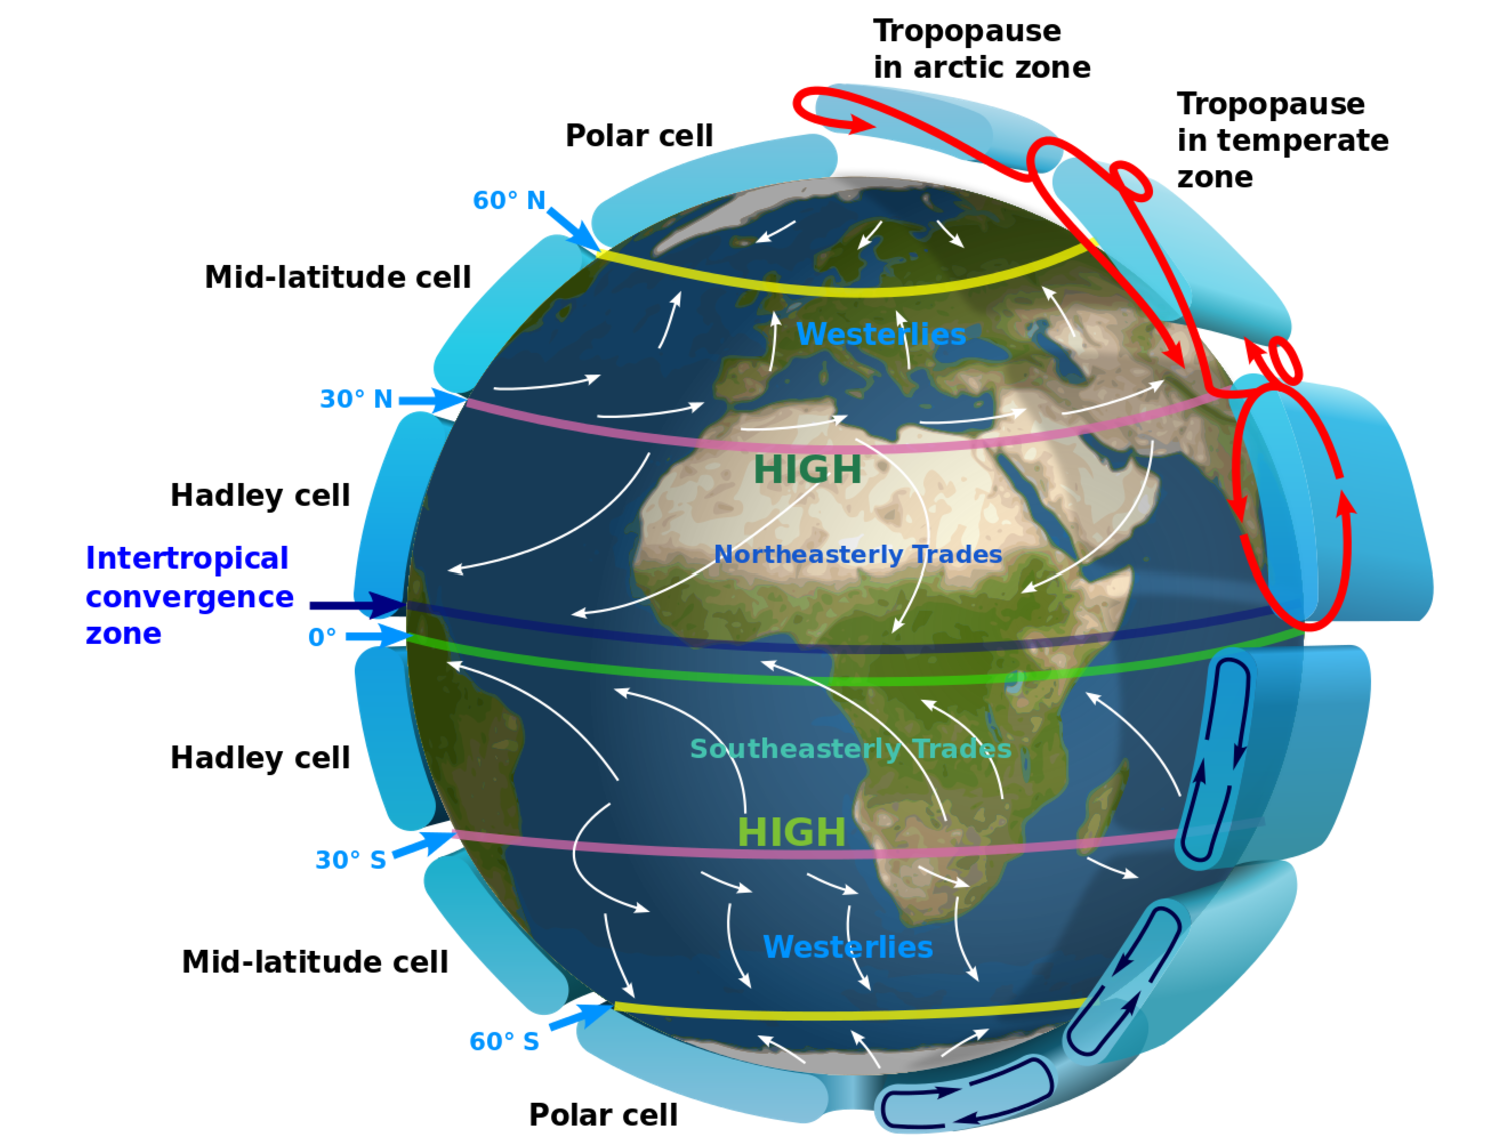
\includegraphics[width=0.5\linewidth]{upload/GAC.png}
	\caption{Global Atmospheric Circulation cells}
	\label{fig:GAC}
\end{figure}

In reality, the atmospheric circulation is more complex than the three-cell model suggests. It exhibits significant temporal and spatial variations due to factors like land/sea contrasts, topography, and changes in solar heating. While the model serves as a foundational framework, modern climate science relies on satellite data and simulations for a detailed understanding of global atmospheric dynamics.



\paragraph{Monsoons and Land Sea breezes:} they are wind patterns driven by differences in heating between land and water surfaces, but they operate on different scales.
\newline \textbf{Sea Breeze} (Daytime): During the day, land heats up faster than water, causing air over the land to rise and creating a low-pressure zone. Cooler, denser air from over the sea flows in to replace it, generating a breeze from sea to land.
\newline \textbf{Land Breeze}(Nighttime): At night, the land cools faster than water, creating a high-pressure zone over the land. Air flows from the land to the sea, forming a weaker land breeze.
\newline \textbf{Summer Monsoon}: Similar to a large-scale sea breeze, during summer, land masses (like South Asia) heat up more quickly than the surrounding oceans. This creates a low-pressure zone over land, drawing in moist air from the Indian or Pacific Oceans. The moisture-laden air rises and cools, resulting in heavy rainfall, particularly over mountain ranges like the Himalayas and Ghats.
\newline \textbf{Winter Monsoon}: In winter, the land cools faster than the ocean, forming a high-pressure zone. Cold, dry air flows outward from the land to the sea, leading to dry weather conditions over most of South Asia.
\newline Key Differences:while land/sea breezes are localized and operate on a daily cycle, monsoons occur over larger areas and are seasonal, driven by shifts in the Intertropical Convergence Zone (ITCZ).
Monsoons involve additional complexities, including the influence of upper atmospheric circulations, such as the jet stream.
The Asian monsoon, particularly over South Asia, is the most prominent example, crucial for regional agriculture and ecosystems. However, its dynamics are far more complex than those of simple land and sea breezes.

\subsection{The time averaged zonal general circulation}
The time-averaged circulation, computed from ERA5 Reanalysis data, shows westerly mid-atmosphere jets in the subtropical regions of both hemispheres. These jets reach a maximum around the 200mb level (\~12 km) and extend to the surface in the mid-latitudes, while easterly flows dominate the equatorial zone. The jets exhibit a strong seasonal cycle, with accelerated jets in winter and weaker jets in summer. There is a seasonal poleward migration of the jet cores, with the winter season showing more concentrated and intense maximums. The Southern Hemisphere's winter jet is broader than its Northern Hemisphere counterpart, both linked to the stratospheric flow above.

The stratosphere also exhibits strong jets with a stronger seasonal cycle, where easterlies replace westerlies as the seasons change. In the meridional circulation, low-level convergence occurs at the equator, with high-level divergence. The InterTropical Convergence Zone (ITCZ) oscillates between 15°N and 5°S, influenced by the seasonal cycle of the sun.

Temperature decreases with latitude due to radiation balance, with the equator receiving more solar radiation than the poles. The temperature decreases with height in the atmosphere, though the lapse rate is less than adiabatic, indicating a generally stable atmosphere. There is a strong latitudinal temperature gradient, which weakens with altitude and reverses in the upper atmosphere and stratosphere, due to radiation absorption by ozone and other components in the lower stratosphere.

The reversal of the meridional temperature gradient aligns with the zonal wind structure, showing positive shear in the troposphere and negative shear above, consistent with thermal wind balance. Water vapor, measured as specific humidity, is concentrated in the lower atmosphere and the equatorial region, with significant dryness at higher altitudes. The atmosphere's moisture content decreases with altitude due to the Clausius-Clapeyron relation, which links water vapor pressure to temperature. At the equator, moist air contains 12-15 grams of water per kilogram of air.

Specific humidity follows the seasonal cycle of the sun, shifting latitudinally. The maximum is located around 5°S in December-February (DJF) and around 10°N in June-July-August (JJA). The winter hemisphere is more moist at the surface than the summer, though values in the winter are smaller than in the equatorial zone, reaching up to 8 g/kg.

\subsection{The horizontal general circulation and wind }

The climatological geopotential height at 200mb shows deviations from a zonally symmetric circulation, particularly over the east coasts of continents, downstream from major mountain ranges like the Rockies and Himalayas. These features are clearer with specialized projections, highlighting the winter atmospheric pattern. While geopotential height can approximate wind flow in mid-latitudes, wind analysis is more useful in low latitudes.

At 200mb, winter jet streams are strong in both hemispheres, especially over Asia, with the Asian jet reaching velocities over 70 m/s. The Southern Hemisphere jet is weaker. In summer, westerly jets are weaker, and easterly jets dominate the tropics. The Indian Ocean sees a strong easterly flow in summer, leading to divergence over South America and Indonesia.

The meridional wind shows alternating poleward and equatorward patterns in winter, with large deviations in the Pacific-North American sector and East Asia. In summer, winds weaken but remain stronger in the Southern Hemisphere. Near the surface, the zonal wind is stronger over oceans and weaker over land, with easterlies in the subtropics, except in the Indonesian region, where westerlies prevail. The equatorial Pacific shows a convergence zone.

During JJA, the seasonal cycle strengthens winter wind features, with strong westerlies in the Indian Ocean signaling the start of the South Asian Monsoon. The meridional wind shows an equatorward flow along continent coasts, intensifying in summer, and reversing along the Somali coast.

At the 850mb level, trade winds dominate the equatorial Pacific, shifting with the ITCZ’s seasonal cycle. The Asian Summer Monsoon is visible in the Indian Ocean, forming a large gyre from East Africa to the Indian subcontinent, crucial for understanding low-level atmospheric and oceanic interactions.

\subsection{Mean Sea Level Pressure and The Sea Surface Temperature}
(MSLP) is a key parameter in describing atmospheric circulation. It represents the atmospheric pressure adjusted to mean sea level, though its usefulness is limited in areas with significant mountains, like the Rockies, Himalayas, and Antarctica, where the concept of "sea level" is effectively underground. Outside these areas, MSLP provides a good representation of atmospheric mass distribution. High MSLP areas correspond to mass accumulation, particularly in the subtropics, where high-pressure systems are common in both summer and winter.

Near-surface temperatures, typically measured 2 meters above the ground, reflect the seasonal and geographical variation in temperature. Over oceans, they follow sea surface temperature (SST), but land areas show significant seasonal changes. Northern continents are colder than the oceans at the same latitude, and coastal regions also experience temperature differences, with west coasts being milder than east coasts. In winter, high pressure tends to remain over land while low pressure develops over the oceans, reversing in summer. The intertropical zone sees high-pressure centers shifting with the seasons, while the Southern Hemisphere features a more symmetric pattern, with a ring of low pressure around Antarctica.

The seasonal cycle is evident in the shift of high-pressure areas in the tropics, moving latitudinally with the changing seasons. The meridional distribution of sea level pressure shows high pressure in the tropics, with low pressure areas near the equator and in the mid-latitudes. In the Southern Hemisphere, the pressure gradients are stronger and more pronounced, with tropical pressure maxima shifting seasonally.

Sea Surface Temperature (SST) shows strong north-south gradients, with polar regions being cold and the equator generally warm. However, notable deviations from zonal symmetry occur near continental east coasts, particularly in the equatorial Pacific, where cold water intrudes at the equator in the East Pacific, contrasting with the warm waters of the West Pacific. These temperature differences highlight significant gradients in SST along the equator



\subsection*{The Role of Energy Processes}

The vertical temperature gradient in the atmosphere is maintained by complex energy processes, including the absorption and radiation of heat, convection, and interactions with the Earth's surface. These processes vary with latitude and season, creating the dynamic and layered structure of the atmosphere.

Inversions, which occur when surface air cools significantly, disrupt the usual temperature gradient, particularly in the troposphere. These events highlight the intricate balance of energy transfer within the atmosphere and its impact on weather and climate.

\subsubsection{Energy balances }
To understand how the atmosphere maintains the various temperature structures, it is necessary to consider the processes by which the atmosphere gains and loses energy and how these processes vary with latitude and season. Essentially all the energy that enters in the climate system comes from the sun, part of it is absorbed in the system and must be balanced with outgoing energy leaving the system, to maintain the overall climate system in its observed equilibrium state.

Because of the different temperatures between the sun and the Earth, the energy emitted by the two bodies is sharply different. The spatial and temporal distribution of the receipt of solar energy at the Earth’s surface is highly dependent upon the Earth's annual revolution around the sun, its daily rotation about its axis, and the tilt of its axis concerning the plane of its orbit.

When the Earth is in the portion of its orbit where the Northern Hemisphere is tilted toward the sun, the Northern Hemisphere receives the majority of the direct sunlight and experiences summer, while the Southern Hemisphere experiences winter. Naturally, the reverse occurs when the Earth is in the opposite portion of its orbit, with the Southern Hemisphere tilted toward the sun.

About half of the incoming solar radiation is absorbed by the Earth's surface. This energy is transferred to the atmosphere by warming the air in contact with the surface (sensible heat), by evaporation and by thermal radiation that is absorbed by clouds and by greenhouse gases. The atmosphere in turn radiates thermal radiation back to Earth as well as out to space. Since all the
incoming radiation equals to $342 \,\, \text{Wm}^{-2}$ and $107 \,\, \text{Wm}^{-2}$ of it is reflected back to space, there must be
$235\,\, \text{Wm}^{-2}$ of terrestrial radiation emitted to space for an equilibrium situation from three main sources: water vapor, $CO_2$, clouds and Earth’s surface.

At the top of the atmosphere, the energy balance is composed of the compensating fluxes between the incoming solar radiation and the outgoing thermal radiation from the Earth. The solar radiation will be modulated by the reflectivity caused by the atmospheric cloud and in smaller part by the molecular components of the atmosphere itself. The thermal radiation will be modulated by the absorption properties of the atmosphere and its constituents. Both will be affected by the circulation and ultimately by the atmospheric flows.

The net balance shows a surplus of radiative flux in the subtropical region and a deficit in the polar regions. The global radiation budget can be obtained by integrating over the surface of the Earth the radiative fluxes.

At the surface, the energy balance involves more processes. There is also here a net solar radiation flux, modulated by the albedo of the surface and of the atmosphere, and a net thermal flux, obtained as the balance between the radiation emitted by the surface and the downward flux coming from the bulk of the atmosphere. Then there is a sensible heat flux caused by the turbulent vertical motion that carries away heat through mechanical agitation and the latent heat flux that represents the heat necessary for the evaporation of water from the surface. Because of the extent of the ocean, the latent heat flux is an important element of the budget.

In addition, we can look at the total cloud cover which is essentially the aggregated quantity of clouds at various levels. This is the quantity that is intuitively linked to the observation of a “cloudy sky”. In general, clouds are present over a vast surface of the globe. Some areas show a persistent absence of cloudiness over the entire year, such as the Sahara desert, part of the Arabian peninsula, Australia, and South Africa. Other areas instead show a strong seasonal cycle, with different could cover in different seasons. It is interesting to note that the seasonal cycle takes different characteristics in different areas. In the mid-latitudes cloud cover is larger in the local hemispheric winter than in the summer.

Looking at the zonal profile of the clouds, it is evident that major concentrations are related to the equator and middle/high latitudes.



\section{Oceans}
Oceans, covering approximately 71\% of Earth's surface, play a crucial role in global climate systems by storing and transferring heat, nutrients, and momentum. The interaction between the atmosphere and oceans significantly impacts weather and climate patterns. These bodies of water contain an estimated 1,350 million cubic kilometers of water, predominantly found in the Pacific, Atlantic, Arctic, and Southern Oceans, with an average depth of about 4,000 meters.
\newline Surrounding continents are continental shelves, shallow areas that extend outward for several kilometers before dropping sharply at the continental slope into the deep ocean floor. The ocean floor itself is varied, featuring features like underwater mountains, ridges, trenches, and smooth sedimentary basins.
\newline The oceans redistribute solar energy from equatorial to higher latitudes. As water warms at low latitudes, it absorbs significant amounts of solar heat. This heat is released into the atmosphere in the form of latent heat and longwave radiation as water cools or condenses, influencing global atmospheric circulation. Ocean currents further distribute this heat, balancing regional temperatures and aiding in climate regulation.(*)
\paragraph{Composition.} Seawater is not just water but a mixture containing various dissolved salts, with an average salinity of 35 grams per kilogram of water. This salinity largely comes from chloride, sodium, and sulfate, accounting for the majority of dissolved material. Salinity levels, however, vary globally. The Arctic Ocean shows lower salinity (~29\%), influenced by melting ice and freshwater inflows, while the subtropical Atlantic has some of the highest salinities (~37.5\%), due to high evaporation and low precipitation. These variations affect density, which in turn drives ocean circulation and temperature dynamics.
Overall, oceans are not only a storage medium for heat and nutrients but also critical in redistributing energy across the planet, moderating climate, and supporting ecosystems. Their interaction with atmospheric processes underscores their integral role in Earth's environmental systems.
\paragraph{Temperatures profiles.}
\subparagraph{Surface Temperatures:}
Range: -1°C (polar regions) to 20–30°C (tropics).
Seasonality: temperatures align in east-west zonal patterns, with exceptions like:
\begin{itemize}
	\item Tropical Pacific: western regions warmer than eastern regions due to currents.
	\item Gulf Stream: transports warm water northeast, moderating European climates.
\end{itemize}

\subparagraph{Temperature with Depth:}
\begin{itemize}
	\item Mixed Layer ($0–30$ m in summer):
	      warmed by sunlight and mixed by winds.
	\item Thermocline ($200–1000$ m):
	      sharp temperature gradient separating surface water from deeper layers.
	\item Deep Ocean ($>1000$ m):
	      uniform cold temperatures ($0.5–1.25°$C).
	\item Coldest water ($-0.25°$C) near Antarctica due to sinking dense, salty water from surface cooling and sea ice formation.
\end{itemize}

\begin{wrapfigure}{R}{0.5\textwidth}
	\begin{center}
		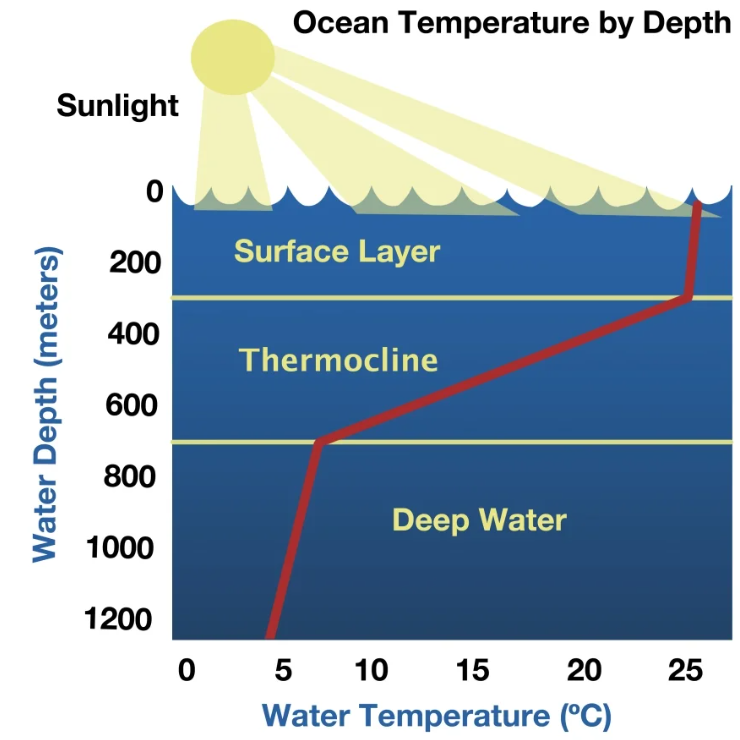
\includegraphics[width=0.3\textwidth]{upload/Ocean T.png}
	\end{center}
	\caption{Ocean temperature diagram (unprecised values on the $y$-axis)}
	\label{}
\end{wrapfigure}



Ocean circulation is driven by temperature and salinity differences, influencing density and pressure. Surface currents are wind-driven, forming large gyres such as those in the Pacific and Atlantic Oceans. These gyres redistribute heat and nutrients, shaping regional climates and ecosystems. Deep ocean currents, part of the thermohaline circulation\footnote{\url{https://rwu.pressbooks.pub/webboceanography/chapter/9-8-thermohaline-circulation/}}, involve the sinking of dense, cold water and the upwelling of warmer, nutrient-rich water, critical for sustaining marine life.
Additionally, mesoscale eddies, swirling water masses, play a significant role in transporting momentum, heat, and nutrients horizontally and vertically, although their dynamics are not fully understood. These processes together illustrate the complex and vital role oceans play in regulating Earth's climate and supporting life.
\begin{figure}[htbp]
	\centering
	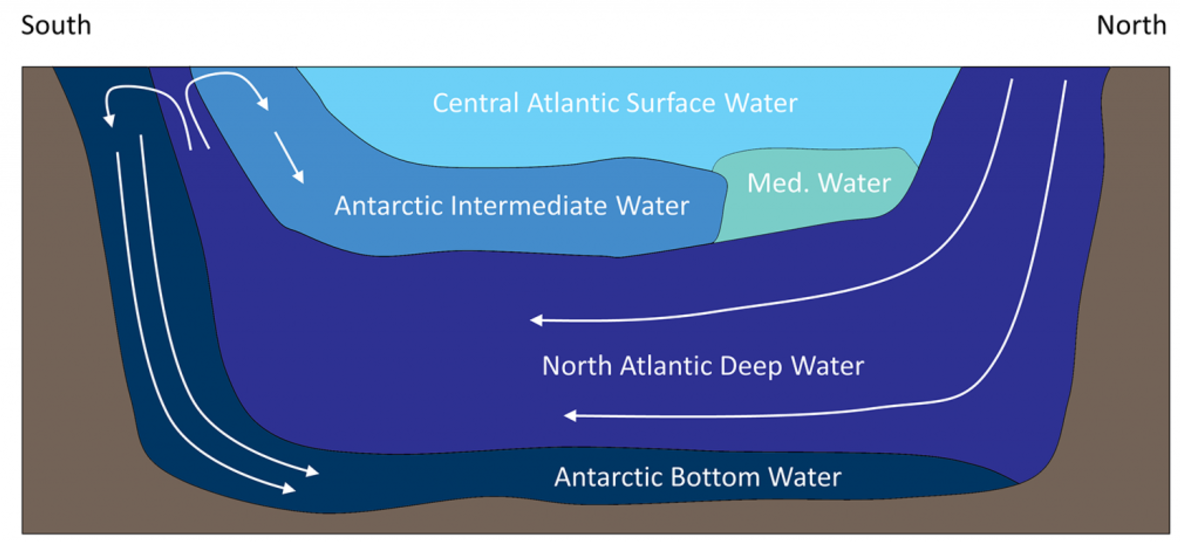
\includegraphics[width=0.5\linewidth]{upload/atlocean.png}
	\caption{The major water masses of the Atlantic Ocean}
	\label{fig:enter-label}
\end{figure}
\\
[0.1cm]

\subsection{The salinity structure of the ocean }
The salinity structure of the oceans is shown in Figure \ref{fig:fig1}.  The top panel shows the salinity near the surface at a nominal depth of
5m. We notice that there is a complex structure with low salinity
(fresher) waters at the poles and progressively more saline water moving towards the Equator, but then salinity decreases again at the equator. It is probably instructive to look at the latitudinal distribution of the precipitation. We can notice that the peaks of precipitation in the midlatitude and at the Equator are correlated with the low-salinity areas, whereas the subtropical regions are regions of strong evaporation, whose signature is the high salinity of the surface waters.

The Pacific Ocean is fresher than the Atlantic or even the Indian Ocean.
We can see from the map at 1000m that sources of saline waters are
marginal seas like the Mediterranean and the Persian Gulf. These areas
are evaporative basins that produce water so saline that it dominates
over the temperature effect and becomes denser so that we can find
Mediterranean water below the surface.
\begin{wrapfigure}{R}{0.5\textwidth}
	\begin{center}
		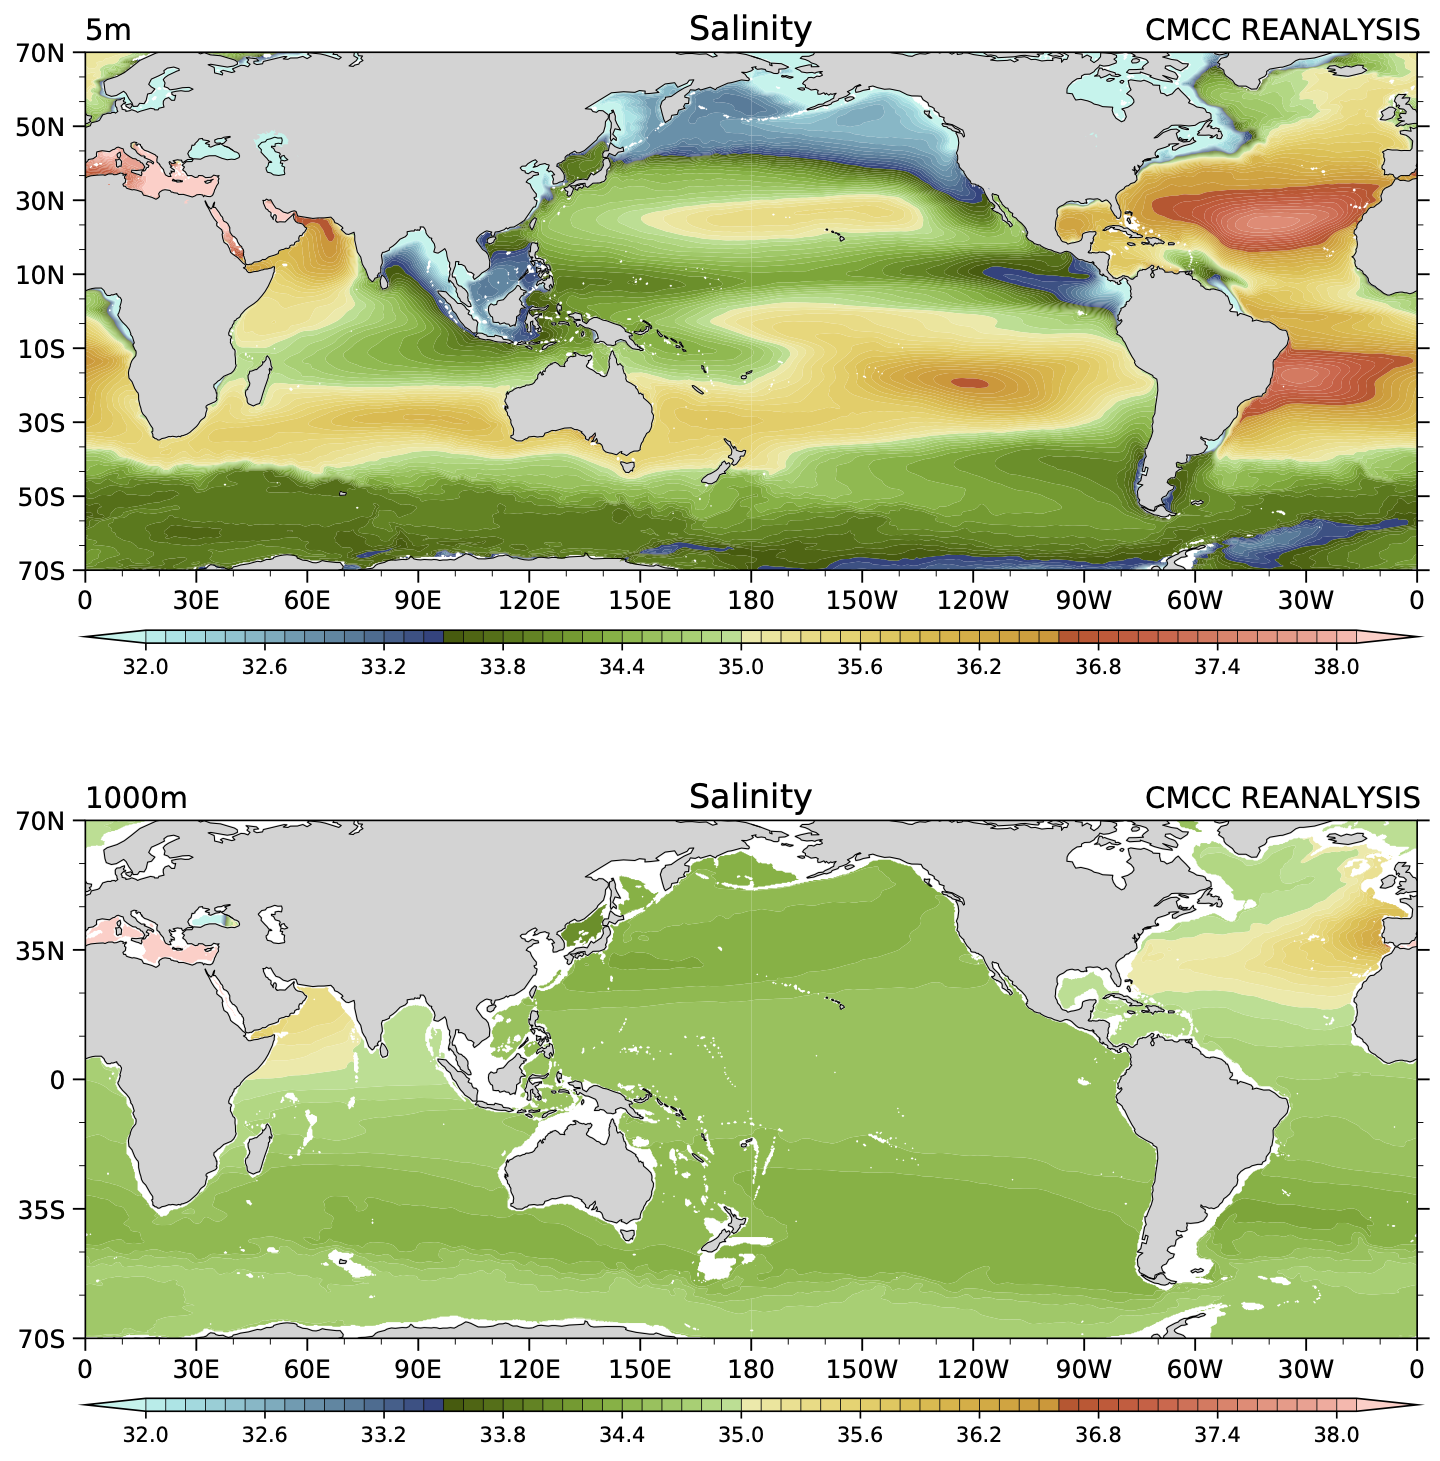
\includegraphics[width=0.48\textwidth]{upload/26image.png}
	\end{center}
	\caption{Salinity structure}
	\label{fig:fig1}
\end{wrapfigure}


The effect of the precipitation is less visible at the deeper depth pf
1000m (bottom panel), where the ocean tends to be fresher and more
uniform. We are using here the same scale to give a feeling of the
changes in salinity, except for the Atlantic and the east Indian Ocean,
the salinity is around 34 psu.
The effect of the runoff from major river systems is visible along the
Atlantic coast of South America where the Amazon river discharges and in the Bay of Bengal and around Indochina from the run-off the major rivers there, the Ganges and the Mekong.


In the pictures below: on the left salinity deviations with depth, going even deeper we have to change drastically
the scale. The oceans are remarkably uniform and the salinity deviations are really small. On the right, Pacific and Atlantic ocean salinity.



Looking at the North Atlantic (figures below) we notice that
there is a strong salinity gradient along the North American Coast that
follows roughly the pattern of the temperature gradient shown below. Strong temperature gradients are presumably to be
connected to the existence of currents, but we will need to check the
density, depending on the salinity later, to be sure.

\begin{minipage}{0.45\textwidth}\label{fig:fig4}
	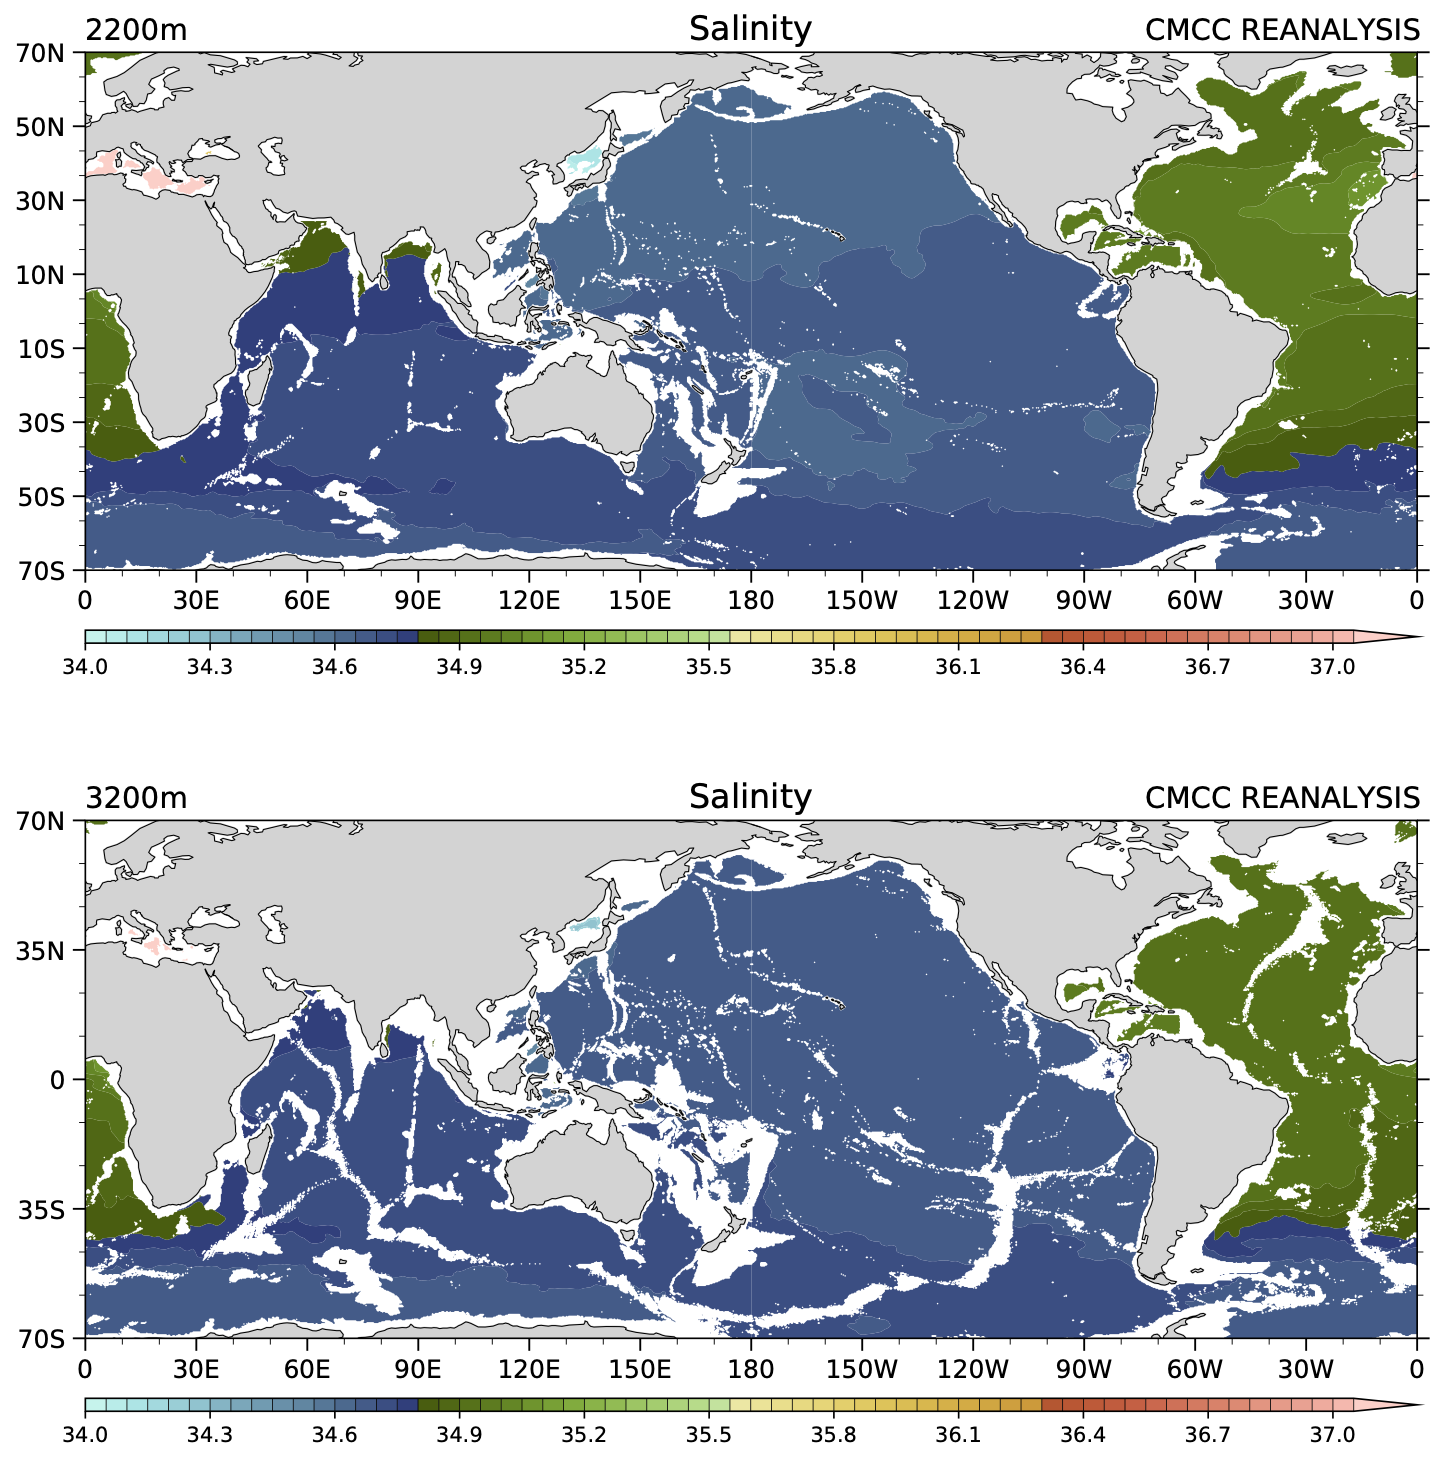
\includegraphics[width=0.9\textwidth]{upload/27image.png}
\end{minipage}
\begin{minipage}{0.45\textwidth}
	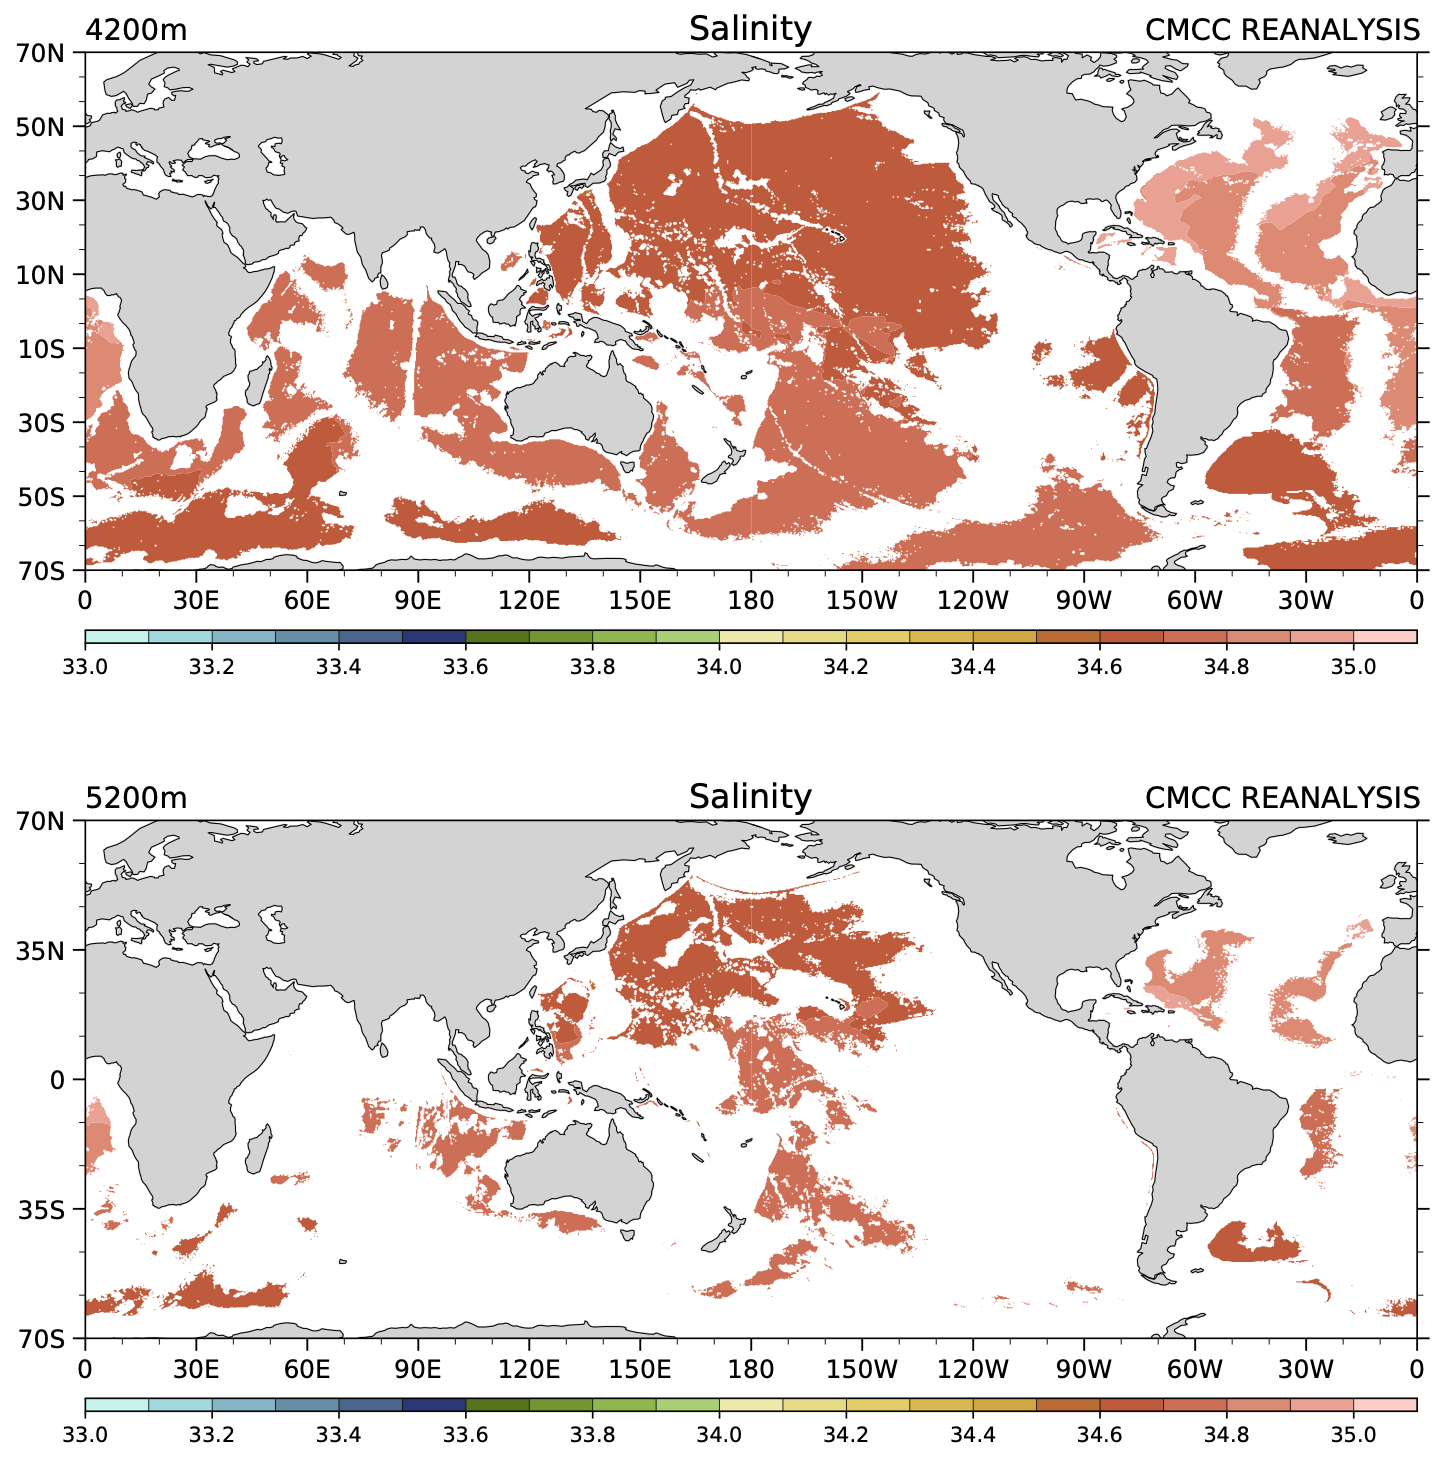
\includegraphics[width=0.9\textwidth]{upload/28image.png}
\end{minipage}\\
[0.1 cm]
Anyway,
this picture is giving a strong indication of the existence of something
remarkable and intense along the western boundary of the Atlantic ocean.


\begin{minipage}{0.45\textwidth}\label{fig:fig4}
	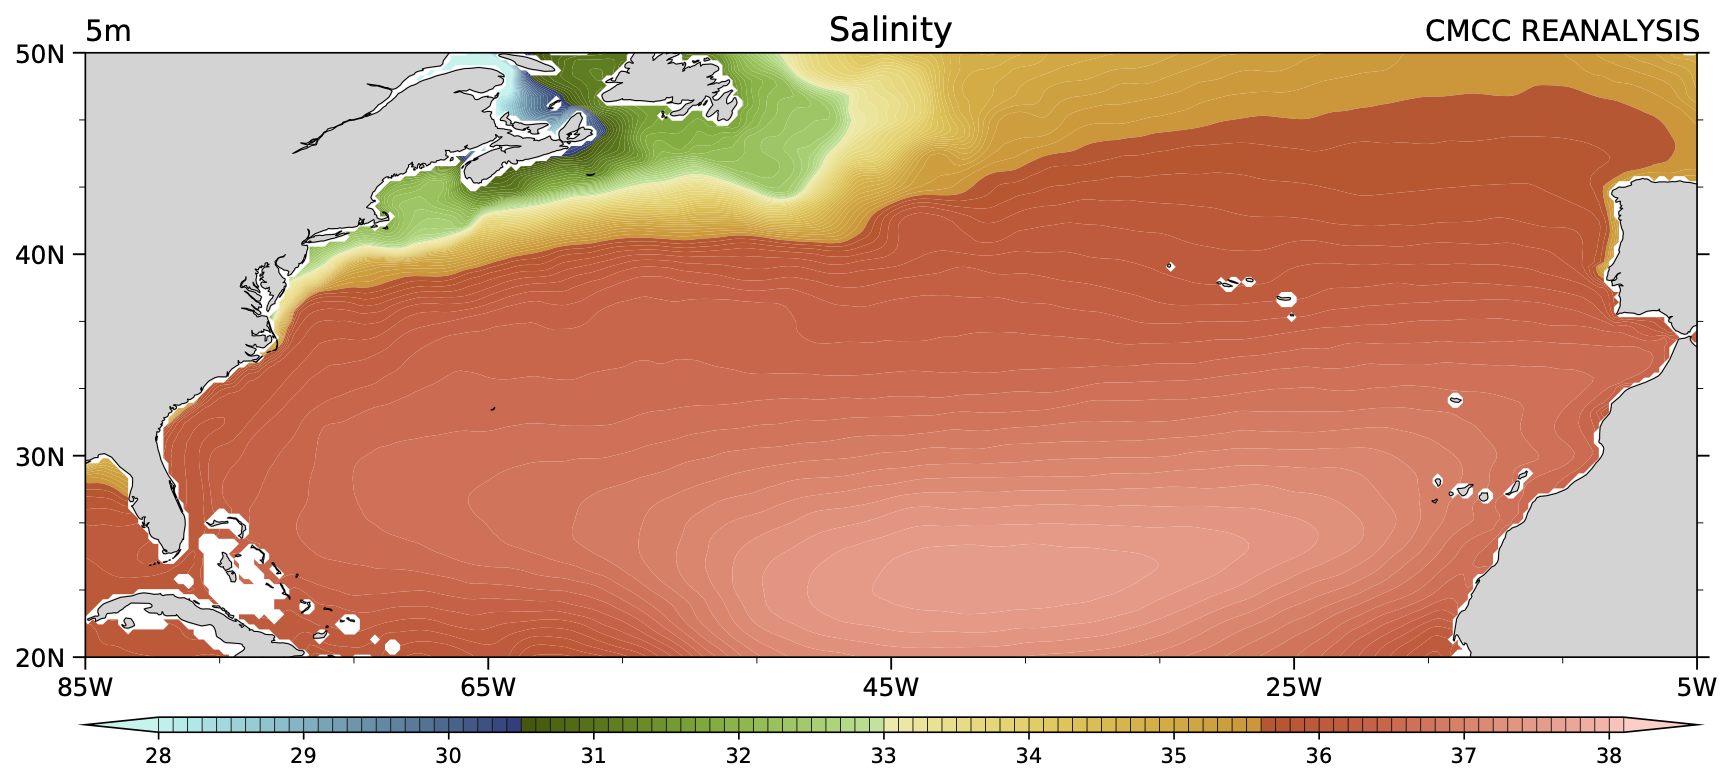
\includegraphics[width=0.9\textwidth]{upload/29image.png}
\end{minipage}
\begin{minipage}{0.4\textwidth}
	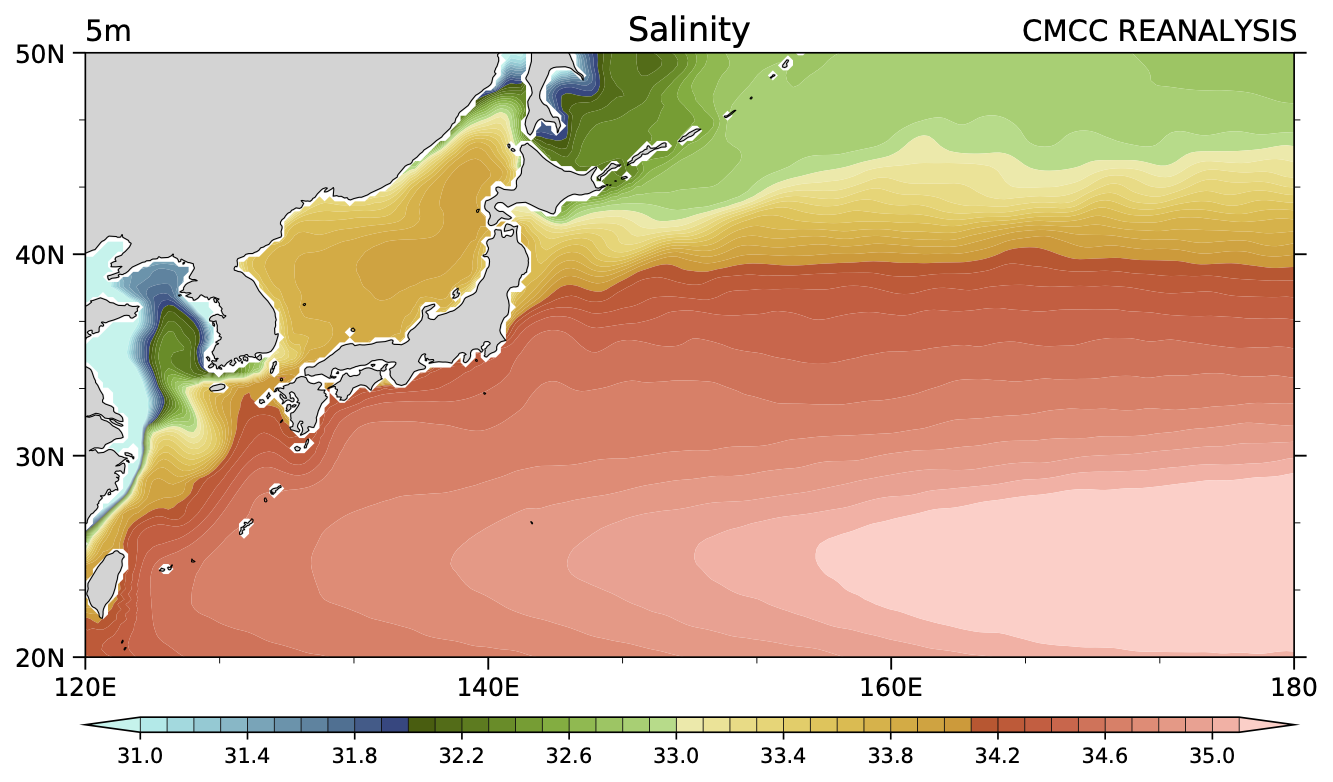
\includegraphics[width=0.9\textwidth]{upload/30image.png}
\end{minipage}\\


A similar situation exist in the North Pacific along the Japan coast and
therefore we can start to suspect that this has to do with the presence
of the continental boundary.

The previous analysis of the temperature is giving us hints of a strong
vertical structure of the oceans, so it may be useful to look at the
vertical distribution somewhat more in detail. The figures above show the same section North-South section of along the longitude of 25W, roughly in the middle of the Atlantic Ocean.
The salinity follows a similar pattern as the temperature with a
strong gradient approximately at the thermocline, the high salinity is
confined in thin; layers at the surface, but some interesting behaviour
is visible below. In the Northern Hemisphere we can see the
Mediterranean water penetrates at depth and actually protruding under the fresher water of Antarctic origin that is colder, but because is
fresher floats over the Mediterranean water. Really cold Antarctic water reaches the bottom, filling the abyssal plains of the basin.

\begin{figure}[htpb!]
	\centering
	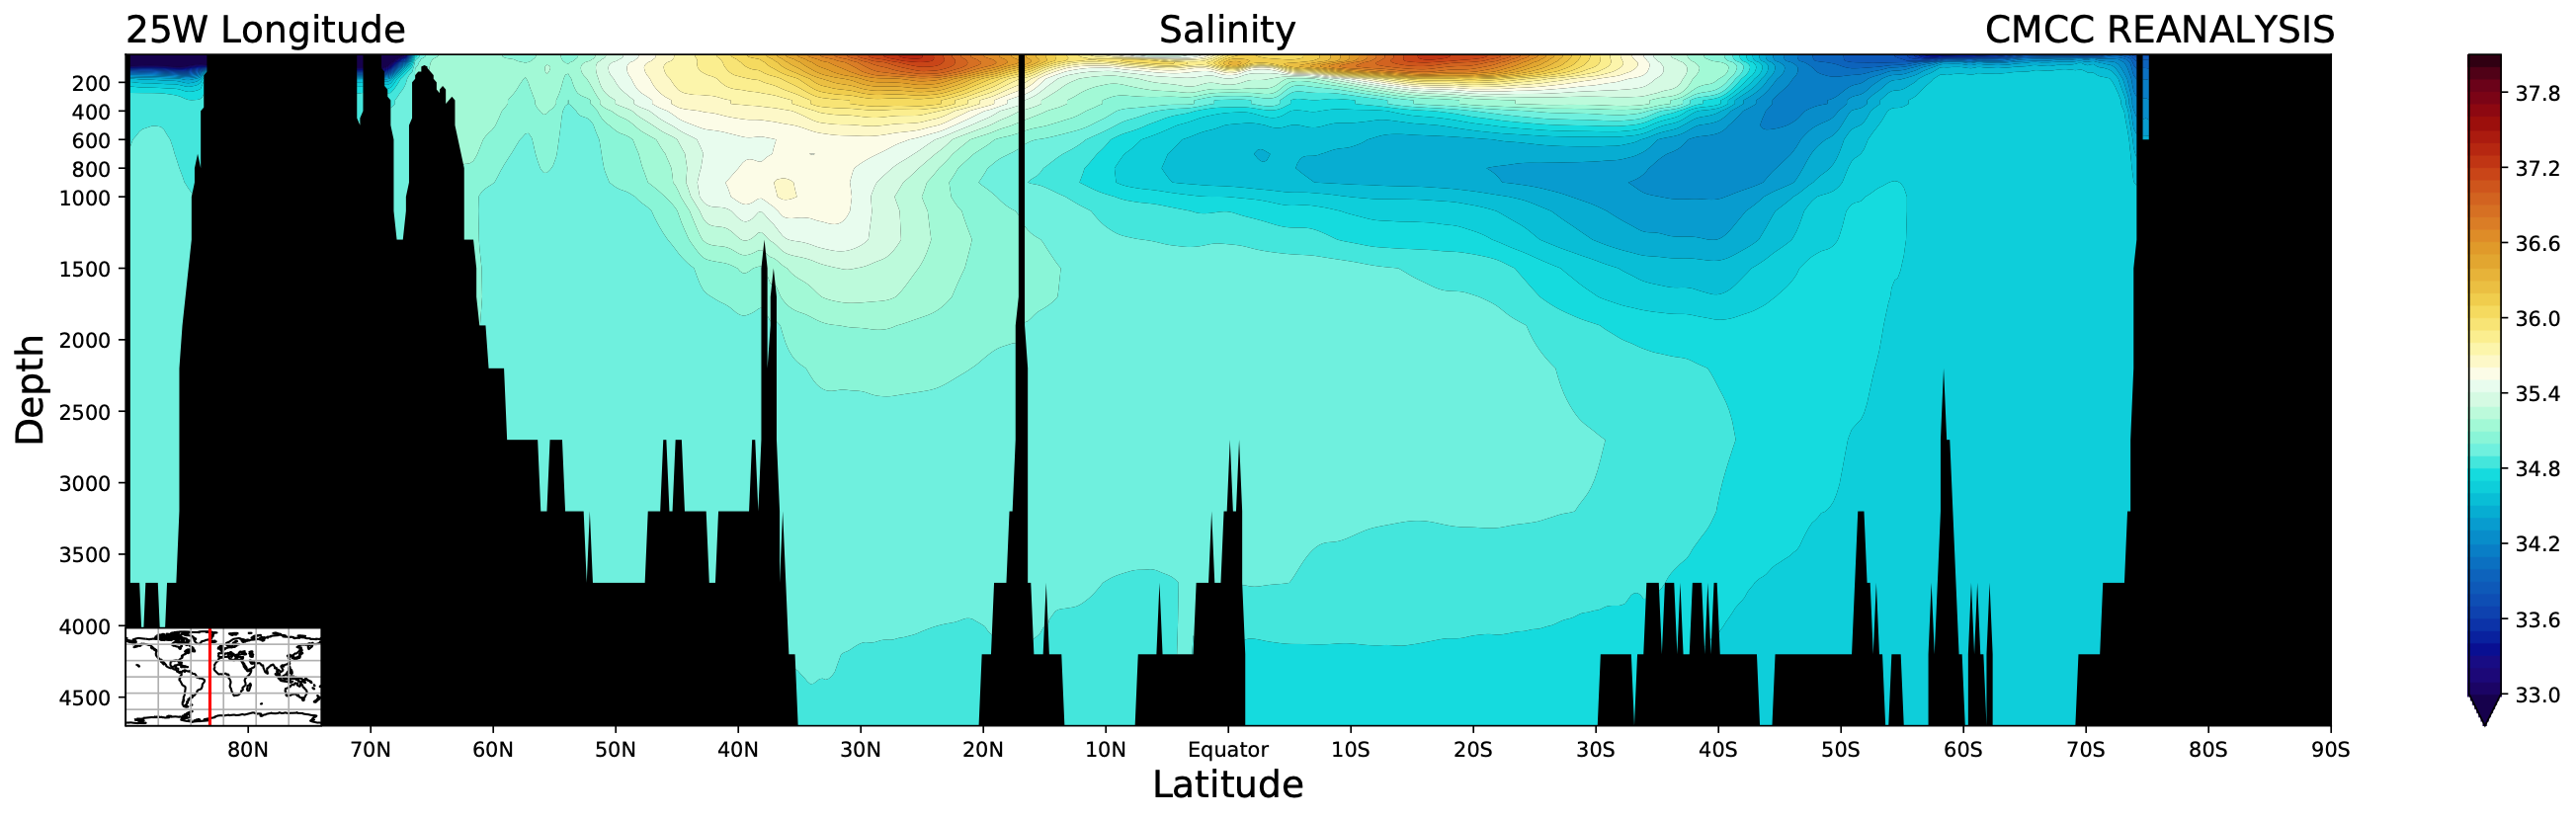
\includegraphics[width = 0.5 \textwidth]{upload/31image.png}
	\caption{North-South Salinity section at 25W longitude.}
	\label{fig:fig6}
\end{figure}

The Mediterranean waters are clearly visible in a longitude-depth
section (Figure \ref{fig:fig6}). The saline mediterranean water sinks
to about 1000m because it is warmer than the Atlantic but much more
saline so it is denser and it reaches an equilibrium depth at about
1000m.

\begin{figure}[htpb!]
	\centering
	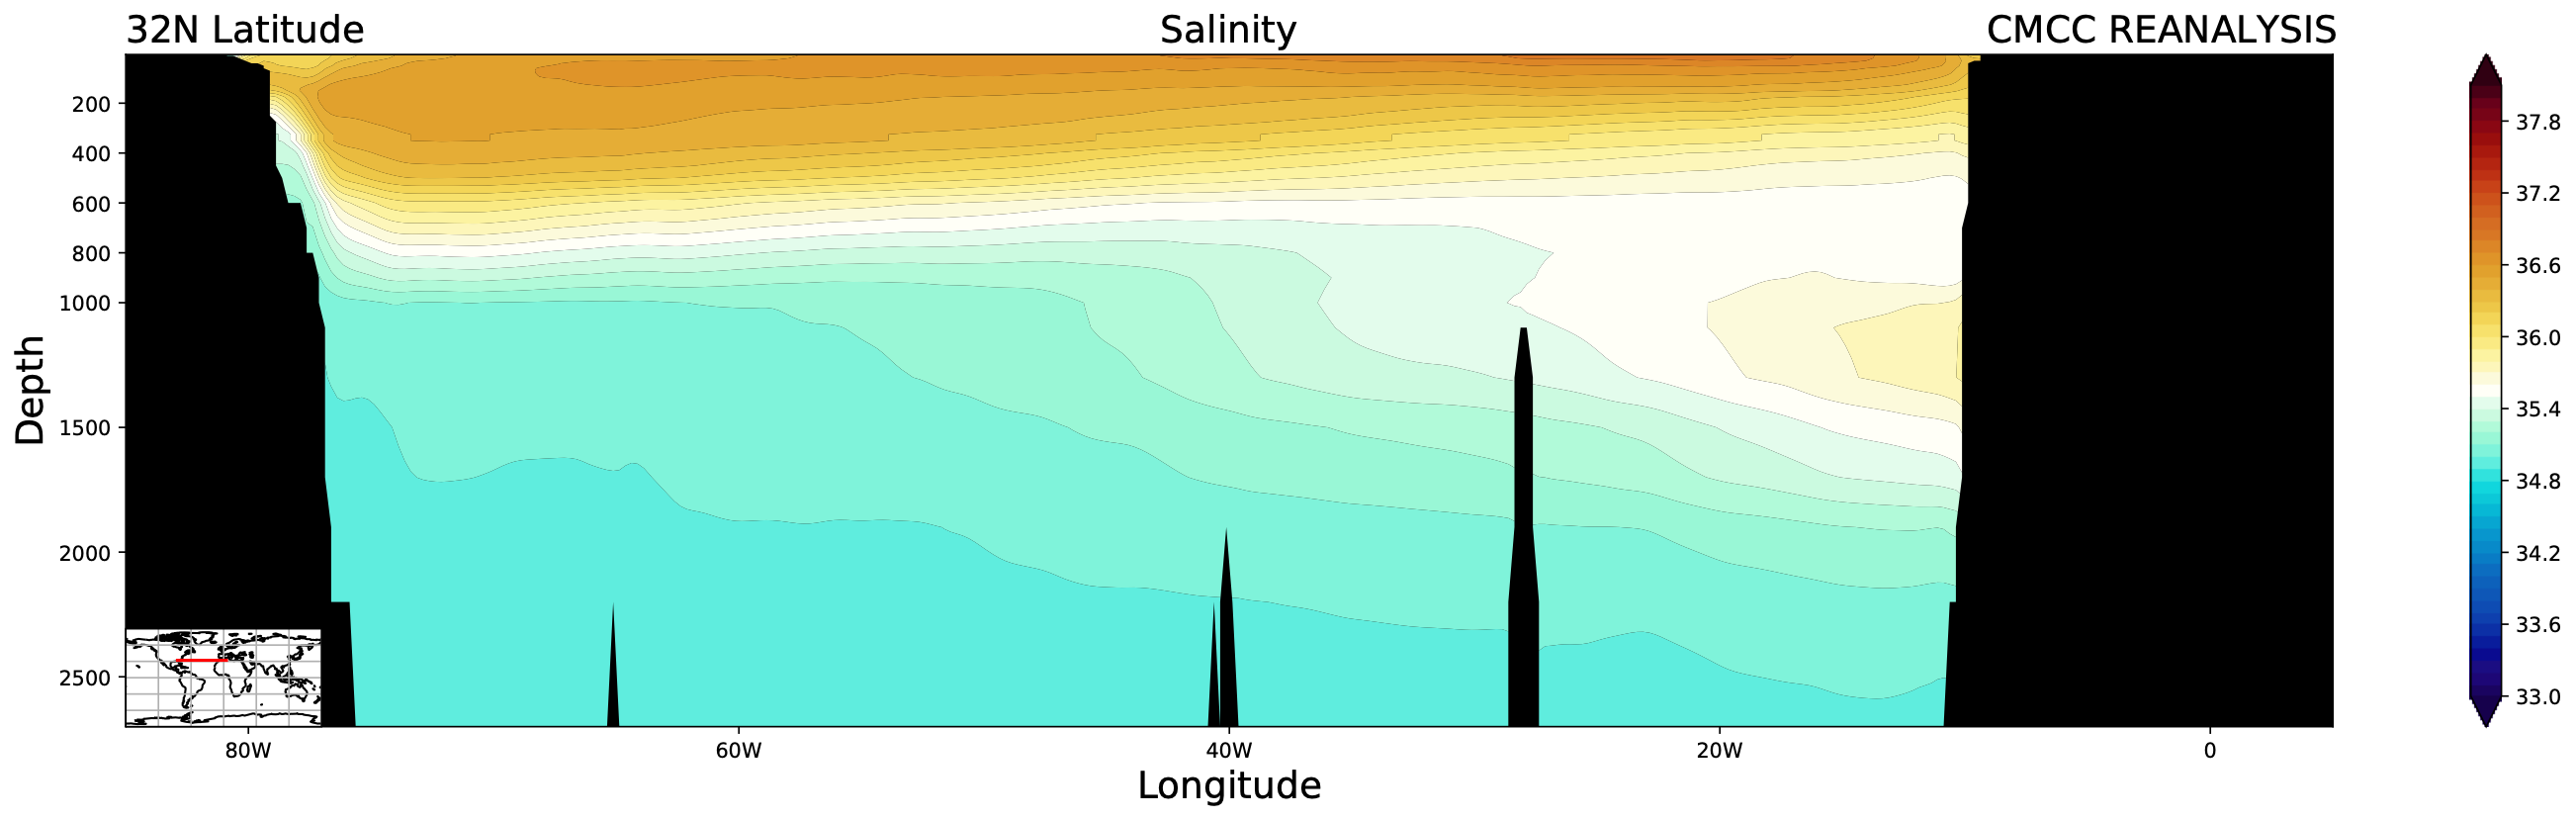
\includegraphics[width=0.5\linewidth]{upload/32image.png}
	\caption{The vertical structure of the Pacific Ocean}
	\label{fig:fig7}
\end{figure}


The vertical structure of the Pacific Ocean (Figure \ref{fig:fig7}) is
different and what we see is a situation where salinity is slowly
varying getting fresher toward the surface, with the thin saline water
in the subtropics a clear signature of the equatorial upwelling and the
Antarctic water filling the abyssal plains. The Indian Ocean is similar
to the Pacific South of the Equator but North of the Equator at this
longitude is fresher.

\begin{figure}[htpb!]
	\centering
	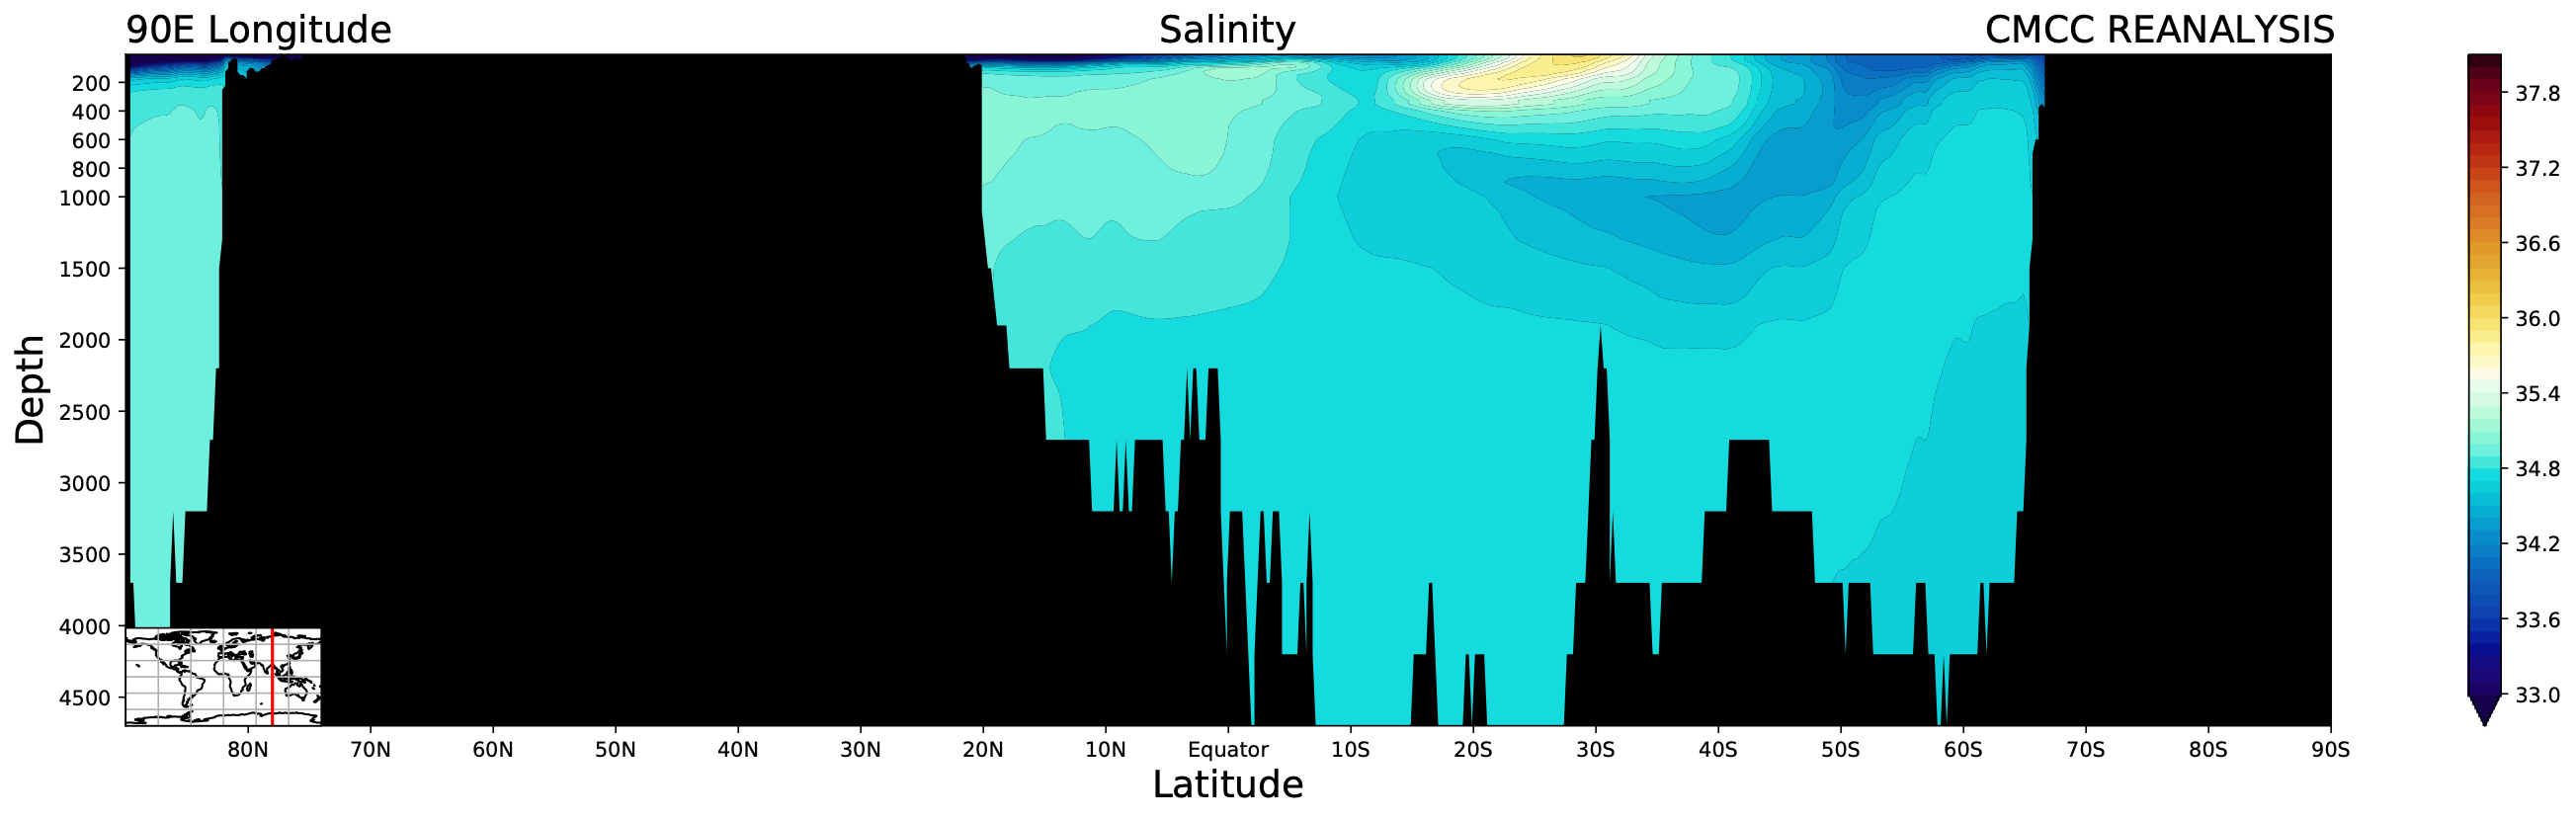
\includegraphics[width = 0.4 \textwidth]{upload/33image.png}
	\caption{As in Fig. \ref{fig:fig7} but for 90E longitude}
	\label{fig: fig8}
\end{figure}

The Indian Ocean (Figure \ref{fig: fig8}) shown here as a section
cutting essentially through the Bay of Bengal, shows a similar strong
stratification, but there are only weak signs of an equatorial upwelling
of cold water.



We can gain more insights in the equatorial structure by looking at a
longitudinal section along the Equator in the Pacific (Figure \ref{fig:fig9}). Here we see the general difference between the
Atlantic and the Pacific, but we also see that the salinity is following
the slant of the equatorial thermocline and the equatorial upwelling in
the East Pacific. The effect of the major precipitation center of ITCZ
in the West Pacific is visible in fresh water at the surface in the
West.

\subsection{Influence of the ocean}

\paragraph{The continentality effect}
It makes continental summers warmer and winters cooler than the adjacent ocean areas. The oceans have this effect because of their large heat storage capacity and because part of  the energy that they retain from solar input during the summer they return to the atmosphere in the forms of sensible and latent heat and longwave radiation the following winter. Conversely, the continents have the reverse effect, strengthening the seasonal temperature contrasts

\paragraph{Ocean currents}
They can transport heat from low to high latitudes. (in the Gulf Stream of the North Atlantic). This contributes to much higher winter air temperatures over mid-to-high latitude oceans than over adjacent land areas at the same latitude.

\paragraph{The overall basin
	circulation}\label{the-overall-basin-circulation}

The surface currents of the Atlantic ocean are shown in Figure \ref{fig:fig10}. As we might have suspected from the temperature coast that reaches all the way across the North Atlantic to Europe, the Gulf Stream. Strong currents are also visible in the Equatorial area
where they connect to the mid-latitude circulation forming a large circular system, the Subtropical Gyre. The South Atlantic has a similar gyre in the subtropical region, but at higher latitudes we can notice a strong westerly current cutting all along the basin, essentially along a latitude line between 40S and 50S.

\begin{figure}[htpb]
	\centering
	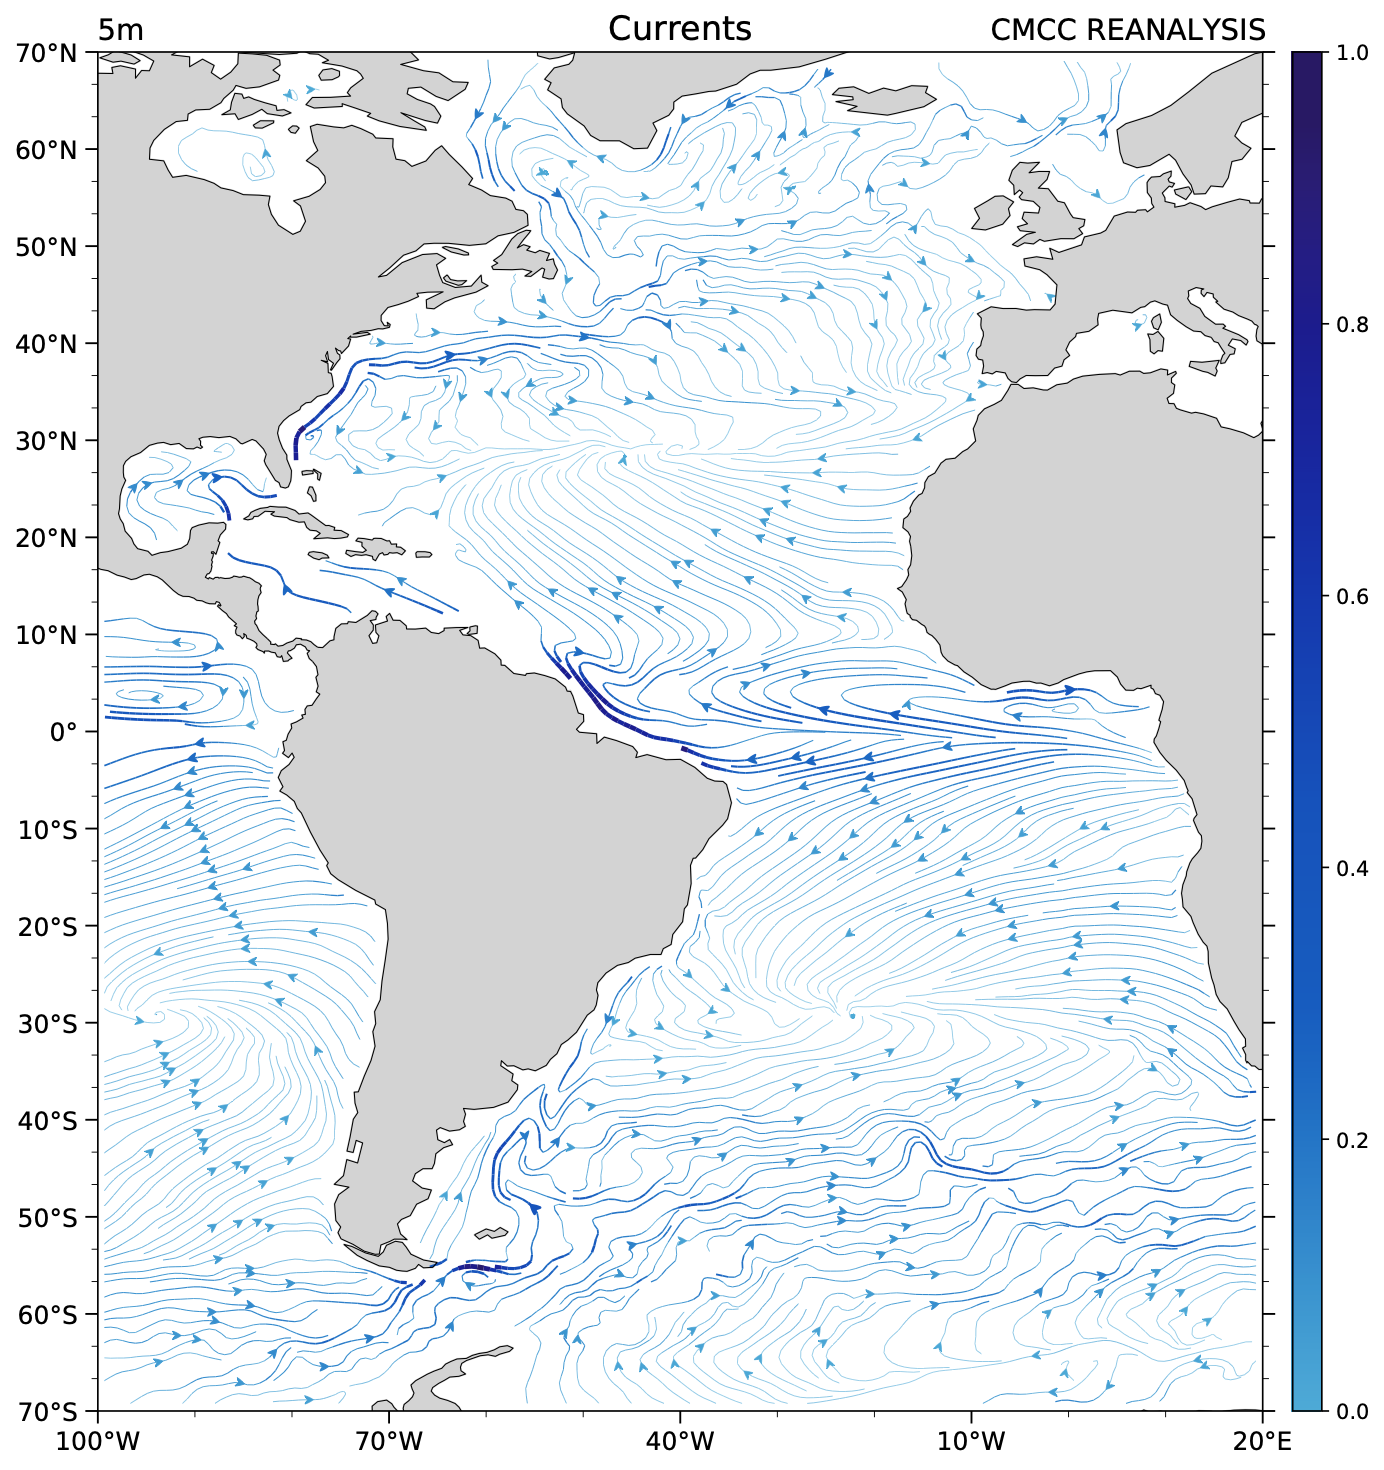
\includegraphics[width = 0.4 \textwidth]{upload/35image.png}
	\caption{The surface currents of the Atlantic ocean} \label{fig:fig10}
\end{figure}

The North Pacific surface circulation is shown in Figure \ref{fig:fig11}. We can notice here again a strong current along the Western boundary of the basin that than feed into a basin wide gyre that connects to the equatorial circulation. The boundary current, known her as the Kuroshio Current, is very narrow and intense along the Japan coast, as it is also the case of the Gulf Stream in the Atlantic, and it tapers into a wide system of streams and eddies into the open ocean.

It is possible to see also local system, like the small gyre off the Alaskan coast and similar circulation in the marginal seas, like the Sea of Okhotsk, near the Siberian coast. Their presence is remarkable as we are looking here at climatological averages over more than 40 years and so they are stable and persistent features. This is another reminder of how even relatively smaller feature in the ocean can be climatologically persistent over many years.

\begin{figure}[htpb]
	\centering
	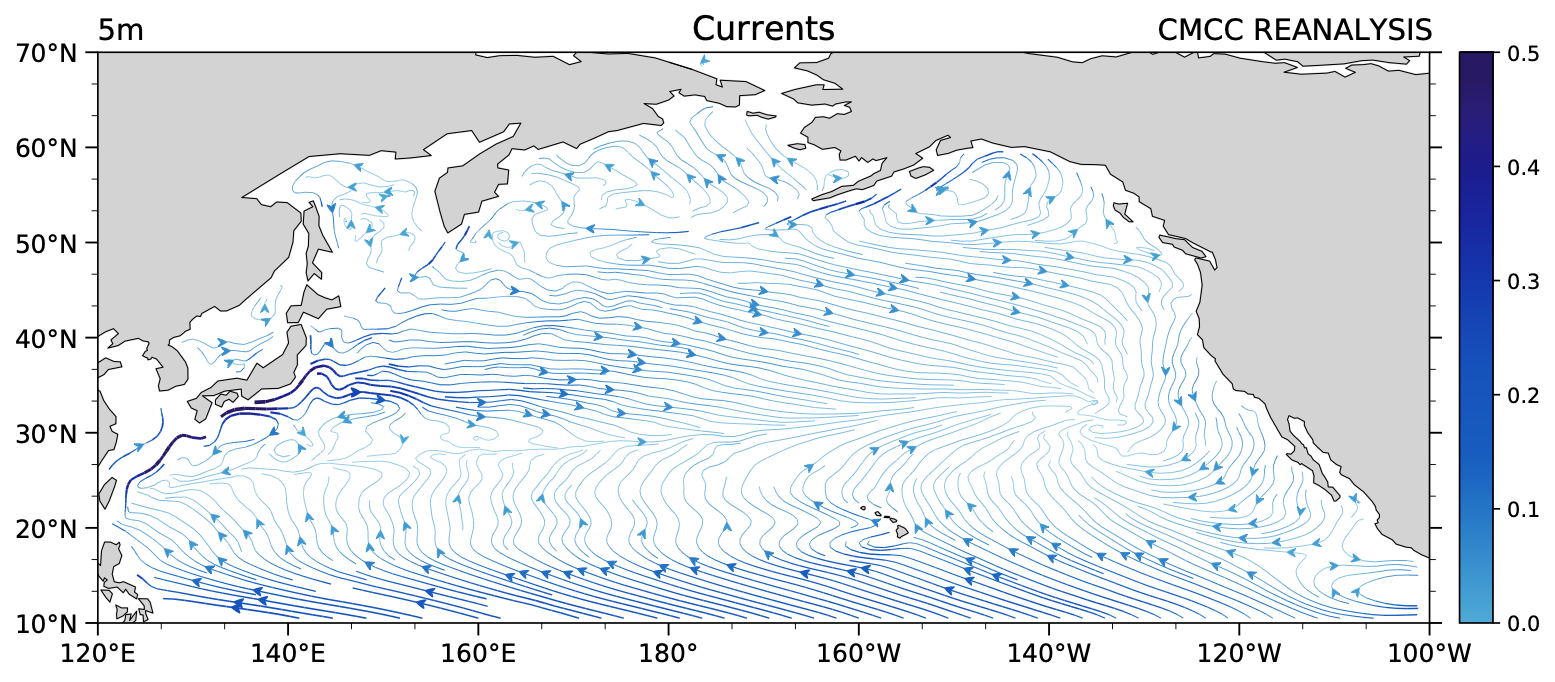
\includegraphics[width = 0.4 \textwidth]{upload/i36mage.png}
	\caption{The North Pacific surface circulation} \label{fig:fig11}
\end{figure}

The circulation of the South Pacific Ocean is shown in Figure \ref{fig:fig12}. The subtropical gyre is visible also here, but there is a weak indication of a western intensification current in the West pacific, close to the coasts of Australia and New Zealand. The strong high latitude current that we have seen in the Atlantic is also present here end evidently connect to the other basin through the Drake Passage, that is the Straits between South America and Antarctica.

\begin{figure}[htpb]
	\centering
	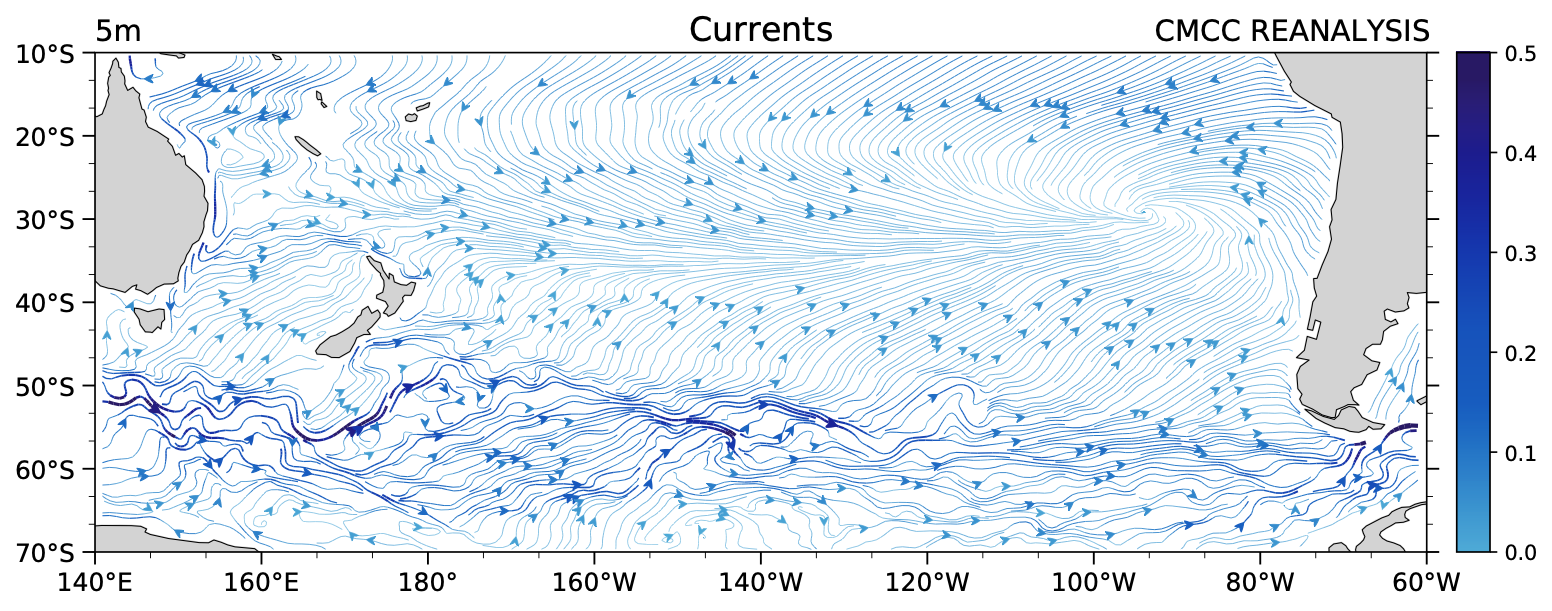
\includegraphics[width = 0.5 \textwidth]{upload/37image.png}
	\caption{The circulation of the South Pacific Ocean} \label{fig:fig12}
\end{figure}

The Indian Ocean circulation is shown in Figure \ref{fig:fig13}. The Indian Ocean is confined by continental masses in the north, so it is mostly composed of the equatorial region and the midlatitudes are all in the Southern Hemisphere. The subtropical gyre is present, together with features North of Madagascar. A boundary current develops on the African coast, The westerly current in the southern mid-latitudes is visible also here, strong and with a vigorous eddy field.

\begin{figure}[htpb]
	\centering
	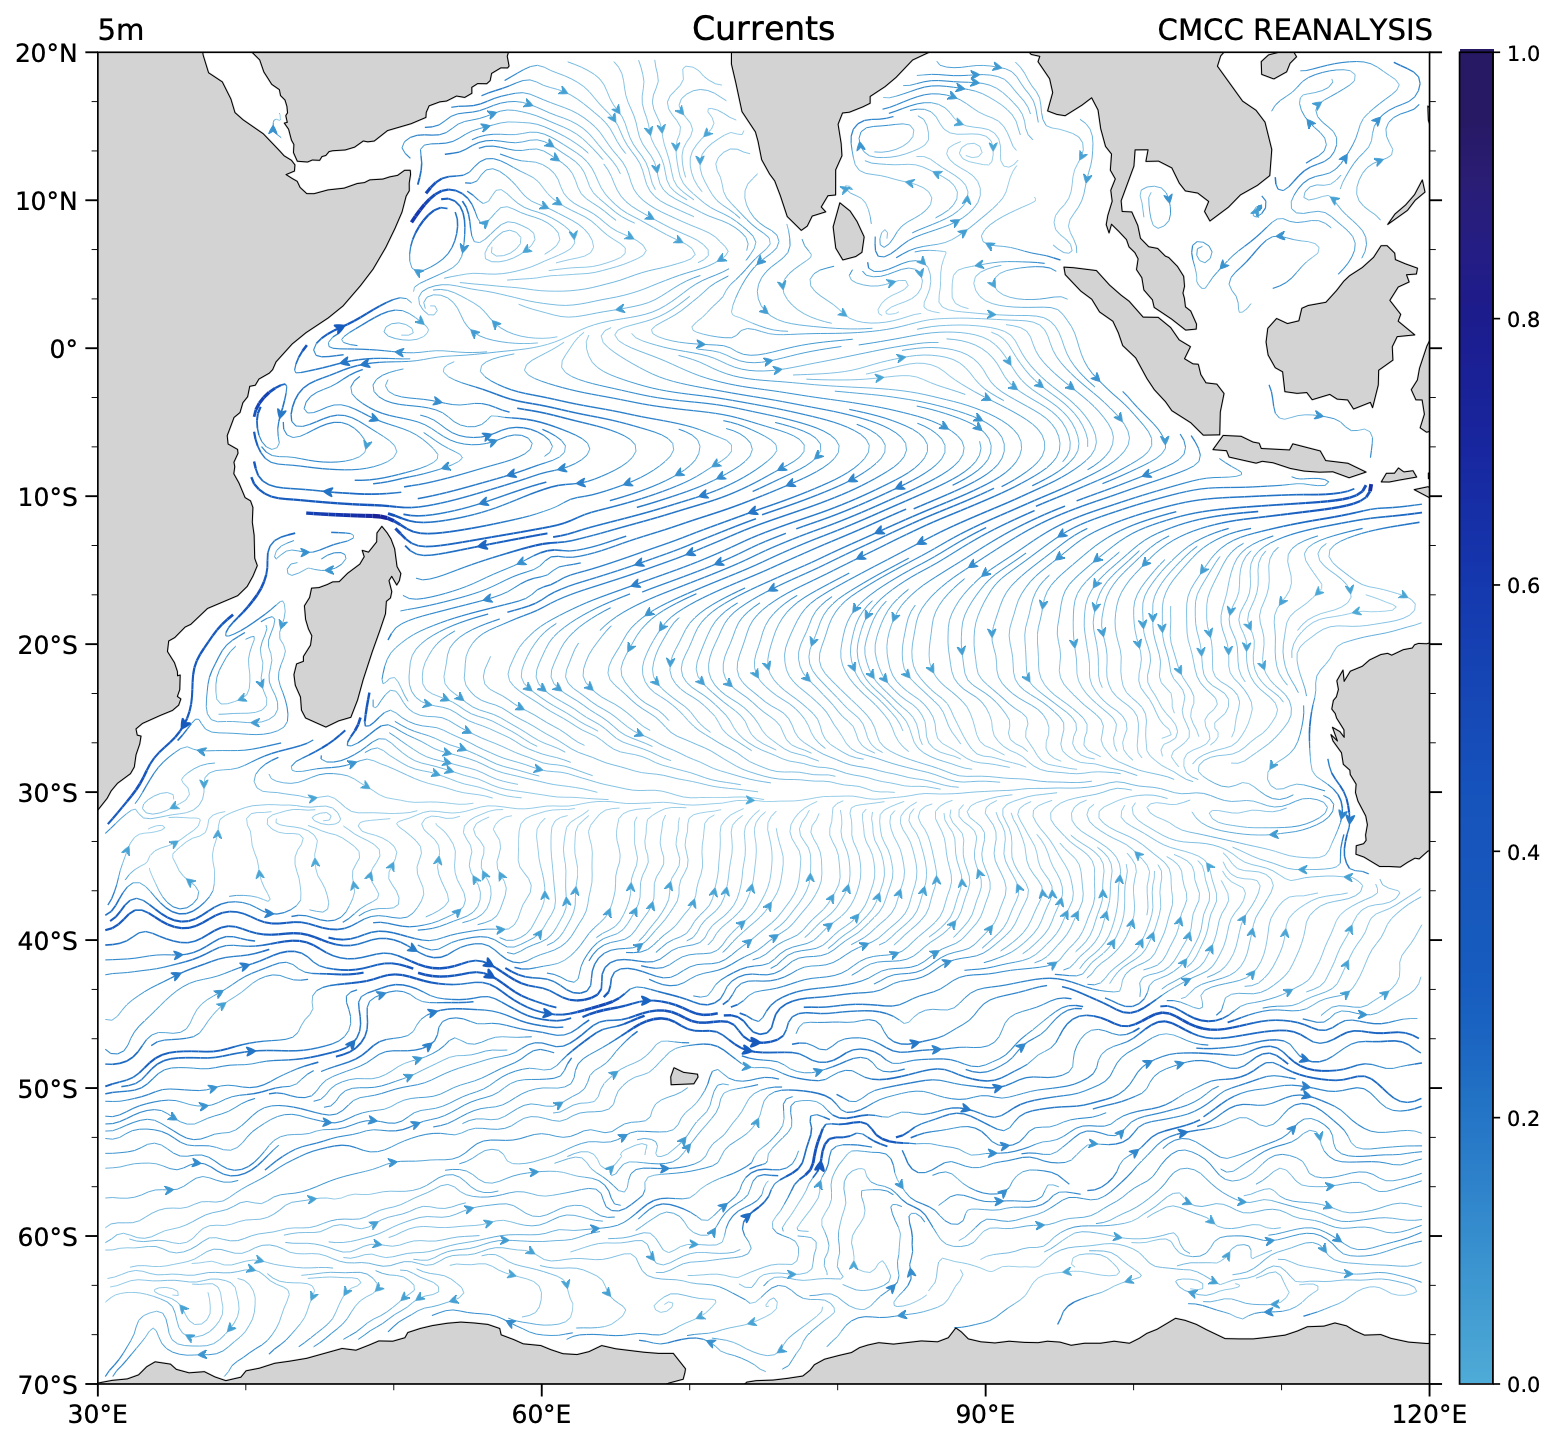
\includegraphics[width = 0.35\textwidth]{upload/38image.png}
	\caption{The Indian Ocean circulation} \label{fig:fig13}
\end{figure}

At this point we can suspect that there is probably a continuous ring of currents around Antarctica and this can be confirmed by the bottom panel of Figure \ref{fig:fig13}  that shows the entire extent around a
longitude circle of the current, known as the Antarctic Circumpolar
Current. It is a strong, highly turbulent system that connects all the
Ocean Basins.
\\

\subparagraph{The equatorial
	circulation}

The Equator is a special place for the atmosphere and so it is a special
place also for the Oceans. The circulation in this area is strongly
coupled with the atmospheric circulation and it is often characterized
by both westerly and easterly currents and by special behaviours right
at the Equator line. Futhermore, it is also very different from ocean to
ocean.

The equatorial current system in the Pacific Ocean is shown in Figure \ref{fig:fig14}. It is a complex system composed of two easterly
currents, the North and South Equatorial currents, sandwiching the
westerly Equatorial countercurrent. It is possible to notice that at the
Equator the currents are strongly easterly and diverging, leading to the
emergence of upwelling at the Equator by Ekman transport.

\begin{figure}[htpb]
	\centering
	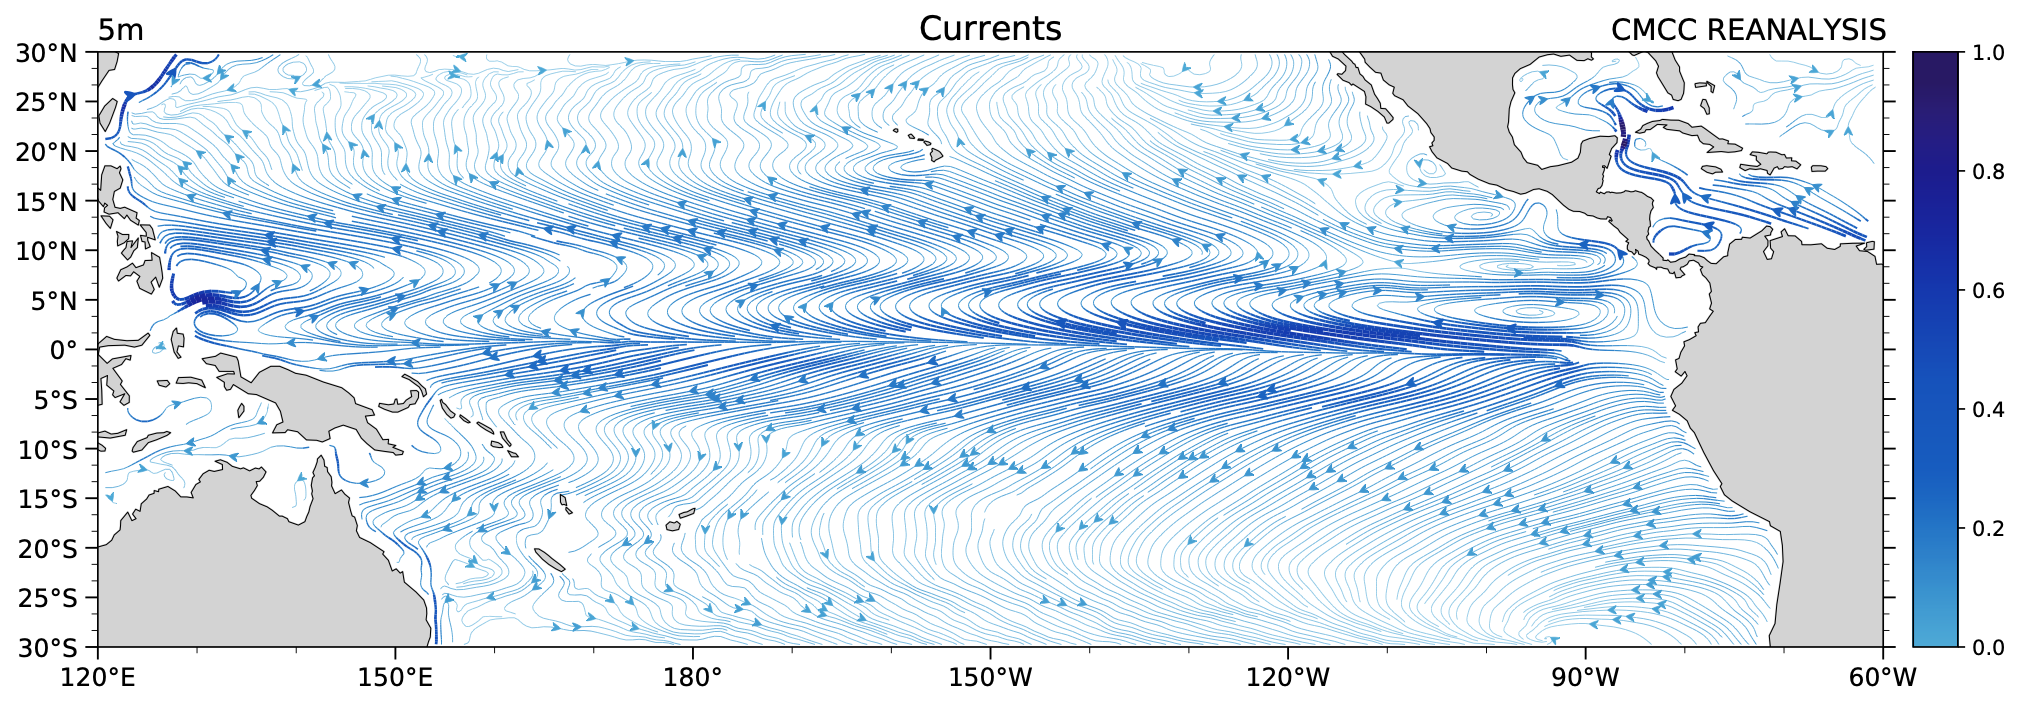
\includegraphics[width = 0.4 \textwidth]{upload/39image.png}
	\caption{The equatorial current system in the Pacific Ocean} \label{fig:fig14}
\end{figure}

The complexity of the equatorial current system can be further
appreciated by looking at the vertical section of the zonal current at
the Equator. A strong westerly current below the
surface, slanting from the West Pacific to the East Pacific, is visible
at depth between 200 and 300m. The speed is in excess of 1 m/s and it
gets progressively shallower in the East.

It is however part of an alternation of westerly and easterly currents
that become progressively weaker as they get deeper. They are centered
almost perfectly at the Equator, as it can be seen in Figure \ref{fig:fig16}. The latitudinal position of the undercurrent is very tightly controlled by rotational effects and it precisely tracks the position of the equatorial line.

\begin{figure}[htpb]
	\centering
	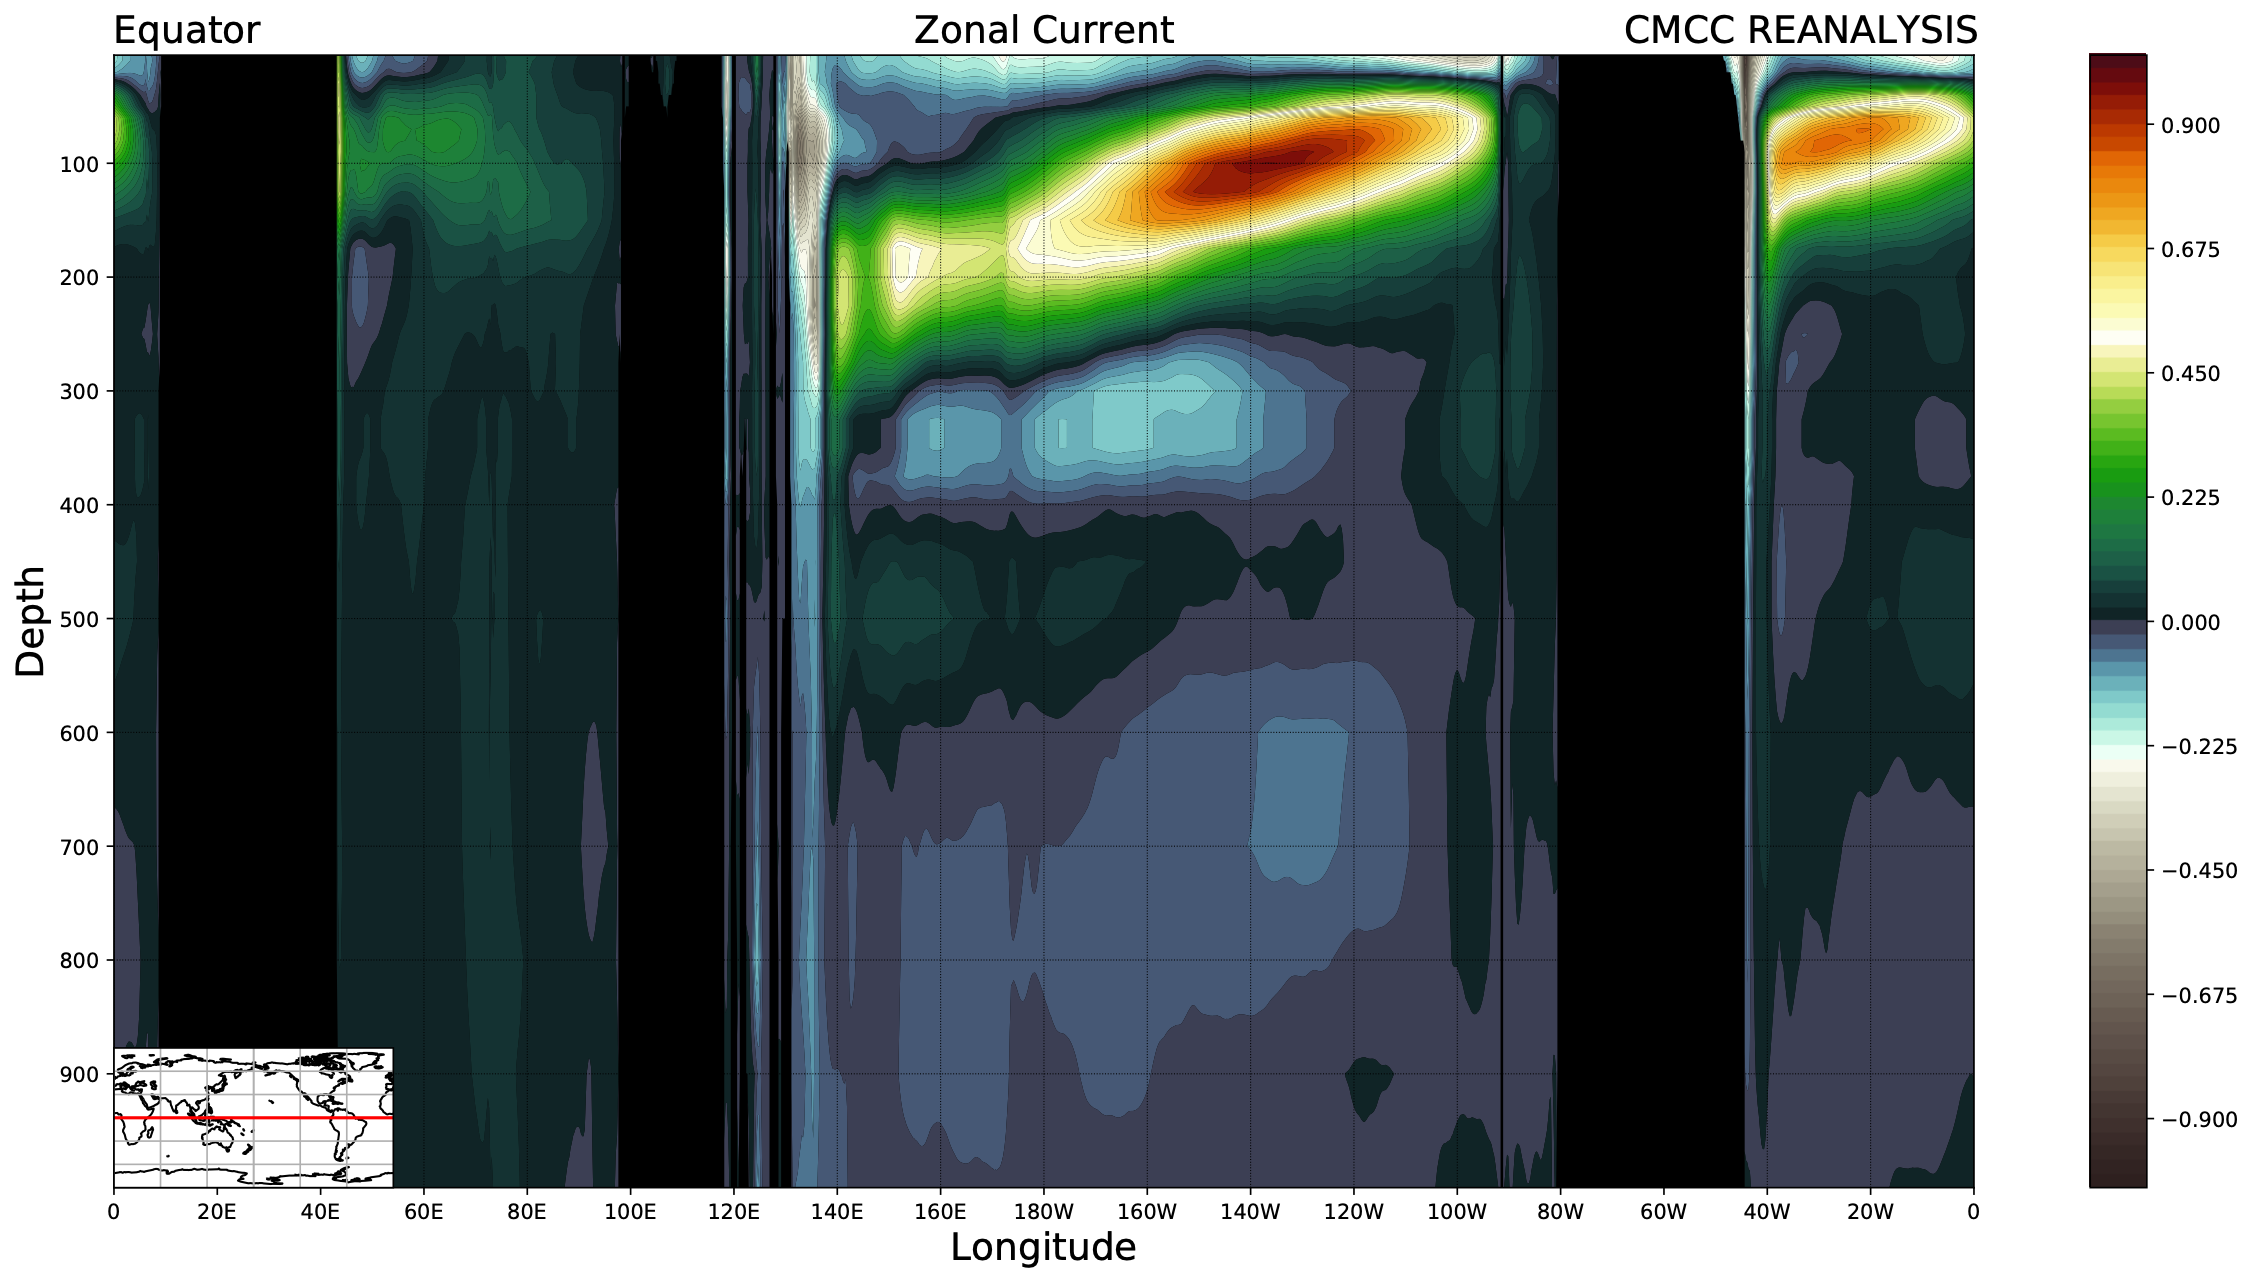
\includegraphics[width = 0.4 \textwidth]{upload/40image.png}
	\caption{Alternation of westerly and easterly currents} \label{fig:fig16}
\end{figure}

The equatorial Atlantic Ocean surface circulation (Figure 1.14). It is possible to see the easterly South Equatorial
Current that is straddling the Equator between 5S and 5N. The North
equatorial Countercurrent is westerly and it covers the area between 5N
and 10N, and the weaker North Equatorial Current is located at northern
latitudes. The equatorial flow is divergent and also in this case we can
presume the existence of upwelling at the Equator. A strong coastal
current is visible as the Guinea Current, in the Gulf of Guinea. The
South Equatorial Current feeds into the North Brazilian Current that
then flows northward along the South America coast, taking different
names as it finally emerges as the Caribbean Current in the Caribbean
sea.
\begin{figure}[htpb!]
	\centering
	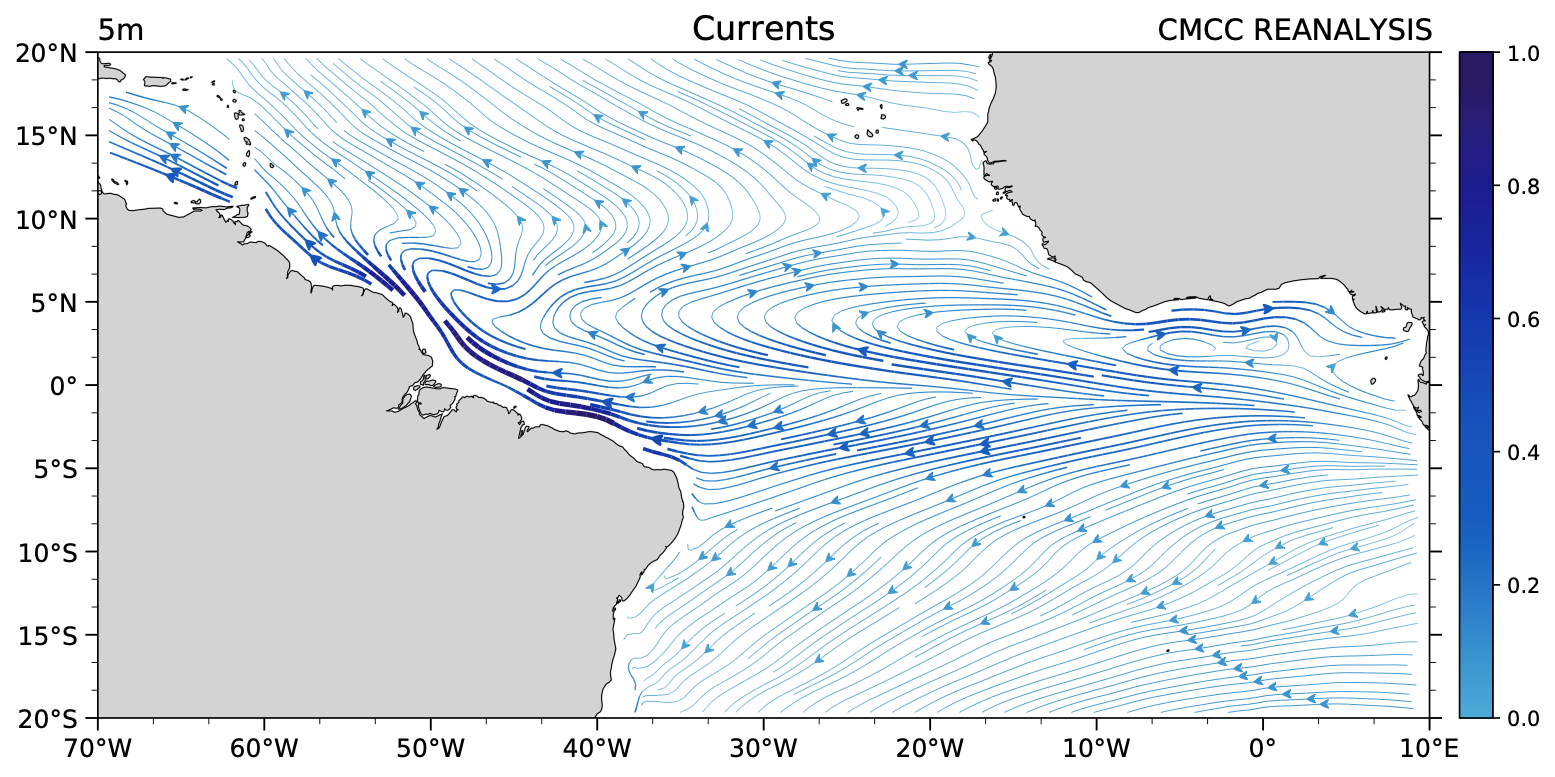
\includegraphics[width=0.45\linewidth]{upload/41image.png}\quad 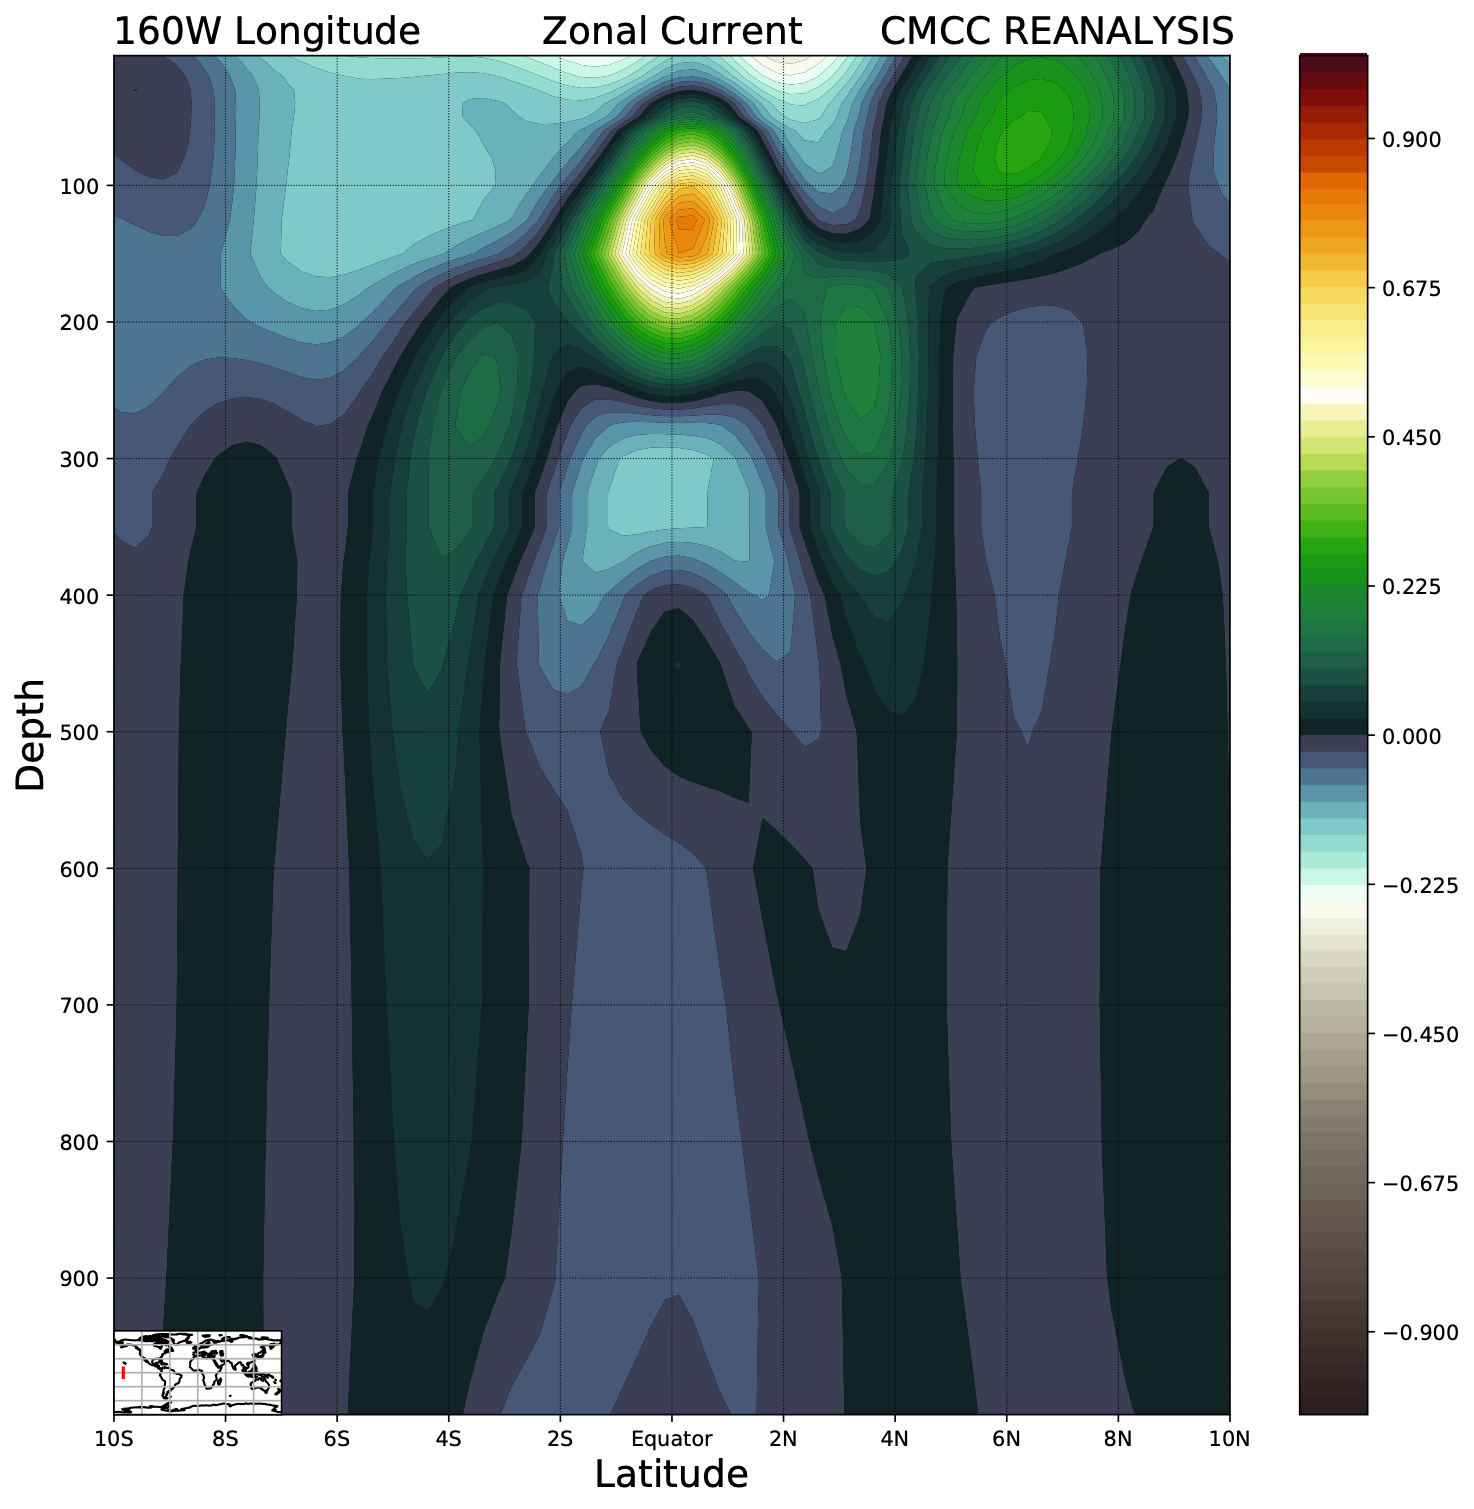
\includegraphics[width=0.3\linewidth]{upload/42.png}
	\caption{The equatorial Atlantic Ocean surface circulation and the structure of currents and undercurrents}
	\label{fig:fig17}
\end{figure}
A similar structure of alternating westerly and easterly undercurrents
exist also in the equatorial Atlantic (Figure 1.14), but it
is weaker and only the first westerly maximum is well visible. It is
also slanting towards the East, but the maximum is reached more towards
the western boundary of the basin with respect to the Pacific Ocean. The
deeper easterly jets are also much less weaker. The undercurrents jets
are essentially absent in the Indian Ocean.


\paragraph{The Gulf Stream}\label{the-gulf-stream}

The current system of the Gulf Stream is one of the major feature of the
global ocean circulation.


\subparagraph{The Kuroshio}\label{the-kuroshio}

The current system of the Kuroshio is one of the major features of the
global ocean circulation.


\begin{figure}[htpb!]
	\centering
	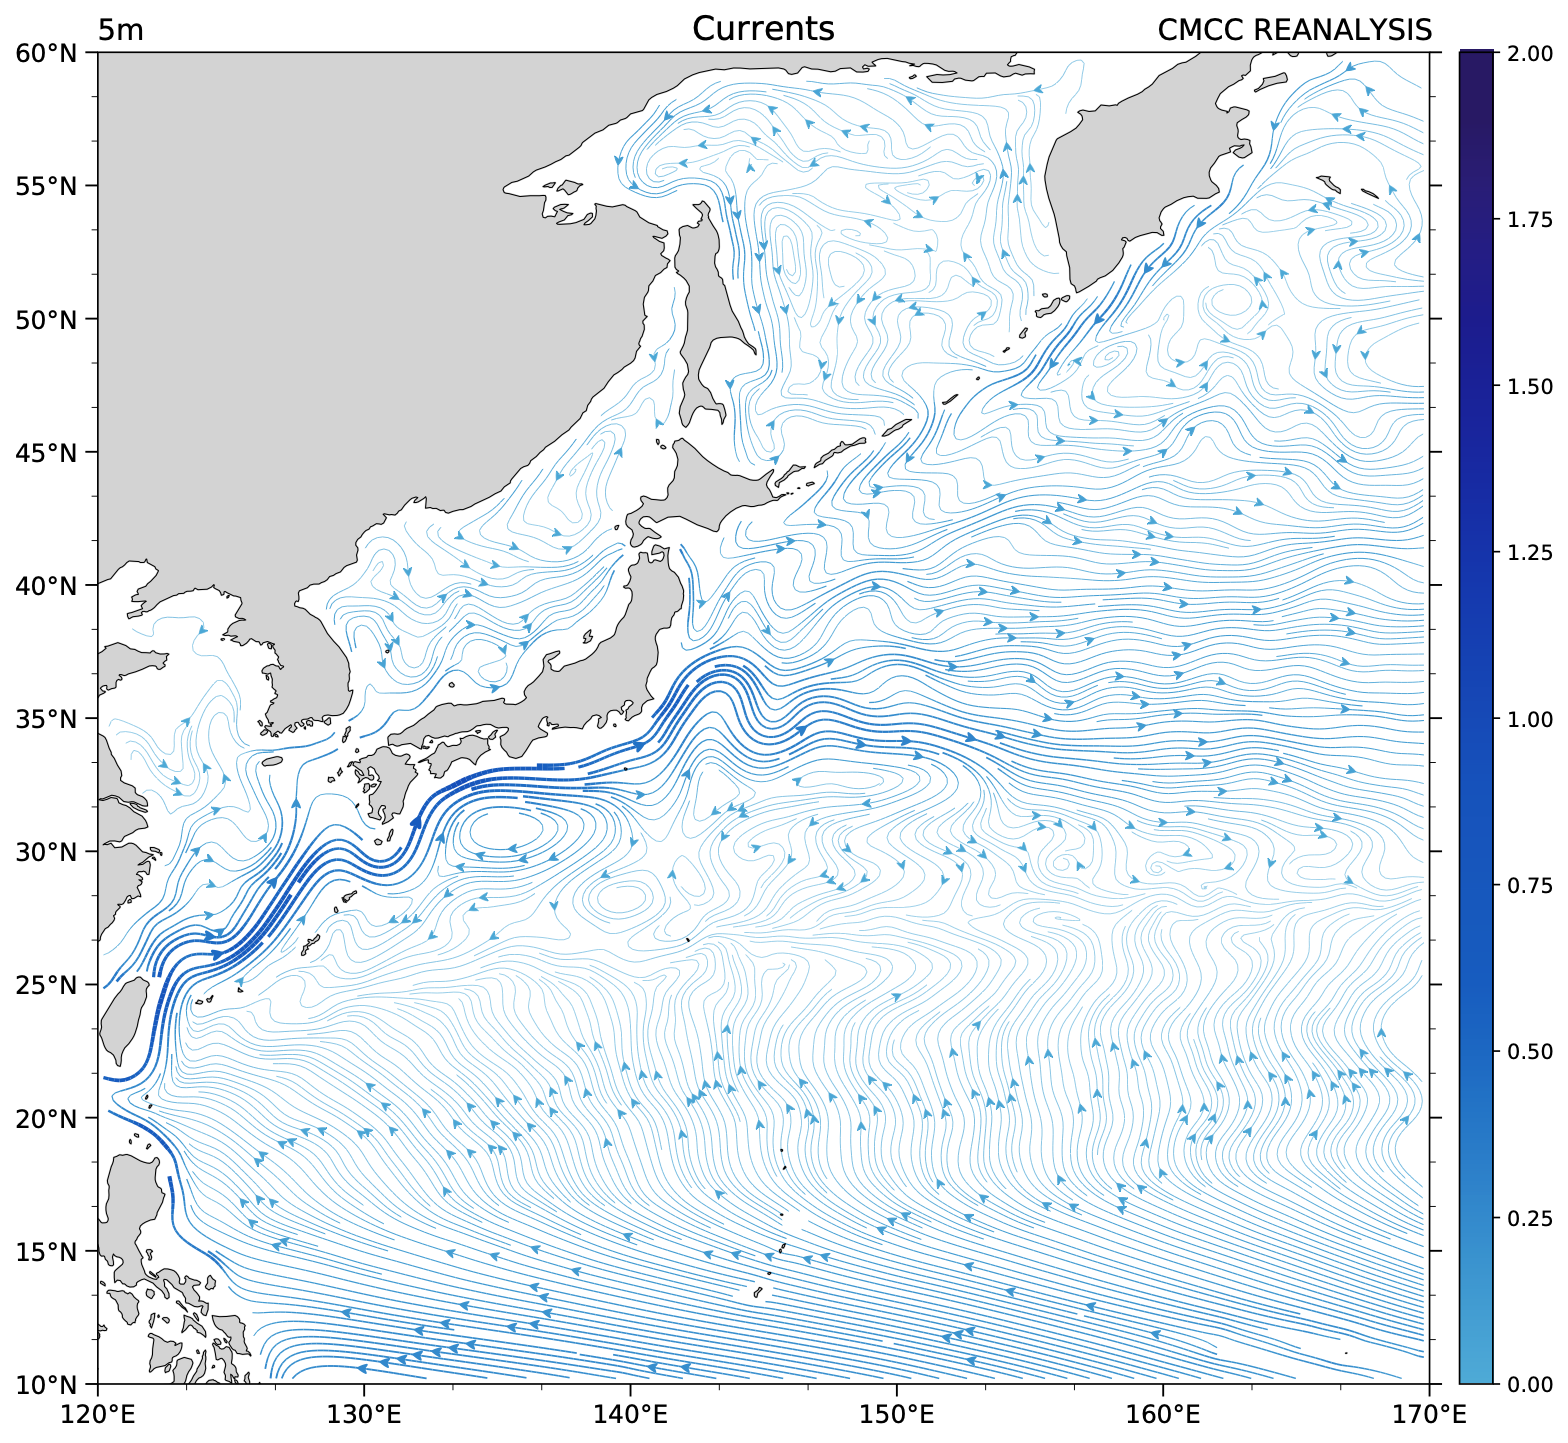
\includegraphics[width = 0.30 \textwidth]{upload/44.png}\quad 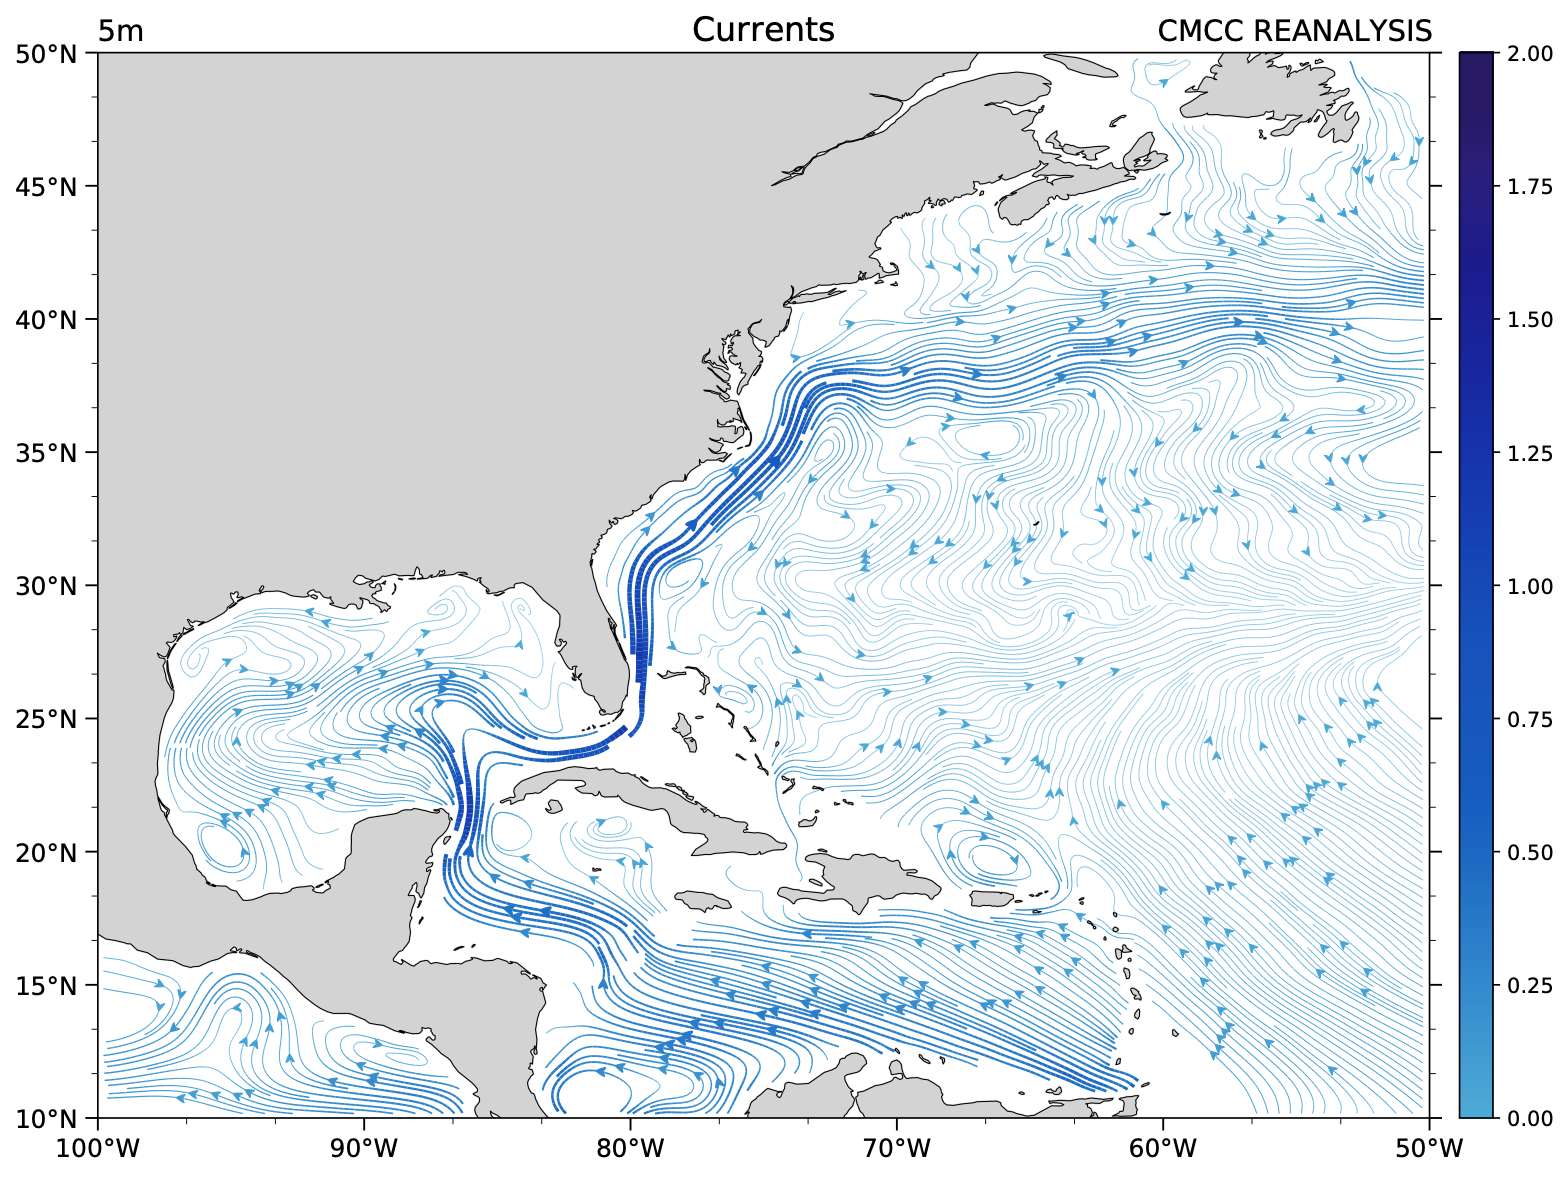
\includegraphics[width = 0.35\textwidth]{upload/43.png}
	\caption{The Kuroshio on the left and Gulf Stream on the right} \label{fig:}
\end{figure}

\begin{figure}[htpb!]
	\centering
	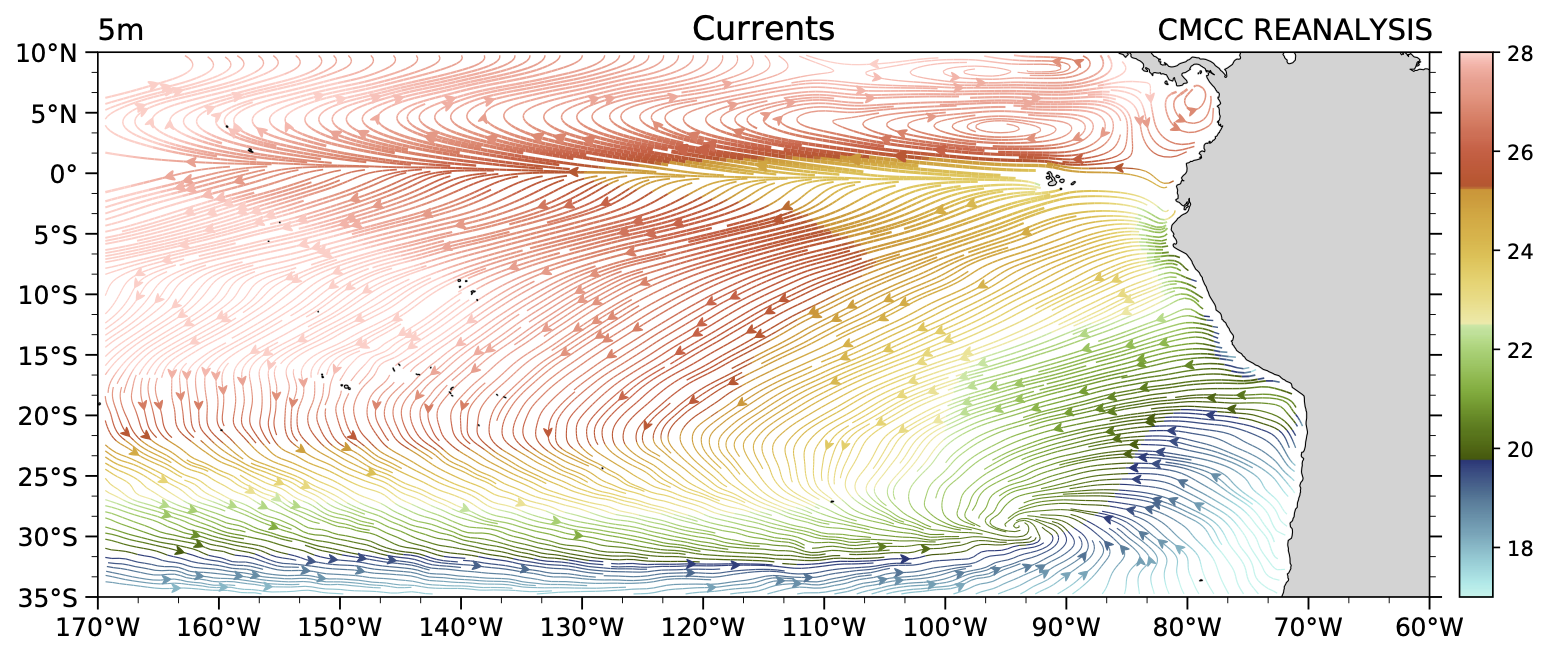
\includegraphics[width = 0.45 \textwidth]{upload/45.png}\quad 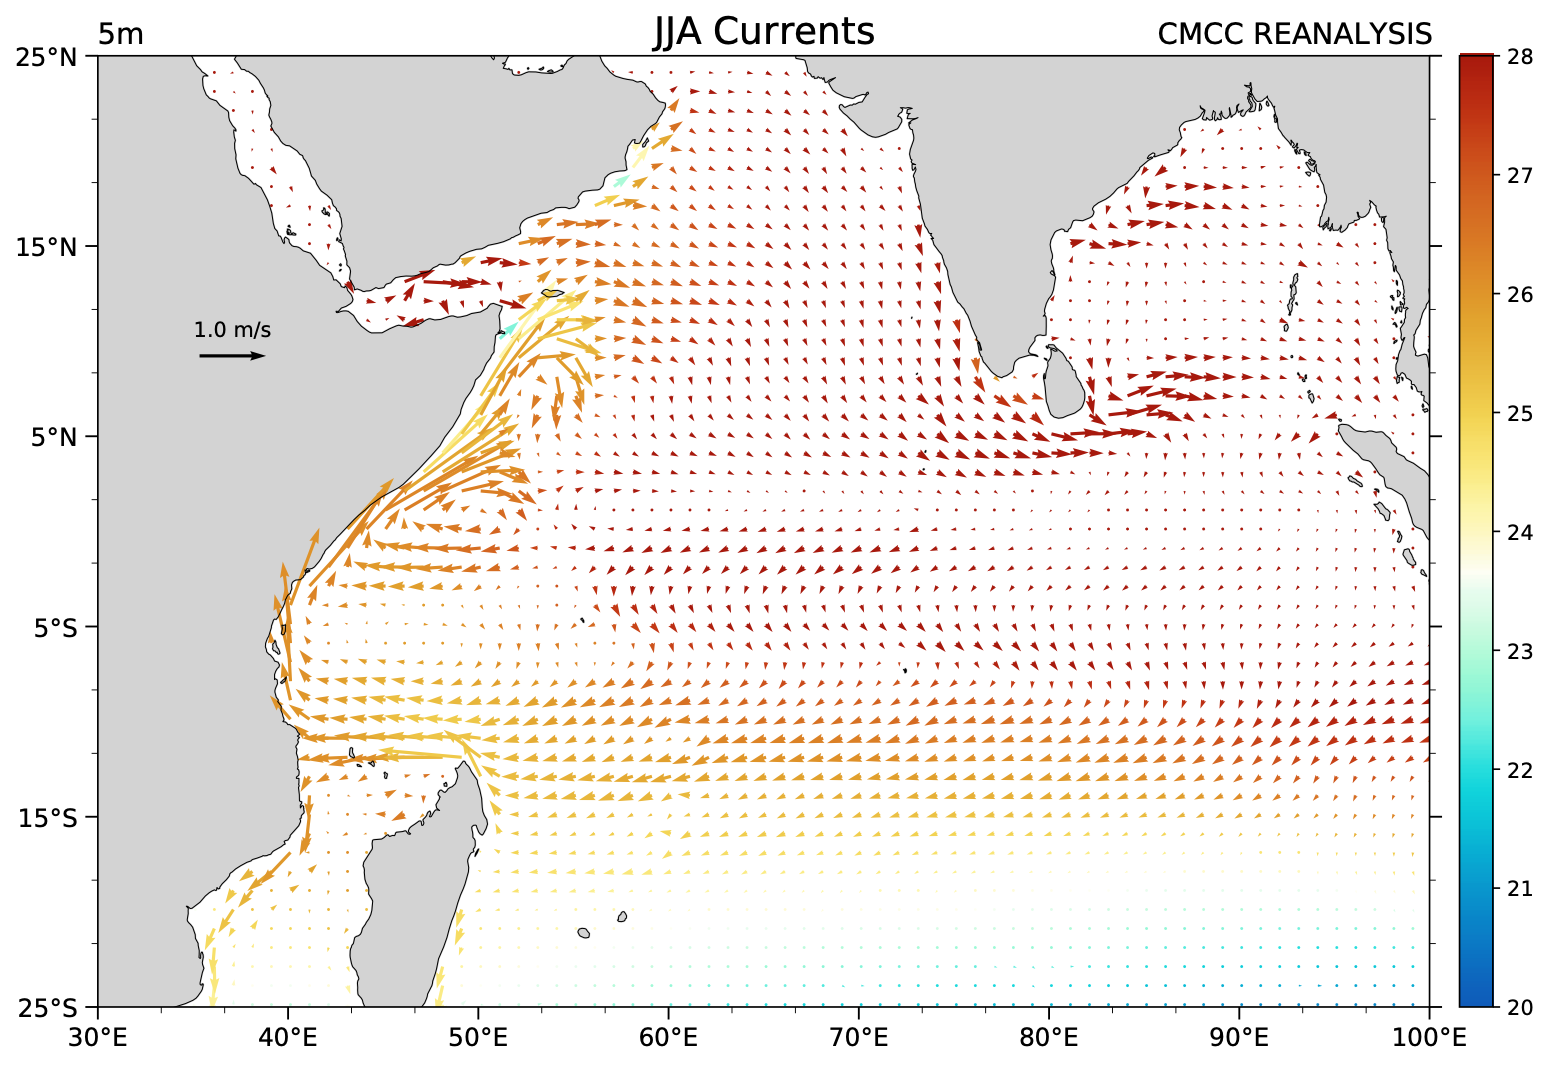
\includegraphics[width = 0.35\textwidth]{upload/46.png}
	\caption{The upwelling zones on the left and the Somali current on the right.} \label{fig:upwelzone}
\end{figure}




\section{Ice}
Sea ice covers about $7$\% of Earth's oceans and plays a critical role in the global climate system, acting as a barrier between the atmosphere and the ocean. It forms when seawater cools below its freezing point, creating ice floes that are often cracked and shifted by environmental forces. Despite its compact appearance, sea ice is dynamic and never fully covers open water areas due to constant movement and deformation. \\
In the Southern Hemisphere, sea ice extends seasonally from about $3$ million km\(^2\) in summer to $18$ million km² in winter, covering around $7$\% of the Southern Ocean at its peak. The ice can reach as far as $60°$S during winter, particularly in the Weddell and Ross Seas. However, it tends to be less compact compared to the Arctic, largely due to divergent winds and the influence of ocean currents. By contrast, in the Northern Hemisphere, sea ice ranges from $7$ million km\(^2\) in summer to $15$ million km² in winter, making up about $10$\% of the ocean area during its maximum extent. The Arctic Ocean forms the core region of sea ice, with thick polar caps and thinner ice in surrounding seas like the Bering Sea and the Sea of Okhotsk. Ice can also drift into the North Atlantic through the Labrador and Greenland seas.
The formation of sea ice depends on several factors. Salinity plays a crucial role, as higher salinity lowers the freezing point of seawater. In regions with salinity levels above $24.7$\%, convective mixing occurs as dense, salty water sinks, delaying the freezing process. Under calm conditions, supercooling can allow water to remain liquid below its freezing point until ice crystals form, which then accelerate the freezing of surrounding water. As the ice thickens, it insulates the ocean below, reducing heat loss and slowing further growth. \\
Sea ice melts during summer, particularly in the Arctic, where increased sunlight and prolonged daylight accelerate the process. Melting can occur at rates of about $40$ mm per day, with melt ponds and drainage channels forming on the surface. The loss of ice is further aided by tidal forces and storms, leading to disintegration near coastlines and open water areas. By late summer, much of the peripheral sea ice in the Arctic disappears, leaving only the central ice pack. \\
Sea ice properties vary greatly between the Arctic and Antarctic regions. In the Arctic, central ice thickness typically ranges from $2$ to $4$ meters, with thinner ice in peripheral seas ($0.5$ to $1$ meter). Antarctic icebergs are far larger, often exceeding $600$ meters in thickness. Ice density, generally between $880$ and $910$ kg/m\(^3\), allows it to float. The topography of sea ice includes ridges and rubble zones formed by colliding ice sheets, with some ridges extending $10$ to $15$ meters below the surface. \\
The movement of sea ice is also an important factor in ocean circulation and climate. In the Arctic, the Beaufort Gyre and the Transpolar Drift Stream transport ice across the Arctic Basin, eventually exiting through the Fram Strait into the North Atlantic. This ice contributes to cold currents like the East Greenland Current. In the Antarctic, ice drifts clockwise in the Weddell Sea, eventually melting in warmer waters and transporting freshwater to lower latitudes. \\
[0.15 cm]

Overall, sea ice is a vital component of Earth's climate system. It influences heat exchange between the ocean and atmosphere, regulates salinity and density in ocean waters, and contributes to the broader dynamics of polar and global ocean circulation. Its seasonal cycles and properties make it an essential focus for understanding climate change and its impacts.

\section{Interconnections between atmosphere, ocean and ice}
Important transfers of energy, mass, momentum occur between the oceans and the atmosphere and are greatly modified by the presence of sea ice.
\subsection{Atmosphere effect}
Wind forcing is a prime driver for upper ocean circulation and thereby impacts deep ocean circulation as well, and for sea ice thereby impacting its motions and location. In addition, air temperatures and moisture contribute to determining the energy fluxes across the interface between the atmosphere and surface, contributing to ice maintenance, growth and melt and to the temperature distribution in the ocean and water velocity.
Fridtjorf Nanse noted that sea ice does not drift in the direction of the wind but at an angle of $20-40°$ to the right due to the Earth’s rotation and speculated that the motions in the water beneath sea ice deviate even more; the motion of each water layer deviate slower and farther to the right to the layer above and Ekman proved it mathematically adding that these influence stops at a depth of about $200$ m.

\subsection{Ocean effect}
Ocean has a significant impact on the other two components. It is essentially a limitless moisture source and supplies the majority of atmospheric water vapor. The ocean land contrast exerts a major control over the distribution of evaporation over the global precipitation. The thermal inertia of the ocean results in a much lesser seasonal temperature range at the open ocean surface than at a land surface or a sea ice surface.
This creates a lesser atmospheric temperature range over open ocean than over land or sea ice, as cold winter air is warmed by the underlying ocean and warm summer air is cooled. %non ho capito fedeeeee
Since the ocean also absorbs a significant amount of the atmosphere’s carbon dioxide ($CO_2$), it also helps to slow the buildup of atmospheric $CO_2$. \\
[0.1 cm]
The oceans contribute significantly to the poleward transport of heat, by means of ocean currents. This transport influences the heat balances in both high and low latitudes and the average temperature gradient between the equator and the poles. The temperature distribution of the ocean surface is the prime determinant of the sea ice distribution, because, in general, ice forms where the water temperature has reached the freezing point. Similarly, the ocean salinity distribution is important to the formation of sea ice, because the salt content of the water affects the freezing temperature. Once ice is formed, warm currents entering an ice-covered region tend to melt the ice cover, and cold currents moving away from the ice region tend to carry ice with them.

\subsubsection{El Niño/Southern Oscillation (ENSO)}
This is an example of atmosphere/ocean interconnections one of the major large-scale patterns. The El Niño and Southern Oscillation phenomena were originally examined separately, before their close interconnection became apparent.\\
[0.1cm]
\textbf{El Niño} originally referred to a seasonal warming of the waters along the coast of Peru, frequently occurring shortly after Christmas. The term is now generally restricted to large-scale warming events, extending well into the central equatorial Pacific. The episodes can last many months, and do not necessarily begin near Christmas. \textbf{The Southern Oscillation}, characterized by consistent sea level pressure, temperature, and precipitation changes in the South Pacific, was first discussed by Walker who found an alternating pressure pattern involving the normal southeast Pacific high pressure and the low pressure region near the Indian Ocean and western Pacific regions. \\
[0,1cm]
\textit{Under normal conditions} (non–El Niño), there is a strong sea surface temperature difference between the warm western Pacific and the cooler eastern Pacific, caused by upwelling along South America's west coast driven by east-to-west trade winds. This setup creates a convection cycle where air rises over the warm western Pacific, leading to heavy rainfall, and sinks over the cooler eastern Pacific, forming an east-west Walker circulation.\\
\textit{During El Niño}, the trade winds weaken, reducing upwelling along the South American coast. This leads to warmer sea surface temperatures in the eastern Pacific, disrupting the temperature gradient. As a result, air rising and rainfall patterns shift eastward, cooling the western Pacific and causing significant climate effects. For example, the Indonesian-Australian region may experience drought, while wetter conditions occur farther east.
\begin{figure}[htpb]
	\centering
	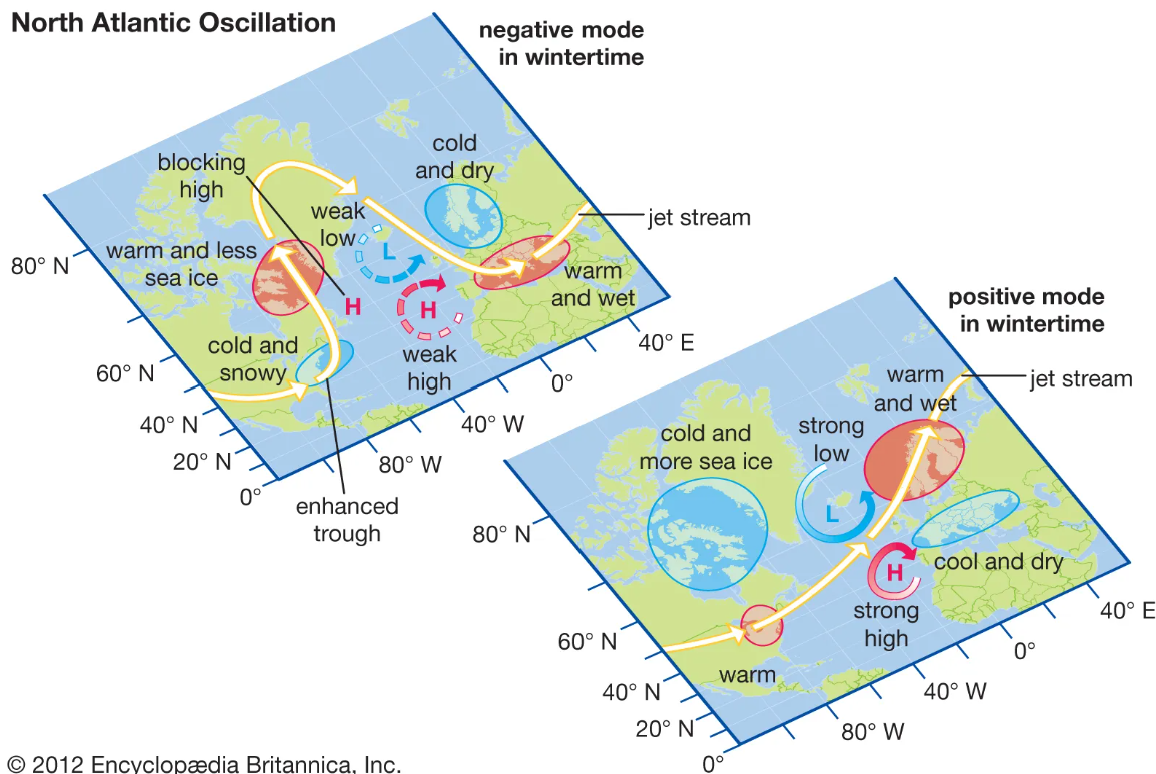
\includegraphics[width=0.5\linewidth]{upload/NAO.png}
	\caption{NAO}
	\label{fig:enter-label}
\end{figure}
\subsubsection{North Atlantic Oscillation (NAO)}
The North Atlantic Oscillation (NAO) is a pressure oscillation measured by the sea level pressure difference between Iceland and the Azores, reflecting the strength of the Icelandic low-pressure system and the Azores high-pressure system. (although sometimes it is indexed instead by the pressure difference between Newfoundland and Lisbon, Portugal, or between Iceland and Lisbon). It has both short-term and long-term variations, significantly affecting North Atlantic climate patterns. Positive NAO phases strengthen the Icelandic low pressure, resulting in colder winters in eastern North America, warmer and wetter conditions in western Europe, reduced sea ice near Greenland and Scandinavia, and increased sea ice in Baffin Bay and the Labrador Sea. \\
NAO impacts extend to global teleconnections, including influences on Russia, the Indian monsoon, and ocean temperatures. The positive NAO phase is associated with a tripolar sea surface temperature pattern: a cold anomaly in the subpolar North Atlantic, warm anomalies near Europe, and a cold subtropical anomaly near the Equator. The Gulf Stream further propagates these anomalies toward Europe, enabling atmospheric feedback and improving predictability of NAO patterns. The interaction between the ocean and the NAO remains a key area of research.



\subsection{Ice}
The presence of sea ice has numerous climatic consequences, influencing the temperature and circulation patterns of both the atmosphere and the oceans. Sea ice lessens the amount of solar radiation absorbed at the ocean's surface: only about $20–50$\% of the incident solar radiation is absorbed, the rest being reflected to space and is therefore lost, while without the ice, typically $85–95$\% is absorbed.
It serves as a strong insulator, restricting exchanges of heat from $10^2$ to $10^3 \,\,\text{Wm}^{-2}$  from the ocean to the atmosphere, to $10$ to $20 \,\,\text{Wm}^{-2}$;   mass, momentum, and chemical constituents between the ocean and atmosphere. \\
In winter, ice cover enhances polar cooling by increasing temperature gradients between the poles and the equator, intensifying atmospheric circulation. However, stronger circulation brings warm air into polar regions, reducing these gradients and creating a negative feedback, making the overall effect on atmospheric circulation uncertain. In summer, ice acts as a thermal insulator, reducing heat transfer from the atmosphere to the ocean. Its high albedo also reflects solar radiation, limiting heat absorption and increasing the net heat gain in polar oceans. These seasonal dynamics highlight the complex role of ice in the climate system.\\

Another aspect of the insulation is the lessened evaporative transfer to the atmosphere in the presence of ice cover, resulting in reduction of moisture available for cloud formation, rain and snow. \\
[0.1 cm]
The freezing and melting of sea ice influence seasonal and regional climates by moderating temperature extremes. Ice formation releases heat, while melting absorbs heat, facilitating a net equatorward transport of heat and salt from polar regions. During ice formation, salt is rejected into the underlying ocean, increasing the salinity and density of the mixed ocean layer, which can lead to deep convection and the formation of bottom water that drives global ocean circulation.
This process is most significant at the edges of ice packs, where winds create open water that freezes rapidly, enhancing local ice production. Approximately one-third of bottom water originates from ice formation along ice margins. These dynamics connect ice processes to global climate systems, influencing both local and large-scale ocean circulation.

\chapter{Fundamental Equations and processes}
\lastupdated{2024-12-13}{\chapterTwoEqsProcOverleaf}

\section{Fundamental Equations}
\subsection{Introduction\label{introduction}}

Sample citation of \cite{Richardson1922}.

The atmosphere is in motion and it is a continuous mixing and clashing
of vortices and structures, but when it is averaged over a long period
of time (fig.{\ref{fig:ERA5-wind200}}) it shows a remarkable simple structure.
The figure shows the wind at an approximate level of about 12km, that is
considered to be in the free atmosphere, far from the influence of the
ground. The circulation is a large vortex around the pole that shows
small oscillation in latitudes, especially pronounced over North America
and the Asian Pacific Coast. The flow is therefore predominantly in the
East-West direction, with a relatively small component in the meridional
direction. The \emph{circumpolar vortex} has been one of the first
structures to be recognized when plentiful observations of the upper air
flow became available, but it provided some of the intriguing questions
that drove the development of geophysical fluid dynamics to this time,
some of them have not been completely understood. What is maintaining
this peculiar circulation? Which factor determines the amplitude and
location of the undulations in meridional direction? Some of these
question will be addressed in these chapter.

\begin{figure}[htpb]
	\centering
	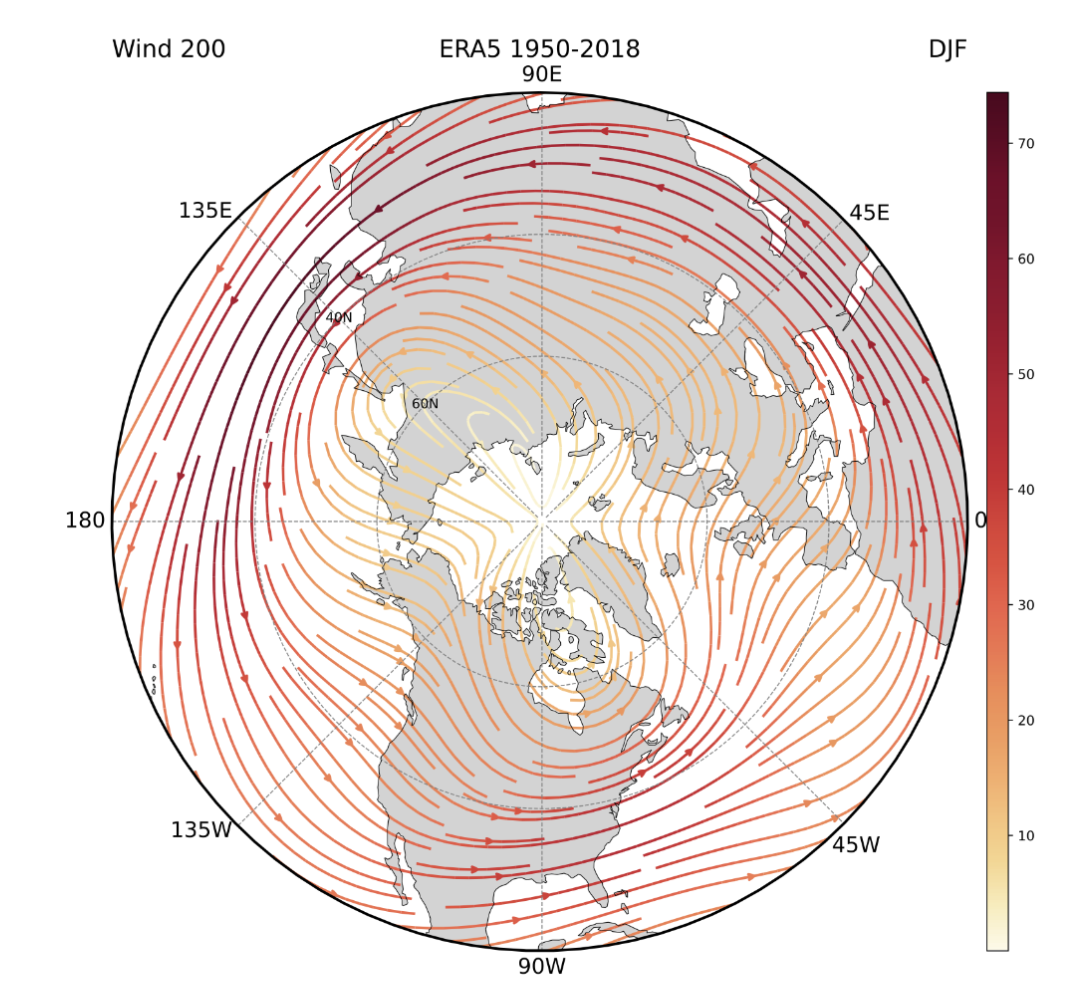
\includegraphics[width=0.35\linewidth]{upload/Screenshot 2024-11-18 114256.png}
	\caption{ERA5-wind 200}
	\label{fig:ERA5-wind200}
\end{figure}


\subsection{Coordinate systems}\label{coordinate-systems}

\paragraph{Spherical Coordinates}\label{spherical-coordinates}

The most commonly used coordinate system for the analysis of the
atmosphere and the oceans is a spherical coordinate system attached to
the rotating Earth (Fig. \ref{fig:coordinate system3d} ). The spherical coordinates are
slightly different from the usual mathematical ones as the latitude is
measured from the equator and therefore it can take negative values. The
longitude is running west to east.

The longitude is also known as the ``zonal'' direction whereas the
latitude is also known as the "meridional" direction. Winds are
identified by the direction they are coming from, so a "westerly" wind
is coming \emph{from} the West and an "easterly" wind is coming from the
East.

This coordinate system is rotating with the Earth and therefore it
generates force terms in any dynamical equation expressed in this system
of coordinate, the Coriolis terms.

\begin{figure}[htpb]
	\centering
	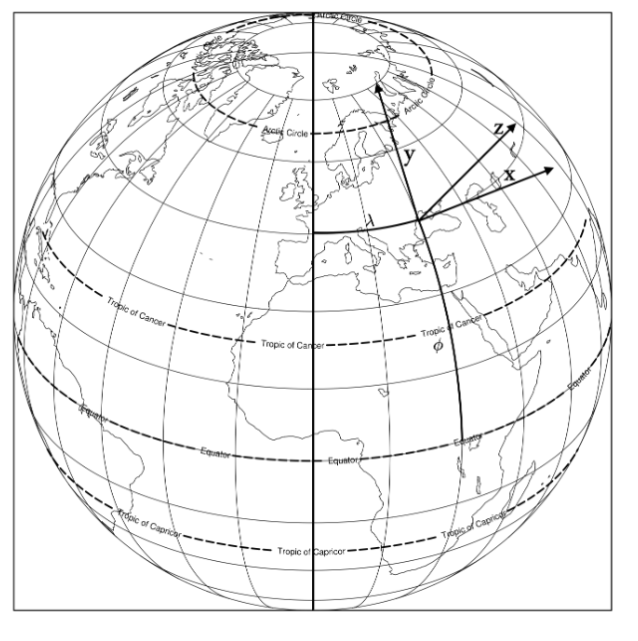
\includegraphics[width=0.4\linewidth]{upload/Screenshot 2024-11-18 114156.png}
	\caption{Coordinate system}
	\label{fig:coordinate system3d}
\end{figure}

\subsubsection{The Beta-plane}\label{the-beta-plane}

It is sometimes convenient to shift coordinate system if the latitudinal
extension of the motion is not too great with respect to the motion
parameters as they are expressed in the adimensional numbers. When this
is possible, a tangent coordinate system is applied at a specific
latitude \(\phi_0\) and the resultant Cartesian coordinates system is
called the \(\beta\)-plane. Usually symbols \((x,y)\) are used in this
case for the zonal and meridional coordinate. In the \(\beta\)-plane the
planetary vorticity \(f\) is linearized as \(f=f_0 + \beta y\), where
\(\beta = \frac{\partial f}{\partial y}({\phi_0})\).

\subsubsection{Advective derivative}\label{Sec:Adv}

To describe the governing equation of the atmosphere and eventually of
the ocean we have to understand how we write the rate of change with
time of this fluid. This problem was solved by considering the fact that
the rate of change in the fluid cannot be seen as rate of change with
respect to a fixed system of coordinate because the system is moving
with the fluid itself. Therefore, first we have to find a way to
describe the change taking into account the moving system of
restaurants. These can be done by using a concept developed in the 19th
century by Euler that is called "advective derivative" that can be
obtained from a total derivative of the property,

\[\frac{d \phi}{dt} = \frac{\partial \phi}{\partial t} + \frac{\partial x}{\partial t}\frac{\partial \phi}{\partial x} + \frac{\partial y}{\partial t}\frac{\partial \phi}{\partial y}+\frac{\partial z}{\partial t}\frac{\partial \phi}{\partial z} = \frac{\partial \phi}{\partial t} + \mathbf{v}\cdot\nabla\phi\]

and so it can be defined as

\[\frac{D \varphi}{Dt} =\frac{\partial \varphi}{\partial t} + \mathbf{v}\cdot\nabla\varphi\]

in this way the moving fluid can be described by derivatives with
respect the "fixed" coordinate system, i.e. the Eulerian description.
The alternative description of the observer moving with fluid is known
as the "Lagrangian" description.



\subsection{Equation of motion} %this section comes from lecture6
The motion of a physical system is governed by conservation laws: conservation of momentum, mass and energy. The conservation of momentum equation will identify the forces acting on the system. The conservation of energy will identify the processes capable of changing the energy of the system, i.e. thermodynamical processes.
The equation governing the motion of the atmosphere can be written as:
\[
	\begin{aligned}
		 & \frac{D u}{Dt} -\frac{uv \tan{\phi}}{r} +  \frac{uw}{r} = -\frac{1}{\rho r \cos{\phi}}\frac{\partial p}{\partial \lambda} + fv - \hat{f}w + F_\lambda \\
		 & \frac{D v}{Dt} -\frac{u^2 \tan{\phi}}{r} +  \frac{vw}{r} = -\frac{1}{\rho r }\frac{\partial p}{\partial \phi} - fu  + F_\phi                          \\
		 & \frac{D w}{Dt} -\frac{u^2+v^2}{r} = -\frac{1}{\rho }\frac{\partial p}{\partial z} -g +\hat{f}u + F_z                                                  \\
	\end{aligned}\]

the \(f=2\Omega \sin{\phi}\) and \(\hat{f} = 2\Omega\cos{\phi}\) terms arise from the rotating spherical coordinate system that we have chosen, other terms are generated by the spherical geometry. Some of them are small and traditionally they can be neglected, so that we arrive at the system

\[\begin{aligned}
		 & \frac{D u}{Dt} - v\left(f +  \frac{u \tan{\phi}}{a}\right)  = -\frac{1}{\rho a \cos{\phi}}\frac{\partial p}{\partial \lambda}   + F_\lambda \\
		 & \frac{D v}{Dt} + u\left( f + \frac{u \tan{\phi}}{a}\right)  = -\frac{1}{\rho a}\frac{\partial p}{\partial \phi}  + F_\phi                   \\
		 & \frac{D w}{Dt}  = -\frac{1}{\rho }\frac{\partial p}{\partial z} -g  + F_z                                                                   \\
	\end{aligned}\]

where we have also used the \emph{Shallowness Approximation} by assuming \(r = a +z \approx a\), where \(a\) is the Earth radius.

However the advective derivative must be expressed in spherical cordinates

\[\frac{D }{Dt} = \frac{\partial }{\partial t} + \frac{u}{a\cos{\phi}}\frac{\partial }{\partial \lambda} +\frac{v}{a}\frac{\partial }{\partial \phi} + w\frac{\partial }{\partial z}\]

so that the velocity components are

\[\begin{aligned}
		 & u = a\cos{\phi\frac{\partial \lambda}{\partial t}} \\
		 & v = a \frac{\partial \phi}{\partial t}             \\
		 & w = \frac{\partial z}{\partial t}
	\end{aligned}\]

These equations govern the mechanical behaviour of the atmosphere, and we will see in a different form, also of the ocean. There three forces in action: pressure gradient, rotation via the Coriolis force and gravity.

The equation are not complete,we have three equation but five variables, so we need to find the missing relations. We are using the basic conservation principles, the latter equations describe the conservation
of momentum, we can exploit the conservation of mass. The mass of the fluid must be conserved locally, because there are now sinks or sources in the atmosphere itself, so we want to write the mass of a volume of
atmosphere fixed in space as

\[M = \int_V  \rho \,dV\]

the mass in the volume can only change if there is a flux of mass at surface \(S\),

\[\frac{\partial }{\partial t} \int_V  \rho \,dV = -\int_S \rho\mathbf{v}\cdot n \, dS\]

using the divergence theorem however we have

\[\frac{\partial }{\partial t} \int_V  \rho \,dV = -\int_V \nabla\cdot(\rho\mathbf{v}) \,dV\]

because the volume is not changing with time we can bring the derivative inside the integral and we get

\[\int_V  \frac{\partial \rho}{\partial t}+\nabla\cdot(\rho\mathbf{v}) \,dV = 0\]

but the volume is arbitrary, so it must be that

\[\frac{\partial \rho}{\partial t}+\nabla\cdot(\rho\mathbf{v}) = 0\]

is valid locally.

We have still at our disposal the conservation of thermodynamical energy and so we can also use the first law of thermodynamics for a gas, that is a statement of internal energy, where $C_v$ is the specific heat for air at constant volume and $T$ is the temperature in Kelvins.

\[c_v\frac{D T}{Dt} = -p\frac{D }{Dt}\left(\frac{1}{\rho}\right)+ Q\]

where we included the temperature and heating/cooling term \(Q\) (which is the net heat gain or loss to the external sources, for example the solar insolation, heating or cooling due to long wave radiation, latent heating due to condansation of water vapor into liquid water, and sensible heating due to conduction and convection). The state variable are then linked by the state equation

\[p = \rho R T\]

where \(R\) is the gas constant for dry air.

We can use the equation of state to write the energy equation (or the temperature equation) in a different form,

\[c_v\frac{D T}{Dt} = -p\frac{D }{Dt}\left(\frac{R T}{p}\right)+ Q = -R\frac{D T}{Dt} + \frac{RT}{p}\frac{D p}{Dt} + Q\]

yielding the alternative forms ( since \(c_p = c_v +R\)),

\[c_p\frac{D T}{Dt}  - \frac{1}{\rho}\frac{D p}{Dt} = Q\]
For many purpose atmospheric and oceanic motions can be considered essentially adiabatic. However, for climate studies, the assumption of exclusively adiabatic processes is not appropriate since the amount of heat added or lost to a unit volume of air or water over a long period of time can be substantial. For adiabatic processes \(Q=0\):

\[\begin{aligned}
		 & c_p\frac{D T}{Dt}  - \frac{1}{\rho}\frac{D p}{Dt} = 0        \\
		 & \frac{c_p}{T}\frac{D T}{Dt} -\frac{R}{p}\frac{D p}{Dt} = 0   \\
		 & \frac{D }{Dt}\log{T} - \frac{R}{c_p}\frac{D }{Dt}\log{p} = 0
	\end{aligned}\]

integrating it we get

\[\log{T/T_0} - \log{\left(\frac{p}{p_0}\right)^{R/c_p}} = \text{const}\]

or

\[\frac{T}{T_0}\left(\frac{p_0}{p}\right)^{R/c_p} = \text{const}\]

so the quantity, known as \emph{potential temperature}

\[\theta = T\left(\frac{p_0}{p}\right)^{R/c_p}\]

is conserved in adiabatic processes and the thermodynamics equation can be written as

\[\frac{D \theta}{Dt} = Q\]

\paragraph{Hydrostatic balance.}
Under the action of gravity the vertical component of the pressure
gradient force balances the action of gravity, resulting in very small
vertical acceleration

\[\frac{\partial p}{\partial z} =  -g \rho\]

then if we take the vertical derivative of the eq. \texttt{Eq:logT}

\[\frac{1}{T_0}\frac{d T}{dz}\left(\frac{p_0}{p}\right)^{R/c_p} -\frac{p_0}{p^2}\frac{R}{c_p}\frac{T}{T_0}\left(\frac{p_0}{p}\right)^{R/c_p-1}\frac{d p}{dz} = 0\]

simplifying

\[\frac{d T}{dz} -\frac{p_0}{p^2}\frac{R}{c_p}T\left(\frac{p_0}{p}\right)^{-1}\frac{d p}{dz} = 0\]

or

\[\frac{d T}{dz} -\frac{1}{p}\frac{R}{c_p}T\frac{d p}{dz} = \frac{d T}{dz} +g\rho\frac{1}{p}\frac{R}{c_p}T = 0\]

but using the equation of state

\[\frac{d T}{dz} = -\frac{g}{c_p}\]

that gives how the temperature change with height under adiabatic
conditions and when the hydrostatic balance is valid. This is known as
the \emph{adiabatic lapse rate}. If I assume:
$$C_p= 1000;   \frac{-g}{C_p} =10°C/km$$
the temperature must drops linearly with height.

If we integrate over height $z$, assuming isothermal atmosphere, we get an exponential trend over density $\rho$ and pressure $p$, which drops with height (because of the perfect gas law):
$$p(z)=p_0 e^{\frac{-RT}{g}z}$$
\paragraph{Geostrophic balance.} Geostrophic balance is the balance between Coriolis Force and the horizontal component of the pressure gradient force.
\begin{figure}
	\centering
	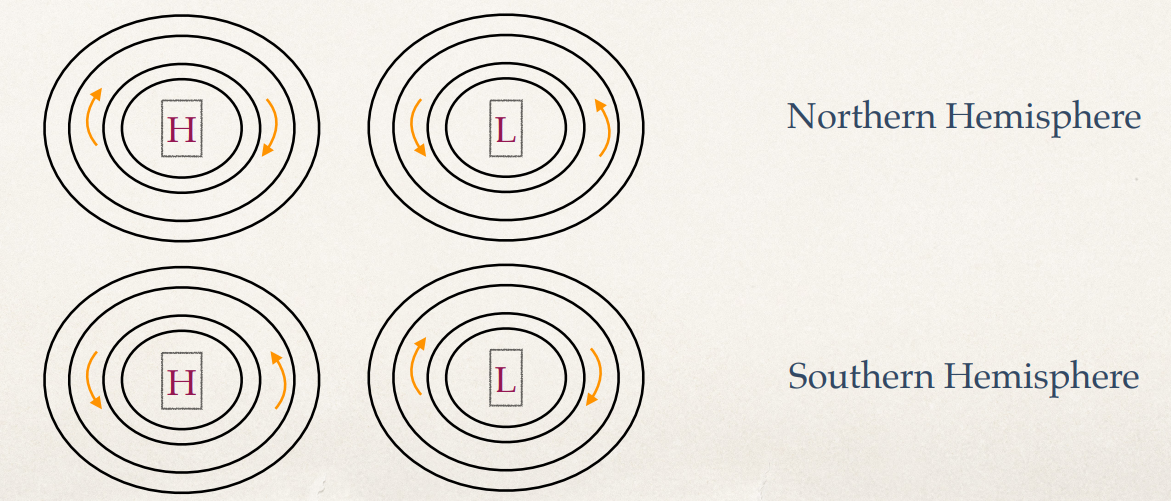
\includegraphics[width=0.5\linewidth]{upload/Screenshot 2024-11-20 195919.png}
	\caption{Geostrophic balance}

\end{figure}
The pressure gradient force (PGF) pushes air or water from high pressure to low pressure. The Coriolis force deflects the motion to the right in the Northern Hemisphere and to the left in the Southern Hemisphere. In geostrophic balance, these forces are equal in magnitude and opposite in direction. The geostrophic balance assumes the flow is steady and does not accelerate, so it neglects the effects of inertia. This balance is most accurate for large-scale motions (e.g., planetary or synoptic scales) where friction and other forces are negligible. Vertical motions are typically much smaller than horizontal motions and are neglected in geostrophic balance.

In geostrophic balance:
\begin{itemize}
	\item Air or water flows parallel to the isobars (lines of constant pressure) or contours of constant geopotential height.
	\item The speed of the geostrophic flow increases with stronger pressure gradients (closer isobars).
\end{itemize}
However, on small scales (e.g., tornadoes, boundary layers), friction and other forces become important, so geostrophic balance is less accurate. Near the Equator, The Coriolis parameter ($f$) approaches zero, making the geostrophic balance invalid.

\paragraph{Advective derivative in rotating coordinates.} A vector in spherical coordinates is:
$$\mathbf{u}=\hat{i}u+\hat{j}v+\hat{k}w$$
but the unit vectors move in a rotating frame, so the advective derivative of a vector is given by:
\begin{equation}\label{eq.adv der in rotating}
	\frac{Du}{Dt}=\frac{Du}{Dt}\hat{i}+\frac{Dv}{Dt}\hat{j}+\frac{Dw}{Dt}\hat{k}+u\frac{D\hat{i}}{Dt}+v\frac{D\hat{j}}{Dt}+w\frac{D\hat{k}}{Dt}
\end{equation}
\paragraph{Coriolis Factors}
The Coriolis forces derives from the conservation of angular momentum.
$$\frac{d}{dt}\left(R_A(\Omega R_A+u)\right)=0$$
or
$$2\Omega R_A\frac{dR_A}{dt}+u\frac{dR_A}{dt}+R_A\frac{du}{dt}=0$$
rearraging
$$\frac{du}{dt}=(2\Omega R_A+u)\frac{dR_A}{dt}$$
\begin{figure}[h!]
	\centering
	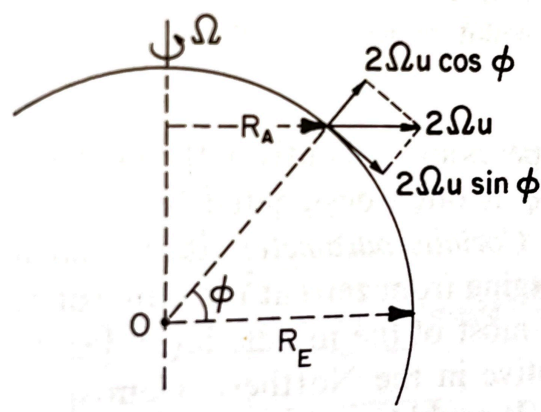
\includegraphics[width=0.35\linewidth]{upload/Screenshot 2024-11-21 164025.png}
	\caption{Coriolis factors}
	\label{fig:coriolis}
\end{figure}
The Coriolis components then are $2\Omega\sin\phi$ and $2\Omega\cos\phi$. For the horizontal and vertical components respectively:
$f=2\Omega\sin\phi$.

\subsection{Summary of fundamental
	equations-}\label{summary-of-fundamental-equations}

Summarizing our discussion, the fundamental equation that describe the
motion of the atmosphere are considered in the following approximations:
\begin{itemize}
	\item Hydrostatic approximation
	\item Shallow fluid approximation. The vertical coordinate $r$ is sustituted by $a+z(a>>z)$ except in differentiation
	\item Neglecting metric terms involving vertical velocity $w$
\end{itemize}
The first approximation is independent, the second and the third must be applied together. These primitive (non hydrostatic) equations are:
\[\begin{aligned}
		 & \frac{D u}{Dt} - v\left(f +  \frac{u \tan{\phi}}{a}\right)  = -\frac{1}{ a \cos{\phi}}\frac{1}{\rho}\frac{\partial p}{\partial \lambda}   + F_\lambda                                                     \\
		 & \frac{D v}{Dt} + u\left( f + \frac{u \tan{\phi}}{a}\right)  = -\frac{1}{a}\frac{1}{\rho}\frac{\partial p}{\partial \phi}  + F_\phi                                                                        \\
		 & \frac{D w}{Dt}  = -\frac{1}{\rho }\frac{\partial p}{\partial z} -g  + F_z \label{Eq:PrimEq}                                                                                                               \\
		 & \frac{D \theta}{Dt} = Q                                                                                                                                                                                   \\
		 & \frac{\partial \rho}{\partial t}+\frac{1}{a\cos{\phi}}\left[ \frac{\partial }{\partial \lambda}(\rho u) + \frac{\partial }{\partial \phi}(rv\cos{\phi} )\right] +\frac{\partial }{\partial z}(\rho w) = 0 \\
		 & p = \rho R T
	\end{aligned}\]

where we have used the divergence in spherical coordinates.

These equations are still not closed because we will need to express the heating/cooling term \(Q\) and the friction terms \(F\) as a function of the state variables. This will require a theory of the processes that drive them. Where \(R=287.052874 J \quad \text{kg}^{-1} \text{K}^{-1}\) is the gas constant for dry air and \(c_p = 1.005\) is the specific heat at constant pressure, \(c_v = 0.718\) is the specific heat at constant volume, \(\kappa = \frac{R}{c_p}\) and \(\gamma=c_p/c_v\) is their ratio.

\subsection{Simplified equations-}\label{summary-of-fundamental-equations}

For theoretical and idealized studies the set of equation projected on the \(\beta\)-plane is also used. The $\beta$-plane approximation is a simplified model used in geophysical fluid dynamics to account the variation of the Coriolis parameter $f$ with latitude, in this approximation $f$ is linearized around a reference latitude such that $f\approx f_0+\beta y$ with $y=a(\phi-\phi_0)$ is the northward displacement from the reference latitude. With the $\beta$-plane approximation, no rotation, no sphericity, neglecting the meridional coordinates , the equations become:

\[\begin{aligned}
		 & \frac{D u}{Dt} - fv  = -\frac{1}{\rho}\frac{\partial p}{\partial x}   + F_x \\
		 & \frac{D v}{Dt} + fu = -\frac{1}{\rho}\frac{\partial p}{\partial y}  + F_y   \\
		 & \frac{D w}{Dt}  = -\frac{1}{\rho }\frac{\partial p}{\partial z} -g  + F_z   \\
		 & \frac{D \theta}{Dt} = Q                                                     \\
		 & \frac{\partial \rho}{\partial t}+\nabla\cdot(\rho\mathbf{v}) = 0            \\
		 & p = \rho R T
	\end{aligned}\]

and the gradient operator is the cartesian operator

\[\nabla = \frac{\partial }{\partial x} + \frac{\partial }{\partial y} + \frac{\partial }{\partial z}\]

and the advective derivative is then

\[\frac{D }{Dt} = \frac{\partial }{\partial t} + u\frac{\partial }{\partial x} + v\frac{\partial }{\partial y} + w\frac{\partial }{\partial z}\]

The first set of fundamental equations that we encounter is the conservation of Momentum (\textbf{Navier-Stokes equations)}.\\
The Navier-Stokes equations describe the motion of fluid substances like air and water. They account for forces due to pressure, viscosity, and external forces such as gravity. This set of equations is key to understanding how winds, ocean currents, and other flows evolve due to internal and external forces. In a rotating frame of reference, specifically describing the motion of a fluid (e.g. the atmosphere or ocean currents) the principal equation can be declined in the different directions: longitude, latitude and vertical directions.

The left-hand side of the equations begins with material derivative of the velocity components ($u$ in the east-west direction, associated with longitude; $v$ north-south velocity component, associated with latitude, $w$ is the vertical velocity component).
The material derivative includes both the local rate of change and the advection (transport) of the velocity. This term tells us how the velocity of a fluid parcel changes over time, taking into account both temporal changes and the movement of the parcel.

The second term on the left represents the Coriolis force and the centrifugal force in the rotating reference frame of the Earth. $f$ is the Coriolis parameter, which depends on the latitude $\phi$ and is given by $f=2\Omega\sin\phi$ where $\Omega$ is the angular velocity of the Earth and $\phi$ is the latitude. The Coriolis force is proportional to the velocity and acts perpendicular to the motion of the fluid, deflecting the fluid in different directions depending on the hemisphere.

On the right side of the equations we find the pressure gradient force in the longitudinal (first) and latitudinal (second) directions, which drives fluid motion due to differences in pressure. The terms $F_{\lambda}$, $F_{\phi}$ and $F_{z}$ represent an additional force term that could represent any other forces acting on the fluid parcel in the longitudinal, latitudinal and vertical direction. It might include friction, external forces, or any other model-specific forces not accounted for in the other terms.\\

Let's now focus on them one by one.
\begin{equation}
	\frac{Du}{Dt}-v\left(f+\frac{u\tan\phi}{a}\right)=-\frac{1}{a\cos\phi}\frac{1}{\rho}\frac{\partial p}{\partial\lambda}+F_{\lambda}
\end{equation}
The term $\frac{u\tan\phi}{a}$ accounts for the centrifugal force resulting from the Earth's rotation. Here, $u$ is the east-west velocity, $\phi$ is the latitude, and $a$ is the Earth's radius. The centrifugal force is stronger near the equator, and this term adjusts the Coriolis effect to account for that.
$\frac{\partial p}{\partial\lambda}$ is the derivative of pressure with respect to longitude ($\lambda$), indicating how pressure changes as you move east or west. The term $a\cos\phi$ accounts for the spherical geometry of the Earth and the fact that distances between lines of longitude vary with latitude (they are widest at the Equator and shrink towards the poles). This term describes the acceleration due to the horizontal pressure gradient in the longitudinal direction, with the pressure gradient force causing flow from regions of higher to lower pressure.
\begin{equation}
	\frac{Dv}{Dt}+u\left(f+\frac{v\tan\phi}{a}\right)=-\frac{1}{a}\frac{1}{\rho}\frac{\partial p}{\partial\phi}+F_{\phi}
\end{equation}
The term $\frac{v\tan\phi}{a}$ is the centrifugal force term in the north-south direction, considering Earth's curvature. $\frac{p}{\phi}$ represents the pressure gradient in the latitude direction, and it drives motion from high to low pressure.


Note that the Coriolis term arises due to the rotation of the Earth, which introduces an apparent force in a rotating reference frame. This term depends explicitly on the latitude because of how the Earth's rotation affects the direction and magnitude of the Coriolis effect at different points on the Earth's surface. The Coriolis force explicitly depends on the sine of the latitude, as the projection of $\Omega$ onto the local horizontal plane is $\Omega\sin\phi$ (the latitude $\phi$ determines the angle between the Earth's rotational axis and the local vertical. $\Omega$ is the angular velocity vector of Earth's rotation, it points along the axis of rotation (towards the North Pole). At the Equator $\phi=0°$ the Coriolis effect is perpendicular to $\Omega$ and has a max horizontal effect. At the poles ($\phi=\pm 90°$) the effect aligns with $\Omega$, and only the vertical motion is affected.

In the \textbf{vertical direction}:
%check if these are correct
\begin{equation}
	\frac{Dw}{Dt}=-\frac{1}{\rho}\frac{\partial p}{\partial z}-g+F_z
\end{equation}
While the Coriolis force primarily affects horizontal motion, the vertical component of the Coriolis force is negligible because $\Omega$ is nearly parallel to the vertical axis in most regions. In rotating systems like the atmosphere or oceans, vertical Coriolis terms are often ignored. $g$ acts downward and opposes upward motion.
\\


The equation
\begin{equation}
	\frac{D\theta}{Dt}=Q
\end{equation}

says that the rate of change of $\theta$ (the material derivative) experienced by a fluid parcel moving through space is equal to the source term $Q$. This equation describes the rate of change of a scalar quantity (like temperature or moisture) \textbf{for a fluid parcel} moving through space. The term $Q$ could represent a source of energy or mass, such as heat from the sun or moisture added by evaporation. In the context of a weather or climate model, this would represent how temperature (or another variable) changes as the air parcel moves and as energy is gained or lost.
This equation is a general form for describing the time evolution of a scalar quantity (like T or moisture) in a moving fluid, where the change in that quantity is driven by external sources or sinks.
\\



The \textbf{conservation of mass} or \textbf{continuity equation }ensures that the mass is conserved in the system. For the atmosphere or the ocean, it expresses how the density of air or water changes over time due to processes like flow and diffusion.
\begin{equation}
	\frac{\partial\rho}{\partial t}+\nabla\cdot(\rho\vec{v})=0
\end{equation}
$\nabla\cdot(\rho\vec{v})$ represents the divergence of the mass flux, which accounts for the movement of the mass.
\\
The last one is the equation of state for atmospheric or oceanic models links pressure, density and temperature of the fluid. The \textbf{ideal gas law} is typically used:
\begin{equation}
	p=\rho RT
\end{equation}

\subsection{Linear solutions}
We look for solution that describe small oscillation away from a basic state, in this case assumed in hydrostatic balance with constant wind of velocity $u$, and I'm looking at deviation from this basic state:
\begin{equation}
	\frac{\partial p_0}{\partial z}=-g\rho_0=-\frac{gp_0}{RT_0}
\end{equation}
With the further assumption of isotherm atmosphere we can integrate to get:
\begin{equation}
	p_0(z)=p_Re^{-z/H}
\end{equation}
and $H=\frac{RT_0}{g}$ is the scale height. \\


As we have seen, the primitive equations are a system of nonlinear partial differential equations governing fluid motion on a rotating sphere. These include momentum equations, continuity (mass conservation), thermodynamic equations and the equation of state. Since solving the full nonlinear system is often impractical, the system is linearized to analyze small deviations (or perturbations) from a reference state (steady flow or a state of rest). Assume the flow can be separated into a basic state and a perturbation:
\begin{align*}
	u=u_0+u'                \\
	v=v_0+v'                \\
	\theta=\theta_0+\theta' \\
	p=p_0+p'
\end{align*}
The resulting linearized primitive equations describe how perturbations evolve over time and space (linear equations are obtained for the prime variables neglecting all terms quadratic in perturbation).
For instance, the pressure gradient becomes:
\begin{equation}
	\frac{1}{\rho_0+\rho'}\nabla(p_0+p')+g\hat{k}\approx\frac{1}{\rho_0+\rho'}\nabla p'+g\hat{k}=\frac{1}{\rho_0}\frac{1}{1+\frac{\rho'}{\rho_0}}\nabla p'+g\hat{k}=\frac{1}{\rho_0}\nabla p'+g\hat{k}
\end{equation}
and the potential temperature:
$$
	\theta=T\left(\frac{p_R}{p}\right)^k=\frac{p_R^k}{R}\frac{p^{1-k}}{\rho}\approx\theta_0\left[1+\frac{1}{\gamma}\left(\frac{p'}{p_0}\right)-\frac{\rho'}{\rho_0}\right]
$$
hence,
\begin{equation}
	\frac{\theta'}{\theta_0}=\frac{1}{\gamma}\frac{p'}{p_0}-\frac{\rho'}{\rho_0}
\end{equation}
with $\gamma=\frac{c_p}{c_v}$, $k=\frac{R}{c_v}$, $R=c_p-c_v$.

\subsection{Waves}
The linearized system often supports wave-like solutions. These solutions arise naturally due to the restoring forces in the equations, such as:
\begin{itemize}
	\item Pressure gradient drives the oscillations through compressibility or buoyancy
	\item Coriolis force introduces rotational effects leading to inertial and planetary waves
	\item Gravity acts as a restoring force for vertical displacement, driving internal gravity waves.
\end{itemize}

We take the equations for perturbation:
\begin{align*}
	\frac{\partial u}{\partial t}+U\frac{\partial u}{\partial x}+\frac{1}{\rho_0}\frac{\partial p}{\partial x}=0                                                              \\
	\frac{\partial w}{\partial t}+U\frac{\partial w}{\partial x}+\frac{1}{\rho_0}\frac{\partial p}{\partial z}+g\frac{\rho}{\rho_0}=0                                         \\
	\frac{\partial\rho}{\partial t}+U\frac{\partial\rho}{\partial x}+w\frac{\partial\rho_0}{\partial z}+\rho_0(\frac{\partial u}{\partial x}+\frac{\partial w}{\partial z})=0 \\
	\frac{\partial\theta}{\partial t}+U\frac{\partial\theta}{\partial x}+w\frac{\partial\theta_0}{\partial z}=0                                                               \\
	\frac{\theta}{\theta_0}+\frac{\rho}{\rho_0}+\frac{1}{\gamma}\frac{p}{p_0}=0
\end{align*}

%slides 24-29 LEC6 non le ha molto cagate
Basically to find solutions, assume the perturbations take the form of plane waves:
$$\mathbf{u'}(x,t)=\hat{\mathbf{u}}e^{i(\mathbf{k}\cdot\mathbf{x}-\omega t)}$$
where $\mathbf{\hat{u}}$ is the amplitude of the perturbation, $\mathbf{k}$ is the wavevector, $\omega$ the angular velocity. Substituing this kind of wave into the linearized equations leads to a dispersion relation, which relates $\omega$ to $\mathbf{k}$ and the physical parameters of the system (Coriolis, ...).
The perturbation equations link the restoring forces to wave properties:
\begin{enumerate}
	\item The momentum equations describe how velocity perturbations interact with pressure gradients and Coriolis forces.
	\item The continuity equation ensures mass conservation, connecting velocity and density perturbations.
	\item The thermodynamic equation relates temperature, pressure and density perturbations
\end{enumerate}
Imposing the hydrostatic approximation from the beginning would mean putting to zero from the start the time derivative of $w$ in the momentum equation in the vertical. This basically is equivalent to say that we are removing the explicit dependence of the vertical velocity on time and therefore we will get waves similar to the Boussinesq approximation. The hydrostatic approximation eliminates vertical propagating sound waves, but the Lamb waves still exists.


\section{Homogeneous flows}\label{homogeneous-flows}

\begin{figure}[htpb]
	\centering
	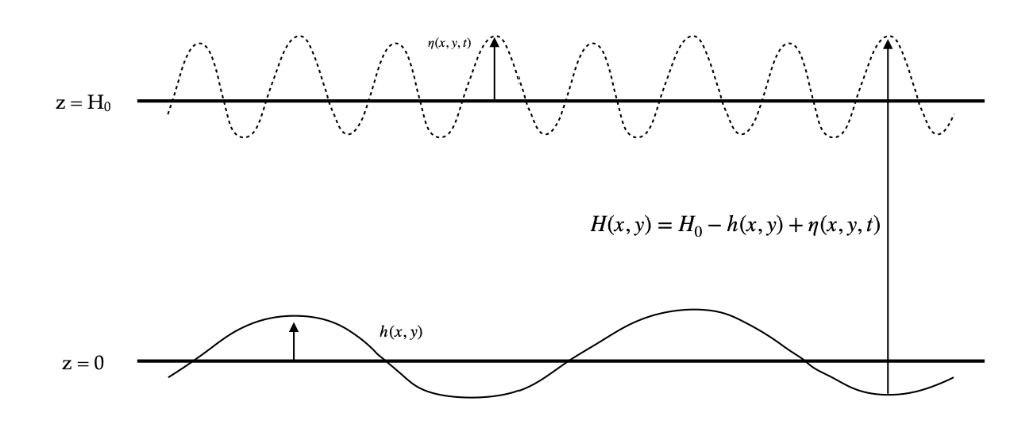
\includegraphics[width=0.5\linewidth]{upload/image732864.png}
	\caption{Homogeneous flow}
	\label{fig:homo}
\end{figure}



The motion of the atmosphere is most appropriately described by
three-dimensional equations that describes the horizontal and vertical
motion of the fluid, however a lot can be understood by considering a
simpler system that consider the motion of a free surface of a inviscid,
homogeneous and incompressible fluid. These equations are variously
referred to as one-level primitive equations or the \textit{shallow water
	equations}.

The system is described in Fig. \ref{fig:homo}, it is an homogenous
layer of fluid covering the entire spherical planet. We have included a
bottom topography \(h(x,y)\) and a deformation of the free surface
\(\eta(x,y)\). The convention is such positive deformation of the
surface are increasing the depth of the fluid, whereas positive
deformation of the bottom are decreasing it.

We have introduced here cartesian coordinates \((x,y)\) such that
\(dx \approx a \cos\theta d \lambda\) and \(dy \approx a d\theta\), we
will also define \(f= 2\Omega \sin\theta\), then the incompressible
equations of motion can be written as

\[
	\begin{aligned}
		\frac{\partial u}{\partial t} & = -u \frac{\partial u}{\partial x} -v \frac{\partial u}{\partial y} + f v -\frac{1}{\rho}\frac{\partial p}{\partial x} \\
		\frac{\partial v}{\partial t} & = -u \frac{\partial v}{\partial x} -v \frac{\partial v}{\partial y} - f u -\frac{1}{\rho}\frac{\partial p}{\partial y} \\
		\frac{\partial w}{\partial t} & = -u \frac{\partial w}{\partial x} -v \frac{\partial w}{\partial y} + g -\frac{1}{\rho}\frac{\partial p}{\partial z}   \\
		                              & \frac{\partial u}{\partial x} + \frac{\partial v}{\partial y} + \frac{\partial w}{\partial z} = 0
	\end{aligned}
\]

If the aspect ratio \(\delta \approx H/L\) is small then hydrostatic
balance is maintained to order \(\delta^2\) and so

\[\frac{\partial p}{\partial z} = - \rho g + O(\delta^2)\]

because the density is constant we can integrate it from 0 to \(z\) and
get

\[p = -\rho g (H_0+ \eta -z) + p_0\]

where we have used the boundary condition at the top
\(p(x,y,H_0 +\eta) = p_0\).

The horizontal pressure gradients are independent of \(z\)

\[\begin{aligned}
		\frac{\partial p}{\partial x} = \rho g \frac{\partial \eta}{\partial x} \\
		\frac{\partial p}{\partial y} = \rho g \frac{\partial \eta}{\partial y}
	\end{aligned}\]

because the horizontal accelerations are independent of z, than also the
velocities are independent of z, if they are so at the beginning. This
is in fact a consequence of the Taylor-Proudman theorem applied to a
homogeneous fluid. We can then write the horizontal momentum equations

\[\begin{aligned}
		\frac{\partial u}{\partial t} & = -u \frac{\partial u}{\partial x} -v \frac{\partial u}{\partial y} + f v -g\frac{\partial \eta}{\partial x} \\
		\frac{\partial v}{\partial t} & = -u \frac{\partial v}{\partial x} -v \frac{\partial v}{\partial y} - f u -g\frac{\partial \eta}{\partial y} \\
	\end{aligned}\]

Because \(u\) and \(v\) are independent of \(z\) allows us to integrate
vertically the divergence equation from the surface \(h(x,y)\) to an
height \(z\)

\[w(x,y,z,t) = -z\left(\frac{\partial u}{\partial x} + \frac{\partial v}{\partial y}\right) + \omega(x,y,t)\]

The kinematic condition for the bottom can be written as

\[\frac{D }{Dt}{(z-h)} = 0\]

or

\[w(x,y,h,t) =  u\frac{\partial h}{\partial x} + v\frac{\partial h}{\partial y}\]

so the function \(\omega\) is

\[\omega(x,y,t) = u\frac{\partial h}{\partial x} + v\frac{\partial h}{\partial y} + h \left(\frac{\partial u}{\partial x} + \frac{\partial v}{\partial y}\right)\]

then the vertical velocity can be written as

\[w(x,y,z,t) = (h-z)\left(\frac{\partial u}{\partial x} + \frac{\partial v}{\partial y}\right) + u\frac{\partial h}{\partial x} + v\frac{\partial h}{\partial y}\]

Using now the kinematic boundary condition at the top (\(z=H_0+\eta\))

\[w(x,y,H_0+\eta,t) = \left(\frac{\partial }{\partial t} + u\frac{\partial }{\partial x} + v\frac{\partial }{\partial y}\right)(H_0+\eta)\]

combining the last two equation we get an equation for the height

\[\frac{\partial \eta}{\partial t} + \frac{\partial }{\partial x}(H_0+\eta -h)u + \frac{\partial }{\partial y}(H_0+\eta -h)v = 0\]

and so we can now write the complete equations, introducing the total
depth of the fluid \(H=H_0+\eta -h\):

\[\begin{aligned}
		\frac{\partial u}{\partial t} & = -u \frac{\partial u}{\partial x} -v \frac{\partial u}{\partial y} + f v -g\frac{\partial H}{\partial x} \\
		\frac{\partial v}{\partial t} & = -u \frac{\partial v}{\partial x} -v \frac{\partial v}{\partial y} - f u -g\frac{\partial H}{\partial y} \\
		\frac{\partial H}{\partial t} & = - \frac{\partial (u H)}{\partial x} - \frac{\partial (v H)}{\partial y}                                 \\
	\end{aligned}\]
These equations are written in the approximation of no friction, molecular or turbulent; $w<<u$, from a scale analysis of $$\frac{\partial u}{\partial x}+\frac{\partial v}{\partial y}=-\frac{\partial w}{\partial z}$$
Linearizing around a state of rest, constant rotation:
\begin{align*}
	\frac{\partial u}{\partial t}-fv=-g\frac{\partial\eta}{\partial x} \\
	\frac{\partial v}{\partial t}+fv=-g\frac{\partial\eta}{\partial y} \\
	\frac{\partial\eta}{\partial t}=-H_0\left(\frac{\partial u}{\partial x}+\frac{\partial v}{\partial y}\right)
\end{align*}
the solutions are, respectively:
\begin{align*}
	u(x,y,t)=\text{Re}\left[\tilde{u}\sin(ly)e^{i(kx-\omega t)}\right] \\
	v(x,y,t)=\text{Re}\left[\tilde{v}\sin(ly)e^{i(kx-\omega t)}\right] \\
	\eta(x,y,t)=\text{Re}\left[\tilde{\eta}\sin(ly)e^{i(kx-\omega t)}\right]
\end{align*}
two modes\footnote{mode in this context refers to a specific solution or pattern of motion that satisfies the governing equations of the flow, under certain boudaries or initial conditions.}, a stationary mode and a gravity mode (Poincare' modes): $\omega=0$ and $\omega^2=f^2+gH_0(k^2+l^2)$


\subsection{\texorpdfstring{The vorticity equation on the
		\(\beta\)-plane}{The vorticity equation on the \textbackslash beta-plane}}\label{the-vorticity-equation-on-the-beta-plane}

The spherical geometry maybe cumbersome without adding much the
conceptual discussions, so it may be convenient to introduce Cartesian
coordinates \((x,y)\) such that \(dx \approx a \cos\theta d \lambda\)
and \(dy \approx a d\theta\), we will also define
\(f= 2\Omega \sin\theta\), then we obtain equation formally identical to
the Cartesian equation described previously

\[\begin{aligned}
		\frac{\partial u}{\partial t} & = -u \frac{\partial u}{\partial x} -v \frac{\partial u}{\partial y} + f v -g\frac{\partial \eta}{\partial x} \\
		\frac{\partial v}{\partial t} & = -u \frac{\partial v}{\partial x} -v \frac{\partial v}{\partial y} - f u -g\frac{\partial \eta}{\partial y} \\
		                              & \frac{\partial u}{\partial x}+\frac{\partial v}{\partial y} = 0                                              \\
	\end{aligned}\]

where we have kept the pressure terms, though they are zero in this case
($h$ is a constant) as a placeholder. In vector notation (all vectors are
two-dimensional)

\[\frac{\partial \mathbf{v}}{\partial t} = - (\mathbf{v} \cdot \nabla)\mathbf{v} - f(\hat{k}\times \mathbf{v}) - \nabla \eta\]

using the vector identity\footnote{For a general vector $\mathbf{A}$: \[\frac{1}{2}\nabla(A\cdot A) = (A \cdot\nabla)A + A\times(\nabla\times A)\]}


\[\frac{1}{2}\nabla(\mathbf{v}\cdot \mathbf{v}) = (\mathbf{v} \cdot\nabla)\mathbf{v} + \mathbf{v}\times(\nabla\times \mathbf{v})\]
so substituting in the equation

\begin{equation}\label{eq.21}
	\frac{\partial \mathbf{v}}{\partial t} = -(\zeta + f) \hat{k}\times \mathbf{v} -\nabla(\eta+\frac{1}{2}|\mathbf{v}^2|)
\end{equation}

(for 2-dimensional flows \(\nabla \times \mathbf{v} = \zeta \hat{k}\)).

and to express more clearly the components

\[\begin{aligned}
		\frac{\partial u}{\partial t} & = (\zeta +f) v -\frac{\partial }{\partial x}(\eta+\frac{1}{2}|\mathbf{v}^2|)  \\
		\frac{\partial v}{\partial t} & = -(\zeta +f) u -\frac{\partial }{\partial y}(\eta+\frac{1}{2}|\mathbf{v}^2|)
	\end{aligned}\]

By taking the curl of eq.\ref{eq.21} we obtain an equation for the vorticity (as it will be discussed in Sec.\ref{Sec:models on the sphere}:

\[\begin{aligned}
		\frac{\partial \zeta}{\partial t} & = -\frac{\partial }{\partial x}(\zeta +f) u -\frac{\partial }{\partial y}(\zeta +f) v                                                                                          \\
		                                  & -\frac{\partial }{\partial x} \frac{\partial }{\partial y}(p+\frac{1}{2}|\mathbf{v}^2|) +\frac{\partial }{\partial y}\frac{\partial }{\partial x}(p+\frac{1}{2}|\mathbf{v}^2|) \\
		                                  & =  -\frac{\partial }{\partial x}(\zeta +f) u -\frac{\partial }{\partial y}(\zeta +f) v = -\mathbf{v}\cdot\nabla(\zeta +f)
	\end{aligned}\]

where we have used the non divergence condition
\(\frac{\partial u}{\partial x}+\frac{\partial v}{\partial y}=0\) in the
last step. Once again, this is the equation for the conservation of
total vorticity where we can see that the relative vorticity is a sort
of additional Coriolis effect (or alternatively that the Coriolis term
is a source of vorticity). Because of the $\beta$-plane $f=f_0+\beta y$:
\begin{equation}\label{Barotropic equation}
	\frac{\partial\zeta}{\partial t}=-u\frac{\partial\zeta}{\partial x}-v\frac{\partial\zeta}{\partial y}-\beta v
\end{equation}
that is the non-divergent barotropic vorticity equation. And the potential vorticity:
\begin{equation}\label{eq.potential vorticity}
	\frac{D}{Dt}(\zeta +f)=0
\end{equation}

\(f= 2\Omega \sin(\theta)\) is the Coriolis coefficient, that is the
vertical component of the Earth planetary vorticity.

In the new coordinates \((x,y)\) for longitude and latitude, the
streamfunction and the vorticity then are

\[u=-\frac{\partial \psi}{\partial y}\qquad v=\frac{\partial \psi}{\partial x} \qquad
	\zeta = \frac{\partial x}{\partial x} -\frac{\partial u}{\partial y}=\nabla^2\psi\]

introducing the Jacobian operator

\[J(A,B) = \frac{\partial A}{\partial x}\frac{\partial B}{\partial y} - \frac{\partial A}{\partial y}\frac{\partial B}{\partial x}\]

we obtain a single equation for the streamfunction

\[\frac{\partial }{\partial t}\nabla^2\psi  + J(\psi, \nabla^2\psi +f_0 + \beta y) = 0\]
that represents the quasi-geostrophic potential vorticity.
Vorticity is a vertical component of the velocity, and appears coupled with $f$ , where $f$ is a propriety of the Earth and $\zeta$  is a propriety of the flow. Because the potential vorticity is conserved with the flow, if you have something at rest at the Equator and you move it Poleward, it acquire vorticity and starts speeding .


\section{Rossby waves}
Rossby waves or planetary waves are large-scale waves that arise in a rotating fluid, such as the Earth's atmosphere or oceans, due to the variation of the Coriolis parameter $f$ with latitude. In particular, they are caused by the $\beta$-effect, i.e. $\beta=\frac{\partial f}{\partial y}=\frac{2\Omega\cos\phi}{a}$. These waves typically have very large horizontal wavelengths and govern large-scale motions in the atmosphere and oceans, their restoring force is the variation of the Coriolis force with latitude. Rossby waves are much slower than other atmospheric or oceanic waves, such as gravity or sound waves.

Linearizing around a basic state $U$:
\begin{equation}
	\frac{\partial\zeta'}{\partial t}+U\frac{\partial\zeta'}{\partial x}-\beta\nu'=0
\end{equation}
the solutions are:
\begin{equation}
	\psi(x,y,t)=\text{Re}\left[\tilde{\psi}\sin(ly)e^{i(kx-\omega t)}\right]
\end{equation}
as\footnote{This will be understood after a reading of the Spectral Trasformation method in sec.\ref{sec:spectral method}.} $$\zeta=\nabla^2\psi=-(k^2+l^2)\psi$$
with $u=-il\psi$ and $\nu=ik\psi$
the dispertion relation is $$\omega=Uk-\frac{k\beta}{(k^2+l^2)}$$
\begin{figure}[htpb]
	\centering
	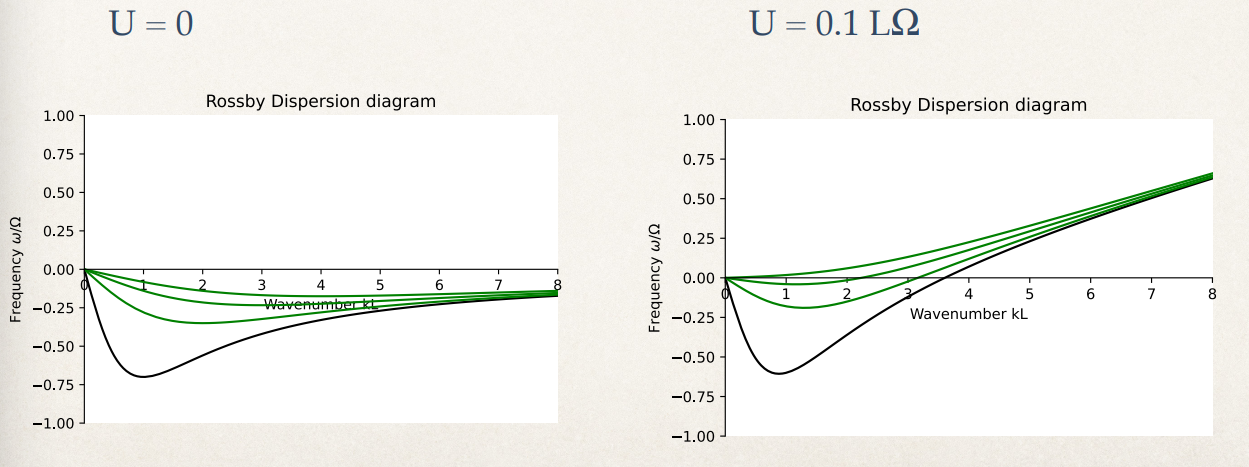
\includegraphics[width=0.5\linewidth]{upload/Screenshot 2024-11-21 162828.png}
	\caption{Rossby waves}
	\label{fig:ross waves}
\end{figure}

\section{Fundamental processes}
Different climate models incorporate all the complex physical processes occurring in the climate system using a variety of methods. The dynamic involves interactions between motions, thermodynamics, and atmospheric water content.

\subsection{Radiation}
The radiation that heats and cools the climate system can be divided into two parts: solar radiation (shortwave) and terrestrial radiation (longwave).
All gases emit and absorb radiation, and each chemical element or combination of elements has a distinct spectrum indicating at which electromagnetic wavelengths its emissions occur. In some cases, the emission may be confined to narrow portions of the electromagnetic spectrum rather than being a smoothly varying function of wavelength. This phenomenon of distinct, discrete emission spectra results from the emission of radiation as an electron moves from one orbit around an atomic nucleus to another orbit closer to the nucleus. If the atom is excited by absorbing energy, then the electron can go to a higher (outer) discrete orbit.
As electrons return to the inner orbits, emission occurs in the ultraviolet part of the spectrum, producing the emission spectra. If electrons return to intermediate orbits instead of higher orbits, the emission is in the visible part of the spectrum; for the outer orbits, the emission is in the infrared.
So far we have discussed only the emission of energy from a gas, not the absorption of energy. Suppose radiational energy enters an atomic or molecular gas and is absorbed. In that case, it can increase the atomic or molecular energy levels by the same amount of energy involved in the emission. This absorption can be just as discrete or selective as the emission. Thus, if radiation entering a gas cannot excite the atoms or molecules in any energy form, then the radiational energy will not be absorbed or emitted in the gas.\\


In the Earth's atmosphere, ozone, carbon dioxide, and water vapor are very important triatomic molecules that both emit and absorb radiation in certain parts of the electromagnetic spectrum that affect the climate system.

\begin{figure}[htp!]
	\centering
	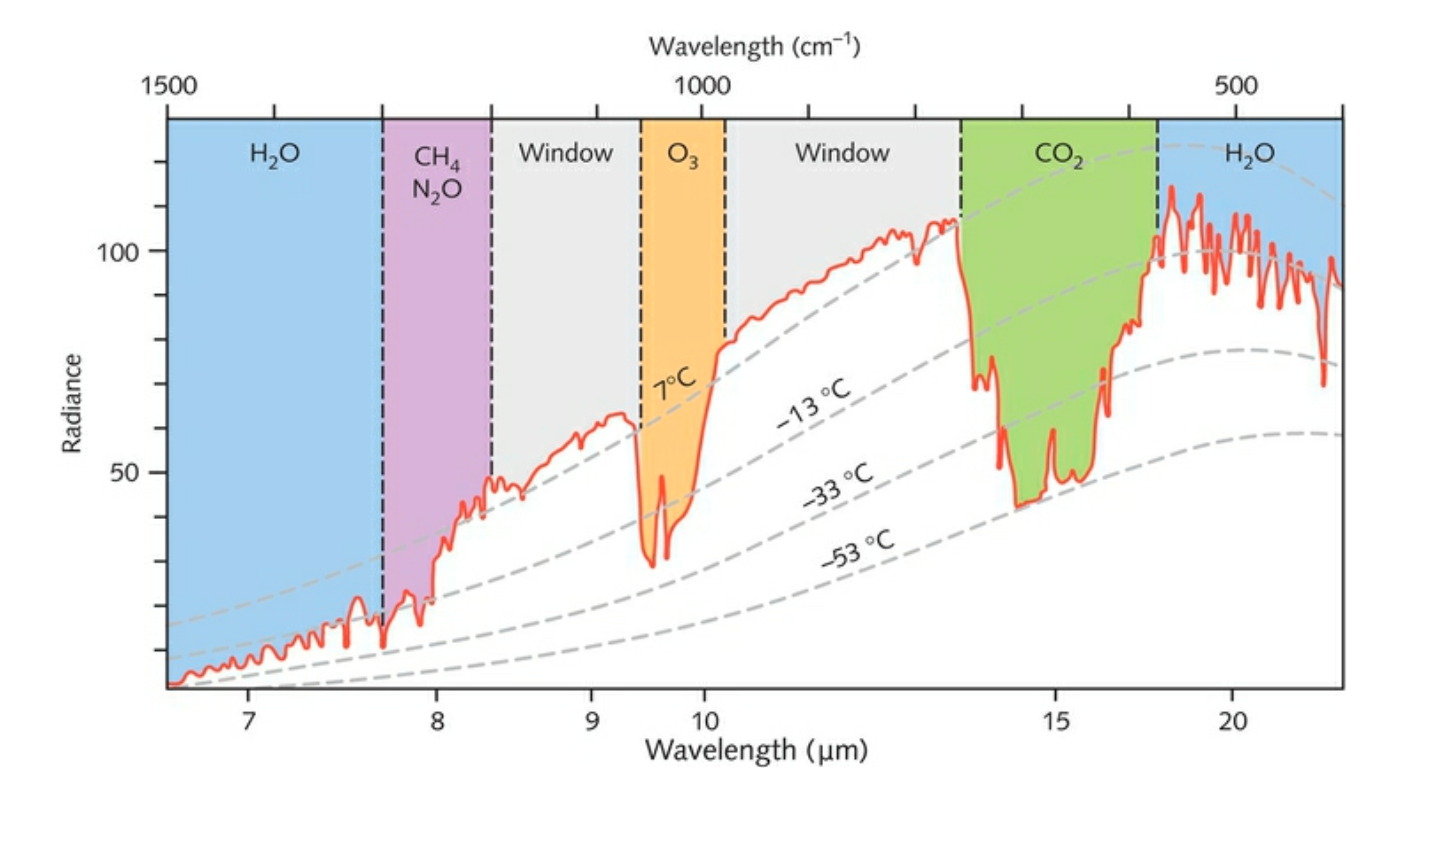
\includegraphics[width=0.5\linewidth]{upload/image10.png}
	\caption{Earth's spectrum}
	\label{fig:2.7}
\end{figure}
As we can see in figure \ref{fig:2.7} ozone is a very strong absorber in the 9-10 $\mu$m region, carbon dioxide has absorption maxima in the 2, 3, 4, and 13-17 $\mu$m regions, and water vapor has several absorption regions in the 1-8 $\mu$m range and at wavelengths greater than 13 $\mu$m.

The radiational heating and cooling computation in climate models is usually done by calculating upward and downward fluxes through unit horizontal areas, considering the vertical distributions of temperature, water vapor, and other radiative absorbing gases such as carbon dioxide and ozone.

The blackbody radiation curve was determined theoretically by Max Planck in 1900. A result of Planck's equation is the earlier displacement law of Wien, that the wavelength of maximum intensity $\frac{2897.8}{T}$ where $T$ is the temperature of the blackbody.
For the Earth, the approximate global mean surface temperature is 293 K, which yields a maximum intensity near 9.9$\mu$m whereas for the sun the surface temperature is approximately $T$ = 6110K which yields a maximum intensity at 0.474$\mu$m The overlap of the blackbody radiation curves for the Earth and for the sun's radiation reaching the Earth is not great, and consequently solar and terrestrial radiation can be separated based on wavelength.

\begin{figure}[htp!]
	\centering
	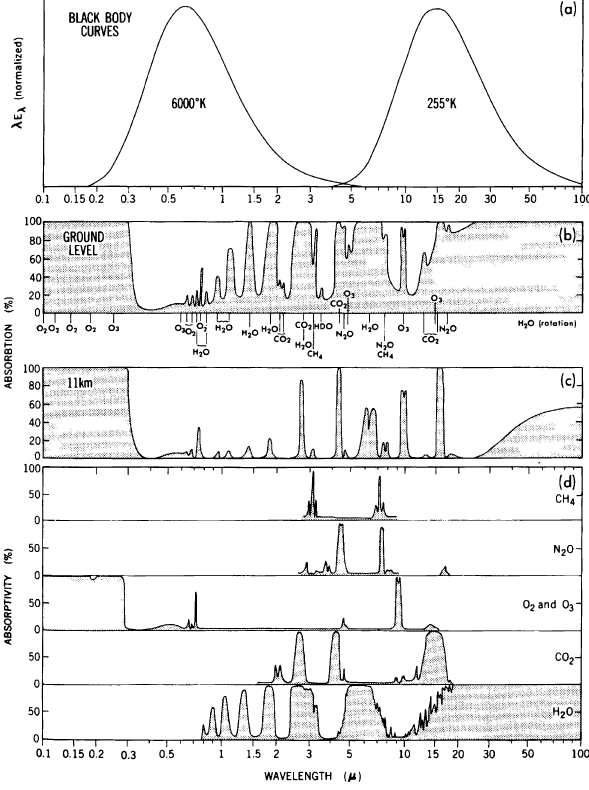
\includegraphics[width=0.4\linewidth]{upload/image11.png}
	\caption{Black body curves for the solar radiation and the terrestrial radiation for the entire atmosphere and the first 11 km of the atmosphere}

\end{figure}
Much of the fundamental physics governing radiation transfer is embodied in the following two laws:
\begin{itemize}
	\item Lambert's law, which provides a formulation for the decrease in intensity of radiation of a given wavelength as the radiation passes through a given amount of absorbing gas
	      $$\frac{d}{dz}[I]=-Ik\rho$$
	      where $k$ is the absorption coefficient (which tells us what kind of mass is preset), $\rho$ is the density of the layer, and $I$ is the radiance, defined as the energy per unit time per  unit area per unit solid angle $d\omega$

	\item Kirchhoff's law, states that there is a proportionality between radiative absorptivity and emissivity of a gas at the same temperature for any wavelength. A good absorber of radiation at some wavelength is also a good emitter of radiation at the same wavelength.

	      In particular, it is usually identified as \textit{absorptivity} the ratio of the amount of radiative energy absorbed to the total incident radiation, and \textit{emissivity} is the ratio of the emitted radiation to the maximum possible emitted radiation at the same temperature.
\end{itemize}


The \ref{fig:relat} shows the relationship between intensity from some given direction, unit solid angle $d\omega$, and the surface,
\begin{wrapfigure}{R}{0.38\textwidth}
	\begin{center}
		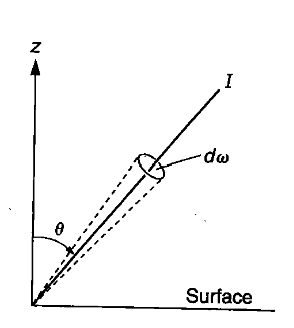
\includegraphics[width=0.22\textwidth]{upload/imageIw.png}
	\end{center}
	\caption{Relationship between intensity}
	\label{fig:relat}
\end{wrapfigure}

such that integration over $\theta$ of the hemisphere above the horizontal surface yields the flux, $F$, arriving from all angles:
\begin{equation}\label{eq 2}
	F=\int(Icos\theta )\,d\omega
\end{equation}

Dividing \ref{eq 2} by $I$ and forming integrals over optical depth on either side yield
$$\int \frac{dI}{I} = - \int k \rho \, dz$$ which becomes $$\ln \left( \frac{I}{I_0} \right) = - \int k \rho \, dz$$
upon integrating the left-hand side.
This can be written exponentially as $$I = I_0 e^{-\chi}$$

$$\chi=\int k \rho \,dz $$


where $\chi$ is the optical depth or optical path length (rate at which the radiance is degraded, if you move upward, at a certain point you get zero because you have traveled enough to absorb all the radiation)  and
$$\tau = e^{-\chi}$$
is the frictional transmission, indicating the fraction of the original radiance that get transmitted to optical depth within attenuating gas. If $\chi=1$, then $\tau=0.37$ , which means the initial intensity $I$ is decreased by a factor of $0.63$ , for normal atmospheric conditions $\chi$ in typically much less than $1$.


For a blackbody, the emission is also described by Lambert's law with a different sign
\begin{equation}\label{eq3}
	dI = B(T) k \rho \, dz
\end{equation}

Integrating \ref{eq3} over a hemisphere, the Stefan-Boltzmann law is then obtained
$$\int_0^{2\pi} B(T) \cos \theta \, d\omega = \sigma T^4$$
or $$\pi B(T) = \sigma T^4$$

The change of radiance at a point z is made up of two fluxes
$$\frac{1}{\rho} \frac{dI}{dz} = -k (I - B(T))$$ where $kI$ is the absorption and $kB(T)$ is the emission.
So the fractional absorption in a layer ($z$,$z_1$) is $$\tau(z, z_1) = \exp \left( - \int_{z_1}^z k \rho \, dz' \right)$$
\begin{figure}[htbp]
	\centering
	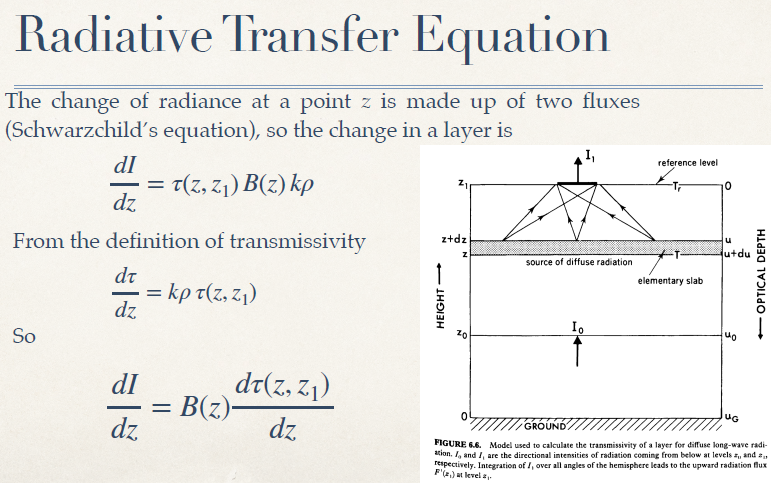
\includegraphics[width=0.35\linewidth]{upload/16image.png}\quad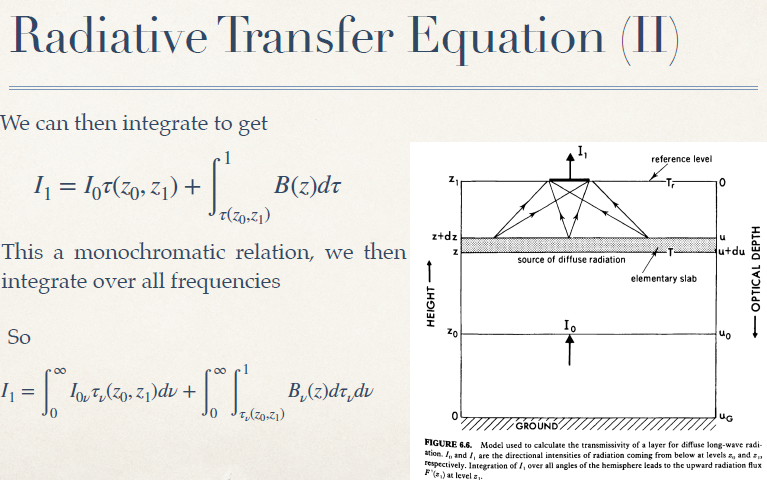
\includegraphics[width=0.35\linewidth]{uploads/17image.png}
	\caption{Non avevamo voglia di scriverli}

\end{figure}




\begin{figure}[htpb]
	\centering
	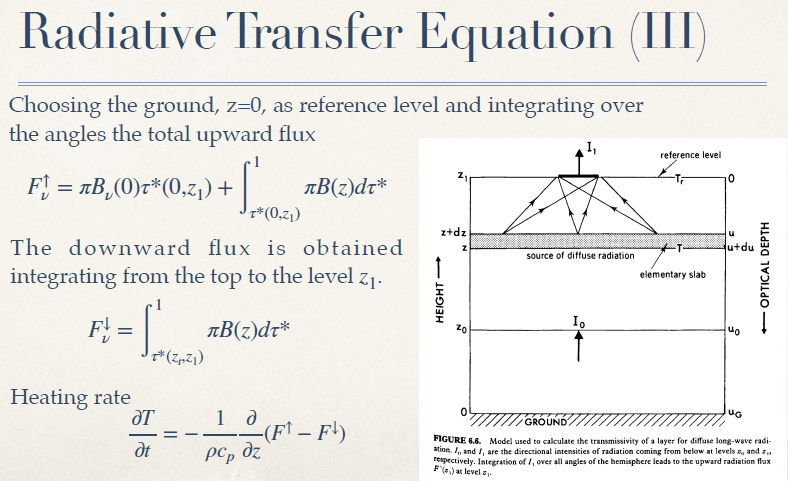
\includegraphics[width=0.5\linewidth]{upload/18image.png}
\end{figure}

\paragraph{Solar radiation} The solar radiation is a function of the zenith angle
$$\cos Z = \sin \varphi \sin \delta + \cos \varphi \cos \delta \cos H$$

where $\varphi$ is latitude, $\delta$ is solar declination, which is the angular distance of the sun north of the equator and varies from about 23.5° on June 22 to -23.5° on December 22 and H is the hour angle, which is the longitudinal distance from the point in question to the meridian of solar noon and therefore is 0 at any point experiencing solar noon.
The solar flux, $S$, entering at the top of the atmosphere is a function of $\cos Z$ and the distance from the sun to the Earth, $d$, such that
$$S = S_0 f(d) \cos Z$$
where $S_{0}$ is the so-called solar constant (the solar energy flux received at the outer atmosphere on a surface normal to the solar beam; known now not to be constant) and the factor $f(d)$ is $1.0344$ in early January and $0.9674$ in July for the present astronomical conditions.
\begin{figure}[htp!]
	\centering
	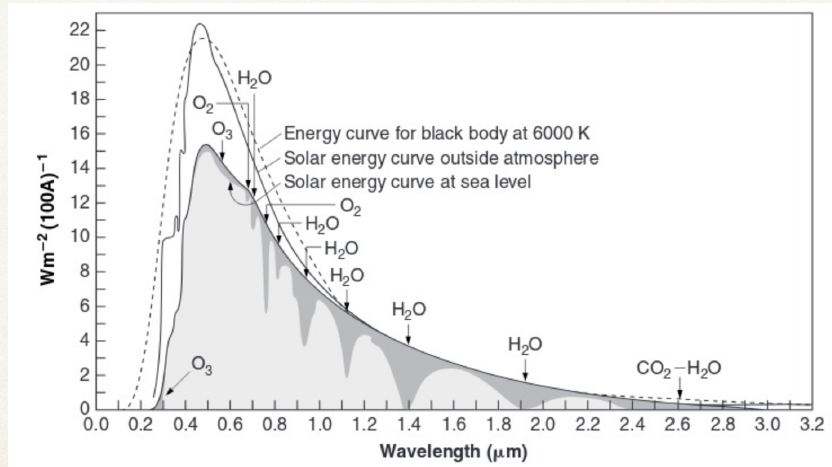
\includegraphics[width=0.5\linewidth]{upload/image12.png}
	\caption{Spectral energy distribution as a function of wavelength at the top of the atmosphere and at sea level. The figure includes absorption by various atmospheric gases}
	\label{fig1}

\end{figure}
As shown in \ref{fig1} the principal absorber in the atmosphere is the stratospheric ozone, which absorbs very effectively in the ultraviolet and in the visible. Water vapor is the primary absorber in the troposphere in the near-infrared, also with carbon dioxide are the main important absorbers for the longer wavelengths.

\begin{figure}[htp!]
	\centering
	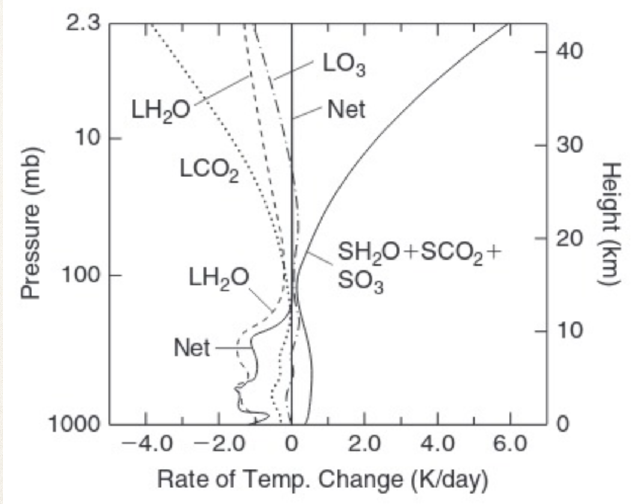
\includegraphics[width=0.4\linewidth]{upload/image13.png}
	\caption{Heating rates in the atmosphere due to the absorption of solar radiation by atmospheric gases and due to the longwave or infrared radiation}
	\label{figl}
\end{figure}
The largest contributors to the eating/cooling rates are water vapor, carbon dioxide and ozone as shown in Figure \ref{figl}.
The net heating/cooling is zero in the stratosphere because in the one-dimensional model, it is in radiative equilibrium. The troposphere shows a net radiative cooling that is compensated by the vertical transfer of sensible and latent heat from below by moist adiabatic convection. As suggested in Figure \ref{figl} water vapor is the strongest contributor to the troposphere cooling. In the stratosphere cooling due to water vapor, carbon dioxide and ozone is generally compensated by heating due to absorption of solar radiation by zone.

\subsection{Moisture}
In order to discuss precipitation and cloud physics used in climate models, let's introduce basic concepts.
\textit{Moisture} is the quantity of water vapor in the air and it can be specified in several ways, depending on which reference is used.
\begin{itemize}
	\item \textit{mixing ratio} ratio of the density of water vapor to the density of dry air $q=\frac{\rho_w}{\rho}$
	\item \textit{specific humidity} ratio concerning the density of moist air, the density of water vapor over the total density of the air: $h=\frac{\rho_w}{q_w+\rho}$
	\item \textit{relative humidity} ratio of the mixing ratio to the saturation mixing ratio $r=\frac{q}{q_s}$
\end{itemize}
The same as the continuity mass treatment, the changes in the amount of water vapor must be balanced by the moisture sources and sinks
\begin{equation}\label{eqmpis}
	\frac{dq}{dt}= \frac{1}{\rho}M + E
\end{equation}

where M is the time rate change of water vapor per unit volume due to condensation or freezing (sinks of moisture) and E is the time rate of change of water vapor content per unit mass due to evaporation from the surface and sub-grid vertical and horizontal diffusion of moisture within the atmosphere (source of moisture). The first term on the right is a sink of moisture, the second is a source of moisture.
Often \ref{eqmpis} is written in flux form by combining with the continuity equation to obtain

\begin{equation}\label{eq4}
	\frac{\partial (\rho q)}{\partial t} + \nabla \cdot (\rho q \vec{V}) + \frac{\partial (\rho q \omega)}{\partial z} = M + \rho E
\end{equation}

If \ref{eq4} is integrated over the entire volume of the atmosphere, the second and the third terms on the left drop out, so that the sources and sinks of moisture must balance to have no secular change in atmospheric moisture over the globe.
If the atmosphere is saturated with moisture, then sensible heat can be added to the atmospheric system from latent heat by the conversion of water vapor to liquid warmer or ice parcels.

The first law of thermodynamic must incorporate in the nonadiabatic term, this energy conversion process due to phase changes between liquid, solid, and gas.
If the nonadiabatic process of conversion of water vapor to liquid water is the only energy source incorporated, the first law of thermodynamics becomes
$$c_p \, dT + \frac{1}{\rho} \, dp = - L \, dqs$$
The equation of state can be written like $$e = \rho_{W} RT$$ where $e$ is the partial pressure for water vapor.
Substituting in the previous equation, the mixing ratio becomes now
\begin{equation}\label{eq2}
	q\approx 0.622 \frac{e}{p}
\end{equation}

Inserting a total differential form of the hydrostatic equation, the first law of thermodynamics becomes $$\frac{dT}{dz} = - \frac{g}{c_p} - \frac{L}{c_p} \frac{dqs}{dz}$$
taking the log and differentiating the previous equation \ref{eq2} we will obtain
$$\log q_s \approx \log 0.622 + \log e_s - \log p$$
$$\frac{1}{e_s} \frac{d e_s}{d z} = \frac{1}{q_s} \frac{d q_s}{d z} + \frac{1}{p} \frac{d p}{d z}$$
$$\frac{1}{e_s} \frac{d e_s}{d T} = \frac{1}{q_s} \frac{d q_s}{d z} - \frac{1}{p} g \rho$$

The Clausius-Clapeyron equation relates the change in saturation vapor pressure to the latent heat involved in a phase change from water vapor to liquid water or from liquid water to ice. The most convenient form of this is $$\frac{1}{e_s} \frac{d e_s}{d T} = \frac{L}{R T^2}$$
So we get $$\frac{d q_s}{d z} = \frac{L q_s}{R W T_2} \frac{d T}{d z} + \frac{g q_s}{R T}$$

\begin{equation}\label{eq.adiabatic lapse rate}
	\Gamma_m= \frac{dT}{dz} = -\frac{g}{c_p} \left( 1 + \frac{L q_s}{R T} \right) \left( 1 + \frac{L^2 q_s}{c_p R W T_2} \right)^{-1}
\end{equation}
In this way, we will obtain the moist adiabatic lapse rate $\Gamma_m$, which is less than the adiabatic lapse rate defined earlier: $$\Gamma=\frac{dT}{dz}=-\frac{k\rho g}{p}T$$



\subsection{Clouds}
They play a critical role in the radiation characteristics of the Earth's climate, but their radiative properties are not fully understood. In most climate models, the precipitation and convective aspects of the model are used to compute where clouds exist based on whether the atmosphere is near saturation and whether convection is occurring. You can use different parameters to explain that.

\subsubsection{Cumulus formation}
If a parcel of air near the Earth's surface (at an atmospheric pressure of approximately 1000 mb) starts to rise, say from strong heating, it will cool at approximately the dry adiabatic lapse rate of 9.8 Kkm-¹. When the parcel cools sufficiently the parcel is saturated, gaining a condition of instability because there is much more energy in the water vapor. The level at which this occurs is termed the lifting condensation level, LCL, and is typically at the cloud base as the picture below shows.
\begin{figure}[htpb]
	\centering
	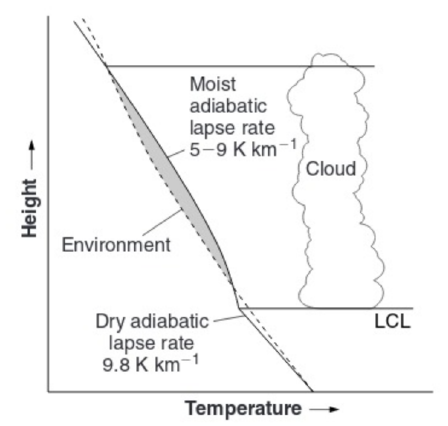
\includegraphics[width=0.4\linewidth]{upload/image14.png}

\end{figure}
If the parcel does not rise high enough to reach an LCL, then a cloud should not form. From the LCL upward, the parcel will cool less rapidly as it rises since the latent heat of condensation or fusion releases heat. This lessened rate of temperature decrease with height is the moist adiabatic lapse rate.

\begin{figure}[htpb]
	\centering
	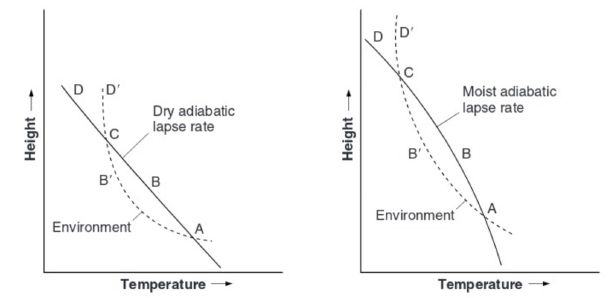
\includegraphics[width=0.5\linewidth]{upload/image15.png}
	\caption{Diagram of stable and unstable conditions concerning dry and moist lapse rates.}
	\label{fig: figure 15}
\end{figure}
As shown in figure \ref{fig: figure 15} the dotted curve represents conditions for the environmental air, and the solid curves represent conditions for the path along which a parcel will ascend from point A to B, depending on whether the dry or the moist adiabatic lapse rate is appropriate. There is a point B' highlighted on the curve for the environmental air that is colder in both cases than point B for the parcel at the same height. Since the air at B' is colder than that at B, the parcel will have positive buoyancy. Thus in principle, it will continue ascending. If on the other hand, a parcel is at C and ascends to point D, it will be colder than the surrounding environmental air at D'. Thus the parcel will have negative buoyancy, which will cause it to sink to its original position.

\subsection{Surface Processes}
Boundary fluxes for momentum and heat, we can physically represent as
$$\tau_x = \rho C_D \left| \vec{v} - \vec{v_s} \right| (u_s - u)$$
$$\tau_y = \rho C_D \left| \vec{v} - \vec{v_s} \right| (v_s - v)$$
$$H = \rho c_p C_H \left| \vec{v} - \vec{v_s} \right| (\theta_s - \theta)$$
$$LE = \rho L_C E \left| \vec{v} - \vec{v_s} \right| (q_s - q)$$

Where over land $\vec{v}$ is zero.

Above the surface boundary layer adjacent to Earth's surface exists the planetary boundary layer, where the wind turns with the height. Within this region, the balance of forces can be approximated by Coriolis, pressure gradient, and frictional forces through the following simplification
$$-f_{\nu} = - \frac{1}{\rho a \cos \varphi} \frac{\partial p}{\partial \lambda} + F_{\lambda}$$
$$f_u = - \frac{1}{\rho a} \frac{\partial p}{\partial \varphi} + F_{\varphi}$$

The frictional term can be expressed as the vertical gradient of stress, so that $$F_\lambda = \frac{1}{\rho} \frac{\partial \tau_\lambda}{\partial z}$$
and $$F_\varphi = \frac{1}{\rho} \frac{\partial \tau_\varphi}{\partial z}$$


and the stress can in turn be related to the vertical gradient of wind shear
$$\tau_\lambda = \rho K_m \frac{\partial u}{\partial z}$$
and $$\tau_\varphi = \rho K_m \frac{\partial v}{\partial z}$$

where Km is the vertical eddy or transfer coefficient for momentum. Note that if the vertical wind shear is large, as one would expect near the Earth's surface since the wind must approach zero at the surface, then the momentum transfer is also large. On the molecular scale, Km, takes on values appropriate for those space scales; however, in the atmosphere and ocean models the space scales are much larger. Many of the eddies have dimensions of the order of the spatial grid structure of the models.
If the layer is unstable there is strong vertical mixing and Km is large; if the layer is stable there is no strong coupling and Km is small. A useful measure of this stability is the Richardson number $Ri$, which is defined as
$$R_i = \frac{g}{\theta} \frac{\frac{\partial \theta}{\partial z}}{\left( \frac{\partial V}{\partial z} \right)^2}$$
where $V = \left| \vec{V} \right|$ and $\frac{\partial V}{\partial z}$ is the vertical wind shear or vertical gradient of wind velocity.

\subsection{Hydrology}
\begin{figure}[htp!]
	\centering
	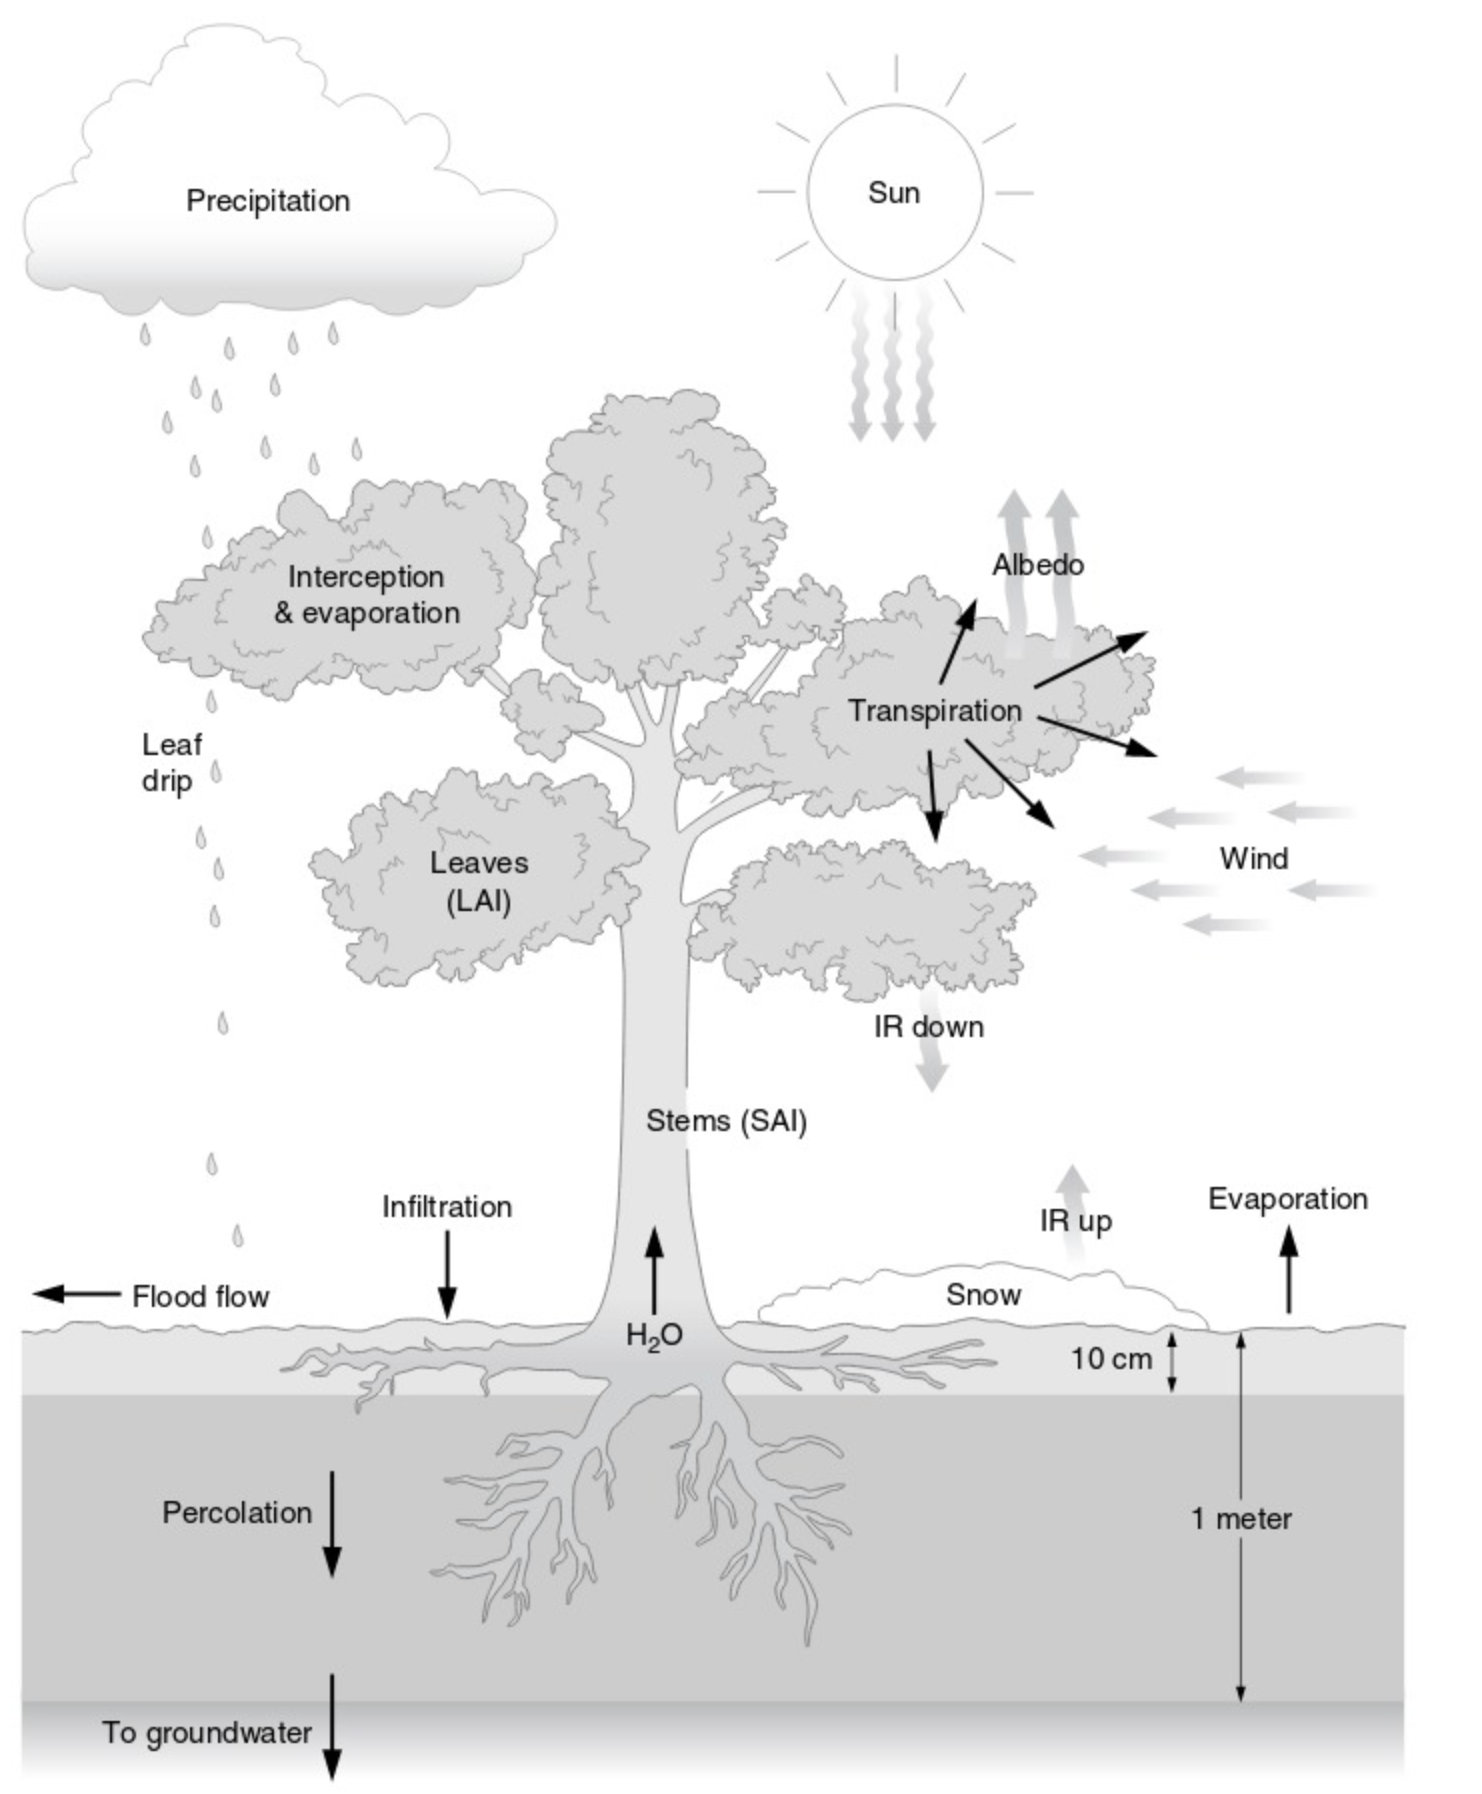
\includegraphics[width=0.5\linewidth]{upload/15image.png}
	\caption{Schematic processes and features relevant to surface hydrology and evapotraspiration}
	\label{fig: fig 2}
\end{figure}
As shown in \ref{fig: fig 2} lots of processes are involved in surface hydrology. These include radiation, sensible heat, evaporation, transpiration, momentum, and precipitation, but also H2O and CO2 fluxes. The surface moisture can contribute to surface flow in streams percolate to a deeper layer or even become groundwater, depending on the porous properties of the ground. In the root zones of plants, some of the surface moisture can be taken up by the plant roots and then relayed to the plant leaves and transpired.

Within a land area as large as a horizontal grid cell of a global model, there are generally multiple surface types, including lakes, wetlands, different vegetation types, and different soil types
Another aspect of land surface processes being improved in many climate models is the simulation of snow coverage. The snow modeling community has developed a variety of models that can be used for climate and hydrology. These models range from the simple to the complex, and several of them are specifically designed for use in general circulation models. The more complex snow models take into account melting processes, grain size, shape, liquid water content, and percolation processes.

\chapter{Numerical methods used in atmospheric models}\label{ch:chapter3}
\lastupdated{2025-02-26}{\chapterThreeNumMethOverleaf}

\begin{center}
	\textit{Major content of this chapter is taken from prof.Navarra's teaching resources, available in his website \url{https://wanderer.cmcc.it/index_GARP.html}}
\end{center}
\section{Historical introduction}
In this chapter, following a short historical introduction on the development and use of numerical methods in atmospheric models, methods available for numerical solution of the differential equations governing the atmosphere will be briefly reviewed. Then, basic elements of the finite difference method for solving these equations will be introduced. Finally, the concept of stability of finite difference equations, and methods for testing the stability of such equations, will be discussed at some length.

It is considered that Wilhelm Bjerknes (1904) was the first to point out that the future state of the atmosphere can in principle be obtained by an integration of differential equations which govern the behavior of the atmosphere, using as initial values fields describing an observed state of the atmosphere. Such an integration performed using numerical methods is called \textit{numerical weather prediction}. When, however, a numerical integration is performed starting from fictitious initial fields, it is called \textit{numerical simulation}.

A first practical attempt at a numerical weather prediction was made by Richardson. After very tedious and time-consuming computations, carried out mostly during the First World War, Richardson obtained a totally unacceptable result. Despite this, he described his method and results in a book (Richardson, 1922), and this is today one of the most famous in meteorology.

The wrong result obtained by Richardson, and his estimate that 64,000 men are necessary to advance the calculations as fast as the weather itself is advancing, left some doubt as to whether the method would be of practical use. A number of developments that followed, however, improved the situation. Courant, Friedrichs and Lewy (1928) found that space and time increments in integrations of this type have to meet a certain stability criterion. Mainly due to the work of Rossby in the late 1930’s, it became understood that even a rather simple equation, that describing the conservation of absolute vorticity following the motion of air particles, suffices for an approximate description of large-scale motions of the atmosphere. Finally, in 1945, the first electronic computer ENIAC (Electronic Numerical Integrator and Computer) was constructed. The absolute vorticity conservation equation, and this first electronic computer, were used by Charney, Fjortoft and von Neumann in the late 1940’s for the first successful numerical forecast (Charney et al., 1950).

Much faster computers, and improved understanding of computational problems, now also enable long-term integrations of the basic primitive equations. It is generally considered that integration of the primitive equations enables easier incorporation of various physical processes than the integration of modified equations, that is, integration of the divergence and vorticity equations. Thus, it is mostly the primitive equations that are used today for practical numerical forecasting by meteorological services. Charts obtained by numerical forecasting are used by synopticians in these services as the principal basis for decisions on forecasts issued for public use.

A number of research groups have been actively engaged for more than a decade in development of models for the numerical simulation of the general circulation of the atmosphere. In such simulations starting from a fictitious initial state, e.g. an isothermal and motionless atmosphere, is often considered to be an advantage for the experiments. It enables a test of the ability of the computational and physical schemes of the model to simulate an atmosphere with statistical properties similar to those of the real atmosphere, with no, or not much, prior information on these properties.

Numerical models are also very frequently developed for studies of some smaller-scale atmospheric phenomena. Foremost among these are studies of the cumulus convection problem, and simulation of processes within the planetary boundary layer. In this text, however, we shall primarily have in mind the application of numerical methods to prediction and simulation of large-scale atmospheric motions.



\section{Methods for the numerical solution of the equations of motion}
Numerical solution of the equations of motion today in most cases is performed using the \textit{grid point method}. In this method a set of points is introduced in the region of interest and dependent variables are initially defined and subsequently computed at these points. This set of points is called the grid. The words mesh or lattice are also used. It is necessary to have the grid points at fixed locations in the horizontal. This means that, according to the Eulerian system of equations, space and time coordinates are chosen as independent variables.

A number of attempts have been made to develop atmospheric models using an approach which is at least partly Lagrangian\footnote{The Eulerian approach focuses on observing how a field (like fluid flow) changes at fixed points in space over time, much like watching traffic from a fixed camera. In contrast, the Lagrangian approach tracks individual elements or particles as they move through space and time, similar to following a specific car on its journey. Essentially, Eulerian examines the "big picture" from a stationary perspective, while Lagrangian follows individual components in motion.}. Serious difficulties are encountered when a straightforward numerical integration of the Lagrangian system of equations is undertaken. However, it is possible to construct methods with some Lagrangian properties; for example, to have some or all of the compu­tation points moving with the fluid. In hydrodynamics a number of such methods have proved to be very useful, especially for some problems which are not amenable to treatment by a strictly Eulerian technique (e.g. Harlow and Amsden, 1971). However, in meteorology the per­formance of Lagrangian or semi-Lagrangian models that have so far been developed has not been quite satis­factory. A discussion of one way of constructing a Lagrangian model, and a review of earlier attempts, can be found in a paper by Mesinger (1971).

Another possible approach is to express the spatial dependence of the variables in terms of a series of ortho­gonal functions, and then substitute this into the governing equations. In this way the equations reduce to a set of ordinary differential equations, so that the coefficients of the series can be computed as functions of time. This is the \textit{spectral method} of solving the governing equations. Until relatively recently it was considered that in effi­ciency the spectral method could not be competitive with the grid point method. But the use of the fast Fourier transform has completely changed the situation and investigation of spectral methods is now the subject of intensive research.

In the following we shall consider the technique of using the grid point method, and the problems associated with it, using grid of computation points fixed in space. This is the most direct way of solving the equations of motion numerically. Furthermore, knowledge of this method is necessary for the investigation and understanding of the relative merits of other alternatives mentioned in this section.
\section{Grid point method}
With the grid point method, the most common way of solving the governing equations is to find approximate expressions for derivatives appearing in the equations. These approximate expressions are defined using only values of the dependent variables at the grid points, and at discrete time intervals. Thus, they are formed using differences of dependent variables over finite space and time intervals; for that reason this approach is called the \textit{finite difference method}. The approximations for derivatives are then used to construct a system of algebraic equations that approximates the governing partial differential equations. This algebraic system is considered valid at each of the interior grid points of the computation region. For the initial time and at space boundary points, additional constraints or equa­tions are defined that approximate the initial and bound­ary conditions as required by the physics of the problem. The set of algebraic equations obtained in this way is then solved, usually using an electronic computer, by a suitable step-wise procedure.

We shall now consider some basic elements of the finite difference method. For simplicity, we start by considering a function of one independent variable $$u=u(x)$$
The function $u$ is a solution to a differential equation that we are interested in. We want to find an approxima­tion to this solution in a bounded region R of the inde­pendent variable, having a length \textit{L}. The simplest way of introducing a set of grid points is to require that they divide the region R into an integer number of intervals of equal length $\Delta x$. This length $\Delta x$ is called the \textit{grid interval}, or \textit{grid length}. Let us denote the number of grid intervals by \textit{J}. It is convenient to locate the origin of the \textit{x} axis at the left-hand end of the region R. Thus, we are looking for approximations to $u(x)$ at discrete points $x=j\Delta x$, where \textit{j} takes integer values 0,1,2,… \textit{J}. These approximate values we shall denote by $$u_j=u_j(j\Delta x)$$
Thus, we are interested in finding \textit{J} + 1 values $u_j$

Knowledge of a discrete set of values $u_j$, even if the approximations were perfect, offers, obviously, less information than knowledge of the function $u(x)$. Let us briefly consider the situation in that respect. We shall very often find it convenient to think of the function $u(x)$ as being formed by a sum of its Fourier compo­nents, that is
$$u(x)=\frac{a_0}{2}+\displaystyle\sum_{n\geq 1}[a_n\cos\big(2\pi n\frac{x}{L}\big)+b_n\sin\big(2\pi n\frac{x}{L}\big)]$$

Now, the available \textit{J} + 1 values $u_j$ do not enable the computation of all of the coefficients $a_nb_n$; rather, they can be used to compute only \textit{J} + 1 different coefficients. A natural choice is to assume that the \textit{J} + 1 values $u_j$ define the near value $a_0$ and as many as possible of the coefficients of the Fourier components at the long wave length end of the series, that is, coefficients for \textit{n} = 1,2,3,…, \textit{J/} 2. Of these components, the one with the shortest wavelength will have $n=J/2$, with the wave length
$$\frac{L}{n}=\frac{2L}{j}=\frac{2L}{\frac{L}{\Delta x}}=2\Delta x$$
Having made that choice, we can say that with values $u_j$ at discrete points $x=j\Delta x$ it is not possible to resolve waves with wave length shorter that $2\Delta x$.
Now let us consider the differences between values $u$ that will be used to construct approximations to derivatives. These differences are called \textit{finite differences}. They can be calculated over one or more of the intervals $\Delta x$. Depending on the relation of the points from which the values are taken to the point where the derivative is required, they can be \textit{centered or uncentered}. An un-centered difference is, for example, the \textit{forward} difference

\begin{equation}\label{eq: forward difference}
	\Delta u_j=u_{j+1}-u_j
\end{equation}
more often centered (or central) differences are used, such as
\begin{equation}
	\Delta u_{j+1/2}=u_{j+1}-u_j
\end{equation}
In a centered difference the difference is between values symmetrical about the point where the difference is being calculated.

One way to construct an approximation to a differential equation is to simply replace the derivatives by appropriate \textit{finite difference quotients}. For example, for the first derivative one can use the approximation (in a forward difference scheme):
\begin{equation}\label{eq.finite diff der approx}
	\left(\frac{d u}{dx}\right)_j\rightarrow\frac{u_{j+1}-u_j}{\Delta x}
\end{equation}
The finite difference quotient here is, of course, only one of many possible approximations to the first derivative at point j.

If a finite difference quotient, or a more complex expression, is to be used as an approximation to a deri­vative, it is required, above all, that this approximation be consistent. This means that the approximation should approach the derivative when the grid interval approaches zero. The quotient \ref{eq.finite diff der approx} , obviously, has that property.

Important information is obatined when the true solution $u(j\Delta x)$ is substituted into an approximation to the derivative in place of the grid point values $u_j$, and$ u(j\Delta x)$ is expanded in a Taylor series about the central point. For the quotient \ref{eq.finite diff der approx} this procedure gives
\begin{equation}
	\frac{u_{j+1}-u_j}{\Delta x}\rightarrow\left(\frac{du}{dx}\right)_j+\frac{1}{2}\left(\frac{d^2u}{dx^2}\right)_j\Delta x+\frac{1}{6}\left(\frac{d^3u}{dx^3}\right)_j(\Delta x)^2+\dots
\end{equation}
The difference between this expression and the derivative $$\left(\frac{du}{dx}\right)_j$$ being approximated. In this case:
\begin{equation}
	\epsilon= \frac{1}{2}\left(\frac{d^2u}{dx^2}\right)\Delta x+\frac{1}{6}\left(\frac{d^3u}{dx^3}\right)_j
\end{equation}
is called the \textit{truncation error} of the approximation to the derivative. These are terms that were "truncated off" to form the approximation. The truncation error gives a measure of how accurately the difference quotient approximates the derivative for small values of $\Delta x$. The usual measure of this is the order of accuracy of an approximation. This is the lowest power of $\Delta x$ that appears in the truncation error. Thus, approximation \ref{eq.finite diff der approx}
is of the first order of accuracy. We can write
\begin{equation}
	\epsilon =o(\Delta x)
\end{equation}
For an approximation to the derivative to be consistent it must, obviously, be at least first order accurate.
\subsection{Finite difference schemes}
The algebraic equation obtained when derivatives in a differential equation are replaced by appropriate finite difference approximations is called a finite difference approximation to that differential equation, or a finite difference scheme. In this section we shall introduce the concepts of consistency, truncation error, and accuracy, for a finite difference scheme.

As an example, we shall use the linear advection equation
\begin{align}\label{eq:linear adv eq}
	\frac{\partial u}{\partial t}+d\frac{\partial u}{\partial x}=0 \notag \\
	u=u(x,t)
\end{align}
$c$ is a positive constant.
It describes advection of the variable $u$ at a constant velocity $c$ in the direction of the $x$ axis. The solution to this simple equation can, of course, also be obtained by an analytic method. It will be useful to obtain the analytic solution first, in order to investigate properties of numerical solutions by comparing them against known properties of the true solution.

It is convenient to this end to change from variables $x$, $t$ to variables $\xi$ and $t$ with the substitution $\xi=x-ct$.

Using the notation
$$u^{(x,t)}=U(\xi,t)$$
we obtain:
\begin{align}
	\frac{\partial u}{\partial t}=\frac{\partial U}{\partial\xi}\frac{\partial\xi}{\partial t}+\frac{\partial U}{\partial t}\frac{\partial t}{\partial t}=-c\frac{\partial U}{\partial\xi}+\frac{\partial U}{\partial t} \\
	\frac{\partial u}{\partial x}=\frac{\partial U}{\partial\xi}\frac{\partial\xi}{\partial x}+\frac{\partial U}{\partial t}\frac{\partial t}{\partial x}=\frac{\partial U}{\partial\xi}
\end{align}
that, substitued into \ref{eq:linear adv eq}, gives
$$\frac{\partial}{\partial t}U(\xi, t)=0$$
Thus, it is seen that U cannot be a function of $t$, but can be an arbitrary function of $\xi$. A solution of \ref{eq:linear adv eq} is, therefore,
\begin{equation}\label{eq:sol of linear adv eq}
	u=f(x-ct)
\end{equation}
where $f$ is an arbitrary function. This, we see, is the general solution of the advection equation \ref{eq:linear adv eq}, since it can satisfy an arbitrary initial condition
\begin{equation}
	u(x,0)=F(x)
\end{equation}
Thus,
\begin{equation}
	u=F(x-ct)
\end{equation}
is the solution of \ref{eq:linear adv eq} satisfying the initial conditions.
For a physical interpretation, it is often convenient to consider the solution in the $x, t$ plane. In the present case, we see that the solution takes constant values along the straight lines
$$x-ct= \text{const}$$
These lines are the \textit{characteristics} of the advection equa­tion. We can say that the solution propagates along the characteristics.\\





Let us now construct a scheme for finding an approxi­mate solution to \ref{eq:linear adv eq} using the grid point method.

We are now looking only for an approximate solution at the discrete points in the $(x,t)$ plane formed by the grid shown in the figure below. The approximate solution at a point $(j\Delta x,n\Delta t)$ is denoted by $u^n_j$.
\begin{figure}[htpb]
	\centering
	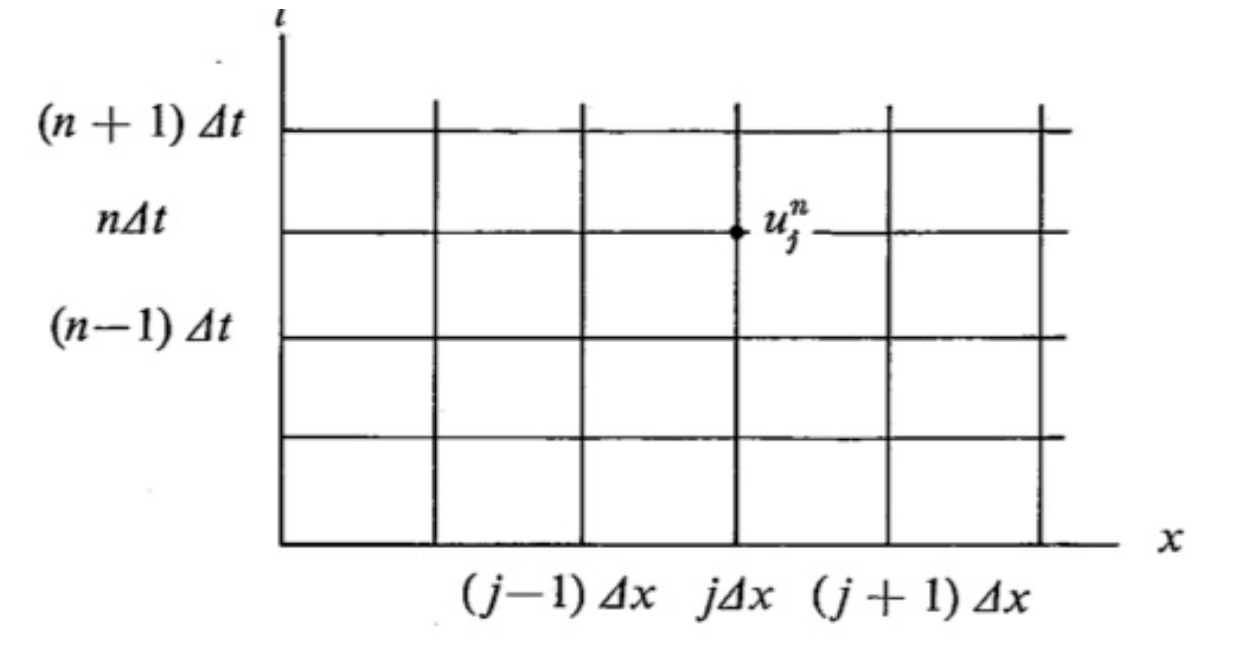
\includegraphics[width=0.35\linewidth]{upload/Screenshot 2024-12-07 163047.png}
	\caption{A finite difference grid for finding an approximate solution of \ref{eq:linear adv eq}}
	\label{fig:grid sol lin adv eq}
\end{figure}

The behaviour of the true solution, which propagates along characteristics in the $(x,t)$ plane, suggests constructing the approximate equation by replacing the time derivative by a forward difference quotient, and the space derivative by a backward difference quotient. In this way we obtain the scheme
\begin{equation}\label{eq:forward and upward scheme}
	\frac{u_j^{n+1}-u_j^n}{\Delta t}+c\frac{u_j^n-u^n_{j-1}}{\Delta x}=0
\end{equation}

This scheme could be called a forward and upstream scheme, the latter word indicating the position of the point $j-1$ relative to the advection velocity. It is, of course, only one of many possible consistent finite difference schemes for the differential equation. There are many schemes which approach the differential equation when the increments $\Delta x,\Delta t$ approach zero.

Since for small values of $\Delta x, \Delta t$ a finite difference equation approximates the corresponding differential equation, we can expect that its solution will be an approximation to the solution of that equation. We shall call solutions given by finite difference schemes numerical solutions. There are, of course, both approximate and numerical solutions obtained by other methods which will not be considered in this publication. It is most convenient to study the properties of numerical solutions when they can be compared with known solutions of the original differential equation, which we shall refer to as true solutions. The difference between the numerical and the true solution
\begin{equation}
	u_j^n-u(j\Delta x,n\Delta t)
\end{equation}
is the error of the numerical solution. For obvious reasons, we cannot often expect to know the error of the numerical solution. However, we can always find a measure of the accuracy of the scheme by substituting the true solution $u(j\Delta x, n\Delta t)$ of the equation, into the numerical scheme. Since the true solution will not satisfy the numerical equations exactly, we will have to add an additional term to keep the equation valid. Let us denote this term by $\epsilon$. For example, in the case of scheme \ref{eq:forward and upward scheme} this procedure gives
\begin{equation}\label{eq:2.4.7}
	\frac{u(j\Delta x,(n+1)\Delta t)-u(j\Delta x, n\Delta t)}{\Delta t}+c\frac{u(j\Delta x, n\Delta t)-u((j-1\Delta x, \Delta t)}{\Delta x}=\epsilon
\end{equation}
The term $\epsilon$ we shall call the truncation error of the finite difference scheme. It shows how closely the true solution satisfies the equation of the scheme, and, thus, gives a measure of the accuracy of the scheme.

We can obtain a more useful form for the expression for the truncation error by performing a Taylor series expansion of the true solution about the central space and time point. Using the original differential equation to eliminate the leading term we obtain the truncation error \ref{eq:2.4.7}:
\begin{equation}\label{eq: 2.4.8}
	\epsilon=\frac{1}{2}\frac{\partial^2u}{\partial t^2}\Delta t+\frac{1}{6}\frac{\partial^3u}{\partial t^3}(\Delta t)^2+\dots-c\left(\frac{1}{2}\frac{\partial^2u}{\partial x^2}\Delta x-\frac{1}{6}\frac{\partial^3u}{\partial t^3}(\Delta x)^2+\dots\right)
\end{equation}
As before, these are the terms that were “truncated off” to make the differential equation reduce to our finite difference scheme.

In the same way as for an approximation to the derivative, the order of accuracy of a finite difference scheme is the lowest power of $\Delta x$ and $\Delta t$ that appears in the truncation error. Thus, scheme \ref{eq:forward and upward scheme} is first order accurate. We can write
$$\epsilon=o(\Delta t)+o(\Delta x)=o(\Delta x,\Delta t)$$
It is useful to make a distinction between orders of accuracy in space and in time, especially when the lowest powers of $\Delta x$ and $\Delta t$ are not the same. As before, a necessary condition for consistency of a scheme is that it be at least of the first order of accuracy.
\subsection{Convergence}
The truncation error of a consistent scheme can be made arbitrarily small by a sufficient reduction of the increments $\Delta x$ and $\Delta t$. Unfortunately, we cannot be sure that this will also result in a reduction of the error of the numerical solution. For that reason, we return to consideration of the error
$$u_j^n-u(j\Delta x,n\Delta t)$$
Following Richtmyer and Morton (1967) we ask two questions:
\begin{itemize}
	\item What us the bahaviour of the error $u_j^n-u(j\Delta x, n\Delta t)$ when, for a fixed total time $n\Delta t$ the increments $\Delta x, \Delta t$ approach zero?
	\item What is the behaviour of the error $u_j^n-u(j\Delta x, n\Delta t)$ when, for fixed values of $\Delta x, \Delta t$, the number of time steps $n$ increases?
\end{itemize}

The answer to the first of these questions depends on the convergence of the numerical solution: if the error approaches zero as the grid is refined (as $\Delta x\Delta t\rightarrow 0$) the solution is called convergent. If a scheme gives a convergent solution for any initial conditions, then the scheme also is called convergent.

Consistency of a scheme does not guarantee convergence. We shall illustrate this by a simple example. We still consider the scheme \ref{eq:forward and upward scheme}; its truncation error \ref{eq: 2.4.8} approaches zero as the grid is refined, and, therefore, this is a consistent scheme. But consider the numerical solution, when the grid lines and characteristics are as shown in the figure below. The characteristic passing through the grid point taken as the origin in this example passes through another grid point, A, denoted by a square. Thus, the true solution at A, is equal to the initial value at the origin. However the numerical solution given by \ref{eq:forward and upward scheme} A is computed using the values at points denoted by circles. The shaded domain, including all of these points, is called \textit{the domain of dependence} of the numerical scheme. The grid point at the origin is outside that domain, and, thus, cannot affect the numerical solution at $A_0$. Therefore, the error can be arbitrarily great. If the space and time steps were reduced by the same relative amount, say to one half of their values in the figure, the domain of dependence would still remain the same, and this situation would not change. Thus, as long as the ratio of the steps $\Delta x$ and $\Delta t$ remains the same, refinement of the grid cannot bring about a reduction in the error of the numerical solution.
$$x-ct=\text{const}$$
A necessary condition for convergence of a scheme is, obviously, that the characteristic defining the true solution at a grid point is inside the domain of dependence of the numerical solution at that point. In our example, this will happen when the slope of the characteristics is greater than the slope of the dashed line bounding the domain of dependence, that is, when $$c\Delta t\leq \Delta x$$
thus, this is a necessary condition for convergence of \ref{eq:forward and upward scheme}
\begin{figure}[h]
	\centering
	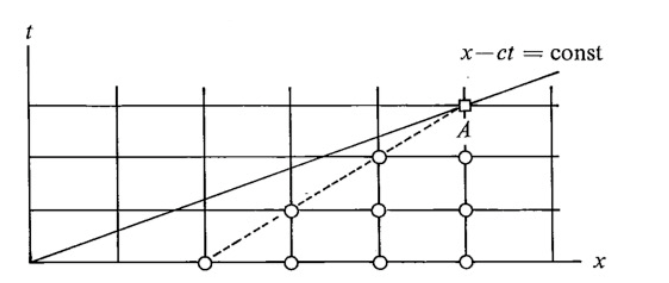
\includegraphics[width=7cm]{upload/Screenshot 2024-11-10 192132.png}
	\caption{A possible relative position of a characteristic and of a domain of dependence}
	\label{fig:grid sol}
\end{figure}
\subsection{Stability}
The answer to the second question raised at the beginning of the section Convergence "What is the behaviour of the error $u_j^n-u(j\Delta x, n\Delta t)$ when, for fixed values of $\Delta x, \Delta t$, the number of time steps $n$ increases?" depends on the stability of the numerical solution. A rigorous definition fo stability employs the concepts of functional analysis, and refers to the boundedness of the numerical solution only (e.g. Richtmyer and Morton, 1967). The difficulties in defining stability are caused by the fact that the true solution, in general, does not have to be bounded. However, when we know that the true solution is bounded, as in the equations we are interested in here, we can use a definition referring to the boundedness of the error $u_j^n-u(j\Delta x, n\Delta t)$. We said that a solution $u_j^n$ is stable if this error remains bounded as $n$ increases, for fixed values of $\Delta x, \Delta t$. As before, we say that \textbf{a finite difference scheme is stable if it gives a stable solution for any initial condition}.

Stability of a scheme is a property of great practical significance. There are consistent schemes, of a high order of accuracy, that still give solutions diverging unacceptably fast from the true solution. Thus, conditions for stability, if any, should be known. There are three methods that can be used to investigate the stability of a scheme, and we shall give an example of each of these methods. We shall do this by considering again the forward and upstream scheme \ref{eq:forward and upward scheme}.


\textcolor{Blue}{\textit{Direct method}} tests mathematically the stability of a scheme. Since we know that the true solution is bounded, it suffices to test the boundedness of the numerical solution. The scheme \ref{eq:forward and upward scheme} can be written as
\begin{equation}\label{2.6.1}
	u_j^{n+1}=(1+\mu)u_j^n+\mu u^n_{j-1}
\end{equation}
where
$$\mu=c\frac{\Delta t}{\Delta x}$$
if $1-\mu\geq 0$, which happens to be also the necessary condition for convergence, we will have:
\begin{equation}\label{2.6.2}
	|\mu_j^{n+1}|\leq(1-\mu)|u_j^n|+\mu|u^n_{j-1}|
\end{equation}
We can apply this at the point where at time level $n+1$, $|u_j^{n+1}|$ is a maximum, $Max_{(j)}|u_j^{n+1}|$. The right side of \ref{2.6.2} can only be increased by replacing $|u_j^n$ and $|u_{j-1}^n|$ by the maximum value at level $n$, $Max_{(j)}|u_j^n|$. The two terms on the right side can be added, and we obtain
$$Max_{(j)}|u_j^{n+1}|\leq Max_{(j)}|u_j^n|$$
This proves the boundedness of the numerical solution. Hence, $1-\mu\geq 0$ is seen to be a sufficient condition for stability of \ref{2.6.1}.

This direct testing of the stability is simple. Unfortunately, as might be anticipated from the argument, it is successful only for a rather limited number of schemes.\\



\textcolor{Blue}{\textit{Energy method}}. This method is of a much wider applicability, and can be used even for nonlinear equations. If we know that the true solution is bounded, we test whether
$$\displaystyle\sum_j(u_j^n)^2$$
is also bounded.
If it is, then every value \(u_j^n\) must be bounded, and the stability of the scheme has been proved. The method is called the energy method since in physical applications \(u^2\) is often proportional to some form of energy. Of course, there are examples when this is not so.
\begin{figure}[htpb]
	\centering
	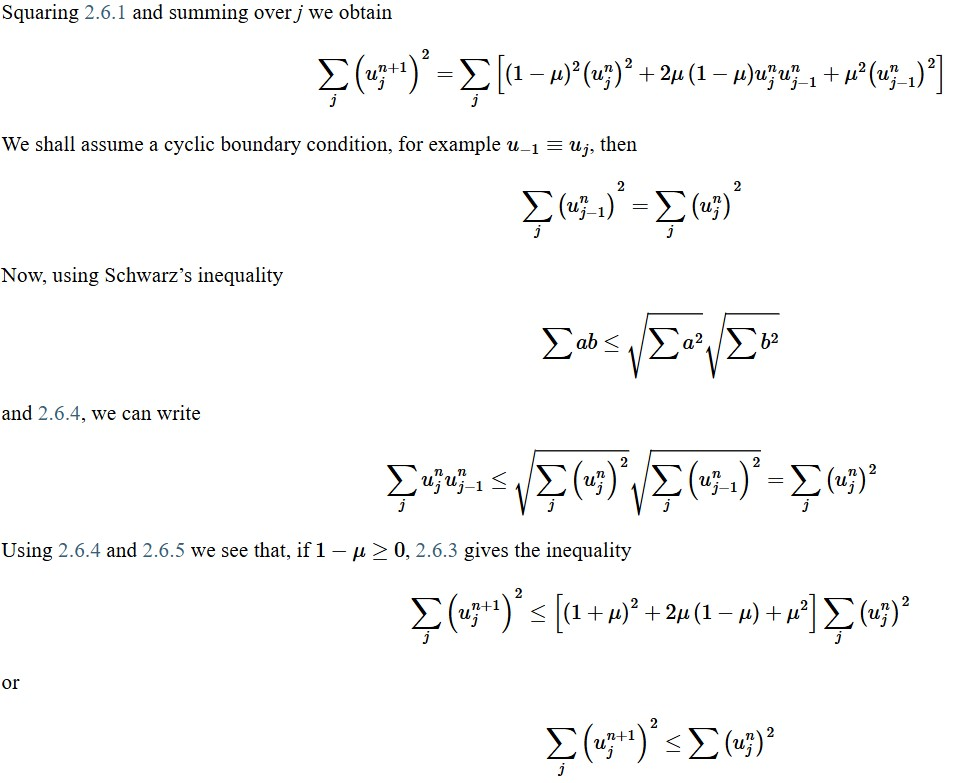
\includegraphics[width=0.75\linewidth]{upload/Immagine 2024-12-07 101350.jpg}
\end{figure}
\textit{ Von Neumann’s,} or the Fourier series method is the most frequently used method of linear equations that can be expressed in form of a Fourier series, where each harmonic component is also a solution. Thus, we can test the stability of a single harmonic solution ; stability of all admissible harmonics will then be a necessary condition for stability of the scheme.
%For an illustration of this method, it is useful first to obtain an analytic solution of the advection equation :
\begin{figure}[htpb]
	\centering
	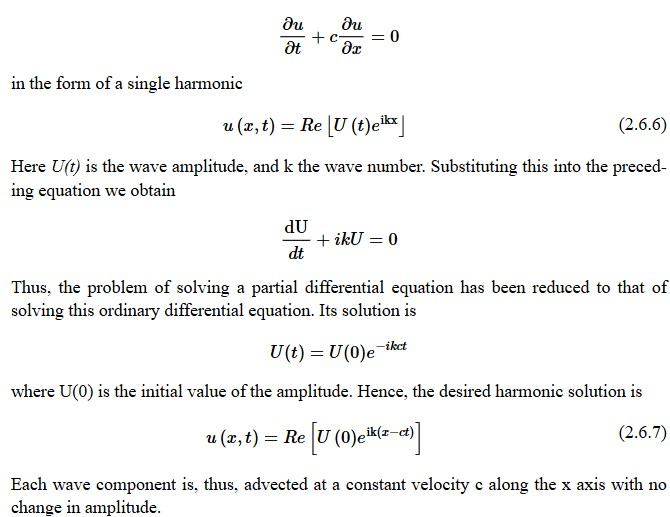
\includegraphics[width=0.70\linewidth]{upload/Immagine 2024-12-07 102403.jpg}
\end{figure}
A harmonic  solution of the finite difference advection equation.
\begin{figure}[htp!]
	\centering
	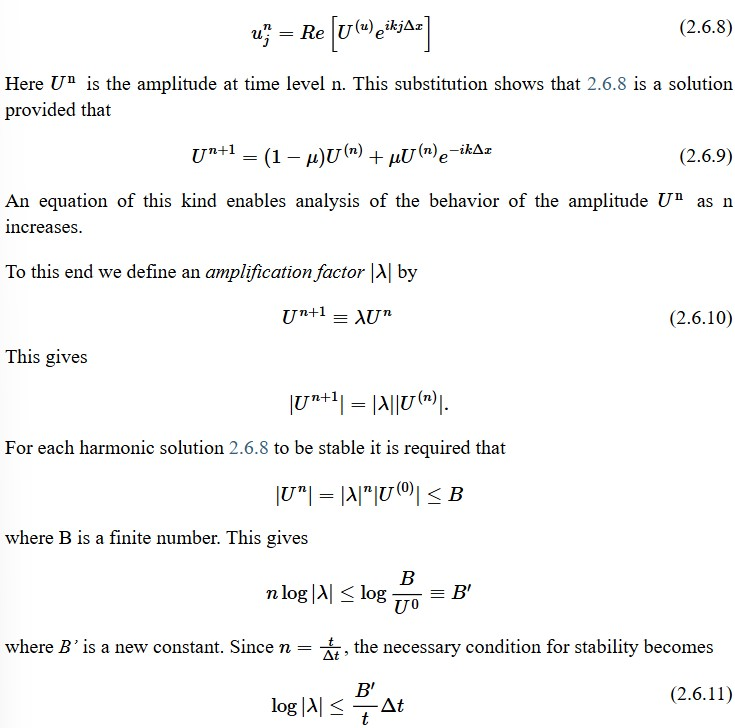
\includegraphics[width=0.65\linewidth]{upload/Immagine 2024-12-07 103148.jpg}
\end{figure}
\begin{figure}[htp!]
	\centering
	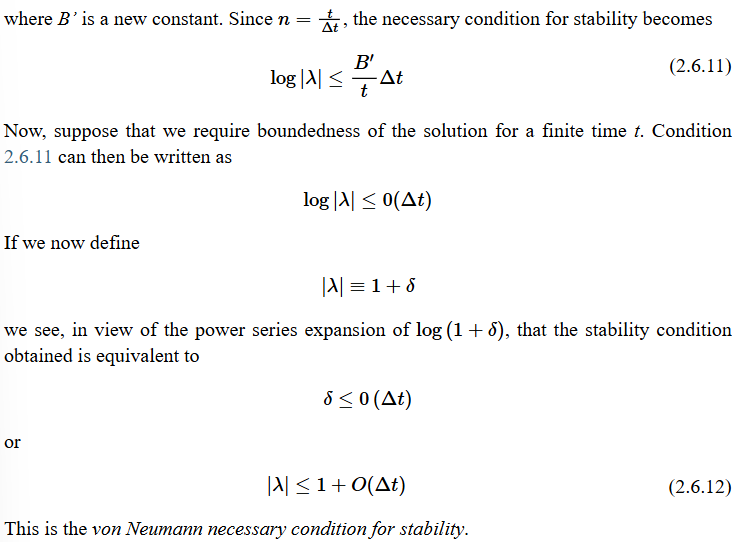
\includegraphics[width=0.65\linewidth]{upload/hhhhh.png}
\end{figure}

The Von Neumann condition permits exponential growth of the solution, but no faster. This is useful for analyzing cases where the true solution grows exponentially. However, when the true solution does not grow, as in example 2.6.7, it is common to replace the von Neumann condition with a sufficient condition, much less generous than that required by the original definition of stability : \(|\lambda|\leq1\).
\begin{figure}[htp!]
	\centering
	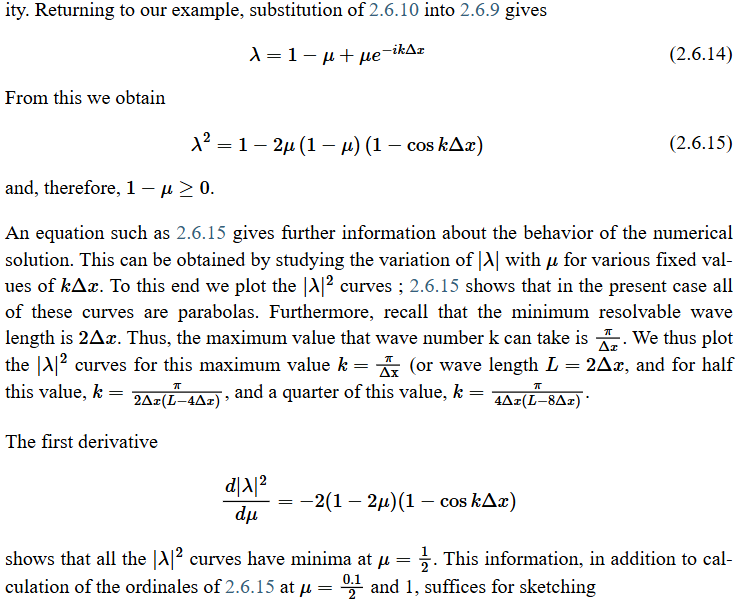
\includegraphics[width=0.65\linewidth]{upload/mi.png}
\end{figure}
\begin{figure}[htpb]
	\centering
	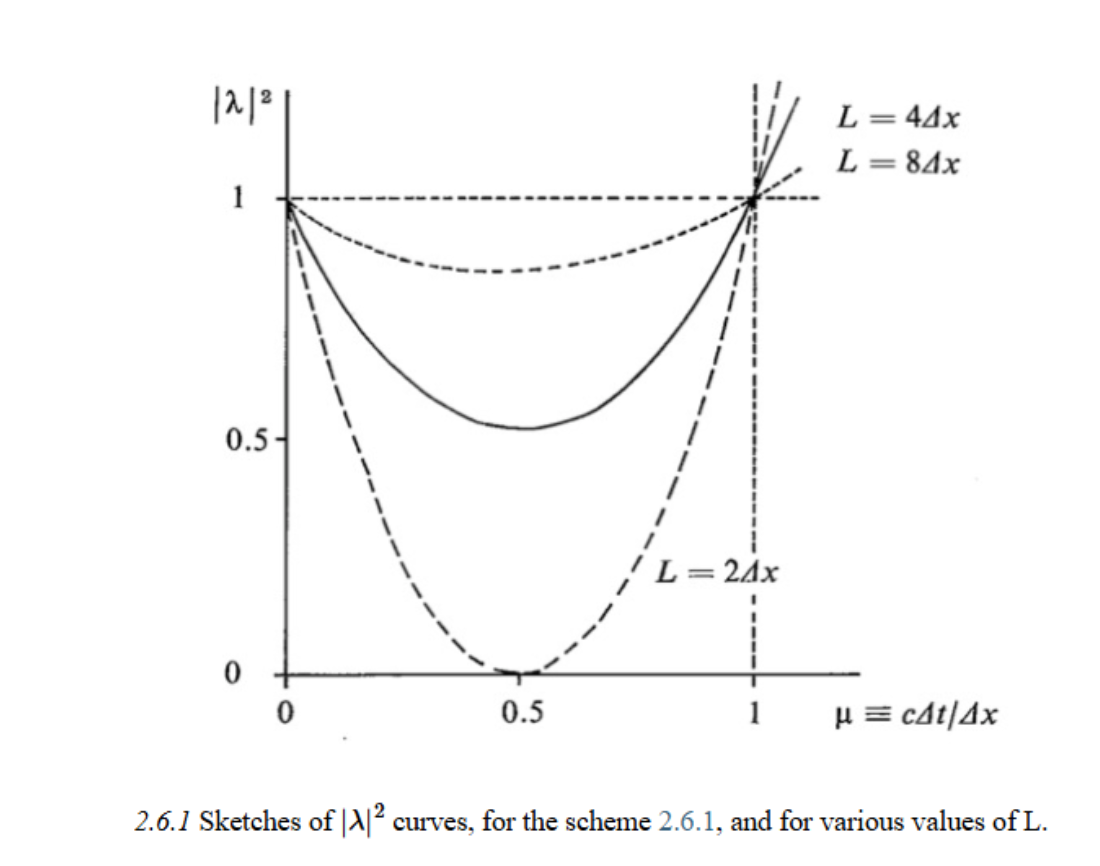
\includegraphics[width=0.45\linewidth]{upload/pp.png}
\end{figure}

The graphs of the $|\lambda|^2$ curves are shown in the picture above. In general, as the wave length $L$ increases, that is, as $k$ approaches to zero, the amplification factor approaches unity for any value of the parameter $\mu$. The figure shows that within the stable region the scheme is damping for all values $\mu\leq 1$. The damping increases as the wave length decreases. Since the true solution has a constant amplitude, this damping reveals an error due to finite differencing. We can see that this error increases as the wave length decreases. At the shortest resolvable wave length $L=2\Delta x$, the error may be very great unless $\Delta t$ extremely small. It is even possible for this wave to be completely removed after only a single time step.


The error's dependence on wavelength can be understood by considering how the finite difference grid represents harmonics of different wavelengths. The shortest resolvable wave, with only two data points per wavelength, is poorly represented. As the wavelength increases, the representation improves and approaches the continuous representation as the wavelength tends to infinity.



\section{Time differencing schemes}
In this chapter we consider ordinary differential equations with one dependent and one independent variable. Although atmospheric models are essentially always models for solving a complex set of partial differential equations, in some formulations the numerical solution of ordinary differential equations forms an important part of the computational procedure. For instance in spectral models the governing partial differential equations reduce to a set of ordinary differential equations for the expansion coefficients as dependent variables. A set of ordinary differential equations will also be obtained if a Lagrangian method is used, in which the computational points move with the fluid. But, most of all, schemes for solving ordinary differential equations are of interest here since they are often used without modification to construct approximations to the time derivative terms in the governing partial differential equations. Knowledge of the properties of schemes for solving ordinary differential equations will then be used in investigating the properties of more complex schemes for solving the partial differential equations.

With that in mind, we shall here first define some of the schemes that will be interesting to analyze. Then we shall investigate the behavior of numerical solutions obtained when these schemes are used for two specific ordinary differential equations: the oscillation (or frequency) equation, and the friction equation. These equations will serve as prototypes for later extension of the results to advection, gravity-inertia wave, and diffusion processes within the atmospheric primitive equations.

Schemes used for the time derivative terms within the primitive equations are relatively simple, usually of the second and sometimes even only of the first order of accuracy. There are several reasons for this. First, it is a general experience that schemes constructed so as to have a high order of accuracy are mostly not very successful when solving partial differential equations. This is in contrast to the experience with ordinary differential equations, where very accurate schemes, such as the Runge-Kutta method, are extremely rewarding. There is a basic reason for this difference. With an ordinary differential equation, the equation and a single initial condition is all that is required for an exact solution. Thus, the error of the numerical solution is entirely due to the inadequacy of the scheme. With a partial differential equation, the error of the numerical solution is brought about both by the inadequacy of the scheme and by insufficient information about the initial conditions, since they are known only at discrete space points. Thus, an increase in the accuracy of the scheme improves only one of these two components, and the results are not too impressive.

Another reason for not requiring a scheme of high accuracy for approximations to the time derivative terms is that, in order to meet a stability requirement of the type discussed in the preceding sections, it is usually necessary to choose a time step significantly smaller than that required for adequate accuracy. With the time step usually chosen, other errors, for example in the space differencing, are much greater than those due to the time differencing. Thus, computational effort is better spent in reducing these other errors, and not in increasing the accuracy of the time differencing. This, of course, does not mean that it is not necessary to consider carefully the properties of various possible time differencing schemes. Accuracy, is only one important consideration in choosing a scheme.

To define some schemes, we consider the equation
\begin{equation}\label{eq.3.1.3}
	\frac{dU}{dt}= f(U,t) \,\, U=U(t)
\end{equation}
We divide the time axis into segments of equal length $\Delta t$. We shall denote by
$U^{(n)}$ the approximate value of U at time $n\Delta t$. We assume that we know at least the first of the values $U^{(n)}$, $U^{(n-1)}$, $\dots$ and we want to construct a scheme for computation of an approximate value $U^{(n+1)}$. These are many possibilities.
\subsubsection{Two-level schemes}
These are schemes that relate values of the dependent variable at two time levels: $n$ and $n + 1$. Only a two level scheme can be used to advance an integration over the first time step, when just a single initial condition is available. With such a scheme we want to approximate the exact formula
\begin{equation}\label{eq. 3.1.4}
	U^{(n+1)}=U^{(n)}+\int_{n\Delta t}^{(n+1)\Delta t}f(U,t)dt
\end{equation}
Schemes that don't use an iterative procedure:
\paragraph{Euler (forward) scheme}
This is the scheme
\begin{equation}\label{3.1.5}
	U^{n+1}=U^{(n)}+\Delta t\cdot f^{(n)}
\end{equation}
where
$$f^{(n)}=f\left(U^{(n)},n\Delta t\right)$$
The truncation error of this scheme is $o(\Delta t)$. Thus, this is a first order accurate scheme. For the integrand in \ref{eq. 3.1.4} we have here taken a constant value equal to that at the lower boundary of the time interval. Thus, this is an uncentered scheme.
\paragraph{Backward scheme}
We can also take a constant value of $f$ equal to that at the upper boundary of the time interval. We then obtain
\begin{equation}\label{3.1.6}
	U^{n+1}=U^{(n)}+\Delta t f^{(n+1)}
\end{equation}

If, as here, a value of $f$ depending on $U^{(n+1)}$ appears in the difference equation, the scheme is called implicit. For an ordinary differential equation, it may be simple to solve such a difference equation for the desired value $U^{(n+1)}$. But, for partial differential equations, this will require solving a set of simultaneous equations, with one equation for each of the grid points of the computation region. If a value of $f$ depending on $U^{(n+1)}$ does not appear in the difference equation the scheme is called explicit. The truncation error of this scheme is also is $o(\Delta t)$.
\paragraph{Trapezoidal scheme}
If we approximate $f$ in \ref{eq. 3.1.4} by an average of the values at the beginning and the end of the time interval, we obtain the trapezoidal scheme:
\begin{equation}\label{3.1.7}
	U^{(n+1)}=U^{(n)}+\frac{1}{2}\Delta t\left(f^{(n)}+f^{(n+1)}\right)
\end{equation}
This is also an implicit scheme. Its truncation error, however, is $o(\Delta t^2)$. To increase the accuracy or for other reasons we can also construct iterative schemes. Two level schemes that we will now define are constructed in the same way except an iterative procedure is used to make them explicit.
\paragraph{Matsuno (or Euler-backward) scheme}
With this scheme a step is made first using the Euler scheme; the value of U obtained for time level $n+1$ is then used for an approximation to $f^{n+1}$, and this approximate value $f^{(n+1)}$ is used to make a backward step. Thus,
\begin{align}\label{3.1.8}
	U^{*(n+1)}=U^{(n)}+\Delta tf^{(n)} \\
	U^{n+1}=U^{(n)}+\Delta  tf^{*(n+1)}\notag
\end{align}
where
$$f^{*(n+1)}=f\left(U^{*(n+1)}, (n+1)\Delta t\right)$$
this is an explicit scheme, of the first order of accuracy.
\paragraph{Heun scheme}
An approximation of the trapezoidal scheme. Thus,
\begin{align}
	U^{*(n+1)}=U^{(n)}+\Delta t f^{(n)} \\
	U^{(n+1)}=U^{(n)}+\frac{1}{2}\Delta t \left(f^{(n)}+f^{*(n+1}\right) \notag
\end{align}
Thus, this is also an explicit scheme. It is of the second order of accuracy.
\subsubsection{Three level schemes}
Except at the first step, one can store the value $U^{(n-1)}$, and construct schemes taking advantage of this additional information. These are three level schemes. They may approximate the formula
\begin{equation}\label{3.1.10}
	U^{(n+1)}=U^{(n-1)}+\int_{(n-1)\Delta t}^{(n+1)\Delta t}f(U,t)dt
\end{equation}
or, they can use the additional value $U^{(n-1)}$ to make a better approximation to $f$ in \ref{eq. 3.1.4}.
\paragraph{Leapfrog scheme}
The simplest way of making a centered evaluation of the integral in \ref{3.1.10} is to take for $f$ a constant value equal to that at the middle of the interval $2\Delta t$. This gives the leapfrog scheme
\begin{equation}\label{3.1.11}
	U^{(n+1)}=U^{(n-1)}+2\Delta t\cdot f^{(n)}
\end{equation}
Its truncation error is $o(\Delta t^2)$. This is probably the scheme most widely used at present in atmospheric models. It has also been called the "mid-point rule", or "step-over" scheme.
\paragraph{Adams-Bashforth scheme}
The scheme that is usually called the Adams-Bashforth scheme in the atmospheric sciences is, in fact, a simplified version of the original Adams-Bashforth scheme, which is of the fourth order of accuracy. The simplified version is obtained when
in \ref{eq. 3.1.4} is approximated by a value obtained at the centre of the interval $\Delta t$ by a linear extrapolation using values $f^{(n-1)}$ and $f^{(n)}$. This gives
\begin{equation}\label{3.1.12}
	U^{(n+1)}=U^{(n)}+\Delta t\left(\frac{3}{2}f^{(n)}-\frac{1}{2}f^{(n-1)}\right)
\end{equation}
This also is a second order accurate scheme.
There are many other possibilities. For examples, one can approximate the integral \ref{3.1.10} using Simpson's rule, that is, by fitting a parabola to the values $f^{(n-1)}$, $f^{(n)}$ and $f^{(n+1)}$.
The implicit scheme obtained in this way is called the Milne-Simpson scheme. To illustrate the wealth of possible alternatives we note that in a paper by Young (1968) properties of 13 different schemes have been studied. Furthermore, when we are solving a more complicated partial differential equation, or a system of such equations, time (or space-time) differencing schemes can be constructed which are more complex than those which can be defined using the simple equation \ref{eq.3.1.3}. Such schemes are widely used in atmospheric models, and some of them will be described in later chapters of this publication.


\subsection{Properties of schemes applied to particular equations}
\paragraph{The advective equation} $$\frac{\partial u}{\partial t}+c\frac{\partial u}{\partial x}=0$$
has a wave solution $u(x,t)=Re[U(t)e^{ikx}]$ provided that
$$\frac{dU}{dt}+ikc=0$$
this ordinary differential equation reduces to \ref{3.2.1} if we substitute $\omega=-kc$.
The general solution of \ref{3.2.1} is
$$U(t)=U(0)e^{i\omega t}$$
or, for discrete values $t=n\Delta t$:
\begin{equation}
	U(n\Delta t)=U(0)e^{in\omega\Delta t}
\end{equation}
Thus, considering the solution in a complex plane, its argument rotates by $\omega\Delta t$ in each time step and $\Delta t$ there is no change in amplitude.

The properties of various schemes when applied to \ref{3.2.1} are conveniently analyzed using the von Neumann method. This method, as we have seen, involves defining a variable $\lambda$ by
\begin{equation}\label{3.2.3}
	U^{(n+1)}=\lambda U^{(n)}
\end{equation}
with
$$\lambda=|\lambda|e^{i\theta}$$
so
\begin{equation}\label{3.2.5}
	U^{(n)}=|\lambda|U^{(0)}e^{in\theta}
\end{equation}
with $\theta$ representing the change in argument (or phase change) of the numerical solution in each time step. Since we know that the amplitude of the true solution does not change, we shall require $|\lambda|\leq 1$ for stability.
\begin{figure}[h]
	\centering
	\includegraphics[width=0.50\linewidth]{upload/Screenshot 2024-11-11 225800.png}
	\caption{stability scheme}
	\label{fig:stab scheme}
\end{figure}
It will also be instructive to compare the phase change of the numerical solution per time step, $\theta$, with that of the true solution, $\omega\Delta t$. The ratio of these changes, $\frac{\theta}{\omega\Delta t}$, is the relative phase change of the numerical solution.
\begin{figure}[h]
	\centering
	\includegraphics[width=0.50\linewidth]{upload/Screenshot 2024-11-11 230012.png}
	\caption{phase change}
	\label{fig:phase change}
\end{figure}
For accuracy, therefore, it is desirable to have both the amplification factor and the relative phase speed close to unity. Exceptions to this are so-called “computational modes”, which, as we shall see later, can appear as false solutions superposed on the physical solution. These are solutions that do not approach the true solution as the space and time steps approach zero. If such solutions exist they will each have their own value of the amplification factor. Since they are not an approximation to the true solution, it is desirable to have their amplitudes as small as possible, that is, to have their amplification factors less than unity.\\


Stability will require, where B is a constant
\begin{equation}
	|U^{(n)}|=|\lambda|^n|U^{(0)}|<B
\end{equation}
or
\begin{equation}
	n\log|\lambda|<\log\frac{B}{|U^{(0)}|}
\end{equation}
$$\log|\lambda|<\log\frac{B\Delta t}{t|U^{(0)}|}\propto \frac{B'}{t}\Delta t$$
we want however that it is valid for finite times
$$\log|\lambda|\leq o(\Delta t)$$
This means that if $\lambda=\+\delta$ the deviation must be such that $\delta\leq o(\Delta t)$ so the condition for stability is:
\begin{equation}
	|\lambda|\leq 1+o(\Delta t)
\end{equation}
this condition will allow for exponential growth, but not faster.
\paragraph{Generale formula}
The three non-iterative two level schemes can be describes by a single finite difference equation:
\begin{equation}\label{3.2.6}
	U^{(n+1)}=U^{(n)}+\Delta t\left(\alpha f^n+\beta f^{(n+1)}\right)
\end{equation}
with a consistency requirement
$$\alpha+\beta=1$$
Notice:
\begin{itemize}
	\item $\alpha=1$, $\beta =1$ for the Euler scheme
	\item $\alpha=0$, $\beta=1$ for the backward scheme
	\item $\alpha=1/2$, $\beta=1/2$ for the trapezoidal scheme
\end{itemize}
\paragraph{Oscillation equation}
For applications in atmospheric models it is of particular interest to consider the case where $$f=i\omega U$$
Model problem:
\begin{equation}\label{3.2.1}
	\frac{dU}{dt}=i\omega U
\end{equation}
$$U^{(n)}\rightarrow U(n\Delta t)$$
The equation \ref{3.2.1} is known as the oscillation equation or frequency equation. Allowing U to be complex, \ref{3.2.1} can be thought of a representing a system of two equations. The parameter $\omega$ is real, and called the frequency.
Applying \ref{3.2.3} to the oscillation equation gives
\begin{equation}
	U^{(n+1)}=U^{(n)}+i\omega\Delta t\left(\alpha U^n+\beta U^{(n+1)}\right)
\end{equation}
In order to evaluate $\lambda$ we must solve this equation for $U^{(n+1)}$. Denoting $p=\omega\Delta t$:
\begin{equation}\label{3.2.9}
	U^{(n+1)}=\frac{1+i\alpha p}{1-i\beta p}U^{(n)}
\end{equation}
Therefore
\begin{equation}\label{3.2.10}
	\lambda=\frac{1+\alpha p}{1-i\beta p}
\end{equation}
\paragraph{Euler} $\alpha=1 \, \beta=0 \, \lambda=1+ip$
so $$|\lambda|=(1+p^2)^{1/2}$$
Te Euler scheme is always unstable, however for very small time steps $\Delta t$ $p$ is so small that
$$|\lambda|\approx 1+\frac{1}{2}p^2$$
The less restrictive von Neumann criterion is satisfied. However, experience shows that an indiscriminate use of the Euler scheme for solution of the atmospheric equations leads to amplification at a quite unacceptable rate.
\paragraph{Backward} $\alpha=0 \, \beta=1 \, \lambda=\frac{1}{1+p^2}1+ip$
so $$|\lambda|=(1+p^2)^{-1/2}$$
Te backward scheme is always stable (no matter what $\Delta t$), however is also dumping, meaning it's reducing the amplitude of the solution. The amount of damping increases as the frequency $\omega$ increases. This is often considered to be a desirable property of a scheme. For instance, we can think of a system in which a number of frequencies are present at the same time; for example, solving a system of equations of the type \ref{3.2.1}. This situation is similar to that existing in the real atmosphere. It would appear to be necessary to maintain the amplitudes of motions of different frequencies in the correct ratio. However, in numerical integrations, high frequency motions are often excited to unrealistically large amplitudes through errors in the initial data. It may then be desirable to reduce the amplitudes of high frequency motions by a selective damping in the time differencing scheme. In other words, a scheme with frequency dependent damping properties can be used to filter out undesirable high frequency motions.
\paragraph{Trapezoidal} $\alpha=1/2 \quad \beta=1/2 \quad \lambda=\frac{1}{1+1/4p^2}\left(1-1/4p^2+ip\right)$
$$|\lambda|=1$$
The trapezoidal scheme is, thus, always neutral. The amplitude of the numerical solution remains constant, just as does that of the true solution. It is useful to note that both the implicit schemes considered here were stable no matter how large a value of $\Delta t$ was chosen.
\paragraph{Matsuno}
The iterative two level schemes can also be described by a single equation in the same way as \ref{3.2.6}. Thus, we write
\begin{align}\label{3.2.18}
	U^{(n+1)*}=U^{(n)}+\Delta tf^{(n)}\notag \\
	U^{(n+1)}=U^{(n)}+\Delta t\left(\alpha f^{(n)}+\beta f^{*(n+1)}\right)
\end{align}
that applied to the oscillation equation gives:
\begin{align}
	U^{(n+1)*}=U^{(n)}+i\omega\Delta tU^{(n)} \notag \\
	U^{(n+1)}=U^{(n)}+i\omega\Delta tU^{*(n+1)}
\end{align}
eliminating the intermediate values $U^{(n+1)*}$:
$$U^{(n+1)}=\left(1-\beta p^2+ip\right)U^{(n)}$$
thus,
\begin{equation}\label{3.2.20}
	\lambda=1-\beta p^2+ip
\end{equation}
Substituting the appropriate values of $\beta$ for the Matsuno scheme, we obtain
\begin{equation}\label{3.2.21}
	\lambda=1-p^2+ip
\end{equation}
and the stability condition (we need to evaluate $|\lambda|$):
\begin{equation}\label{3.2.23}
	|\lambda|=\left(1-p^2+p^4\right)^{1/2}
\end{equation}
the Matsuno scheme is stable if $|p|<1$, so the time step must be $$\Delta t\leq\frac{1}{|\omega|}$$
This scheme is conditionally stable: the higher the frequency, the more restrictive is the stability condition. When differenciating \ref{3.2.23} we find that the amplification factor of the Matsuno scheme has a minimum for $p=1/\sqrt{2}$. Therefore, as pointed out by Matsuno (1966a) when dealing with a system with a number of frequencies we can choose a time step so as to have $0\leq p\leq 1/\sqrt{2}$ for all the frequencies present, and then, in the same way as backward implicit scheme, this scheme will reduce the relative amplitudes of high frequencies. This technique has recently become very popular for initialization of atmospheric models, where it is used to damp the spurious high frequency noise generated by the assimilation of the observed data. As shown by Matsuno (1966b) higher order accuracy schemes with similar filtering characteristics can be constructed.
\begin{figure}[h]
	\centering
	\includegraphics[width=0.50\linewidth]{upload/Screenshot 2024-11-12 101958.png}
	\caption{The amplification factor as a function of $p=\omega\Delta t$, for the five two level schemes and for the true solution}
	\label{fig:3.2.1}
\end{figure}
Figure \ref{fig:3.2.1} summarizes the results obtained for the five schemes considered so far. For all of these schemes the amplification factors were found to be even functions of $p$, so the amplification factor curves are shown only for $p\geq 1$.
\paragraph{Leap-Frog scheme (Three level schemes)}
The more accurate leap-frog scheme is more delicate.
\begin{equation}\label{3.2.33}
	U^{(n+1)}=(U^{(n-1)}+2i\omega\Delta tU^{(n)}
\end{equation}
A problem with all three or more level schemes including this is that they require more than one initial condition to start the computation. From a physical standpoint a single initial condition $U^{(0)}$ should have been sufficient. However, in addition to the physical initial condition, three level schemes require a computational initial condition $U^{(1)}$. This value cannot be calculated by a three level scheme, and, therefore, it will usually have to be obtained using one of the two level schemes. According to \ref{3.2.3} we also have
\begin{equation}\label{3.2.34}
	U^{(n)}=\lambda U^{(n-1)}\,\,\, U^{(n+1)}=\lambda^2U^{(n-1)}
\end{equation}
substitued in \ref{3.2.33} we have
$$\lambda^2-2ip\lambda-1=0$$ that has solutions:
\begin{align*}
	\lambda_1=\sqrt{1+p^2}+ip \\
	\lambda_2=-\sqrt{1-p^2}+ip
\end{align*}
Thus, there are two solutions of the form $U^{(n+1)}=\lambda U^{(n)}$. This necessarily follows from the fact that we are considering a three level scheme; substitution of \ref{3.2.34} into the difference equation given by these schemes will always give a second degree equation for $\lambda$. In general, an m level scheme will give $m — 1$ solutions of the form $U^{(n+1)}=\lambda U^{(n)}$. A solution of this type corresponding to a single value of $\lambda$ is called a mode.

Consider now the two values that have been obtained for $\lambda$. If a solution of the form $U^{(n+1)}=\lambda U^{(n)}$ is to represent an approximation to the true solution, then we must have $\lambda\rightarrow 1$ as $\Delta t\rightarrow0$. For the values $\lambda_1, \lambda_2$, as $p=\omega\Delta t\rightarrow0$ we do have $\lambda_1\rightarrow1$, however at the same time $\lambda_2\rightarrow-1$. Solutions like that associated with $\lambda_1$ are usually called \textit{physical modes} because we are always solving equations describing physical processes. Solutions like that associated with $\lambda_2$ are not approximations to the true solution, and are called \textit{computational modes}.
\begin{itemize}
	\item Case $|p|<1$: then $|\lambda|=1$ stable
	\item Case $|p|=1$: then $|\lambda|=1$ equal
	\item Case $|p|>1$: then $|\lambda|=|p\pm\sqrt{p^2-1}|$ unstable
\end{itemize}
\subsubsection{Stability for dissipation equation}
For the dissipation equation
\begin{equation}\label{3.3.6}
	\frac{dU}{dt}=-kU \text{,} \,\, U=U(t)\text{,} \,\, k>0
\end{equation}
Again it is easy to justify our interest in this equation. For example, if we define $U=u+iv$, it describes the effect of friction proportional to the velocity vector, as is often assumed for motions near the ground. As another example, note that when seeking a solution of the heat transfer, or Fick’s diffusion equation in the form od a single harmonic component.
The general solution of \ref{3.3.6} is
\begin{equation}
	U(t)=U(0)e^{-kt}
\end{equation}
Thus, both the real and the imaginary part decrease exponentially with time.
The properties of schemes applied to \ref{3.3.6} will again be analyzed using the von Neumann method. As in the previous section, we consider first the non-iterative two level scheme \ref{3.2.6}. Applied to the diffusion equation, it gives:
\begin{equation}\label{3.3.8}
	U^{(n+1)}=U^{(n)}-k\Delta t\left(\alpha U^{(n)}+\beta U^{(n+1)}\right)
\end{equation}
writing $K=k\Delta t$ we have
\begin{equation}\label{3.3.10}
	U^{(n+1)}=\frac{1-\alpha K}{1+\beta K}U^{(n)}
\end{equation}
and
\begin{equation}
	\lambda=\frac{1-\alpha K}{1+\beta K}
\end{equation}
For the two level schemes we have:
\begin{itemize}
	\item Euler ($\alpha=1, \beta=0$): $\lambda=|1-K|\rightarrow0<K\leq2$ stable
	\item Backward ($\alpha=0, \beta=1$): $\lambda=\frac{1}{1+K}\rightarrow K>0$ stable
	\item Trapezoidal ($\alpha=1/2, \beta=1/2$): $\lambda=\frac{1-1/2K}{1+1/2K}\rightarrow K>0$ stable
\end{itemize}
while for the leap-frog scheme:
$$\lambda^2+2K\lambda-1=0$$
giving the solutions
\begin{align}
	\lambda_1=-K+\sqrt{1+K^2} \\
	\lambda_2=-K-\sqrt{1+K^2}\notag
\end{align}
As $k\rightarrow0$, $\lambda_1\rightarrow1$, while $\lambda_2\rightarrow-1$ thus, the solution associated with $\lambda_1$ again represents the physical mode, and that associated with $\lambda_2$ the computational mode. For  $K>0$, that is for the normal case of a forward integration in time,  this  result  always  in  a  computational  mode $\lambda_2$  that  is always  unstable. It changes sign from time step to time step, and its magnitude increases. As before, we cannot hope to eliminate the computational mode completely. Because  we  can’t  eliminate  completely  the computational   mode   the   leapfrog   cannot   be   used   for   the dissipation equation.
The  same  analysis  applied  to  the  friction  equation  will  give  a different  result.  The  Euler  scheme  is  stable  and  the  leapfrog scheme is instead is always unstable.
\subsection{A combination of schemes}
A natural question to ask at this point is what can we do if, for example, the equation contains both the oscillation and the dissipation term, that is
\begin{equation}\label{3.4.1}
	\frac{dU}{dt}=i\omega U-kU
\end{equation}
Here we might like to use the leapfrog scheme because of the oscillation term $i\omega U$, but we know that it cannot be used for the dissipative term $-kU$. In this and similar situations we can use different schemes for the different terms; for example, we might use the leapfrog scheme for the oscillation term and the forward scheme for the dissipative term. We then obtain:
\begin{equation}
	U^{(n+1)}=U^{(n-1)}+2\Delta t\left(i\omega U^{(n)}-kU^{(n-1)}\right)
\end{equation}
\section{The Advection Equation}
We now consider differential equations with one dependent and two or three independent variables, that is, partial differential equations. More specifically, we shall consider various simplified forms of the advection equation, describing advection of a dependent variable. This is considered in practice to be the most important part of the atmospheric governing equations.

We have already discussed the one-dimensional linear advection equation to some extent in the introductory chapter. We shall organize the analysis here so as first to continue considering problems associated with the simplest one-dimensional linear form of the advection equation, and then to proceed to problems introduced by more complex forms of the advection equation.
Consider the equation
\begin{equation}\label{4.1.1}
	\frac{\partial u}{\partial t}+c\frac{\partial u}{\partial x}=0
\end{equation}
here $u=u(x,f)$ is a function of two independent variables: the independent variable $x$ will represent a space variable, and, thus, \ref{4.1.1} will be called the one-dimensional linear advection equation. As seen earlier, its general solution is
$$u=f(x-ct)$$ where $f$ is an arbitrary function.
One of the finite difference schemes for \ref{4.1.1} is the forward and upstream scheme. If the space derivative (i.e. discretizing only "$x$") is approximated by a centered finite difference quotient using values at the two nearest points, we obtain for the time derivative:
\begin{equation}\label{4.1.3}
	\frac{\partial u_j}{\partial t}=-c\frac{u_{j+1}-u_{j-1}}{2\Delta x}
\end{equation}
The subscript here, as before, denotes the distance from the origin in space increments; that is, $x=j\Delta x$. A number of schemes for the numerical solution of \ref{4.1.1} can now be constructed because we can approximate the time derivative in \ref{4.1.3} by one of the methods studied in the preceding chapter. For example, when the time derivative is approximated using the leapfrog scheme, we obtain
\begin{equation}\label{4.1.4}
	\frac{u^{n+1}_j-u^{n-1}_j}{2\Delta t}=-c\frac{u_{j+1}^n-u_{j-1}^n}{2\Delta x}
\end{equation}
as one of many possible consistent schemes for the numerical solution of \ref{4.1.1}.

A possible solution of \ref{4.1.1} will be of the form
\begin{equation}\label{4.1.5}
	u_j=\text{Re}\left[U(t)e^{ikj\Delta x}\right]
\end{equation}
going back to the oscillation equation:
\begin{equation}\label{4.1.6}
	\frac{dU}{dt}=i\left(-\frac{c}{\Delta t}\sin k\Delta x\right)U
\end{equation}
denoting
$$p=-c\frac{\Delta t}{\Delta x}\sin k\Delta x$$
Now, if we approximate \ref{4.1.6} using one of the time differencing schemes, the same finite difference equation is obtained as when we apply that scheme to \ref{4.1.3} and then substitute the wave solution \ref{4.1.5}. Hence, properties of finite difference schemes derived from \ref{4.1.3} can be inferred from the results of Section Time differencing schemes, where the frequency to is given by $p=\omega\Delta t$.
As an example, if \ref{4.1.6} is approximated using the leap-frog scheme, we obtain:
\begin{equation}\label{4.1.8}
	U^{(n+1)}=U^{(n-1)}+2\left(-c\frac{\Delta t}{\Delta x}\sin k\Delta x\right)U^{(n)}
\end{equation}
with
\begin{equation}\label{4.1.9}
	p=-c\frac{\Delta t}{\Delta x}\sin k\Delta x
\end{equation}
We obtain the same finite difference equation \ref{4.1.8} by first applying the leapfrog scheme to \ref{4.1.3} giving \ref{4.1.4} and then substituting \ref{4.1.5} into \ref{4.1.4}. Thus, properties of \ref{4.1.4} can be inferred from the known properties of the leapfrog scheme applied to the oscillation equation.

Let us look at some of conclusions obtained in this way. For stability of the leapfrog scheme it was required that the condition $|p|\leq 1$ occuring. Thus, we have to satisfy
\begin{equation}
	\left|c\frac{\Delta t}{\Delta x}\sin k\Delta x\right|\leq 1
\end{equation}
for any admissible $k$. Since $|\sin k\Delta x|$ does reach the maximum value of unity in the admissible range of $k$, we obtain the stability condition
\begin{equation}\label{4.1.10}
	|c|\frac{\Delta t}{\Delta x}\leq 1
\end{equation}
This critetion (already mentioned) shows that stability cannot simply be anchieved by reduction of the time and space increments. Rather, it is necessary to reduce the ratio of these increments $\frac{\Delta x}{\Delta t}$ to obtain stability. This condition was first found by Courant, Friedrichs and Lewy (1928) and therefore, is usually referred to as the Courant-Friedrichs-Lewy, or CFL. stability criterion.

It is instructive to note that the maximum value of $|p|$, that is, the minimum stability, is associated with the wave with $k\Delta x=\frac{\pi}{2}$. This is the component with wave length $4\Delta x$, twice the shortest resolvable wave length $2\Delta x$.


Let us use now another scheme to approximate the time derivative in \ref{4.1.3}: the Matsuno scheme. First the approximate values $u_j^{(n+1)*}$ using the forward scheme, that is,
\begin{equation}\label{4.1.16}
	\frac{u_j^{(n+1)*}-u_j^n}{\Delta t}+c\frac{u^n_{j+1}-u^n_{j-1}}{2\Delta x}=0
\end{equation}
then, these approximate values are used in the backward scheme, that is,
\begin{equation}\label{4.1.17}
	\frac{u_j^{(n+1)}-u_j^n}{\Delta t}+c\frac{u_{j+1}^{(n+1)*}-u_{j-1}^{(n+1)*}}{2\Delta x}=0
\end{equation}
eliminating the intermediate step, i.e. the approximate values $u^{(n+1)*}$ , from this equation, by substituting values given by \ref{4.1.16}, with the subscript $j$ replaced by $j+1$ and then by $j-1$.
\begin{align*}
	\frac{u_{j+1}^{(n+1)*}-u_{j+1}^n}{\Delta t}+c\frac{u_{j+2}^{n}-u_{j}^{n}}{2\Delta x}=0 \\
	\frac{u_{j-1}^{(n+1)*}-u_{j-1}^n}{\Delta t}+c\frac{u_j^{n}-u_{j-2}^{n}}{2\Delta x}=0
\end{align*}
CFL criterion.
In this way we obtain:
\begin{equation}\label{4.1.18}
	\frac{u_j^{(n+1)}-u_j^n}{\Delta t}=-c\frac{u_{j+1}^{n}-u_{j-1}^{n}}{2\Delta x}+c^2\frac{u^n_{j+1}-2u^n_j+u^n_{j-2}}{2\Delta x^2}
\end{equation}
Without the last term, this represents the finite difference equation obtained when the forward scheme is used for the time derivative in \ref{4.1.3}. The third term approaches zero as $\Delta x,\Delta t\rightarrow 0$, and \ref{4.1.18} is therefore also a consistent scheme for the advection equation. On the other hand, for a fixed $\Delta t$ this term approaches $c^2\Delta t\left(\frac{\partial^2u}{\partial x^2}\right)$ as $\Delta x\rightarrow0$. It is therefore of the same form as a finite difference approximation to a Fick’s diffusion term, and it has a damping effect. This damping effect, however, is dependent on the wave length. As the third term is calculated over an interval of $4\Delta x$, the maximum damping occurs for a wave with wave length of $4\Delta x$. There is no damping of the shortest resolvable wave with wave length $2\Delta x$. Even if a damping effect were desirable when solving the advection equation, we would not want this particular dependence on wave length. Thus, the Matsuno scheme does not appear suitable for solving the advection equation.

It is convenient to include here one more example of the use of the energy method for testing stability. In addition to being applicable also to nonlinear equations, it can be used to study the effect of boundary conditions on stability. We will use the energy method here to test the stability of a group of schemes that can be used for solving \ref{4.1.3}.
The last term can be decomposed as
\begin{equation}
	\frac{u_{j+1}^n-2U_j^n+u_{j-2}^n}{2\Delta x^2}=\left(\frac{u^n_{j+2}-u^n_j}{2\Delta x}\right)-\left(\frac{u_j^n-u^n_{j-2}}{2\Delta x}\right)\frac{1}{2\Delta x}\approx \frac{\partial^2u}{\partial x^2}
\end{equation}
\begin{figure}[h]
	\centering
	\includegraphics[width=0.5\linewidth]{upload/Screenshot 2024-11-12 151817.png}
	\caption{steps}
	\label{fig:step}
\end{figure}
The scheme is adding a dissipative term.
\subsubsection{Non linear advection}
Consider now the non-linear advection equation
\begin{equation}\label{4.6.5}
	\frac{\partial u}{\partial t}=-u\frac{\partial u}{\partial x}
\end{equation}
consider the effect of the non linear term on a single wave $u=\sin kx$, a function $u(x)$ which can be represented by values at grid points. When performed on finite differences it cannot resolve wave length shorter than $2\Delta x$, or wave numbers greater than $k_{max}=\pi/\Delta x$,  $k<k_{max}$.
For the wave the non-linear term will look like:
\begin{equation}
	u\frac{\partial u}{\partial x}=k\sin kx\cos kx=\frac{1}{2}k\sin 2kx
\end{equation}
If $k$ is in the range $\frac{1}{2}k_{max}<k\leq k_{max}$ the result of the multiplication will be beyond the capability of the grid to represent. It cannot, therefore, be properly reproduced in a finite difference calculation.
To gain some insight into what happens in such a situation, consider a wave for which $k>K_{max}$. For example, let $L_t=\frac{4\Delta x}{3}$. A wave of that wave length is shown by the full line in 4.6.2. Knowing only the values at grid points we will not be able to distinguish this wave from the one shown by the dashed line. Thus, with the convention adopted earlier which assumes that the longest waves are present, we will make an error. This is called \textit{aliasing error}.
\begin{figure}[h]
	\centering
	\includegraphics[width=0.5\linewidth]{upload/Screenshot 2024-11-12 161236.png}
	\caption{A wave of wave length $\frac{4\Delta x}{3}$, misrepresented by the finite difference grid as a wave of wave length $4\Delta x$.}
	\label{fig:4.6.2}
\end{figure}
The waves with wave number $k_u>k_{max}$ will be interpreted as longer waves according to $k^*=2k_{max}-k_u$.
In a real numerical solution, higher wave numbers will be continuously be created by the non linear interactions and so the amplitude of wave numbers close to $k_{max}$ will continue to increase.\\
[0.4cm]

Now consider the consequences of aliasing errors in a numerical integration. An atmospheric variable, as a function of space co-ordinates, can be thought of as consisting of a series of harmonic components. It is useful to consider the “energy” of these components, that is, their contribution to the mean square value of the variable considered as a function of wave number.

This is the \textit{spectrum} of the “energy”. For example, if the variables are velocity components, this function is the kinetic \textit{energy spectrum}. This spectrum describes the relative importance of features of different scales in the field of the variable. Now, experience shows that the spectrum of atmospheric variables does not change much with time. On synoptic maps we do not have situations where small scale features are dominant on one day, and absent on the next. Accordingly, spectra of atmospheric variables also do not change much in their general shape. The energy of a particular component can, of course, change, but the characteristic shape of the spectrum as a whole is fairly constant. For example, a zonal spectrum of the eastward velocity component in middle latitudes typically has a maximum for wave numbers 4 to 7, that is, 4 to 7 wave lengths along a latitude circle, with the energy tapering off rather rapidly as the wave number increases beyond about 10. Thus, there is very little energy in wave numbers of the order of the maximum wave numbers that can be resolved by finite difference grids used in atmospheric models.

In a finite difference integration, in addition to these relatively small physical changes, the shape of a spectrum is subject to changes due to aliasing errors. If we have a spectrum of the shape just described, and consider the representation of various combinations $k_1+k_2$ that are greater than $k_{max}$, we see that most of the energy of such combinations will belong to components with wave numbers not much greater than $k_{max}$ . Thus, due to aliasing errors a spurious energy inflow is expected at wave numbers that are not much less than $k_{max}$, and, in time, the energy of these components can be expected to grow beyond physically acceptable limits. Experience shows that, if no precautionary measures are taken, this can indeed happen, and even cause a catastrophic end to the integration. The phenomenon is due to the nonlinear terms of the equations, and, therefore, is called the \textit{nonlinear instability}. Nonlinear instability was first encountered by Norman Phillips (1956) in his famous work that laid the foundation for the numerical modeling of the atmospheric general circulation. Starting from an atmosphere at rest, he integrated the vorticity equation for a simulated time of the order of 30 days. The calculation then came to an end due to an explosive increase in the total energy of the system, associated with an appearance of elongated shapes in the vorticity field. Phillips initially believed that the breakdown was due to excessive truncation errors, and he later repeated the experiment using space and time steps both reduced to about half of their previous values. This must have greatly reduced the truncation errors, but the catastrophic increase in total energy still happened at about the same time.

In a later paper Phillips (1959) gave the interpretation of nonlinear instability similar to what has been presented here, but for the nondivergentvorticity equation. For a test of this explanation Phillips again repeated his experiment, but after every two hours of simulated time he performed a harmonic analysis of the vorticity fields, and eliminated all components with $k>\frac{1}{2}k_{max}$. If there are no components with $k>\frac{1}{2}k_{max}$ the advection term cannot produce waves with $k>k_{max}$. We expect that it will be some time before the amplitudes of the eliminated waves are built up again to an appreciable extent. This filtering procedure eliminated the appearance of the spurious increase in energy, thereby confirming this explanation of the instability.
\section{Energy and numerical methods}\label{sec:en and numerical methods}
\begin{center}
	\textit{References for the following section can be found in the book at chapter 4.2: Finite differencing in two dimensions}
\end{center}

Some issues with nonlinear instability:
\begin{itemize}
	\item The nonlinear instability shows the issues with controlling errors that make the amplitude grow indefinitely
	\item On the other end, this issues shows that there are conservation property of the basic equations that must be reflected in the numerical scheme.
	\item This remark led to the development or the requirement that numerical scheme must be devised that have the same conservation properties of the original equation
	\item To illustrate this point we will use the simplified homogeneous flow system that we have introduced previously.
\end{itemize}
The selection of appropriate spatial finite difference formulations to use in the horizontal and vertical directions varies widely depending on which properties are being modeled or are considered important. Most climate models are not intended primarily for predicting the exact location of daily weather events with great accuracy but are directed more toward the simulation of the long-term mean and variance states of the climate system. Since the models frequently run for long periods of time, the numerical schemes used should approximately maintain many of the integral constraints that are in the original differential equations, such as conservation of mass, energy and momentum. Many climate models have employed horizontal finite difference methods that maintain these features.

Consider an incompressible fluid with a variable height, and assume that the horizontal velocity components, $u$ and $v$ are independent of height, and that the vertical velocity $w$ equals 0 at the bottom of the fluid. The set of momentum equations for a homogeneous flow are the following:
$$h=0$$
\begin{align}\label{eq.momentum}
	\frac{\partial u}{\partial t}=-u\frac{\partial u}{\partial x}-v\frac{\partial u}{\partial y}+fv-g\frac{\partial\eta}{\partial x}       \\
	\frac{\partial v}{\partial t}=-u\frac{\partial v}{\partial x}-v\frac{\partial v}{\partial y}-fu-g\frac{\partial\eta}{\partial y}\notag \\
	\frac{\partial \eta}{\partial t}=-\frac{\partial}{\partial x}u(\eta+H_0)-\frac{\partial }{\partial y}v(\eta+H_0)\notag
\end{align}
Considering the total height $H=H_0+\eta$ and multiplying the first two equations by $H$ we obtain:
\begin{align*}
	H \frac{\partial u}{\partial t}=-uH\frac{\partial u}{\partial x}-vH\frac{\partial u}{\partial y}+fHv-gH\frac{\partial\eta}{\partial x} \,\,\, \text{(1)} \\
	H\frac{\partial v}{\partial t}=-uH\frac{\partial v}{\partial x}-vH\frac{\partial v}{\partial y}-fHu-gH\frac{\partial\eta}{\partial y}\,\,\, \text{(2)}   \\
	\frac{\partial H}{\partial t}=-\frac{\partial}{\partial x}uH-\frac{\partial }{\partial y}vH \,\,\, \text{(3)}
\end{align*}
Using the relations:
\begin{equation}
	H\frac{\partial u}{\partial t}=\frac{\partial}{\partial t}(uH)-u\frac{\partial H}{\partial t}=-\frac{\partial}{\partial x}(uuH)+u\frac{\partial}{\partial x}(uH)-\frac{\partial}{\partial x}(uvH)+u\frac{\partial}{\partial x}(vH)
\end{equation}
We can rewrite the equations of motion as:
\begin{align}
	\frac{\partial uH}{\partial t}=-\frac{\partial uuH}{\partial x}-\frac{\partial uvH}{\partial y}+fHv-g\frac{\partial\eta}{\partial x}        \\
	\frac{\partial vH}{\partial t}=-\frac{\partial uvH}{\partial x}-\frac{\partial vvH}{\partial y}-fHu-gH\frac{\partial\eta}{\partial y}\notag \\
	\frac{\partial H}{\partial t}=-\frac{\partial}{\partial x}uH-\frac{\partial }{\partial y}vH\notag
\end{align}
In this form the mass equation makes mass conservation immediately visible, let us now consider energy.
Kinetic energy is defined as:
$$KE=\frac{1}{2}H(u^2+v^2)$$
and the potential energy:
$$PE=\frac{1}{2}gH^2$$
now, by multiplying eq.(1) by $Hu$ and (3) by $u^2/2$ and adding, then eq. (2) by $Hv$ and (3) by $v^2/2$ and adding, using the product derivative rule as before, we can get:
\begin{align}
	\frac{\partial}{\partial t}\left(H\frac{1}{2}u^2\right)+\frac{\partial}{\partial x}\left(Hu\frac{1}{2}u^2\right)+\frac{\partial}{\partial y}\left(Hv\frac{1}{2}u^2\right)-fHvu+gHu\frac{\partial H}{\partial x} \\
	\frac{\partial}{\partial t}\left(H\frac{1}{2}v^2\right)+\frac{\partial}{\partial x}\left(Hu\frac{1}{2}v^2\right)+\frac{\partial}{\partial y}\left(Hv\frac{1}{2}v^2\right)-fHvu+gHv\frac{\partial H}{\partial x} \\
\end{align}
multiplying the continuity equation (3) by $gH$ and rearranging we get:
\begin{equation}
	\frac{\partial}{\partial t}\left(g\frac{1}{2}H^2\right)+\frac{\partial}{\partial x}\left(gH^2u\right)+\frac{\partial}{\partial y}\left(gH^2v\right)-gH\left[u\frac{\partial H}{\partial x}+v\frac{\partial H}{\partial y}\right]=0\\
\end{equation}
The total energy is defined as:
$$TE=KE+PE=\frac{1}{2}H(u^2+v^2)+\frac{1}{2}gH^2$$
hence,
\begin{equation}
	\frac{\partial}{\partial t}TE=\frac{\partial }{\partial x}\left(\frac{Hu}{2}(u^2+v^2)+gH^2\right)+\frac{\partial}{\partial y}\left(\frac{Hv}{2}(u^2+v^2)+gH^2\right)
\end{equation}
Integrating over the domain assuming periodic boundary conditions, we get the result for the time variation of the total energy. The integration of the boundary terms is zero and so we get the final result showing the conservation of the total energy.
\subsection{Conservation in numerical schemes}
Let's go back to the simple problem
\begin{equation}
	\frac{\partial u}{\partial t}=-u\frac{\partial u}{\partial x}=-\frac{\partial}{\partial x}\left(\frac{u^2}{2}\right)
\end{equation}
In numerical form (any schemes would do) for a centered difference scheme:
\begin{equation}
	\frac{\partial u}{\partial t}\approx -\frac{u^2_{j+1}-u^2_{j-1}}{4\Delta x}
\end{equation}
The energy will be the sum over the grid point values.
\begin{equation}
	\int\frac{\partial}{\partial t}u^2=\int u\frac{\partial}{\partial t}u\approx\displaystyle\sum_{j=1}^{N-1}\frac{u^2_{j+1}-u^2_{j-1}}{4\Delta x}u_j
\end{equation}
If we expand the sum we notice that terms do not compensate each other so the scheme does not conserve energy. The problem arise from the terms that are mixed in a way that does not compensate. However, in the original equation there are compensations, so maybe we can find ways of writing the equations in a equivalent way.
$$
	\frac{\partial u}{\partial t}=-\frac{1}{3}\left[u\frac{\partial u}{\partial x}+\frac{\partial}{\partial x}u^2\right]
$$
using the same centered scheme:
$$\frac{\partial u}{\partial t}\approx -\frac{1}{3}\left[u_j\frac{u_{j+1}-u_{j-1}}{2\Delta x}+\frac{u^2_{j+1}-u^2_{j-1}}{2\Delta x}\right]
$$
will result in a scheme that conserves energy. So, by using alternative but equivalent formulations schemes with desirable conservation properties can be found.

We have seen how find a different thing can be used to solve one-dimensional problems. But the real world is of course three dimensional and we have to understand how to deal with that in order to attack realistic cases. Therefore it is important that we understand how we can apply these methods to more dimensions. To address the problem in more dimensions, let's first introduce a key feature of numerical modeling.
\subsection{The Arakawa Jacobian}
The Arakawa Jacobian is central to numerical modeling in geophysical fluid dynamics, particularly for ensuring the conservation and stability of numerical simulations of vorticity and enstrophy (a measure of the vorticity squared). This concept is foundational in finite-difference schemes used to model fluid flows, such as weather patterns or ocean currents.


A conceptually elegant approach for dealing with the nonlinear instability problem has been suggested and developed by Arakawa (1966, 1972). His idea is that it is better, if possible, to use schemes for the advection terms that are not only free of the nonlinear computational instability but also free of the spurious inflow of energy to these short waves, instead of artificially suppressing their amplitudes. The amplitudes of the shortest waves in atmospheric models are small initially, and they will remain small if a false generation of these short waves is avoided. Arakawa has shown that it is possible to construct such schemes, and that they are obtained when care is taken to conserve in the finite difference form some integral properties of the original differential equations.

When the Arakawa conservation schemes are used there is no need for an artificial dissipation in the advection process. This enables the statistical properties of the schemes to be maintained under advection, a feature especially useful in general circulation studies.

Here are the key points and essential concepts regarding the Arakawa Jacobian and its application in two finite-difference schemes. The Arakawa Jacobian is a numerical method used to approximate the Jacobian term in the vorticity equation of fluid dynamics, which is the nonlinear term representing the interaction of velocity fields. This term is crucial in the conservation of key quantities like energy and enstrophy, both of which need to be carefully handled to avoid numerical artifacts and to accurately represent physical processes in models.



A major advantage of the Arakawa scheme is its ability to eliminate nonlinear instability, which arises due to the accumulation of energy at small scales caused by aliasing. By carefully constructing the Jacobian, the scheme conserves both energy and enstrophy, preventing the unphysical growth of energy in smaller scales.

There are many ways of constructing finite difference approximations to the Jacobian. We can use any of the three equivalent analytic expressions. We shall consider only approximations of the second order of accuracy. With the simplest centered space differencing, we require values of $p$, $q$ from a box of nine adjacent grid points to evaluate the Jacobian.
\begin{figure}[h]
	\centering
	\includegraphics[width=0.25\linewidth]{upload/Screenshot 2024-11-13 174915.png}
	\caption{Stencil used to define approximations to Jacobian}
	\label{fig:4.7.2}
\end{figure}

The construction of the Arakawa Jacobian involves combining multiple second-order approximations, denoted as $J^{++},J^{x+},J^{+x}$, with specific weights chosen to conserve energy, enstrophy, and vorticity.
The superscripts $+$ and $x$ denote the positions of the points from which values of $p$ and $q$, respectively, are used to form the approximation. Each of the approximations $J^{++}$, $J^{+x}$ and $J^{x+}$ is consistent and of the second order of accuracy. A more general approximation can now be formed as a linear combination of these three, that is
$$J(p,q)=\alpha J^{++}+\beta J^{x+}+\gamma J^{+x}$$ with $\alpha+\beta+\gamma=1$.
To illustrate that let's use the vorticity equation in the non-divergent form:
\begin{equation}\label{nondivvor}
	\frac{\partial}{\partial t}\nabla^2\psi+J(\psi, \nabla^2\psi+f_0+\beta y)=0
\end{equation}
The nonlinear instability was generated by the nonlinear advection terms that are represented here by the Jacobian operator $J(\psi, \nabla^2\psi)$. So the term that we have to treat carefully is the Jacobian. The Arakawa Jacobian, that has been used by essentially every climate model using finite differences, is
$$J_A=\frac{1}{3}\left(J^{++}+J^{x+}+ J^{+x}\right)$$
By eliminating the need for artificial dissipation, the scheme preserves the statistical properties of advection, making it particularly valuable for general circulation and climate studies. The Arakawa scheme also controls the computational energy cascade by conserving the average wave number in the advection terms of the nondivergent flow, addressing nonlinear instability more effectively than simpler energy-conserving approximations.

Interestingly, the Arakawa Jacobian has been demonstrated to be a special case of the finite element method, where a variational formulation minimizes errors through interpolation. However, while the scheme ensures conservation of energy and enstrophy, these properties alone do not guarantee the accuracy of the solution. Thus, the Arakawa Jacobian remains a powerful tool for controlling numerical instability, even though solution accuracy must be verified through additional means.



Thus, it is not only a conservation of energy, as has sometimes incorrectly been implied. For example, an approximation can easily be constructed for the non­linear term of the one-dimensional advection equation \ref{4.6.5} which would conserve the kinetic energy. Using such an approximation, however, would not prevent nonlinears instability in the way that the Arakawa scheme does. The Arakawa procedure does not have a one-dimensional analogue, as the non-divergent vorticity equation \ref{nondivvor} is not nonlinear when applied to a one-dimensional problem.


\subsection{Gravity waves}
In this chapter we consider the equations describing the horizontal propagation of gravity and gravity-inertia waves. Mathematically, this means that we will be dealing with a system of two or three partial differential equations of the first order. Thus, we will now have two or three dependent variables. The system of equations will always be equivalent to a single differential equation of a higher order. This equation can be obtained from the system by elimination of dependent variables.

We first put this problem in perspective. Arakawa, (Arakawa, 1970), has stated that there are two main problems in finite difference integrations of the atmospheric governing equations. One is a proper simulation of the geostrophic adjustment process. Through this process the atmosphere establishes a characteristic quasi-non divergent state, mostly as a result of the dispersion of the gravity-inertia waves. The associated computational considerations will be discussed in this chapter. The second problem is the prediction or simulation of the large-scale quasi-non divergent flow after it has been established. Here the horizontal advection is the dominating mechanism.

Extensive study of the problems in integrations of the gravity-inertia wave equations began in atmospheric modeling much later than studies of the advection problem. After Richardson’s (1922) first unsuccessful numerical integration of the complete primitive equations, the successful result of Charney, Fjortoft and von Neumann (1950) was largely due to the exclusion of gravity-inertia waves from their equations by using the geostrophic approximation in the vorticity equation. The governing equations with the gravity-inertia waves excluded, are customarily called the filtered equations. They bypass the geostrophic adjustment problem. The filtered equations were used almost exclusively in the first decade of numerical forecasting research.

Efforts to improve the performance of numerical models led to a desire to include the non-geostrophic effects. This is very difficult to do within the modified system of equations. Thus, starting with the first successful experiments by Hinkelmann (1959), modelers came back to using the primitive equations. Except for special purposes, the primitive equations are used almost
exclusively in atmospheric models today. They are generally considered superior for both research and operational applications (e.g. Sawyer, 1972). The speed of propagation of the gravity and gravity-inertia waves, and their sensitivity to various numerical errors mean that their treatment requires especially careful consideration.

The more general case of one dimension the gravity waves:
\begin{align*}
	\frac{\partial u}{\partial t}=-g\frac{\partial H}{\partial x} \\
	\frac{\partial H}{\partial t}=-H_0\frac{\partial u}{\partial x}
\end{align*}
will generate the differencing:
\begin{align}\label{5.1.6}
	\frac{\partial u_j}{\partial t}=-g\frac{H_{j+1}-H_{j-1}}{2\Delta x} \\
	\frac{\partial H_j}{\partial t}=-H_0\frac{u_{j+1}-u_{j-1}}{2\Delta x}
\end{align}
with \begin{equation}\label{5.1.10}
	c^*=\pm\sqrt{gH_0}\frac{\sin k\Delta x}{k\Delta x}
\end{equation}
This phase speed is a function of wave number, and, thus, we see that the space differencing again results in computational dispersion. The formula \ref{5.1.10} is the same as the one obtained in the preceding chapter when considering the advection equation. Therefore, both the phase speed and the group velocity depend on the wave number. The phase speed decreases as the wave length decreases, and the wave with wave length $2\Delta x$ is stationary.

There is, however, an important difference between this problem and the advection problem because we now have two dependent variables. We have assumed that they are both carried at every grid point.\begin{figure}[h]
	\centering
	\includegraphics[width=0.5\linewidth]{upload/Screenshot 2024-11-13 180623.png}
	\caption{A grid with two dependent variables that are both carried at every grid points.}
	\label{fig:5.1.3}
\end{figure}
As far as the system \ref{5.1.6} is concerned, however, the underlined variables in the figure depend only on other underlined variables. The same statement holds for the variables that are not underlined. Thus, the grid in the figure contains two elementary “sub-grids”, with the solution on one of these sub-grids being completely decoupled from the other. Thus, it would be better to calculate only one of these solutions, that is, to use a grid as shown below in \ref{fig:5.1.4} Such a grid, with variables carried at alternate points in space, is called a staggered grid.
\begin{figure}[h]
	\centering
	\includegraphics[width=0.5\linewidth]{upload/Screenshot 2024-11-13 180824.png}
	\caption{A grid with two dependent variables that are carried at alternate grid points.}
	\label{fig:5.1.4}
\end{figure}
The computation time needed to solve \ref{5.1.6} on the grid is reduced by a factor of two, and the truncation error is the same. Furthermore, the waves with $k\Delta x>\frac{\pi}{2}$ have been eliminated, and these are just the waves associated with large phase speed errors and negative group velocities.
\begin{figure}[h!]
	\centering
	\includegraphics[width=0.45\linewidth]{upload/Screenshot 2024-11-14 112837.png}
	\caption{Phase speed and group velocity, in the case of the linear advection equation, $c$ and $c_g$, and in the case of the corresponding differential-difference equation with second-order centered space differencing, $c^*$ and $c^*_g$}
	\label{fig:4.2.2}
\end{figure}


Notice: for the exact advection equation \ref{eq:linear adv eq} both individual waves and wave packets, that is, places where superposition of waves results in a maximum amplitude of a group of neighboring wave numbers, propagate at the same constant velocity $c=c_g$. Introduction of the centered space finite difference quotient both makes the phase speed and the group velocity decrease as the wave number increases. The error is particularly great for the shortest resolvable wave lengths; waves with wave lengths less. Than $4\Delta x$ even have a negative group velocity. This means that wave packets made up of these waves propagate in the direction opposite to the advection velocity and opposite to the direction of propagation of individual waves.
Thus, when using such a staggered grid, the phase speed and group velocity diagram shown in \ref{fig:4.2.2} is reduced to its left half, covering waves with wave lengths of up to $4\Delta x$ only. This is a tremendous improvement. If we wish to have waves with wave lengths between $4\Delta x$ and $2\Delta x$ in our calculation we can reduce the grid length by a factor of two and perform a much more accurate integration, using the same amount of computation time than with a grid that is not staggered.
\subsection{Two dimension}
The system of equations for two-dimensional gravity waves is given by:
\begin{align}\label{5.2.5}
	\frac{\partial u}{\partial t}=-g\frac{\partial H}{\partial x}        \\
	\frac{\partial v}{\partial t}=-g\frac{\partial H}{\partial y} \notag \\
	\frac{\partial H}{\partial t}=-H_0\left(\frac{\partial u}{\partial x}+\frac{\partial v}{\partial y}\right)\notag
\end{align}
with $\omega^2=gH_0(k^2+l^2)$ the wave frequency.
With two dimensions and three dependent variables, a large number of spatial arrangements of the variables are possible. For the present we consider the three rectangular arrangements shown below. The identifying letters (A), (E) and (C) are chosen so as to conform with the symbols used by Winninghoff and Arakawa (Arakawa, 1972).
\begin{figure}[htbp]
	\centering
	\includegraphics[width=0.5\linewidth]{upload/Screenshot 2024-11-14 114112.png}
	\caption{Three types of lattice considered for the finite difference solution of \ref{5.2.5}}
	\label{fig:5.2.1}
\end{figure}
Grid arrangements significantly influence the accuracy and efficiency of finite difference solutions. Among the considered grids (A, E, and C), grid (C) offers the most accurate phase speed for gravity waves due to its spatial configuration, but it complicates calculations of Coriolis forces because velocity components are not collocated.
The admissible regions of wave numbers in the wave number plane can be found by considering the shortest resolvable wave lengths. Note that with lattice (E) the lines joining the nearest points with the same variable make an angle of $\frac{\pi}{4}$ with the grid lines while with the other two lattices these lines are along the grid lines.
Grid (E), with its staggered arrangement, provides computational advantages over grid (A), reducing dispersion errors and requiring less computation time while achieving comparable results. However, it is prone to issues with two-grid-interval waves arising from decoupling of subgrids, which can lead to spurious stationary solutions.

Two-grid-interval waves are caused by the decoupling of solutions on (C) subgrids in the (E) lattice. These manifest as spurious stationary waves or low-frequency inertia oscillations. They are triggered by artificial boundary conditions, latent heat release, or orographic forcing. This issue highlights the importance of addressing subgrid interactions in numerical models.

When Coriolis terms are included in the equations:
\begin{align}\label{5.3.4}
	\frac{\partial u}{\partial t}=-g\frac{\partial H}{\partial x}+fv        \\
	\frac{\partial v}{\partial t}=-g\frac{\partial H}{\partial y}-fu \notag \\
	\frac{\partial H}{\partial t}=-H_0\left(\frac{\partial u}{\partial x}+\frac{\partial v}{\partial y}\right)\notag
\end{align}
their inclusion complicates grid selection. Grid (C), ideal for pure gravity waves, struggles with Coriolis terms. Grids (B) and (E) perform similarly but exhibit dispersion issues for the shortest waves. The geostrophic adjustment process, governed by these equations, disperses high-frequency waves until the motion approaches geostrophic balance. Accurate simulation of this process requires careful selection of grid arrangements and numerical methods.

It is not obvious how we should analyse various arrangements of variables. Our primary concern here is to consider \ref{5.3.4} as part of the complete system of primitive equations. We are interested in large-scale motions, otherwise we would not be including the Coriolis terms.

On the large scale, the primitive equations admit two district types of motion : low-frequency, quasi-geostrophic and quasi-nondivergent flow and high-frequency gravity-inertia waves. Gravity-inertia waves are continually excited in the atmosphere. However, as they are dispersive, a local accumulation of wave energy disperses with time. This process is known as geostrophic adjustment; the remaining motion is in approximate geostrophic balance and changes only slowly in time. In this chapter we are concerned with the correct simulation of this process, which is essentially governed by the gravity-inertia wave equations \ref{5.3.4}.

We consider five ways of distributing the dependent variables in space, shown in \ref{fig:5.1.3}. We denote by $d$ the shortest distance between neighbouring points carrying the same dependent variable. In the figure $d$ is the same for each of the five lattices; thus, all the lattices have the same number of dependent variables per unit area. The computation time needed for an integration on each of the lattices will be about the same; the properties of the solution obtained, though, will differ because of the effect of the space arrangement of variables.

Using the subscripts shown in the figure, we define the centered space differencing operator by
\begin{equation}
	\delta_x\alpha=\frac{1}{d'}\left(\alpha_{i+1/2, j}-\alpha_{-1/2,j}\right)
\end{equation}
this rotation is applicable to all the lattices. Here $d'$ is the distance between the points between which the finite difference is taken. Thus, for lattices (A) through (D) $d'$ is equal to the grid size $d$, and for the lattice (E) it is equal to $\sqrt{2d}$.\begin{figure}[h]
	\centering
	\includegraphics[width=0.5\linewidth]{upload/Screenshot 2024-11-14 122636.png}
	\caption{Five types of lattice considered for the finite difference solution of \ref{5.3.4}}
	\label{fig:5.3.1}
\end{figure}

The phase speed function,
\begin{equation}\label{5.3.11}
	\left(\frac{\omega}{f}\right)^2=1+\frac{gH}{f^2}k^2
\end{equation}
shows that frequency increases monotonically with wave number, ensuring the group velocity  $\frac{\partial v}{\partial k}$ is never zero. This prevents local wave energy accumulation during geostrophic adjustment. The non-dimensional frequency $\frac{\omega}{f}$ depends on  $kd$ and $\frac{\lambda}{d}$, where the radius of deformation is $$\lambda=\sqrt{\frac{gH}{f}}$$ never equal to zero.


Dissipative numerical schemes can be useful in filtering high-frequency unphysical waves during the geostrophic adjustment process. These schemes prevent excessive wave amplitudes caused by artificial boundary conditions or abrupt grid changes. However, dissipation must be applied selectively to avoid distorting physical processes. For gravity-inertia wave terms, dissipation can accelerate the adjustment process by damping unphysical high-frequency waves. This approach is acceptable when only the final geostrophic state is of interest, but it should be avoided if the high-frequency waves themselves are the focus of study.


Grid (C) provides the closest approximation to the exact solution, avoiding false group velocities, while grids (B) and (E) exhibit issues with false low frequencies and stationary solutions. Grids (D) and (A) have poor dispersion properties and are unsuitable for accurate simulations.

In conclusion, grid (C) is the best choice for simulating geostrophic adjustment due to its superior dispersion properties and minimal spurious wave generation. Staggered grids (B) and (E) are viable alternatives but require methods to address spurious low-frequency waves. Proper dissipation, applied selectively, can enhance numerical stability without compromising physical accuracy.

\begin{figure}[htpb]
	\centering
	\includegraphics[width=0.5\linewidth]{upload/Screenshot 2024-11-14 124014.png}
	\caption{The function $\frac{\omega}{f}$ given by \ref{5.3.11}. The wavelength of the shortest resolvable wave along the $x$ axis is $sd$ for lattices (A) through (D), and $\sqrt{2d}$ for the lattice (E). Thus, we have to consider the range $0<kd\leq\pi$ for lattices (A) through (D), and the range $0<kd\leq\sqrt{2\pi}$ for the lattice (E).}
	\label{fig:5.3.2}
\end{figure}


If we consider the one-dimensional case in which the dependent variables are constant along the lines
, we obtain results for these two lattices. In general, we define the coordinate system x’, y’ by rotating the x,y in the positive direction through an angle of $\pi/4$, and then, using some velocity transformations we change from variables $u,v$ to new dependent variables $u',v'$. We find that the dispersion properties of the lattices (B) and (E) can be considered equivalent. A gravity-inertia wave in one of these lattices has phase speed and dispersion properties identical to those of the same wave with its front rotated through an angle of $\pi/4$ in the other lattice.

Considering the two dimensional case, the values of $\frac{\omega}{f}$ that are obtained in the two-dimensional case for the true solution and those using lattices (B) and (C) are shown in \ref{fig:5.3.3}. The diagram for lattice (E) can be obtained by a counterclockwise rotation of the (B) lattice diagram.
\begin{figure}[h]
	\centering
	\includegraphics[width=0.5\linewidth]{upload/Screenshot 2024-11-14 124824.png}
	\caption{The function $\omega/f$ for the true solution}
	\label{fig:5.3.3}
\end{figure}
In the two-dimensional case, lattice (C) provides a significantly better approximation to the exact solution compared to lattices (B) or (E). In the (B) lattice diagram, a dot-dashed line indicates a maximum value of $\omega / f$ for a given ratio $l/f$, but such a feature is absent in both the (C) lattice diagram and the exact solution. This absence highlights the advantage of lattice (C), as it avoids waves with group velocities of the wrong sign. However, the effectiveness of lattice (C) depends on the parameter $\lambda /d$, where $\lambda$ is the radius of deformation. If $\lambda /d$ approaches 1 or less, as might occur in conditions of weak stability, the advantages of lattice (C) diminish. Fortunately, for typical grid sizes in atmospheric models, this is not an issue, leading Arakawa and Lamb (1976) to conclude that lattice (C) is the best choice for simulating geostrophic adjustment processes.

Lattices (B) and (E), on the other hand, struggle with false low frequencies in the shortest waves. Specifically, the two-grid-interval wave, which was stationary as a pure gravity wave, now behaves like a pure inertia oscillation. This issue arises from the decoupling of gravity wave solutions on the two complementary (C)-type subgrids that make up these lattices. Strategies to address these problems are discussed in later sections.


Dissipation in numerical schemes should only be used selectively. For advection, dissipative schemes are generally unnecessary and can lead to energy cascading falsely into short waves. However, short waves may still appear due to boundary reflections, sudden grid changes, or rapidly changing coefficients. In such cases, limited dissipation can help mitigate these effects.

For gravity-inertia waves, dissipation can be helpful in damping high-frequency unphysical waves, speeding up the geostrophic adjustment process. This adjustment relies on wave dispersion, not dissipation, but selective dissipation can approximate the result. If only the final balanced state is important, dissipation is acceptable. However, if high-frequency waves are the focus, dissipation should be avoided to preserve accuracy.
\section{Spectral Methods}\label{sec:spectral method}
Spectral methods are an approach to discretization, the main idea is to express my basic variables in terms of other functions.
In some cases the use of finite differences is a simple and direct method to solve differential equations. However this is not the only method. There are other ways in which one can solve differential equations numerically using a special approach that is based on special functions.
\paragraph{Properties of spectral methods}
\begin{itemize}
	\item Derivative becomes multiplication, i.e. algebraic operations.
	\item Within the limits of the truncation the numerical derivative is exact.
	\item There is no aliasing.
	\item The smallest wavelength in the truncation corresponds to the minimum scale that can be resolved.
\end{itemize}
The main example of this approach is the usage of trigonometric functions within the context of the more general theory of Fourier analysis. Consider the Oscillation equation:
\begin{equation}\label{eq:oscillation}
	\frac{\partial^2\Phi}{\partial t^2}=c^2\frac{\partial^2\Phi}{\partial x^2}
\end{equation}
where $\Phi$ is the deviation from the rest position.
This equation could also express the vibration modes of a string of length L fixed at the extremities. That mathematically is expressed by the fact that the boundary conditions at the extremes are zero. Defining $\Psi$ the unknown variable:
\begin{equation}
	\Phi(x,t)=\Psi(x)e^{i\omega t}
\end{equation}
with $e^{i\omega t}=\cos \omega t+i\sin\omega t$
also
\begin{equation}
	\frac{\partial^2\Psi}{\partial x^2}+k^2\Psi=0
\end{equation} with $k=\frac{\omega}{c}$
The solution is either $$\Psi(x)=A\sin(kx+\delta)$$
or $$\Psi(x)=A\cos(kx+\delta)$$
The boundary conditions for fixed extremities ($\Psi(0)=\Psi(L)=0$) exclude the cosine solution, so the general solution is
\begin{equation}\label{psin}
	\Psi_n(x)=A_n\sin{nk x}
\end{equation}
this is not the only one function: I'll have an integer number of wavefunctions that satisfy this condition meaning that $k$ cannot be arbitrary, i.e. the boundary conditions are satisfied only for integer values of $k$
$$k=\frac{\pi}{L}, \frac{2\pi}{L}, \dots, \frac{n\pi}{L}$$
(only $\sin$ functions that have an integer number of cycles can be a solution.)  We'll get infinite number of solutions that satisfy the boundary conditions. These are known as eigenfunctions (or vectors) $\Psi_n(x)$ of the wave equation for the string, and they are linear transformations acting on finite vector (they are of the same number as the dimension of the matrix). The most important property of the eigenfunction is the \textbf{orthogonality}:
\begin{equation}
	\int_0^L\Psi_n(x)\Psi_m(x)dx=C_n\delta_{nm}
\end{equation}
with $$\delta_{mn}=\begin{cases}
		1 , & \text{if $n=m$}    \\
		0,  & \text{if $n\ne m$}
	\end{cases}$$
The eigenfunctions can always be normalized so that the constants C becomes 1. It is easy to show that in this case the normalized eigenfunctions are:
\begin{equation}
	\Psi_n(x)=\sqrt{\frac{2}{L}}\sin\frac{n\pi x}{L}
\end{equation}
The most important property of the eigenfunction is the
orthogonality, in fact:
For $n=m$:
$$\int_0^L\sin^2\frac{n\pi x}{L}dx=\frac{1}{2}\int_0^L\left[1-\cos\frac{2n\pi x}{L}\right]dx=\frac{x}{2}\bigg|_0^L-\frac{L}{4\pi n}\sin\frac{2n\pi x}{L}\bigg|_0^L=\frac{L}{2}$$
for $n\ne m$:
\begin{equation*}
	\begin{split}
		\int_0^L\sin\frac{n\pi x}{L}\sin\frac{m\pi x}{L}dx=\frac{1}{2}\int_0^L\left[\cos\frac{(n-m)\pi x}{L}-\cos\frac{(n+m)\pi x}{L}\right]dx= \\
		=\frac{1}{2}\frac{L}{n-m}\sin\frac{(n-m)\pi x}{L}\bigg|_0^L-\frac{1}{2}\frac{L}{n+m}\sin\frac{(n+m)\pi x}{L}\bigg|_0^L=0
	\end{split}
\end{equation*}
The orthogonality can be used to describe every function $f(x)$, meaning that I can generalize the concept managing to write functions as sum of eigenfunctions:
$$f(x)=\displaystyle\sum_na_n\Psi_n(x)$$
How can I find the coefficients? Multiply both sides by another
eigenfunction $\Psi_k(x)$ and integrate:
$$\int_0^Lf(x)\Psi_k(x)dx=\displaystyle\sum_na_n\int_0^L\Psi_n(x)\Psi_k(x)dx=\displaystyle\sum_na_n\delta_{kn}=a_n$$
so it seems that every function can be expressed as a sum of countable terms. This sum is over integer index, $f(x)$ is continuous. I should find out its behavior in every point, this can be described by a slighter lower order of infinity.
\paragraph{Fourier theory} Every function can be expressed in a set of eigenfunction, expanded over a series of the trigonometric functions.
\begin{equation}
	f(x)\approx A_0+\displaystyle\sum_{k=1}^nA_k\cos kx+\sum_{k=1}^nB_n\sin kx
\end{equation}
where the A's and B's are computed from orthogonality relations as we've seen before.
\begin{align*}
	A_0=\frac{1}{2\pi}\int_{-\pi}^{\pi}f(x)dx           \\
	A_{\pi}=\frac{1}{\pi}\int_{-\pi}^{\pi}f(x)\cos kxdx \\
	B_{\pi}=\frac{1}{\pi}\int_{-\pi}^{\pi} f(x)\sin kx dx
\end{align*}

We have already seen the importance of Euler formula $e^{i\theta}=\cos\theta+i\sin\theta$, it is useful to see the form of the Fourier series in terms of the complex exponential, substituting the expression for the coefficients in the un-truncated representation of $f(x)$.
\begin{equation}\label{eq.complex Fourier}
	f(x)=\displaystyle\sum_{k=-\infty}^{+\infty}c_ke^{ikx}
\end{equation}
with
\begin{equation}
	c_k=\frac{1}{2\pi}\int f(\xi)e^{-ik\xi}d\xi
\end{equation}
This approximation works fine if everything is smoothed, but if there are jumps it increases amplitude over them, this is known as Gibbs phenomenon.
The Gibbs phenomenon happens when we use a Fourier series to represent a function with a sudden jump (discontinuity). Near the jump, the Fourier series creates wavy overshoots and undershoots. As we add more terms to the series, the first overshoot stays at about 9\% of the jump size, and the waves don’t completely go away. Instead, they get squeezed closer to the jump, so their overall effect becomes smaller, and the total area of the waves approaches zero.
\begin{figure}
	\centering
	\includegraphics[width=0.5\linewidth]{upload/Screenshot 2024-11-14 170405.png}
	\caption{Representation of Gibbs phenomenon.}
	\label{fig:Gibbs}
\end{figure}
At the jump point, the Fourier series gives the average of the function's both side limits toward the point.

This new representation of functions has some problems, even though manages to solve problems with higher order: accuracy. The eigenfunction expansion, the Fourier series, allows us to find a new representation of functions. What we have found is an alternative but equivalent representation of a function that has all the same properties of the original function. The question now arise if we can use these alternative form to find a way to drive a numerical solution that is somewhat better or cheaper or easier.. Applying this into a set of ordinary equations, let's for instance take the advection equation:
$$ \frac{\partial u}{\partial t}=-c\frac{\partial u}{\partial x} $$
and let's use a Fourier representation using the first $N$ components:
\begin{equation}\label{eq.u(x)}
	u(x)=\displaystyle\sum_{k=1}^Nu_k(t)e^{ikx}
\end{equation} with the initial condition:
\begin{equation}\label{eq.u(x,0)}
	u(x,0)=\displaystyle\sum_{k=1}^Nu_k(0)e^{ikx}
\end{equation}
now substituting, multiplying by $e^{jkx}$ and integrating  over $x$, with $$\int e^{ikx}e^{ijx}dx=\delta_{ij}$$
We get back exactly, in the linear case
\begin{equation}
	\frac{du_k}{dt}=-cku_k(t)
\end{equation}

\subsection{Numerical spectral solution (nonlinear)}
Consider now the nonlinear advection equation:
\begin{equation}
	\frac{\partial u}{\partial t}=-u\frac{\partial u}{\partial x}
\end{equation}
Let's try a spectral solution substituting eq.\ref{eq.u(x)} and eq.\ref{eq.u(x,0)},
\[
	\sum_k \frac{d}{dt} u_k(t) e^{ikx} = -\sum_j u_j(t) e^{ijx}
	\sum_k \frac{d}{dx} u_k(t) e^{ikx} = -\sum_{k,j} ik u_j(t) u_k(t) e^{ijx} e^{ikx}
\]
projecting on another eigenfunction and integrating:
\[
	\int \sum_k \frac{du_k}{dt} e^{ikx} e^{inx} \, dx =
	- \int \sum_{k,j} ik \, u_j(t) u_k(t) e^{ijx} e^{ikx} e^{inx} \, dx
\]
the integrals yield:
\begin{align*}
	\int e^{ikx}e^{inx}dx=\delta_{kn} \\
	\int e^{ikx}e^{ikx}e^{inx}dx=c_{ikn}
\end{align*}
so the spectral system looks like
\begin{equation}\label{eq.spectral system nonlinear}
	\frac{du_k}{dt}=-\displaystyle\sum_{j,n}iku_j(t)u_k(t)c_{kjn}
\end{equation}
These are now nonlinear ordinary differential equation and we to compute the $c_{kjn}$ coefficients, also known as \textit{interaction coefficients}. The equations are not clearly separated, every spectral component is depending on its evolution on every other component $u_j$.
The interaction coefficients are defined as:
\begin{equation}
	c_{knj}=\delta_{k,j+n}=\begin{cases}
		1, & \text{if $k=j+n$} \\
		0, & \text{otherwise}
	\end{cases}
\end{equation}
The method is very convenient and it has a lot of good properties ( by the way,
quadratic properties are conserved, within the truncation limit). However the
number of coefficients grows very rapidly with the truncation limit as $N^3$.
Furthermore, every particular non linear term will generate its own set of
interaction coefficients, so there will be many set of c’s to compute and store.
These days a typical climate model will have truncation of the order of $100$, so
for each term $10^6$ coefficient will have to be computed.

\section{Spherical frame}\label{Sec:models on the sphere}
\begin{center}
	\textit{The following section refers to the slides of prof.Navarra and his discussion, in the book this topic is faced differently.}
\end{center}
We will use the shallow water equation, but in order to have a realistic case, we need to put it on the sphere. We start from the usual equation of the homogeneous flow, also known as shallow water equation on the sphere. For convenience we introduce the geopotential $\Phi= gH$, representing the gravitational potential energy per unit mass related to height in the atmosphere.
\begin{align}
	\frac{\partial u}{\partial t}=-u\frac{\partial u}{\partial x}-v\frac{\partial u}{\partial y}+fv-\frac{\partial\Phi}{\partial x} \\
	\frac{\partial v}{\partial t}=-u\frac{\partial v}{\partial x}-v\frac{\partial v}{\partial y}-fu-\frac{\partial\Phi}{\partial y} \\
	\frac{\partial\Phi}{\partial t}=-\frac{\partial}{\partial x}u\Phi-\frac{\partial}{\partial y}v\Phi
\end{align}
Let's now consider the momentum equation and equation of continuity in vector form. Using a spherical rather than a $(x,y)$ grid, $u$ and $v$ become longitudinal and latitudinal components of wind. It is convenient to use the representation of scalar fields on the globe, so  write velocities $U=u\cos\phi$ and $V=v\cos\phi$ in terms of the latitude $\phi$, so we can write the system in vector form using the horizontal wind $\vec{V}=iU+jV$ ($i$ is the longitude component east-west, while $j$ is the latitudinal north-south):
\begin{align}\label{eq.partialV}
	\frac{\partial\vec{V}}{\partial t}+(\vec{V}\cdot\nabla)\vec{V}=-f\vec{k}\times\vec{V}-\nabla\Phi \\
	\frac{\partial\Phi}{\partial t}+(\vec{V}\cdot\nabla)\Phi=-\Phi\nabla\cdot\vec{V}\notag
\end{align}
$\vec{k}$ is the vertical component. In the geopotential equation, $(\vec{V}\cdot\nabla)\Phi$ is the advection term at the geopotential, while the right side of the equation represents the divergence.
Using the identity
$$(\vec{V}\cdot\nabla)\vec{V}=\nabla\left(\frac{\vec{V}\cdot\vec{V}}{2}\right)+\zeta\vec{k}\times\vec{V}$$
that allows us to modify non-linearity of the advection $(\vec{V}\cdot\nabla)\vec{V}$ , we can re-write the first equation of \ref{eq.partialV} as
\begin{equation}\label{eq.V}
	\frac{\partial\vec{V}}{\partial t}=-(\zeta+f)\vec{k}\times\vec{V}-\nabla\left(\Phi+\frac{\vec{V}\cdot\vec{V}}{2}\right)
\end{equation}


On the left we have the tendency (rate of change of velocities); on the right:
\begin{enumerate}
	\item the changes in advection in zonal components is actually driven by vorticity and $f$ (Coriolis) coupled with meridional motion.
	\item the rate of geopotential generating tendency to the currents. Different gradients in the speed will generate acceleration or deceleration according to the gradient of the current, this term is coming from the advection. The advection is operating with vorticity in a cross way, also kinetic energy $(\vec{V}\cdot\vec{V})$ is operating.
\end{enumerate}


Using the definitions of vorticity (curl of the velocity field) and divergence (divergence of the velocity field). Vorticity $\zeta$ represents the rotational or swirling motion of the fluid, while the divergence $D$ represents the expansion or contraction of the fluid, i.e. the rate at which the fluid is spreading out or converging.
\begin{align}\label{eq.defsvortdiv}
	\zeta=\vec{k}\cdot(\nabla\times \vec{V}) \\
	D=\nabla\cdot\vec{V}
\end{align}
We can then find the expressions for the time rate change of vorticity and divergence:
\begin{equation}\label{eq.for vorticity time change}
	\frac{\partial\zeta}{\partial t}=-\nabla\cdot(\zeta +f)\vec{V}
\end{equation}
because, from the definition and the eq.\ref{eq.V}, the geopotential and kinetic term goes to zero as the curl of the gradient is zero. In this equation $\zeta$ is the relative vorticity, while $f$ is the planetary vorticity. And for the divergence we find:
\begin{equation}\label{eq.for divergence time change}
	\frac{\partial D}{\partial t}=\vec{k}\cdot\nabla\times(\zeta+f)\vec{V}-\nabla^2\left(\Phi+\frac{\vec{V}\cdot\vec{V}}{2}\right)
\end{equation}
It is also useful to divide the geopotential from its global constant mean, $\bar{\Phi}$, $\Phi=\bar{\Phi}-\Phi'$, the continuity equation becomes:
$$\frac{\partial\Phi'}{\partial t}=\frac{\partial\Phi}{\partial t}=-(\vec{V}\cdot\nabla)(\bar{\Phi}+\Phi')-(\bar{\Phi}-\Phi')D=-[\vec{V}\cdot\nabla\Phi'+\Phi'D]-\bar{\Phi}D=-\nabla\cdot\Phi'\vec{V}-\bar{\Phi}D$$
The advection will kill the mean, so we'll have only its action on the deviation.

\paragraph{Why decompose using vorticity and divergence?}
By separating the rotational (vorticity) and compressional (divergence) components, you can better understand the dynamics of the flow field, such as areas dominated by rotation (e.g., cyclones, anticyclones) or regions of convergence or divergence (e.g., updrafts, downdrafts).
In meteorology and oceanography, the large-scale velocity field is often approximated using vorticity ($\zeta$) and divergence ($D$) because these quantities are central to the equations of motion, making them more directly tied to the dynamics than $\vec{V}$ itself.


Any vector field (like $\vec{V}$) also can be decomposed into two components using Helmholtz theorem:
\begin{itemize}
	\item Irrotational (divergence-driven) derived from a scalar potential $\chi$
	\item Solenoidal (vorticity-driven) derived from a streamfunction $\psi$
\end{itemize}
The idea is starting from the velocity field $\vec{V}$, getting the vorticity and divergence equations, solve for the streamfunction $\psi$ and the scalar velocity potential $\chi$ using $\zeta$ and $D$ (see below), and reconstruct the velocity field using Helmholtz theorem.
\subsection{The Helmholtz theorem}
Helmholtz showed that any vector field tangent to the surface of a sphere can be
split in terms of two scalar functions, one rotational (velocity) and another nonrotational (divergence), in the following way:
\begin{equation}\label{eq.helmholtz}
	\vec{V}=\vec{k}\times\nabla\psi+\nabla\chi
\end{equation}
where $\vec{k}$ is the vector normal to the surface of the sphere.
\begin{itemize}
	\item The \textbf{streamfunction} is a scalar function used to describe two-dimensional (or axisymmetric three-dimensional) incompressible flow. It simplifies the analysis of fluid motion by providing a way to represent the velocity field such that the incompressibility condition is automatically satisfied. It describes the rotational part of the flow.
\end{itemize}

By the definitions \ref{eq.defsvortdiv}, we can write through the Helmholtz theorem:
\begin{equation}\label{eq. vorticity}
	\zeta=\nabla^2\psi
\end{equation}
\begin{equation}\label{eq.divergence}
	D=\nabla^2\chi
\end{equation}
We could also derive these definitions from the description of $D$ and $\zeta$ in spherical coordinates:
\begin{align*}
	D=\frac{1}{a\cos\phi}\left(\frac{\partial u}{\partial\lambda}+\frac{\partial v\cos\phi}{\partial\phi}\right)=\frac{1}{a\cos^2\phi}\left(\frac{\partial U}{\partial\lambda}+\cos\phi\frac{\partial V}{\partial\phi}\right) \\
	\zeta= \frac{1}{a\cos\phi}\left(\frac{\partial v}{\partial\lambda}-\frac{\partial u\cos\phi}{\partial\phi}\right)=\frac{1}{a\cos^2\phi}\left(\frac{\partial V}{\partial\lambda}-\cos\phi\frac{\partial V}{\partial\phi}\right)
\end{align*}
using the expression for $U$ and $V$, for instance in the divergence:
\begin{equation}\label{eq.finitedivergence}
	D=\frac{1}{a\cos^2\phi}\left(\frac{\partial^2\chi}{\partial\lambda^2}+\cos\phi\frac{\partial}{\partial\phi}\left(\cos\phi\frac{\partial\chi}{\partial\phi}\right)\right)=\nabla^2\chi
\end{equation}
so we find that also on the sphere:
\begin{equation}\label{eq. vorticity}
	\zeta=\nabla^2\psi
\end{equation}
and
\begin{equation}\label{eq.divergence}
	D=\nabla^2\chi
\end{equation}

Because of Helmholtz theorem we can write the components in terms of $\psi$ and $\chi$ as:
\begin{align}\label{eq.components helmholtz}
	U=-\frac{\cos\phi}{a}\frac{\partial\psi}{\partial\phi}+\frac{1}{a}\frac{\partial\chi}{\partial\lambda} \\
	V=\frac{\cos\phi}{a}\frac{\partial\chi}{\partial\phi}+\frac{1}{a}\frac{\partial\psi}{\partial\lambda}
\end{align}
And we can find equations for vorticity and divergence rates depending on these new scalar fields, from \ref{eq.for vorticity time change} and \ref{eq.for divergence time change}:
\begin{align}\label{eq.motionforstreamf}
	\frac{\partial}{\partial t}(\nabla^2\psi)=-\frac{1}{a\cos^2\phi}\left[\frac{\partial}{\partial\lambda}(U\nabla^2\psi)+\cos\phi\frac{\partial}{\partial\phi}(V\nabla^2\psi)\right]-2\Omega\left(\sin\phi\nabla^2\chi+\frac{V}{a}\right) \\
	\frac{\partial}{\partial t}(\nabla^2\chi)=+\frac{1}{a\cos^2\phi}\left[\frac{\partial}{\partial\lambda}(V\nabla^2\psi)-\cos\phi\frac{\partial}{\partial\phi}(U\nabla^2\psi)\right]+2\Omega\left(\sin\phi\nabla^2\psi-\frac{U}{a}\right)-\nabla^2\left(\frac{U^2+V^2}{2\cos^2\phi}+\Phi'\right)
\end{align}
together with:
\begin{equation}\label{eq.geostream}
	\frac{\partial\Phi'}{\partial t}=-\frac{1}{a\cos^2\phi}\left[\frac{\partial}{\partial\lambda}(U\Phi')+\cos\phi\frac{\partial}{\partial\phi}(V\Phi')\right]-\overline{\Phi}D
\end{equation}
make the system complete and the three equations above are three prediction equations for the three unknown variables $\psi$, $\chi$ and $\Phi'$. The systems of equations is more complex than the straightforward use of $u$, $v$ and $h$, but $\psi$ and $\chi$ fields are scalar functions that can be expressed easily as spherical harmonics.
The transform technique allows for relatively simple means of solving the equations. The essence of this technique is to transform from spectral space quantities to grid point space quantities, then perform nonlinear products at each grid point, and to reverse quantities from grid point quantities back to spectral quantities. The problems in fact are the nonlinearity terms present in the equations, such as:
$$U\nabla^2\psi,\quad V\nabla^2\psi,\quad U\Phi',\quad V\Phi'\quad \text{and}\quad (U^2+V^2)/2$$

In order to do this, the fields of $\psi$, $\chi$ and $\Phi'$ have to be represented as truncated series of spherical harmonics, as described in the next section.



\subsection{Spherical Harmonics}
The Laplacian in spherical coordinates gives rise to Laplace equation: eq.\ref{eq.finitedivergence}=0, setting it up as a search for the eigenfunctions/eigenvalues requires to solve a Poisson equation with periodic boundary conditions in longitude and zero at the poles.
\begin{equation}\label{eq.sphericalhar}
	\frac{1}{a\cos^2\phi}\left(\frac{\partial^2Y}{\partial\lambda^2}+\cos\phi\frac{\partial}{\partial\phi}\left(\cos\phi\frac{\partial Y}{\partial\phi}\right)\right)=\sigma Y
\end{equation}
the solution can be found for discrete values of two indices $(m,l)$.
The boundary conditions, as in the case of the string, force solution only for
discrete set of values. Because the equation is in two dimension there will
be two families of functions, labeled by the the indices $(l,m)$:
\begin{equation}
	Y_l^m=P_l^m(\sin\phi)e^{im\lambda}
\end{equation}
We can see how we can derive the spherical harmonics by noticing that we can look for solutions of the Laplace equation as $Y=P(\phi)Q(\lambda)$, then
$$\frac{\partial^2P(\phi)Q(\lambda)}{\partial\lambda^2}+\cos\phi\frac{\partial}{\partial\phi}\left(\cos\phi\frac{\partial P(\phi)Q(\lambda)}{\partial\phi}\right)=\sigma a\cos^2\phi P(\phi)Q(\lambda)$$


The two parts are separated in variables so a solution exist
only if they are equal to some constant:
$$\frac{1}{Q}\frac{\partial^2Q(\lambda)}{\partial\lambda^2}=-m^2$$
$$\frac{1}{P(\phi)}\cos\phi\frac{\partial}{\partial\phi}\left(\cos\phi\frac{\partial P(\phi)}{\partial\phi}\right)-\sigma a\cos^2\phi=m^2$$

The periodic boundary condition on longitude require $m$ to be real and discrete, so the solution to the $Q$ equation are longitudinal waves $e^{\pm im\lambda}$. The regularity conditions at the poles (essentially conditions for the solutions to be well-behaved) requires that $\sigma$ be of the form $l(l+1)$ with $l\geq|m|$. Then a change of variables $(u=\sin\phi)$ will put the $P$ equation in the form of the associated Legendre equation whose solutions are the associated Legendre polynomials $P_l^m(\sin\phi)$:
\begin{equation}\label{eq.Legendre polyn}
	P_l^m(\sin\phi)=(1-\sin^2\phi)^{m/2}\frac{d^m}{d(\sin\phi)^m}P_l(\sin\phi)
\end{equation}
where the $P_l(\sin\phi)$ are the Legendre polynomials. For $m=0$, the associated Legendre polynomials reduce to the
Legendre polynomials, the first few associated Legendre
polynomials with $m>0$ are
\begin{align*}
	P_1^1(\sin\phi)=(1-\sin^2\phi)^{1/2}          \\
	P_2^1(\sin\phi)=3\sin\phi(1-\sin^2\phi)^{1/2} \\
	P_2^2(\sin\phi)=3(1-\sin^2\phi)
\end{align*}
they are an orthogonal in variable $\phi$, and the full spherical harmonics are orthogonal in both indices:
\begin{equation}
	Y_l^m=P_l^m(\sin\phi)e^{im\lambda}
\end{equation}
they are an orthogonal system, with respect both indices, so
\begin{equation}
	\int_{-\pi/2}^{\pi/2}\cos\phi d\phi\int_0^{2\pi}Y_l^m(\phi,\lambda)\bar{Y}_i^j(\phi,\lambda)d\lambda=\delta_{mj}\delta_{ij}
\end{equation}
with the normalization:
$$Y_l^m=\sqrt{\frac{2l+1}{4\pi}\frac{(l-m)!}{(l+m)!}}P_l^m(\sin\phi)e^{im\lambda}$$
\begin{figure}[h]
	\centering
	\includegraphics[width=0.5\linewidth]{upload/Screenshot 2024-11-17 201945.png}
	\caption{Spherical harmonics}
	\label{fig:spherical harmonics}
\end{figure}
There are useful recursion relation for associated Legendre
polynomial and for the spherical harmonics
$$\epsilon_{l+1}^mP_{l+1}^m=\sin\phi P^m_l-\epsilon_l^mP^m_{l-1}$$
and
\begin{equation}\label{eq.A}
	(1-\sin^2\phi)\frac{d}{d(\sin\phi)}Y_l^m=-l\epsilon_{l+1}^mY_{l+1}^m+(l+1)\epsilon_l^mY_{l-1}^m
\end{equation}
with
$$\epsilon_l^m=\left(\frac{(l^2-m^2)}{(4l^2-1)}\right)^{1/2}$$
Note that the relation \ref{eq.A} is effectively transforming the derivation of a spherical harmonics into a difference of other harmonics.



\subsection{Spectral Transforms}
Having now a set of functions that are eigenfunctions of the Laplacian on the sphere is then natural that we look for representations of the physical variables as an expansion in terms of spherical harmonics.

\begin{figure}[htpb]
	\centering
	\includegraphics[width=0.5\linewidth]{upload/Screenshot 2024-11-17 203102.png}
	\caption{spectral representations}
	\label{fig:enter-label}
\end{figure}
Horizontal wind components will have a similar expansion. The expansion for $U$ and for $V$ have an extra component as they are derived from stream function and velocity potential We can use the recurrence formulas of the spherical harmonics to find that
$$\epsilon_{l+1}^mP_{l+1}^m=\sin\phi P^m_l-\epsilon_l^mP^m_{l-1}$$
and
\begin{align*}
	U_l^m=(l-1)\epsilon_l^m\psi^m_{l-1}-(l+2)\epsilon_{l+1}^m\psi_{l+1}^m+im\chi_l^m \\
	V_l^m=-(l-1)\epsilon_l^m\chi_{l-1}^m+(l+2)\epsilon_{l+1}^m\chi_{l+1}^m+im\psi_l^m
\end{align*}
with $\epsilon_l^m$ defined as before.
These expression must be inserted into the equation to obtain ordinary equations for the spherical harmonics coefficients.





Recalling the equation of motion in terms of vorticity and divergence \ref{eq.motionforstreamf} and \ref{eq.geostream}, the linear terms will transform in linear terms for the spherical coefficients, and the laplacians will also be easily done by the multiplication by the eigenvalues. We will need to treat the nonlinear terms $U\nabla^2\psi$, $V\nabla^2\psi$, $U\Phi'$, $V\Phi'$, $(U^2+V^2)/2$.  However, we don't really need all the details of these non linear terms, we only need the total impact on the tendency. In this case, we need only the spectral coefficient of $A(\psi,\chi)$, $B(\psi,\chi)$, $C(\psi,\chi)$ and $E(\psi,\chi)$ non linear terms of the equation of motion. With the spectral coefficient of the non linear terms, we can discretize in time by choosing a time scheme, for example the leap-frog scheme.
\begin{figure}[htpb]
	\centering
	\includegraphics[width=0.5\linewidth]{upload/Screenshot 2024-11-18 095232.png}\quad\includegraphics[width=0.5\linewidth]{upload/Screenshot 2024-11-18 095428.png}
	\caption{Treating nonlinearity with a time discretization with Leap-Frog scheme}
	\label{fig:trating nonlinearity}
\end{figure}

The problem is to find a method to obtain the spectral coefficients of the nonlinear terms. In general the spectral coefficients can be obtained in a similar way to the
Fourier coefficients, projecting on a specific harmonic $Y_k^j$ and integrating.
\[\int_{-\pi/2}^{\pi/2}\cos\phi d\phi\int_0^{2\pi}d\lambda\Psi(\phi,\lambda) Y_k^j(\phi,\lambda)=\int_{-\pi/2}^{\pi/2}\cos\phi d\phi\int_0^{2\pi}d\lambda\displaystyle\sum_{m=-J}^J\displaystyle\sum_{l=|m|}^{|m|+J}\Psi_l^m\delta_{kl}\delta_{mj}=\Psi_k^j\]
so the coefficients can be obtained by integrating the original (physical space) functions with the harmonics. The integration can separated:
\begin{equation}
	\Psi_k^j=\int_{-\pi/2}^{\pi/2}\cos\phi P_k^j(\sin\phi)d\phi\int_0^{2\pi}\Psi(\phi, \lambda)e^{ij\lambda}d\lambda
\end{equation}
where the first integral is the \textit{polynomial integration}. The second is for the \textit{Fourier transform} with dependency on the latitude, so must be done at every latitude over longitude, the result of this Fourier integration is a vector of numbers at any latitude, this is used to make the longitudinal integration and you obtain the coefficients.

\begin{figure}[htpb]
	\centering
	\includegraphics[width=0.58\linewidth]{upload/Screenshot 2024-11-18 100538.png}
	\caption{Gaussian grids}
	\label{fig:gaussian grids}
\end{figure}

Numerically an integration is a summation, just like the derivatives are differences. However, we have freedom to choose the points and it can be shown that if the points are chosen in special points then the summation for polynomials is exact if enough points are selected. In the case of our models the integration is over latitudes, so we have to choose certain latitudes, these are known as \textit{Gaussian Latitudes}. The minimum number of points is a function of truncation order.

\begin{figure}[htpb]
	\centering
	\includegraphics[width=0.5\linewidth]{upload/gaussian grids.png}
	\caption{Examples of gaussian grids}
	\label{fig:enter-label}
\end{figure}
A Gaussian grid is a type of non-uniform grid designed to minimize numerical errors when integrating over latitude bands on a spherical surface. The key feature of a Gaussian grid is that the grid points are more concentrated at the poles (where more detailed information is often needed) and become sparser toward the equator $\rightarrow$ commonly used in spectral methods to represent variables (such as temperature or wind) in terms of spherical harmonics. The Gaussian grid is particularly useful when integrating over the Earth's spherical surface.
\subsubsection{Numerical Transform}
The discrete Fourier transform is computed numerically very efficiently by using a Fast Fouriertransform (FFT).
The integral over latitudes is a discrete Legendre transform and it requires the accurate discrete computation of the integral. It can be accomplished by a Gaussian
quadrature at $N$ special quadrature points $\mu_i$. Mathematically, the $\mu_i$ are the roots of the ordinary Legendre polynomials, which are used to compute the $N$-latitudes of the Gaussian grid between the two poles
$$\int_{-1}^1 f(x)dx\approx\displaystyle\sum_iw_if(\mu_i)$$
Gauss showed that a $N$-point \textbf{Gaussian quadrature} yields an exact result for polynomials of degree $2N-1$ or less by a suitable choice of the nodes $\mu_i$ and weights $w_i$ for $i=1,\dots,N$. Efficient algorithms have been developed to execute fast and exploit new architectures.
\begin{figure}[htpb]
	\centering
	\includegraphics[width=0.5\linewidth]{upload/Screenshot 2024-11-19 125912.png}\quad\includegraphics[width=0.5\linewidth]{upload/Screenshot 2024-11-19 130025.png}
	\caption{The transform cycle in the time-stepping}
	\label{fig:transform cycle}
\end{figure}




\subsection{Truncation}
The very first we have to do is choose how many function to
use: the truncation order M and J. We have two indices, so
we can arrange them in a plane.

\begin{figure}[htpb]
	\centering
	\includegraphics[width=0.5\linewidth]{upload/Screenshot 2024-11-17 204935.png}\quad\includegraphics[width=0.25\linewidth]{upload/Screenshot 2024-11-17 205109.png}
	\caption{a) spherical harmonics wavenumbers; b) form of the truncations}
	\label{fig:The two most used truncation}
\end{figure}

\begin{figure}[htpb]
	\centering
	\includegraphics[width=0.4\linewidth]{upload/Screenshot 2024-11-17 205236.png}\quad\includegraphics[width=0.4\linewidth]{upload/Screenshot 2024-11-17 205827.png}
	\caption{Effects of truncation}
	\label{fig:enter-label}
\end{figure}
Many climate models have used a rhomboidal truncation, R, of 15 waves numbers, i.e., J=15, labeled R15. R15 gives a good approximation to the large-scale motions of the atmosphere but misses some of the smaller scale features. Increasing the resolution to R30 improves the representation to the original 2.5° data, while coarsening the resolution to R5 makes the pattern much too smooth.\\



It is not clear which type of spectral truncation is best. If triangular truncation (T) is used, then some high-frequency modes (small scales) are neglected. This truncation retains all modes where the total wave number is below a specified cutoff.  If the resolution (number of grid points or spectral modes) is high enough, the type of truncation might not matter much because the neglected modes correspond to very small scales that have minimal influence on large-scale dynamics.



\subsection{Summary}
Spectral models are a class of numerical methods used in climate system modeling to represent atmospheric, oceanic, and other geophysical phenomena. They are particularly effective for solving partial differential equations (PDEs) that describe fluid dynamics (such as the equations governing atmospheric or oceanic flow) by using mathematical functions in the form of Fourier series or spherical harmonics, rather than on a grid of points as in traditional finite difference or finite element models. \\

Spectral models represent physical variables (e.g., temperature, pressure, wind speed) as a sum of basic functions, which are typically \textit{Fourier series} (in the case of periodic domains) or \textit{spherical harmonics} (in the case of global models on a spherical surface like the Earth). This approach allows for highly accurate representations of large-scale patterns with relatively few computational elements.

\subsubsection{How to construct a spectral model}
\begin{itemize}
	\item \textcolor{RoyalBlue}{Governing Equations}: the physical equations that govern the climate system. For example, the governing equations for atmospheric dynamics are the \textit{Navier-Stokes equations} or \textit{primitive equations} (momentum, mass conservation, energy conservation).
	\item \textcolor{Sepia}{Linearization}: in many spectral models, the equations are linearized or approximated to simplify the computational process (e.g.,$\Phi=\overline{\Phi}+\Phi'$). This often involves assuming that deviations from a mean state are small and can be treated as perturbations.
	\item \textcolor{RoyalPurple}{Fourier or Spherical Harmonic Decomposition}: the physical fields are expanded in terms of a set of basis functions. For atmospheric and climate models on the Earth's surface, spherical harmonics are the most common. For a simpler system, Fourier transforms might be used for periodic domains (e.g., a wave equation on a flat domain).

	\item \textcolor{OliveGreen}{Transformation to Spectral Space}: The variables (e.g., velocity components) are expressed in terms of their spectral coefficients in the Fourier or spherical harmonic basis. The system of equations then becomes a set of equations for these coefficients, which are typically simpler to solve than the original PDEs.
\end{itemize}

\textbf{Truncation of Spectral Models}

The number of terms in the Fourier or spherical harmonic expansion is typically \textbf{finite}, and the expansion is \textbf{truncated} at a certain point to make the computation feasible. This truncation introduces a trade-off between \textit{accuracy} and \textit{computational cost}.

\begin{enumerate}
	\item \textbf{Fourier Expansion}: in a Fourier expansion, the truncation involves limiting the number of sine and cosine terms that represent the spatial variability of a field. This results in a finite spectral resolution for the model.
	\item \textbf{Spherical Harmonics Expansion}: for spherical models like global climate models, the variables (e.g., temperature, wind, pressure) are expanded in terms of \textbf{spherical harmonics} $Y_l^m(\phi,\lambda)$, which are functions defined on the surface of a sphere. These harmonics have two indices:
	      \begin{enumerate}
		      \item  $l$ is the degree,
		      \item $m$ is the known in this context as \textit{East-West planetary wavenumber}, waves around a latitudinal circle (related to the longitudinal symmetry).
	      \end{enumerate}
	      The expansion of a field $f(\phi, \lambda)$ on the sphere is: $$f(\phi, \lambda)=\displaystyle\sum_{l=0}^L\displaystyle\sum_{m=-l}^la_{lm}Y_l^m(\phi,\lambda)$$
	      where $L$ is the truncation level. The truncation level determines the maximum degree of spherical harmonics included in the model.
\end{enumerate}

\subsubsection{Helmholtz theorem}
You can decompose the velocity field into two scalar fields: the streamfunction $\psi$ and the velocity potential $\chi$, this will simplify our analysis as a  vector will transform as a vector changing its components, while a scalar will not change in different transformations. This theorem shows that you could represent a vector as function of two scalars (NB the gradient is a vector, see the Appendix\ref{app}). The vector is depending on the meridional gradient of the streamfunction and vertical of the velocity potential.


The atmospheric is almost rotational, you can take the curl of $V$ ($\nabla \times V$) that's vorticity, described as the Laplacian of $\chi$. If the potential $\chi$ is very small , then the atmosphere is dominated by the the streamfunction $\psi$. This describes very well the atmospheric circulation outside of the tropics, there $\chi$ becomes significant.
\subsubsection{Spherical Harmonics}
Spherical harmonics are mathematical functions defined on the surface of a sphere. They are particularly useful in climate modeling because the Earth is roughly spherical, and they naturally represent the angular components of a field. More details can be found in \ref{app}.

\begin{itemize}
	\item \textbf{Mathematical Form}: Spherical harmonics $Y_l^m(\phi,\lambda)$ are solutions to the Laplace equation in spherical coordinates. They depend on two variables:
	      \begin{itemize}
		      \item $\phi$ (latitude, ranging from $0°$ to $180°$),
		      \item $\lambda$ (longitude, ranging from $0°$ to $360°$).
	      \end{itemize}The functions are orthogonal, meaning that integrals of different harmonic modes are zero unless they are the same mode (or its conjugate).
	\item \textbf{Properties}:
	      \begin{itemize}
		      \item The spherical harmonic functions form a complete, orthogonal set on the sphere, making them ideal for representing global fields like temperature, pressure, and wind patterns.
		      \item The index $l$ controls the \textbf{spatial scale} of the variations, with higher values of $l$ corresponding to finer (smaller-scale) features, $l\geq|m|$.
		      \item The index $m$ corresponds to the \textbf{longitudinal symmetry} of the pattern. For a given $l$, there are $2l+1$ different $m$-values, ranging from $-l$ to $+l$.
	      \end{itemize}
	\item \textbf{Truncation}: in spectral models, the expansion is truncated at a maximum value of $J$ in our discussion. The number of coefficients increases rapidly as $J$ increases because the number of distinct $m$-values for each $l$ is $2l+1$. For example, the total number of coefficients for a given truncation level $J$ is given by:
	      $$N_{\text{coeff}}=\displaystyle\sum_{l=0}^J(2l+1)$$
	      which grows roughly as $J^2$. Truncating at a high $J$ allows the model to capture finer details, but increases computational cost.
	      \textsc{Example}: For a truncation level $J=10$, you would include all spherical harmonics up to degree 10. The number of coefficients would be:$$N_{\text{coeff}}=\displaystyle\sum_{l=0}^{10}(2l+1)=1+3+5+7+9+11+13+15+17+19+21=100$$
	      These coefficients are used to represent the field in terms of spherical harmonics.
\end{itemize}

\subsubsection{Advantages and Challenges of Spectral Methods}

\paragraph{Advantages}
Accuracy with fewer points: spectral methods can represent large-scale features of the climate system (such as planetary waves, jet streams, etc.) very accurately with relatively few degrees of freedom (i.e., fewer spectral coefficients) compared to grid-based models $\rightarrow$ accuracy with fewer points. Also, for certain types of problems, spectral methods can be more efficient than finite difference methods because they avoid the need for fine grids over the entire domain $\rightarrow$ efficient computation.
\paragraph{Challenges}
\begin{itemize}
	\item \textbf{Nonlinearity}: Spectral models can become more challenging when dealing with highly nonlinear phenomena (e.g., turbulence or convection). The nonlinear terms in the equations can introduce additional complexity, requiring special treatment like non-linear spectral operators.
	\item \textbf{Gridpoint-based variables}: While spectral methods work well for smooth solutions, they can struggle with sharp gradients or discontinuities, which are more naturally handled by grid-based methods.
	\item \textbf{Computational cost}: As the truncation level increases, the number of terms in the expansion grows quickly, increasing the computational cost. The choice of truncation level is often a balance between accuracy and available computational resources.
\end{itemize}



\section{Lagrangian Methods}
Remember the Gibbs phenomenon: the Fourier transform (Fourier series but with non-periodic functions with continuous range of frequencies) had problems in
transforming functions with jumps.
The Fourier transform of a function with a discontinuity produces a frequency spectrum that decays slowly, creating a high-frequency ringing in the reconstructed signal (when using an inverse Fourier transform).
This ringing is analogous to the overshoot in Fourier series. It occurs because truncating the Fourier transform (e.g., ignoring very high frequencies) is equivalent to applying a low-pass filter, which introduces oscillations due to sharp edges in the signal.


This is a property not only of the
Fourier transform but the all orthogonal transforms so the Legendre
transform in the latitudinal direction will suffer from the same issue. This
is a problem with any spectral model that will have difficulty in
representing gradients steeper then the grid can sustain.
Mountains will pose a problem, but also positive-definite quantities like
water vapor and chemical tracers.

\begin{figure}[h!]
	\centering
	\includegraphics[width=0.5\linewidth]{upload/Screenshot 2024-11-19 130213.png}
	\caption{Lagrangian Methods}
	\label{fig:lag method}
\end{figure}
In an Eulerian advection scheme an observer watches the world evolve around her at a fixed geographical point. Such schemes work well on regular Cartesian meshes (facilitating vectorization and parallelization of the resulting code), but often lead to overly restictive time steps due to considerations of computational stability. In a Lagrangian advection scheme an observer watches the world evolve around him as he travels with fluid particle. Such schemes can often use much larger time steps than Eulerian ones, but have the disadvantage that an initially regularly spaced set of particles will generally evolve to a highly irregularity spaced set at later times, and important features of the flow may consequently not be well represented. The idea behind semi-Lagrangian advection schemes is to try to get the best of both worlds: the regular resolution of Eulerian schemes and the enhanced stability of Lagrangian ones. This is achieved by using a different set of particles at each time step the set of particles being chosen such that they arrive exactly at the points of a regular Cartesian mesh at the end of the time step.

\subsection{Semi-Lagrangian Methods}
\begin{figure}[h!]
	\centering
	\includegraphics[width=0.5\linewidth]{upload/Screenshot 2024-11-19 142400.png}
	\caption{Semi-Lagrangian method}
	\label{fig:enter-label}
\end{figure}
Considering:
$$\frac{dq}{dt}=\frac{\partial q}{\partial t}+U\frac{\partial q}{\partial x}=S(x,t)$$
with $\frac{dx}{dt}=U(x,t)$
Integrating along the trajectory $A'C$:
$$q(x_m,t_n+\Delta t)=q(x_m-2\alpha_m,t_n-\Delta t)+2\Delta tS(x-\alpha_m,t_n)$$
Assuming it is started at $-2\alpha m$ , and because it was transported by $(t_n - \Delta t)$, the $S$ (source or sink term for $q$, where $q$ will change along a trajectory only as a function of $S$) is computed at $t_n$ so at $\alpha_m$ the displacement can be found solving:
$$\alpha_m=\Delta tU(x-\alpha_m,t_n)$$
and considering:
$$q(x-2\alpha_m,t-\Delta t)$$ this quantity may not be at the grid point, I have to interpolate. This is preserving the trace and allowing me to look at a long time step. This transported quantities are used in a passive way because it doesn't reflect immediately in the rest of the dynamic.
\begin{wrapfigure}{r}{0.58\textwidth}
	\begin{center}
		\includegraphics[width=0.45\linewidth]{upload/Screenshot 2024-11-19 143432.png}
	\end{center}
	\caption{Pressure coordinates vs sigma coordinates}
	\label{fig:sigmababy}
\end{wrapfigure}
\section{Vertical coordinates}
The original vertical coordinate was the Z coordinate that is simply the
geometric height. However, as the atmosphere is in hydrostatic balance, one could use the pressure as a vertical coordinate.
$$(\lambda, \phi, z)\rightarrow(u,v,w) $$
$$(\lambda, \phi, p)\rightarrow (u,v,\dot{p}=\omega)$$
as $$\vec{\nabla}\cdot\vec{v}+\frac{\partial\omega}{\partial p}=0$$
This implies to consider more layers in the vertical, each of these with different coefficients, then discretizing in the surface (in the making of models).
However, spectral models require to have integrals over spheres: what happens if there are mountains? There will be boundary conditions.
This choice hence as the problem that the surface pressure intersects the surface especially over mountains creating problems numerically in the definition of the boundary condition.

Phillips (1957) proposed to use a normalised pressure coordinate, $$\sigma=\frac{p}{p_s}$$ The vertical velocity is now $\dot{\sigma}$. The spectral expansion might lead to bumps that propagate all the way up, they will create errors in the pressure gradient force. To have smoother bumps: another coordinate is introduced as in the figure \ref{fig:sigmababy}. As the grid is staggered also in the vertical, in this way we'll get half layers: NB gound level is always an half-level.
\paragraph{Hybrid coordinates}
It is a sigma coordinates close to the ground, but smoothly transform into a
pressure coordinate far from the ground $$\sigma=\frac{p-p_T}{p_S-p_T}$$



\chapter{Ocean models}
\lastupdated{2025-02-26}{\chapterFourOceanModOverleaf}

The modeling of the world's oceans for climate purposes is similar in many respects to the modeling of the atmosphere in terms of physical laws. However, there are key differences.
The oceans involve slower processes and larger-scale movements, and their motions are influenced by the shape of the bottom topography (ocean floor). Radiative fluxes in the ocean are also more complicated due to how light interacts with water. For climate, the most important ocean dynamics are the ones that occur on large scales and over long periods of time, the ones responding to low-frequency, large-scale processes, emphasizing the importance of long-term, broad patterns over short-term variability.
The time scales in the oceans are much longer than those in the atmosphere because of the greater thermal inertia; at the same time, the horizontal length scales are 1/10 of the atmosphere.

In the ocean, the hydrostatic approximation is an even better assumption. Furthermore, since sea water is nearly incompressible, the equation of continuity can be abbreviated by eliminating the time change of density, although density variations are generally included as far as buoyancy effects are concerned.

The Figure \ref{fig:equations in ocean dyn} shows the equation of the dynamics of the ocean.


\begin{figure}[h!]
	\centering
	\includegraphics[width=0.4\linewidth]{upload/Screenshot 2024-11-21 225126.png}
	\caption{Equations in ocean dynamics}
	\label{fig:equations in ocean dyn}
\end{figure}
The equation of the state of the ocean is significantly different from the one of the atmosphere because it relates density to temperature, salinity, and pressure.
The frictional term for the atmosphere is replaced by vertical and horizontal viscous terms.
The hydrostatic equation is identical in form to that dor the atmosphere.
The first law of thermodynamics differs from that for the atmosphere because of the assumption of incompressibility, which allows the elimination of the term involving the time rate of change of density, and the replacement of the nonadiabatic term by explicit terms for the vertical and horizontal eddy diffusion of heat. \\


In addition, we have to take into consideration the fact that boundary conditions exist, like shown in Figure \ref{fig:boundary conditions}.
\begin{itemize}
	\item surface: upper level of the oceans in direct contact with the atmosphere (water can't go up surface of the ocean magically)
	\item bottom: assuming that there is no flux that goes into the bottom of the ocean
\end{itemize}


\begin{figure}[h!]


	\centering
	\includegraphics[width=0.5\linewidth]{upload/Screenshot 2024-11-21 225410.png}
	\caption{Boundary conditions}
	\label{fig:boundary conditions}
\end{figure}
At the bottom of the ocean $z=-H(\lambda,\phi)$, here there is zero stress and no vertical flux of sensible heat or salinity. The boundary conditions, at the bottom on the vertical motion, are such that the vertical motions here, are induced by horizontal motions interacting with the bottom topography.

Fluxes of temperature are also described due to the fact that cooling is more effective in mixing the oceans and that has an impact on ocean dynamics. Fluxes of salinity (due to evaporation and precipitation) are indicated because an increase of it causes an increase of density.\\



There are different ways by which the atmosphere can force the ocean.

\begin{itemize}
	\item transfer of momentum
	\item transfer of energy
	\item putting radiation fluxes on it
	\item evaporation - precipitation
\end{itemize}
For them, ocean response is related to the fact that if it is warm, it creates a pressure gradient and winds are created in response to it. \\




In 1969 Manabe and Bryan\cite{Manabe1969} investigated the calculus obtained with a combined ocean-atmosphere model. Their paper presented a model combining oceanic and atmospheric components, a pioneering step in simulating their interactions to study climate change and variability.  In their case, they are only allowed to use finite differencing and not spectral methods due to the boundary conditions. Some of the results are shown in Figure \ref{fig:result}; here we can see the difference between the average calculated in the model and the one observed: there is an error of 5 ° that nowadays would be unacceptable.


\begin{figure}[h!]
	\centering
	\includegraphics[width=0.5\linewidth]{upload/50image.png}
	\caption{left-hand side: zonal mean temperature of the system represents the time mean over two-sevenths of the period of the final stage of the time integration; right-hand side: observed distribution in the Northern Hemisphere}
	\label{fig:result}
\end{figure}

It is easy to see that the temperature increases until mid-latitude and after that it decreases, stressing the important difference between the surface and the deeper part in homogeneity.

Global ocean models often describe their horizontal
resolution with respect to their ability to permit or
resolve mesoscale (i.e. Rossby radius scale) eddies.

\paragraph{Problem with turbulence}
Turbulence is a complex phenomenon, and modeling it accurately is critical for understanding ocean circulation. Turbulence in the ocean involves processes like vertical mixing, eddies, and small-scale currents, that cannot be resolved explicitly. Turbulence must be parametrized, meaning its effects are approximately based on larger-scale variables resolved in the model. The closure problem of the turbulence refers to the difficulty of determining how unresolved turbulent processes interact with larger-scale dynamics. The challenge lies in creating a parameterization scheme that effectively captures the impact of turbulence on heat, momentum, and salinity transport. In their work, Manabe and Bryan employed simplifications for turbulent mixing, focusing on large-scale processes like thermohaline circulation, while acknowledging that small-scale turbulence was not fully resolved in their model.\\


The Manabe and Bryan model laid the foundation for modern coupled climate models. The challenges they identified, including the closure problem for turbulence, remain central to ocean modeling.
\begin{figure}[htpb]
	\centering
	\includegraphics[width=0.3\linewidth]{upload/51image.png}
	\caption{Manabe and Wetherald 1975}
	\label{fig:fig 51}
\end{figure}


Manabe and Wetherald in 1975\cite{Manabe1975} tried to understand the effects of doubling $CO_2$ concentration on the climate of a General Circulation Model. The results yield some indication of how the increase of $CO_2$ concentration may affect the distribution of temperature in the atmosphere, in particular it raises in the troposphere and it lowers in the stratosphere (Figure \ref{fig:fig 51}).


\section{Ice models}

They are somewhat different from ocean models because they don't consider a fluid anymore but a solid, discontinuous in nature, varying in its distribution from one time period to another. In contrast to ocean and atmospheric models, whose calculations center on determining the properties of the water/air, with sea ice the primary goal is to determine the location and each time step, ice thickness and aerial ice concentration.



The calculation for climate-oriented sea ice models can be divided into two categories:

\begin{enumerate}
	\item calculations concerned with the thermodynamics of ice cover, the thickness and temperature structure of the ice, based on the principle of the conservation of energy.
	\item calculations concerned with the ice dynamic: determine the motion of the ice based on the conservation of momentum.
\end{enumerate}
(for more details on thermodynamics\&dynamics pag 129-146 book)

\section{The River Transport}

It is an important aspect of the hydrologic cycle, although it is often not incorporated into climate models. In the real world, the fresh water that flows in the ocean as continental runoff affects the ocean salinity, and thereby the ocean density and current structure, as well as forming a vital link in the water cycle of the climate system.\\




The water balance model is usually  part of the land vegetation surface component of the overall model and takes into account land cover type, monthly average of precipitation, potential evapotranspiration and temperature. Soil characteristics and topography are also inputs. Runoff has both surface and subsurface components. Eventually, the cumulative flow from the water transport model goes into the ocean.

\section{Grids}
Two possible grids: structured grids (cartesian, curvilinear) for global ocean, basin scale, coastal applications e.g. NEMO, MOM, ROMS, ecc; and unstructured grids, which domain is titled using more general geometrical shapes (triangles, ...) pieced together to optimally fit details of the geometry $\rightarrow$ tidal modelling, near shores, estuaries e.g. FVCOM, FESOM, MPAS, ecc.
\subsection{Regular grids}
\begin{itemize}
	\item regular spaced lines;
	\item on a spherical earth cannot have both uniform grid spacing and straight lines $\rightarrow$ grids tend to be curvilinear and the grid cell area tends to vary;
	\item lat-lon regular grids also have a problem at the poles where grid lines converge;
	\item they are computationally efficient;
	\item have a relatively straightforward analysis algorithm;
	\item have benefited from decades of research experience.
\end{itemize}
\textit{but} for a given latitude they have a fixed resolution: to increase resolution near the edge of an ocean basin (where you want it!) requires an increase of resolution everywhere including out in the middle of the ocean (where you don't!). An example are the tripolar grids: regular grid laid over the high latitude North Hemisphere region with two rotated poles located over land.
\paragraph{Unstructured grids}
\begin{itemize}
	\item irregular grids are designed to give more freedom to put spatial resolution where you want it
	\item a common scheme is composed as a series of triangles = finite elements
	\item by varying the size we can construct a non-uniform horizontal resolution over the computational domain
	      %this should be irregular grids??
	\item they are efficient owing to the fact that resolution can be tailored to need as a function of space
	\item they can accurately represent highly irregular coastlines and topography (no need fro "staircase" coasts and topography)
\end{itemize}
\textit{but} they have unresolved issues with flows dominated by geostrophy and advection (characteristics of large-scale ocean flows), and they have spacially variable resolution-dependent physics (e.g. viscosity and diffusivity coefficients should really be resolution dependent).

\paragraph{Adaptive Grids}
\begin{itemize}
	\item Unstructured meshes with a dynamically changing resolution responding to the nature of flow in time,
	\item they are very cool but very much in its infancy for ocean modeling applications.
\end{itemize}
\begin{figure}[htpb]
	\centering
	\includegraphics[width=0.4\linewidth]{upload/Screenshot 2024-11-21 235405.png}
	\caption{Vertical Grids}
	\label{fig:vertical grids}
\end{figure}
\paragraph{Vertical Grids}
The choice of the vertical coordinate system is loaded because:
\begin{itemize}
	\item the oceans are forced at the surface (most of the action occurs there);
	\item they are strongly stratified and they are adiabatic in the interior;
	\item there is complex bottom bathymetry to deal with.
\end{itemize}
As a consequence there exist a number of approaches to choose from. A different choice for the vertical coordinates can be done:
\begin{enumerate}
	\item Geopotential or Pressure: common for non-hydrostatic process modelling and large-scale climate modelling (\textcolor{Blue}{MITgcm},\textcolor{Blue}{MOM}, \textcolor{Blue}{NEMO})
	\item Isopycnal:  clean representation of interior quasi-adiabatic flows and overflows (\textcolor{Blue}{GOLD}, \textcolor{Blue}{HYCOM})
	\item Sigma: common for shelf/coastal modelling (\textcolor{Blue}{ROMS})
\end{enumerate}

\paragraph{Geopotential Coordinates}
Absolute depth/z-coordinate system. These are based on a serie of depth levels, it is common to add vertical resolution near the surface by decreasing the spacing between the levels in the upper ocean relative to the deep. Most common method for global models.
\begin{itemize}
	\item \textsc{advantages}: simple to set up, computationally efficient, there are no pressure gradient errors.
	\item \textsc{disadvantages}: increased vertical resolution near the lateral boundaries (i.e. continental slopes) requires the addition of grid cells throughout the basin; spurious diapycnal mixing associated with the numerical advection scheme.

\end{itemize}

\paragraph{Sigma} Terrain following or $\sigma$-coordinate system. It is based on the frational depth, scaled from 0 to 1: $0.01\sigma$ level is $1\%$ of the depth of the ocean, while $0.99\sigma$ level is at 99\% of the depth of the ocean. Applications for shelves and coastal areas.
\begin{itemize}
	\item \textsc{advantages}: mimics the bathymetry and allows high resolution near the sea floor regardless of depth or proximity to land.
	\item \textsc{disadvantages}: pressure gradient errors, issues with spurious diapycnal mixing coming from the numerical advection scheme
\end{itemize}

\paragraph{Isopycnal vertical coordinates} Density ($\rho$)/"layered models". The vertical grid is defined by density surfaces, it exploits the fact that below the mixed layer, ocean currents generally flow along surfaces of equal density (flow is "adiabatic").
\begin{itemize}
	\item \textsc{advantages}: simple, "exactly isopycnal"
	\item \textsc{disadvantages}: perform poorly where the ocean is less stratified (e.g. in shallow water); no resolution in an unstratified fluid; no mixed layer unless you tack one on; issues with entrainment.
\end{itemize}
\begin{figure}[htp!]
	\centering
	\includegraphics[width=0.5\linewidth]{upload/Screenshot 2024-11-22 001323.png}
	\caption{$z$, $\sigma$ and isopycnal coordinate systems}

\end{figure}
\paragraph{Hybrid coordinates} It seeks to optimize performance by combining the best suited system in different regions based on the dominant processes at work. HYCOM=z coordinates in the surface mixed layer and density coordinates in the stratified ocean below. Here the vertical coordinates evolve in both time and space as the depth of the mixed layer changes.
\begin{itemize}
	\item \textsc{advantages}: dynamically optimized coordinate system gives improved results.
	\item\textsc{disadvantages}: high computational costs.
\end{itemize}

\begin{figure}[htp!]
	\centering
	\includegraphics[width=0.2\linewidth]{upload/Screenshot 2024-11-22 000943.png}
	\caption{Hybrid coordinates}

\end{figure}
\subsection{Resolution and mesoscale eddies}
\begin{center}
	"Eddy-resolving" at 1/10° is not enough to resolve ocean "weather"
\end{center}
\textbf{\textcolor{Blue}{Eddies} are swirling, circular movements of water in the ocean}, resembling whirlpools, but they can vary greatly in size and duration. They are a fundamental aspect of ocean dynamics, transporting heat, nutrients, salt, and momentum across the ocean. Eddies often form due to \textbf{shear instabilities (differences in velocity between layers), boundary currents (for instance Gulf Stream) and topography}.
The horizontal resolution needed to resolve the first barolinic deformation radius with two grid points.
\begin{itemize}
	\item[$\blacksquare$] There are different rules of thumb. One is that it takes 5 grid points to accurately define a feature without aliasing: this means 1/8° global resolution ($\sim$ 15 km) can accurately depict only features larger than $\sim$ 60 km;
	\item[$\blacksquare$] Models with variable grid spacing have variable resolution - beware of resolution dependent physics!
	\item[$\blacksquare$] Resolution is not cheap - because of the CFL\footnote{Courant–Friedrichs–Lewy stability condition} (NB. no transport faster than one grid cell per time step) condition, as we shrink the horizontal grid spacing we must add vertical layers and decrease the time step
\end{itemize}
At all (present-day) resolution, OGCMs resolve the mesoscale in some regions but not others. \\



Global ocean models often describe their horizontal resolution with respect to their ability to permit or resolve mesoscale (i.e. Rossby radius scale) eddies.
Eddy-resolving does NOT mean all eddies are resolved or that all eddy effects of resolved eddies are acting. The spatial resolution of the ocean component of CMIP5/CMIP6\footnote{see chapter \ref{chapter7}} coupled models is 0.2° to 2°/0.1° to 1°: from coarse (no eddies) to eddy-permitting (partially resolved eddy field). The effects of eddies need to be parameterized in coarse models (more later!); what to do in models that partially resolve the eddy field is an increasingly important question.
\begin{figure}[htpb]
	\centering
	\includegraphics[width=0.35\linewidth]{upload/Screenshot 2024-11-22 104603.png}\quad\includegraphics[width=0.35\linewidth]{upload/Screenshot 2024-11-24 185214.png}
	\caption{Fig.a: Parametrization and eddie problems. Fig.b: Major components of the model}
	\label{...}
\end{figure}
\subsubsection{Parametrizations}
Processes need to be parametrized in a model for two reasons:
\begin{enumerate}
	\item we don't spend the computational resources required to directly treat them because they are either too small or too complex.
	\item we don't understand it well enough to be represented by an equation
\end{enumerate}
Processes commonly parametrized in ocean models include: mesoscale eddy effects - submesoscale eddy effects - dense
overflows - coastal processes - surface mixed layer processes
- friction - sub-grid scale mixing - ocean-ice interactions.
\begin{itemize}
	\item[] \textit{low resolution models}: the main problem is mesoscale eddies
	\item[] \textit{high resolution models}: submesoscale eddies (fronts and filaments), internal wave mixing, details of flowtopography interactions.
\end{itemize}

\subsubsection{Kind of eddies}
The models must reproduce the eddy transport properties well otherwise that cannot maintain the basic flow.
\paragraph{Blackmon 1976}\cite{M.L.Blackmon1976}  used spectral methods to decompose the variability of the 500 mbar geopotential height field into different spatial and temporal scales. He found:
\begin{itemize}
	\item \textbf{Low-Frequency Variability (Planetary Waves):} Highlighted the dominance of quasi-stationary planetary-scale waves (large-scale undulations in the jet stream).
	\item \textbf{High-Frequency Variability (Synoptic Waves):} Identified transient synoptic-scale systems (e.g., midlatitude cyclones and anticyclones) as major contributors to the atmospheric variability.
\end{itemize}
He demonstrated that most of the variability occurs at intermediate (synoptic) scales. He quantified the distribution of energy across scales, helping to clarify the relative importance of large-scale versus small-scale atmospheric processes. He also found significant geographical differences in the distribution of wave activity, with distinct patterns in storm tracks over the Northern Hemisphere.

\paragraph{Bjerknes} Jacob Bjerknes, the son of renowned meteorologist Vilhelm Bjerknes, is celebrated for his groundbreaking work in linking El Niño to the Southern Oscillation during the 1960s. While already recognized for his earlier contributions to the theoretical cyclone model developed with the "Bergen School" in the 1920s, Bjerknes turned his attention to understanding the dynamics of the equatorial Pacific.

Bjerknes observed that the sea surface temperatures (SSTs) in the eastern Pacific were unusually cold for such low latitudes, creating a sharp temperature contrast with the warm waters of the western Pacific. This temperature gradient drives a distinct atmospheric circulation, with cool, dry air moving westward along the surface and rising as warm, moist air in the western Pacific. Bjerknes named this systematic east-west atmospheric flow the Walker Circulation (see chapter \ref{chapter1} for more info).

He proposed that fluctuations in the Walker Circulation could trigger changes in the Southern Oscillation, setting off events associated with El Niño-Southern Oscillation (ENSO). Bjerknes described a feedback loop in which stronger easterly winds enhanced the upwelling of cold water in the east, intensifying the SST gradient and reinforcing the Walker Circulation. Conversely, weaker easterly winds reduced upwelling, diminished the SST gradient, and slowed the circulation. This mechanism explained the alternation between the warm El Niño phase, marked by a weakened Walker Circulation, and the normal cold state of the eastern Pacific associated with the high phase of the Southern Oscillation.

Bjerknes’ insights established the foundation for modern understanding of ENSO, demonstrating how oceanic and atmospheric systems interact in a dynamic feedback loop to shape global climate patterns.
\begin{figure}[htpb]
	\centering
	\includegraphics[width=0.35\linewidth]{upload/Screenshot 2024-11-24 191635.png}
	\caption{The Walker Circulation}

\end{figure}
The Walker Circulation is driven by the east-west SST gradient along the equatorial Pacific: warm SSTs in the western Pacific generate low-pressure systems, promoting rising air and convection (clouds and rainfall); cool SSTs in the eastern Pacific lead to high-pressure systems, with descending air and dry conditions.
This SST gradient establishes the pressure differences necessary for the Walker Circulation, with surface easterly winds flowing westward and upper-level winds returning eastward: stronger SST gradients reinforce the Walker Circulation by intensifying convection in the west and upwelling in the east. Weaker SST gradients, such as during El Niño events, disrupt the Walker Circulation by reducing pressure differences, weakening trade winds, and allowing warm water to spread eastward.

Climate forcing (e.g. global warming) modifies SST patterns, disrupting or enhancing the Walker Circulation. Changes in the Walker Circulation, in turn, influence SST distributions and climate change.
\section{Caos}
It is actually a misnomer, we should really talk about “sensitivity to initial conditions” (\cite{Tanner2020}).
The idea had been fluctuated for some time both in Maxwell and Poincare’ work, probably the first colourful image was done by WS Franklin (1898). Ed Lorenz (1972) after seminal works in 1963 and 1969 introduced in 1972 at 139th Meeting of the AAAS, the concept ‘Does the flap of a buttery’s wings in Brazil set off a tornado in Texas?’.
Deterministic ideas dating to Newton and hyperdeterministic ideas by PS Laplace were put in discussion.
\paragraph{Lorenz System}
\begin{align}\label{eq.lorenz system}
	\frac{dx}{dt}=\sigma(y-x) \\
	\frac{dy}{dt}=x(\rho-z)-y \\
	\frac{dz}{dt}=xy-\beta z
\end{align}
The solutions of this system represent the traveling waves around a cycle of constant latitude.
\begin{align*}
	\dot{x_j}=x_{j-1}(x_{j+1}-x_{j-2})-x_j+F \quad \text{for} \quad j=1,\dots,N \\
	x_{j-N}=x_{j+N}=x_j
\end{align*}
\section{Vorticity dynamics}
\subsection{What maintains the circulation?} Starting from the basic structure of the wind, the jet is the factor maintaining the circulation. We need to write the equations of the jet stream. Consider the vorticity budget for a non-divergent case:
\begin{equation}
	\frac{\partial\zeta}{\partial t}=-\vec{v}\cdot\nabla(\zeta+f)
\end{equation}
and introduce now the zonal mean:
\begin{equation}\label{eq.zonal mean}
	\overline{A}=\frac{1}{2\pi}\int_0^{2\pi}Ad\lambda
\end{equation}
separate each field in zonal mean and deviation, $A=\overline{A}+A'$:
$$\frac{\partial}{\partial t}(\overline{\zeta}+\zeta')=-(\overline{u}+u')\frac{\partial}{\partial x}(\overline{\zeta}+\zeta')-(\overline{v}+v')\frac{\partial}{\partial y}(\overline{\zeta}+\zeta'+f_0+\beta y)$$
because it is tangent to the Earth and it needs linearization, zonally averaging again:
\begin{equation}\label{eq.average eq}
	\frac{\partial\overline{\zeta}}{\partial t}=-\overline{u}\frac{
		\partial\overline{\zeta}
	}{\partial x}-\overline{v}\frac{\partial\overline{\zeta}}{\partial y}-\beta \overline{v}-\frac{\partial}{\partial y}\overline{v'\zeta'}
\end{equation}
because $\overline{A}=0$, subtracting this equation from the first we get an equation for the perturbation. Notice that because in the non-divergent case there exists a streamfunction, then $v=\psi_x$ so $\overline{v}=0$ for the periodic boundary conditions:
$$\frac{\partial\zeta'}{\partial t}=-\overline{u}\frac{\partial\zeta'}{\partial x}-v'\frac{\partial\overline{\zeta}}{\partial y}-\beta v'-\frac{\partial}{\partial x}(u'\zeta')-\frac{\partial}{\partial y}(v'\zeta'-\overline{v'\zeta'})$$ for small perturbation we can linearize it:
\begin{equation}
	\frac{\partial\zeta'}{\partial t}=-\overline{u}\frac{\partial\zeta'}{\partial x}-v'\frac{\partial\overline{\zeta}}{\partial y}-\beta v'
\end{equation}
consider the mean equation \ref{eq.average eq}, $\overline{\zeta}=\overline{v}_x-\overline{u}_y$, but the zonal mean of a total derivative in $x$ is zero because of periodic boundary conditions, so $\overline{\zeta}=-\overline{u}_y$:
$$-\frac{\partial}{\partial y}\frac{\partial\overline{u}}{\partial t}=-\overline{u}\frac{\partial\overline{\zeta}}{\partial x}-\overline{v}\frac{\partial\overline{\zeta}}{\partial y}-\beta\overline{v}-\frac{\partial}{\partial y}\overline{v'\zeta'}$$
because it is not divergent, the mean meridional flow can be obtained from a streamfunction, $v=\psi_{x'}\overline{v}$ is also zero, then
$$-\frac{\partial}{\partial y}\frac{\partial\overline{u}}{\partial t}=+\overline{u}\frac{\partial}{\partial x}\frac{\partial\overline{u}}{\partial y}-\frac{\partial}{\partial y}\overline{v'\zeta'}$$
averaging again and remembering that the $x$-derivative of a zonally averages quantity is zero we get:
\begin{align*}
	\frac{\partial\overline{u}}{\partial t}=\overline{v'\zeta'} \\
	\frac{\partial\overline{u}}{\partial t}=-\frac{\partial}{\partial y}\overline{v'u'}
\end{align*}
This relation shows that the acceleration of the mean flow is caused by the meridional fluxes of momentum. A similar relation can be found for the mean zonal temperature linked to the eddy heat flux.


The relation between eddies and jet streams holds also in the three-dimensional case in the quasi-geostrophic approximation. In this case however we have also non zero
zonal meridional and vertical velocity $(v,w)$.
$$\frac{\partial\overline{u}}{\partial t}=f_0\overline{v}-\frac{\partial}{\partial y}\overline{v'u'}$$
we can then find similar relations for the zonal mean of the temperature:
\begin{equation}\label{eq.zonal mean of temperature}
	\frac{\partial\overline{\theta}}{\partial t}=-N^2\overline{w}-\frac{\partial}{\partial y}\overline{v'\theta'}
\end{equation}
The thermal wind relations link the variables:
\begin{align}\label{eq.thermal wind}
	f_0\frac{\partial\overline{u}}{\partial z}=-\frac{\partial\overline{\theta}}{\partial y} \\
	\frac{\partial\overline{v}}{\partial y}=-\frac{\partial\overline{w}}{\partial z}
\end{align}
\begin{figure}[htpb]
	\centering
	\includegraphics[width=0.35\linewidth]{upload/Screenshot 2024-11-22 202457.png}\quad \includegraphics[width=0.35\linewidth]{upload/Screenshot 2024-11-24 185505.png}
	\caption{a) Momentum Flux. The meridional transport of momentum depends on the meridional slant of the eddies. b) Heat flux. The meridional transport of heat depends on the vertical slant of the eddies.}

\end{figure}

\chapter{Exploring Variability within Models}
\lastupdated{2024-12-13}{\chapterFiveExploringSSTOverleaf}

Horel and Wallace, 1981\cite{Horel1981}: their article was the first moment where people started looking at time series of monthly average values. People started to put together El Nino and southern oscillations: the role of the ocean was emerging. The EOF became the perfect instrument to do that: with the EOF you can decompose all the dataset on how they project (EOF gives the complete decomposition of the data), check \ref{ch:appendixA} for more details:
$$X=U\Sigma V^T$$
where $U$ is the matrix of the patterns, $V$, the matrix of the coefficients. When you plot the time coefficient of the first EOF, correlating the time series with the pressure all over the hemisphere, remote connections start to appear. The connections have different signs, like a wave was emerging from the pacific and propagating in the northen hemisphere.
\begin{figure}[htp!]
	\centering
	\includegraphics[width=0.4\linewidth]{upload/Screenshot 2024-11-15 154321.png}
	\caption{Horel and Wallace (1981)}
	\label{fig:1981}
\end{figure}
This prompt was a systematic view with a month timescale variability: they used EOF to analyze 500 mbar data within a month's variability.
\begin{figure}[htp!]
	\centering
	\includegraphics[width=0.45\linewidth]{upload/Screenshot 2024-11-15 155150.png}
	\caption{Correlation coefficients}
	\label{fig:correlation coeff}
\end{figure}
There are 4 EOFs appearing during the analysis, the matrix had 45 columns (time series). As shown above \ref{fig:correlation coeff}, these patterns are a succession of positive and negative signs. In picture 16\% of variance: reconstructing the timeserie using only that mode, the total variance of that mode will be 16\% of the variance, or, having 45 modes, construct one by change, the change that it will look close to that one is 16\%.

There was a network of connections disappearing beyond the synoptic view.
\begin{figure}[htp!]
	\centering
	\includegraphics[width=0.4\linewidth]{upload/imageexploringvar.png}
	\caption{Connected variability in the ocean and in the atmosphere}
	\label{fig:conn var}
\end{figure}


Synoptic variation was understood as an instability of the basic flow. Nonlinear balance is reached if the instability grows very much outside the linear regime, and this could happen in a time series of a week/ten days.
When you try to connect variability in the ocean with the variability in the atmosphere you get a pattern like the figure \ref{fig:conn var}.






The idea came forward that at least a part of this teleconnection must be connected to the Ocean. There's a lot of variability in the ocean at monthly timescales. The figure below \ref{fig:SST VAR} shows deviations from seasonal timescales: a lot of variability at monthly timescales. The figure also shows the strongest El Nino ever recorded in 1993 and in 1998 another El Nino.
\begin{figure}[htpb]
	\centering
	\includegraphics[width=0.35\linewidth]{upload/Screenshot 2024-11-18 164612.png}\quad \includegraphics[width=0.5\linewidth]{uploads/Screenshot 2024-11-18 164205.png}
	\caption{SST Variability over a monthly timescale and on the right main EOF timeseries}
	\label{fig:SST VAR}
\end{figure}



The right figure of \ref{fig:SST VAR} represents a modern analysis of SST variability from 1880 to last year. Once the notion that the SST was important became clear, people started to try to record the SST. However, there could have been a problem due to the difference in heat loss between different stations. In the figure, $n=0$ is the first EOF, here you can see huge oscillations (describes ENSO) and the negative phases of ENSO that are oscillating down. From now on started to come out with the idea that there is some periodic behavior.
\begin{figure}[htpb]
	\centering
	\includegraphics[width=0.35\linewidth]{upload/Screenshot 2024-11-18 164916.png}
	\caption{First two modes}
	\label{fig:first two modes}
\end{figure}


In figure \ref{fig:first two modes}: the top one of El Nino, EOF cannot separate one phenomenon from the other: there are mathematical constraints (i.e. to be orthogonal to each other). In the following  years, people try to make variations to address some of the problems. EOFs are very sensitive to where the variability is concentrated. As you go to higher modes, you get more structure for two main reasons: modes are getting more complicated and EOFs have to be orthogonal to each other because of their construction. Everything is dominated by the large variations in the equatorial zone, and this variation in the North Pacific is relatively weighted less (here is very uniform but something is going on). Later it was discovered to be the Pacific decayed oscillation.

\section{Designing a model for variability}
All of these evidences were statistics, there is no reason to believe in causation. In order to demonstrate that it is the SST that forms those oscillations, we need to use a climate model and design an experiment.
From evidence of past experiments it is clear that SST is connected to anomaly in the atmosphere, how should we design a model?

We want to design a numerical method, that is a  simulation of climate using the model.
For instance, we would like to see the evolution in time of SST and we have a dataset from 1880.
Considering just the atmosphere, you need initial data in the model and boundary conditions in the ground (topography stressing the presence of mountains, it is not necessary to consider vegetation because it is part of the length scheme of the model, but we need a land-see mask stressing where are lands, oceans and ice). You have to take into account the temperature of the ocean, in this case, SST (integrating forward in time will get a simulation in data). If you want to see the impact of the SST on the atmosphere you change the model inducing a disturbance (for example, changing the boundary conditions at the surface) and you get the monthly mean of SST. This type of experiment is called a \textit{prescribed experiment}.


Run an atmospheric model using prescribed mean SSTs for the entire duration of the simulation. Within this framework, you can introduce an artificial perturbation to the SST in specific regions to observe its effects. For instance, the temperature at 2 meters above the surface (a standard atmospheric variable) is influenced by these SST changes, making it part of the atmospheric problem. By modifying the boundary conditions, such as increasing SSTs in certain areas, the model can reveal the resulting atmospheric responses to these changes.



So they built a strategy to do that: you start with a basic model and you add a perturbation to it. This will lead you to a comparison between one system with the perturbation and the other one without the perturbation, which is called the control system or the reference. Comparing the two systems, you'll gain the effect of the perturbation you applied.

\begin{figure}[htpb]
	\centering
	\includegraphics[width=0.35\linewidth]{upload/Screenshot 2024-11-20 212353.png}
	\caption{the fourth from the top is the paper}

\end{figure}
They did two perturbations and looked at the difference: the model would create a series of anomalies propagating. You create anticyclones in the north and the south of the anomaly. This fact provides an intense investigation of how the monthly scale can predict monthly anomalies. We are taking the difference between two strongly nonlinear simulations, so we are stretching the fact that we can still see the difference.

This means that the relation of the two simulations is quite linear so that the effect of perturbations can be identified. In detail, consider the geopotential at 300 mbar (high atmosphere) \ref{fig:figure 1.7}, it is the streamfunction of the flow.
\begin{figure}[htpb]
	\centering
	\includegraphics[width=0.4\linewidth]{upload/Screenshot 2024-11-20 212453.png}
	\caption{A section at the equator between 6N and 6S }
	\label{fig:figure 1.7}
\end{figure}
The one on top is the control simulations, the middle one is the perturbation experiment (with SST in the Pacific) and the bottom one is the difference between the two.
Most of them are concentrated in the North Pacific, related to the SST anomaly in the equatorial Pacific. Note that when you look at the total field the differences are small but still exist.
This was the first evidence that if you have perturbation that will have an impact, that creates a deviation from normal conditions.

Figure \ref{fig:figure 1.7} is a section at the equator between 6N and 6S
the arrows give the sense of circulation; in the difference, you see the extra rising air over the SST (central part or graph). This paper shows that the way SST is acting on the atmosphere is affecting the water circulation, especially increasing the vertical motion over the areas of increased SST. Why exactly air go up?

People decided to set up a special project called AMIP, an Atmospheric Model Intercomparison Project, based on the idea that SST is important but we have many models, expecting the SST in different ways, so how we could compare them?
It was already clear that because of the sensitivity not only of the initial conditions but also to perturbation, it is not enough one simulation.
We know that if we change a little bit initial conditions in any of these models, the evolution is slightly different, and also the response of SST it is; meaning that you have to do different experiments and confront them statistically.

They aren't using idealizing perturbation of the SST but the observed SST month by month. So it was designed a protocol in which all the people participating in the project, could run the models using the same dataset.
\begin{figure}[htp!]
	\centering
	\includegraphics[width=0.45\linewidth]{upload/Screenshot 2024-11-20 212548.png}\quad \includegraphics[width=0.45\linewidth]{uploads/Screenshot 2024-11-20 204551.png}
	\caption{a)AMIP results for mean sea level pressure. b)AMIP result for precipitations.}

\end{figure}
As for the mean sea level pressure measured in winter between 1979 and 1988, despite the fact the ensemble means and the observed mean seem to be similar, there is an error of 14 mbar (good or bad depends on what you have to do).
It was clear that there was a systematic problem: models seem to underestimate sea level pressure. If the error had a systematic structure, it could be possible that numerics weren't represented well.
If we look at the standard deviation of the ensemble, we are looking at how these models would agree with each other (most of the deviation is presented in polar regions). In other words, we are looking at the degree of control that SST exerts on the atmosphere. If the control is perfect, all the models will give the same evolution; if not, models have the freedom to do slightly different things.
The SST control is very effective in the tropical regions and in the mid-latitudes (east basin of the ocean). Weaker error occurs over North America, so SST seems capable of controlling the anomaly of circulation over it and the tropics; it seems not to have control over Europe (blob of high standard deviation).

Internal variation (for example, what will happen at 15 o'clock next month) beyond the range of initial conditions cannot be predicted.



The standard deviation is very small over the ocean, meaning the SST is controlling precipitations.
In general, it's much more difficult than the dynamical field, because precipitations are much more difficult than other dynamics since they are driven by physical processes so you need to describe convection and turbulence very well. Other problems are linked with getting the observation and spatial correlation that is difficult. We get good data only recently, especially thanks to satellite like TRIMM that allow us to make estimates of precipitation also over the ocean.


\begin{figure}[htp!]
	\centering
	\includegraphics[width=0.6\linewidth]{upload/Screenshot 2024-11-20 210633.png}
	\caption{all the models participating in the comparison and the observations are the black line}
	\label{fig:9}
\end{figure}
All the models agree on the zonal wind, it means that the dynamics of zonal wind is easy. All the variations you see are how the model is formulated, you start to see differences because different formulation has a big impact, so how people choose to represent them has an impact on the result.
If your balance at the top is not zero the model will cool or warm over 200-300 years

In the figure \ref{fig:9} the panel (b) is a disaster: clouds. That shows clouds are difficult to model.



This kind of result grew in people's determination to insert clouds in models because do not consider them to represent the issue of credibility.


\section{General Circulation Models }
\begin{figure}[htpb]
	\centering
	\includegraphics[width=0.4\linewidth]{upload/image8.png}
	\caption{Climatological global heat transport and fresh-water transport: the different curves are different ocean re-analysis and black lines are observations}

\end{figure}
In the models, there are some variables called prognostic (expressed under time derivative, so they are in the left part of the equation), for atmospheric models, these are temperature, winds and water vapor; while for the ocean models, these are currents, temperature and salinity. Radiation instead, is computed from these variables so it is called a diagnostic variable.
The only way to change temperature and salinity in the ocean is by the interaction between the atmosphere and the ocean.

Independently from which numerical methods, finite differencing or spectral, we use, we need grids.
\begin{figure}[htp!]
	\centering
	\includegraphics[width=0.4\linewidth]{upload/Screenshot 2024-11-20 213227.png}
	\caption{Evolution of different models}
	\label{fig:grids evolution}

\end{figure}
As we can see from the picture above \ref{fig:grids evolution}, FAR had a resolution of 500 km for finite differencing and T21 for the spectral method. Now instead we are able to reach a resolution of 30km x 30km and doing that made us capable of starting to detail the oceans.

It takes 5-6 years to collect all the info to have valid results to insert in the Assessment Report, a document that analyzes the state of the art of the science, collecting all the knowledge gained so far.
If you want to do forecasting you want your model to follow exactly the observations. To do that, your initial conditions are important because for the atmospheric models they last 2-3 weeks, while for the oceans they last 12-50 weeks.

Some problems are derived from the observations since they do not cover all over the world uniformly and especially they are concentrated in the continents (which is the best density of station for the observations is still endless discussion, since they are expensive; probably the best thing you can do is to have maximum information with the minimum station distribution).

Really interesting is the ocean observing system which was possible to build thanks to the development in the knowledge of ENSO.
\begin{itemize}
	\item TAO anchorage system to the sea floor in the equator measuring temperature
	\item  ARGO FLOATS float on a systematic depth and every 10 days they change their buoyancy and rise up recording the profile of different variables, after that they go down again
	\item tidal station across the coast of the continents to measure sea level
\end{itemize}

Finally, with all this data collected, you have to fill them in both space and time, creating a physically consistent field of observations around the globe. Since everything you know is in the equations, you will use the models to do the simulations with different techniques developed through the years.


One important thing to take into consideration is that you have to take into account the ocean transport. It plays an important role in the climate system since it restores the imbalance of heat between tropics and polar regions. In particular, there is an excess of radiation energy in the equatorial region and a deficit in the polar region.
\begin{figure}[htpb]
	\centering
	\includegraphics[width=0.5\linewidth]{upload/image9.png}
	\caption{Time mean meridional heat transports for the Atlantic Ocean with different models}
	\label{fig:12}
\end{figure}
In the picture below \ref{fig:12} the observations are the point and all the lines are model simulations. All the models are underestimating transports.
This graph shows us the main important thing in data assimilation: you have to reduce as better as possible the distance between observations and models. \\






Another important aspect that must be taken into consideration is the AMOC, Atlantic meridional overturning circulation. It is a part of the global circulation of the ocean that starts with the deep water in the North Atlantic where cold waters sink towards the bottom (due to its high salinity that promotes high density).
Controlling the AMOC helps scientists to understand if this process really happens and how effective it is.
If you stop the production of dense water, for example by freshening the North Atlantic with an increase of precipitation, all the AMOC will become weaker.

\begin{figure}[htpb]
	\centering
	\includegraphics[width=0.6\linewidth]{upload/image3.png}
	\caption{NCAR doesn't really stress this phenomenon described above, despite the fact it follows observations quite well}

\end{figure}

In recent years, scientists have developed new modes of investigation concerning simulations, experiments, and theories together. Also, improvement of forecasting skills helped them to improve the quality of simulations, specifically in the number of days in which the forecast stopped being useful.
\begin{figure}[htpb]
	\centering
	\includegraphics[width=0.5\linewidth]{upload/image5.png}
	\caption{Improvement in forecasting skills}

\end{figure}

Last but not least, different models have similar patterns of errors. This is a problem because, even if the mean of a variable is correct, I had to consider realistic variability from it. If I improve the initial conditions, I'll improve the short timescale forecast; while if I improve the model, I'll improve the medium timescale forecast.
\begin{figure}[htpb]
	\centering
	\includegraphics[width=0.7\linewidth]{upload/image7.png}
	\caption{Example of mean errors in comparison different models}

\end{figure}

\chapter{Forcings}
\lastupdated{2024-12-13}{\chapterSixSSTForcingOverleaf}

\section{SST forcing}
Understanding SST variability and its role in shaping atmospheric anomalies is essential for seasonal climate forecasting. For example:
\begin{itemize}
	\item Accurate SST forecasts for the next six months could provide critical insights into the likelihood of large-scale phenomena like El Niño, monsoons, or droughts, which are influenced by SST variability.
	\item Coupled ocean-atmosphere models that incorporate both internal dynamics and external SST-driven responses are critical for advancing our ability to predict climate anomalies over seasonal to interannual timescales.
\end{itemize}

\subsection{Climate forcings on SST}
Climate forcing refers to external factors that influence the Earth’s climate system, such as greenhouse gas emissions, volcanic eruptions, solar variability, and aerosols. These forces drive changes in sea surface temperatures (SSTs), which play a vital role in regulating global climate by influencing atmospheric circulation, ocean currents, and weather patterns. The interaction between climate forcing and SSTs involves complex mechanisms that include both direct effects and feedback processes.\\


One of the primary ways climate forcing impacts SSTs is through changes in radiative energy balance. For instance, increasing greenhouse gas concentrations traps outgoing longwave radiation, causing the Earth’s surface, including the oceans, to warm. Oceans absorb more than 90\% of this excess heat, resulting in widespread SST increases. The effects are not uniform, as ocean dynamics influence regional variations in warming. For example, the Western Pacific Warm Pool retains more heat due to strong stratification, while upwelling regions, such as the eastern Pacific, may experience slower warming due to the cooling effects of vertical mixing and horizontal ocean currents.

Other forms of climate forcing also influence SSTs. Volcanic aerosols and human-emitted sulfate aerosols, for example, reflect incoming solar radiation, leading to localized or even global cooling of SSTs. The cooling effects are often more pronounced in the Northern Hemisphere, where industrial activity has historically been concentrated. In contrast, variations in solar radiation cause more subtle, global SST changes due to the ocean’s high heat capacity.

\paragraph{SST Changes as feedback to Climate Forcing}
SST changes resulting from climate forcing do not only respond passively but also act as drivers of feedback mechanisms that amplify or modulate the effects of climate forcing. A key example is the water vapor feedback. Warmer SSTs increase evaporation rates, introducing more water vapor into the atmosphere. Since water vapor is a potent greenhouse gas, this enhances warming further. Similarly, SST changes influence cloud formation, which can either reflect sunlight back to space (cooling the Earth) or trap outgoing heat (warming the Earth). The balance of these cloud feedbacks is a significant area of ongoing research.


SST changes driven by climate forcing also amplify or modify major climate phenomena. One well-known example is the El Niño-Southern Oscillation (ENSO). Global warming is thought to alter SST patterns in the tropical Pacific, potentially affecting the frequency or intensity of El Niño and La Niña events. For instance, by flattening the SST gradient between the eastern and western Pacific, warming may weaken the Walker Circulation and favor more frequent El Niño-like conditions. Such shifts have significant implications for global rainfall patterns, droughts, and extreme weather events.

Changes in SSTs also influence large-scale ocean circulation patterns, such as the Atlantic Meridional Overturning Circulation (AMOC). Climate forcing that warms SSTs in the North Atlantic can disrupt this critical current system, leading to cascading effects on regional climates, including shifts in monsoons and weather systems across Europe and North America.

Long-term observations provide clear evidence of the impact of climate forcing on SSTs. Since the late 19th century, global SSTs have risen by approximately 0.8°C, primarily driven by greenhouse gas emissions. However, the warming is not evenly distributed. For example, the Arctic Ocean has experienced significantly faster warming due to the ice-albedo feedback, where melting ice exposes darker ocean surfaces that absorb more solar energy. Whereas, regions with persistent upwelling, such as the coast of Peru, have shown slower warming because cooler waters are constantly brought to the surface from the deep ocean.


From greenhouse gases, aerosols, or volcanic activity—can alter the strength and structure of the Walker Circulation by modifying the SST patterns or atmospheric stability.
ENSO Events (a result of internal variability but influenced by external forcing): El Niño events weaken the Walker Circulation as warm SST anomalies dominate the central and eastern Pacific; La Niña events strengthen it as cooler SSTs enhance upwelling in the east and convection in the west.
Observational studies found the importance of SST in the forcing of atmospheric anomalies.


\subsection{How can surface sea temperature impact atmospheric circulation?}
The mechanism by which SST affects the atmosphere primarily involves vorticity balance.
Let's consider the vorticity equation, expanding the advective term:
\begin{equation}\label{eq. 2.1}
	\frac{\partial \zeta}{\partial t} = - \nabla \cdot (\zeta + f) \mathbf{V} = - (\zeta + f) \nabla \cdot \mathbf{V} - \mathbf{V} \cdot \nabla (\zeta + f) = - (\zeta + f) D - \mathbf{V} \cdot \nabla (\zeta + f)
\end{equation}

In equation \ref{eq. 2.1} D is the divergence and it is equal to
\begin{equation}
	D=u_x + v_y = w_z = \frac{\partial w}{\partial z}
\end{equation}
and the last term is the advection.


If we linearize \ref{eq. 2.1}, all the nonlinear terms ($D\zeta$, $\mathbf{V}\cdot\nabla\zeta$) will be thrown away so that
\begin{equation}\label{eq 2.3}
	\frac{\partial \zeta}{\partial t} = - f D - v \frac{\partial f}{\partial y} = - f D - \beta v=- f \frac{\partial w}{\partial z} - \beta v
\end{equation}

The equation \ref{eq 2.3} stresses that vorticity evolves due to divergence and meridional velocity.
Assuming steady motion
\begin{equation}
	f \frac{\partial w}{\partial z} = -\beta v
\end{equation}
NB. Integrating in the vertical this relation, we get $$-\beta V=f(w_{top}-w_{bottom})$$
for the use off an homogeneous ocean this is the Sverdrup relation, telling us the northward mass transport is equal to the windpress curl divided by beta. In the ocean, $-\beta v$ is the meridional transport while $f(w_{top}-w_{bottom})$ is the curl of velocity.\\


\paragraph{What about the atmosphere?}
We use a shallow water equation centered in the Equator, in beta plane approximation:
\[\begin{aligned}
		\frac{\partial u}{\partial t} & = -u \frac{\partial u}{\partial x} -v \frac{\partial u}{\partial y} + f v -g\frac{\partial \eta}{\partial x} \\
		\frac{\partial v}{\partial t} & = -u \frac{\partial v}{\partial x} -v \frac{\partial v}{\partial y} - f u -g\frac{\partial \eta}{\partial y} \\
		\\
	\end{aligned}\]
considering a steady motion:

\begin{equation}
	u_t- fv = -g \frac{\partial \eta}{\partial x}
\end{equation}

\begin{equation}
	v_t + fu = -g \frac{\partial \eta}{\partial y}
\end{equation}
where $u_t$ and $v_t$ are the time derivatives.
We want to see the system i response to forcing, so we add it and, with $f=f_0+\beta y$,
$$ru-\beta y v = -g \frac{\partial \eta}{\partial x} + \frac{X}{\rho H}$$
$$rv+\beta y u = -g \frac{\partial \eta}{\partial y} + \frac{Y}{\rho H}$$
$$rg\eta+c^2 (u_x + v_y) = -\frac{gE}{\rho}$$
where $X$, $Y$, and $E$ are external forcing terms. $X,Y$ are forcings in $u,v$, momentum forcings; $E$ represents heatings.

The time derivatives are substituted by the dissipation term, representing the effects of nonlinear terms, balancing the equation.


These equations represent a system that is forced steadly that has reached equilibrium, nonlinear terms tend to equilibrate nonlinear instability. Linear problems tend to lead to solutions that grow fast divergently when forced: the linear regime breaks down and nonlinearity takes the command.
These equations can be reduced in this form
\begin{equation}\label{2.11}
	\frac{r}{c^2} \left( r^2 + f^2 \right) v - r \left( \frac{\partial^2 v}{\partial x^2} + \frac{\partial^2 v}{\partial y^2} \right) - \beta \frac{\partial v}{\partial x}
	= \frac{1}{\rho H}\left[ \frac{r}{c^2} \left( rY - fX \right) + r \frac{\partial E}{\partial y} - \frac{\partial}{\partial x} \left( \frac{\partial Y}{\partial x} - \frac{\partial X}{\partial y} + fE \right)\right]
\end{equation}

notice how the left side represents dissipation, while the right holds forcing terms.

If we assume zonally independent motions that are not dependent from $x$ \ref{2.11} becomes
\begin{equation}\label{eq.tosolve}
	\frac{r^2 + f^2}{c^2} v - \frac{\partial^2 v}{\partial y^2} = \frac{1}{\rho H} \left( \frac{\partial E}{\partial y} - \frac{fX}{c^2} + \frac{rY}{c^2} \right)
\end{equation}
\begin{figure}[htpb]
	\centering
	\includegraphics[width=0.35\linewidth]{uploads/60image.png}
	\caption{Solution of \ref{eq.tosolve} eliminating momentum forcing considering heating located at $y_a$.}
	\label{fig:sol}
\end{figure}
The solutions of the free (unforced) equation can be expressed in terms of special function. We could solve this equation in the simplest way by eliminating momentum forcing $(X,Y)=0$ and considering the heating located at a special latitude $y_a$ away from the equator, as figure \ref{fig:sol}. This localized heat is controlled by strong events of rains.

As shown in the figure \ref{fig:sol}, the stationary response is asymmetric in longitude and two kinds of waves developed with different shapes: this is due to the fact that the analytical solution, with its specific placed heating source, leads air to rising enhancing compensation mechanism with rain events.
The contour lines give the idea of the pressure patterns and there is a motion due to the heat because the upper level of the divergence is compensated by the creation of cycles. The bottom panel shows upper air flow: it's asymmetric in longitude $E-W$. \\

In figure \ref{fig:precipitation}, as heating $E$ must be localized, precipitation will have a gaussian-like shape.

However, interesting things happen when the heating varies in $x$, and it is localized as the observation of precipitation shows. The precipitation in the mid-latitude is aligned along the preferred path of developing storms, the storm tracks. This precipitation is due to the rising of warm, moist air due to the baroclinic instabilities in the westerly current of the mid-latitudes. Precipitation linked to the baroclinic storm tracks in Winter can be seen from the East coast of North America elongating into Europe and the Mediterranean and from the Asian Far East into the Pacific Ocean. The Summer monsoonal precipitations of the South Asian Monsoon over India and Indochina, of the West Africa Monsoon, and of the weaker North American Monsoon are clearly visible. In general, major convective centers are present over South America and over the Maritime Continent.
\begin{figure}[htpb]
	\centering
	\includegraphics[width=0.45\linewidth]{uploads/precipit.png}
	\caption{Latitudinal distribution of precipitation for Annual
		mean and Seasonal Cycle. Units are mm/day}
	\label{fig:precipitation}
\end{figure}


An idealized case can be given by
\begin{figure}[htpb]
	\centering
	\includegraphics[width=0.5\linewidth]{uploads/22image.png}
\end{figure}

What about if I assume a basic state, meaning a rest atmosphere, and do the same operations as before? Imposing specific boundary conditions led us to a kinematic condition $\frac{Dh}{Dt}=w_{bottom}$ telling us that if air is heating near a mountain, this air does not go inside the mountain but the flow will go above it. This phenomenon stresses that mountains are a steady source of vorticity.


In 1979 Grose and Hoskins\cite{grose78} published a paper describing an investigation that has been conducted of the steady response to orography as described by the linearized shallow-water equations on the sphere. Considering the vorticity equation, but now linearized to respect a basic state $\overline{u}$ independent of $x$ and $F$ is a vorticity source (forcing):
\begin{equation}\label{eq.vortlinearized}
	\frac{\partial\zeta}{\partial t}=-\overline{u}\frac{\partial\zeta}{\partial x}-f\frac{\partial w}{\partial z}-\beta v+F
\end{equation}
assuming steady motion:
\begin{equation}
	0=-\overline{u}\frac{\partial\zeta}{\partial x}-f\frac{\partial w}{\partial z}-\beta v+F
\end{equation}
a solution can be found, but dissipation in the form Rayleigh damping is needed:
\begin{equation}
	-r\zeta=\overline{u}\frac{\partial\zeta}{\partial x}-f\frac{\partial w}{\partial z}-\beta v+F
\end{equation}
Let's now consider this steady forcing with a basic state: barotropic. For an homogeneous case a vertical integration will yield (all quantities vertically integrated):
\begin{equation}
	\frac{\partial\zeta}{\partial t}=-\overline{u}\frac{\partial\zeta}{\partial x}-f(w_{top}-w_{bottom})-\beta v+F
\end{equation}
The rigid lid conditions give $w_{top}=0$ and the kinematic condition at the bottom:
$$\frac{Dh}{Dt}=w_{bottom}\qquad u\frac{\partial h}{\partial x}+v\frac{\partial h}{\partial y}=w_{bottom}$$
Linearizing these relation around the basic state we get:
\begin{equation}
	- r\zeta=-\overline{u}\frac{\partial\zeta}{\partial x}-f\overline{u}\frac{\partial h}{\partial x}-\beta v+F
\end{equation}
that shows that the mountains are a vorticity source. \\

Results have been obtained for both idealized and realistic climatological mean zonal flows when perturbed by simple isolated mountains.

\begin{figure}[htp!]
	\centering
	\includegraphics[width=0.5\linewidth]{uploads/19image.png}
	\caption{Equations on the sphere}
	\label{fig: fig 2.2}

\end{figure}
where $\zeta$ is the absolute vorticity, D the divergence, $\Phi$
the average height of the fluid multiplied by the gravitational constant g, $\phi$ the deviation of the free surface from that height multiplied by g and $\phi^*$ the height of the orography multiplied by g. The latitude and longitude are denoted by $\theta$ and $\lambda$ with $\mu = \sin \theta$. The variables U and V are respectively the zonal and the meridional velocities multiplied by $\cos \theta$.


The two scientists want to transform equations in Figure \ref{fig: fig 2.2} in a steady state, and as we demonstrated, to have it they need forcing (external from the system and not described dynamically) and they have to eliminate the time derivative substituting it with the dissipative term.
In particular, the forcing here is represented by $\phi^*$ because scientists arbitrarily impose it.

\subsection{What is the mechanism by which SST is affecting climate?}

Sea Surface Temperature (SST) plays a critical role in shaping long-term climate variability, particularly on timescales beyond weeks (synoptic timescales), where its influence on atmospheric circulation becomes pronounced. Unlike land surfaces, which adjust quickly to temperature changes and lack long-term memory, the ocean's thermal inertia allows SST to maintain a prolonged impact on the climate system (the rate of change of $T$ is the resulting balance of heat emission). On land, soil moisture provides a limited form of memory, influencing land-atmosphere interactions for up to a year, but the ocean’s capacity to modulate heat exchange and atmospheric patterns makes its effect far more persistent and complex.

The mechanism by which SST affects the atmosphere primarily involves vorticity balance, a key dynamic in atmospheric motion. In equatorial regions, SST anomalies act as localized heating sources, driving convection that alters circulation patterns. When heating occurs, air rises, leading to asymmetrical atmospheric responses in the east-west direction. This localized heating produces cyclonic activity in the lower atmosphere and upper-level vortices displaced from the heating source due to atmospheric dynamics. Localized heating from SST causes air to rise, which in turn generates cyclonic and anticyclonic vortices at different atmospheric levels.  These processes demonstrate how SST anomalies force changes in atmospheric circulation, influencing phenomena such as tropical cyclones, monsoons, and large-scale weather patterns.

\begin{figure}[htp!]
	\centering
	\includegraphics[width=0.4\linewidth]{uploads/Screenshot 2024-11-26 100719.png}
	\caption{Schematic of atmospheric circulation that exhibits cyclonic asymmetry.}

\end{figure}



In the figure above, the contours represent streamlines or geopotential height isolines in the upper atmosphere, while vectors show wind flow pattern. The cyclonic circulation (low-pressure system "$L$") indicates counterclockwise motion in the NH. The pattern is asymmetrical meaning that the cyclonic core does not produce perfeclty concentric circulation due to asymmetries in forcing. In the high-pressure region "$H$", the arrows and contours suggest a wave-like structure extending downstream of the low-pressure system, representing possibly Rossby waves generated by heating or perturbation. Note that the generation of vorticity in the lower and upper layers may have opposite signs.



In simplified models of atmospheric circulation, such as a barotropic system with constant wind and dissipation, external forcing like heating or topography alters the basic state. Dissipation, including radiative cooling, ensures that the energy added to the system by these forcings does not lead to instability, allowing for a stationary solution. Remember Grose and Hoskins illustrate how mountains can generate Rossby waves, which are planetary-scale atmospheric waves that propagate and redistribute energy and momentum. These waves, influenced by both topographic features and SST anomalies, play a significant role in driving global circulation patterns, such as the jet stream and climate anomalies.

The adjustment to forcing is more challenging over oceans than land because of the ocean’s slower response time. SST anomalies serve as a sustained forcing mechanism, particularly in tropical regions, driving long-term changes in atmospheric circulation through convection and vorticity dynamics. By generating Rossby waves and other large-scale atmospheric responses, SST anomalies influence both local weather events and global climate patterns. This intricate coupling between ocean and atmosphere underscores the importance of SST in understanding and predicting long-term climate variability.\\[0.25 cm]

\section{Steady heating forcing balances}
\textbf{Hoskins and Karoly}\cite{B.J.Hoskins1981} (1981) investigated the atmospheric response to stationary heating using a General Circulation Model (GCM) with a realistic structure. Their approach involved simplifying a complex mathematical system by linearizing the model. The focus was on understanding the stationary solutions that arise from this linearized problem.

To explore the response to heating, they used discretization methods (see Chapter\ref{ch:chapter3}). This involves breaking down the atmosphere into grid points or using spectral resolution. For example, with a grid resolution of 2 degrees, there are approximately 18000 points (calculated as $180/2\times360/2$), and if the model has 9 vertical levels ($\rightarrow$ Manabe), this results in 162 000 unknowns. Solving such a system requires constructing a matrix $\mathbf{A}$, with dimensions based on the degrees of freedom, and then solving the linear equation $\mathbf{A}\mathbf{x}=\mathbf{f}$, where
$\mathbf{x}$ represents the variables of interest, and $\mathbf{f}$ is the forcing vector.

However, directly constructing and solving such a massive matrix is computationally intensive. An alternative approach is to use the model itself, where the prognostic equations are represented as $\mathbf{\dot{x}}=\mathbf{F(x)}$. Adding a heating term $Q$, this becomes $\mathbf{\dot{x}=F(x)}+Q$, since $\mathbf{F(x)}$ is nonlinear, linearization is required to solve for perturbations. By introducing a small perturbation $\mathbf{x'}$ at one grid point: $\mathbf{x=\overline{x}+x'}$, where $\mathbf{x'}$  is structured as a special vector (e.g., $[1,0,0,\dots]$), the model’s response provides the derivative of $\mathbf{F}$ that is just the basic state $\mathbf{\dot{x}=\dot{\overline{x}}}$, forming a i-column of $\mathbf{A}$, corresponding to the position of $1$ in the special perturbation vector. Repeating this process for all degrees of freedom (grid points or spectral coefficients of divergence, vorticity, ... depending on which discretization model you use) constructs the entire matrix.

\subsection{Balancing advection}
To consider the heating we need the vorticity equation and the temperature equations both linearized to respect a basic state $\overline{u}$ independent of $x$ and $Q$ is a heating. Assuming a steady motion a solution can be found, but we need dissipation in the form of Rayleigh damping and radiative cooling (instead of vorticity and potential time derivative respectively).
\begin{align}
	r\zeta=-\overline{u}\frac{\partial\zeta}{\partial x}-f\frac{\partial w}{\partial z}-\beta v \\
	\gamma\theta=-\overline{u}\frac{\partial\theta}{\partial x}-v\frac{\partial\overline{\theta}}{\partial y}-w\frac{\partial\theta}{\partial z}+Q
\end{align}
Let's look at the balances in the thermodynamical equation.
\begin{align}
	\overline{u}\frac{\partial\theta}{\partial x}+{v}\frac{\partial\overline{\theta}}{\partial y}+w\frac{\partial\overline{\theta}}{\partial z}=Q \\
	f\overline{u}\frac{\partial v}{\partial x}-f{v}\frac{\partial\overline{u}}{\partial z}+wN^2=Q
\end{align}
means:
\begin{figure}[htp!]
	\centering
	\includegraphics[width=0.5\linewidth]{uploads/Screenshot 2024-11-26 104817.png}
	\caption{heat balance}
\end{figure}

In the vertical advection case then the vorticity balance is between the beta terms and the stretching term:
$$\beta v\approx fw_z=\frac{fQ}{N^2H_Q}$$
The mechanism with smaller $v$ will dominate, the horizontal advection are of the form:
$$v\approx\frac{QH}{f\overline{u}}$$
and the vertical:
$$v\approx\frac{Q}{N^2}$$
so the dominant process is given by
\begin{equation}
	\gamma=\frac{f\overline{u}^2}{\beta N^2HH_Q}
\end{equation}
Horizontal advection will dominate for small $H_Q$, vertical
advection otherwise. Depending of the size of $\gamma$ heating will balanced by horizontal advection if $\gamma \gg 1$ and by vertical advection if $\gamma\ll 1$.
In the tropics $\gamma$ is small if $H_Q$ is greater than 1 km, so any heating near the surface will generate large meridional motions, but heating away from the surface will generate vertical motions.
\begin{figure}[htp!]
	\centering
	\includegraphics[width=0.5\linewidth]{uploads/Screenshot 2024-11-26 105240.png}
	\caption{Heating and vertical motion}

\end{figure}


The heating induced by processes like deep convection leads to vertical or horizontal advection, but the dominant mechanism depends on factors such as the stratification of the atmosphere and the strength of the Coriolis parameter. The competition between vertical and horizontal advection can be quantified by a parameter $\gamma$, which helps determine which process dominates, the mechanism generating the smaller advection will dominate as it's easier to treat. In equatorial regions, where SST exceeds 28.5°C, strong deep convection generates significant vertical motion, impacting the overall circulation.

\subsection{Balancing vorticity}
Heating anomalies, such as those driven by SST, lead to vorticity generation with distinct impacts depending on the region. In the tropics, heating often induces vertical motion and deep convection, while in extratropical regions like the North Atlantic, the vorticity balance is more complex due to baroclinic and barotropic processes. Heating anomalies result in opposite vorticity generation in upper and lower layers, with vertical stratification and horizontal advection playing critical roles.

The implications of anomalous heating differ significantly between regions. For instance, in the North Atlantic, heating anomalies can produce teleconnections, altering large-scale circulation patterns over several months. These teleconnections, resembling the findings of Horace and Wallace on SST variability, highlight how localized heating can influence global atmospheric dynamics.\\
[0.25cm]


Teleconnections, or long-distance climate influences, can arise from dynamical causes over intermediate timescales (e.g., months). They are often linked to SST variability and heating-induced circulation changes (e.g., radiative forcings). However, the assumption of a simple atmospheric basic state limits these analyses because real-world atmospheric states are far more complex.

Atmospheric anomalies tend to grow along gradients, where temperature or pressure contrasts enhance the instability and amplify the response to heating. This gradient-based growth underpins many of the patterns observed in teleconnections and regional responses to SST anomalies.


Differences in SST can significantly influence atmospheric processes. Variation in SST can lead to extra convection and extra precipitation (particularly in regions where the ocean surface warms beyond certain thresholds that enhance evaporation and moisture availability). When these responses are systematic and persistent over time, they can act as a form of external forcing on the atmosphere, triggering large-scale atmospheric patterns. These responses can resemble \textbf{Rossby waves patterns}\footnote{large scale atm waves resulting from conservation of vorticity in the presence of Earth's rotation and varying lat}.

\begin{figure}[htpb]
	\centering
	\includegraphics[width=0.5\linewidth]{uploads/imagewavesconn.png}
	\caption{systematic SST-induced convection can produce predictable atmospheric wave patterns.}

\end{figure}
\section{Atmosphere behaviour: linear or non-linear?}
A key question in atmospheric science is whether the atmosphere behaves linearly or non-linearly. For synoptic-scale phenomena (timescales of days/weeks), the atmosphere operates in in a highly nonlinear regime, with chaotic dynamics dominating the system's behavior. At longer timescales, when averaged over months or seasons, the system can exhibit more predictable patterns. By focusing on time-mean states, the attempt is to determine whether atmospheric responses to SST variability (for instance), which manifest as anomalies, are linear or nonlinear. This remains a topic of active debate, as atmospheric anomalies often exhibit behaviors influenced by both linear responses to forcing and nonlinear interactions within the system.
\\[0.2 cm]

Rowell (1995)\cite{Rowell1995} highlighted the potential for increased atmospheric predictability by exploiting SST data. From Lorenz's work, which identified the chaotic nature of atmospheric dynamics and the inherent predictability limits (two weeks for weather forecasting), Rowell built the concept of \textbf{potential predictability}, which measures how strongly SST anomalies influence atmospheric conditions ("potential" indicates that this also depends on predictions of
anomalous oceanic forcing). The argument is that if SSTs can be accurately predicted over longer periods, such as months, they can serve as a boundary forcing for the atmosphere, enabling predictions of atmospheric anomalies on similar timescales. \\
Rowell focused on estimating the potential seasonal predictability of the atmosphere by analyzing results from a General Circulation Model ensemble over multiple decades. His work aimed to determine how well atmospheric anomalies could be predicted when SST variability was used as a forcing mechanism. \\



The atmosphere behaves as a chaotic system and as a consequence, deterministic predictability is limited.
However, it is also well known that at many locations, predictability of seasonal weather statistics is also
possible. This arises from what may be termed ‘‘external’’ factors that alter the likelihood of residence in
atmospheric attractors, enabling probabilistic forecasts to be made of the seasonal mean state, on
condition that the external forcing is itself predictable.
The primary source of such external forcing at seasonal timescales arises from sea surface temperature
(SST) patterns; these can indeed be predicted, either using coupled dynamical models (e.g., Cane et al.
1986; Barnston et al. 1994; Ji et al. 1994) or statistical models (e.g., Ward et al. 1993; Barnston et al. 1994).
It is clearly important to be able to assess where on the globe atmospheric variations are sufficiently
affected by oceanic forcing to enable practical seasonal prediction. This requires measurements of
atmospheric potential predictability.

\section{Potential predictability} The atmosphere-ocean system exhibits two main types of variability:
\begin{enumerate}
	\item \textbf{Internal variability}, arising from the internal dynamics of the coupled system as a fluid system, such as turbulence, convection, and other processes within the fluid dynamics framework.
	\item \textbf{External variability}, which is the response of the system to external forcing, such as changes in SST, solar radiation, or anthropogenic influences.
\end{enumerate}
In the context of SST-driven atmospheric anomalies, SST serves as an external forcing mechanism, potentially providing a source of predictability. This raises the question: How strongly does SST variability influence atmospheric anomalies? The strength of this influence determines the degree of potential predictability.\\

If the control exerted by SST on atmospheric anomalies is strong, then accurate SST predictions would lead to a high degree of atmospheric predictability. This concept can be broken into two components:
\begin{enumerate}
	\item Internal response: the portion of atmospheric variability that would occur regardless of whether SST varies or remains constant.
	\item External response: the portion of atmospheric variability driven directly by SST changes over time.
\end{enumerate}
With the understanding these two components, science can evaluate the relative influence of SST as a boundary forcing mechanism and check the limits of atmospheric predictability in the context of climate modeling. \\


Rowell's study confirmed that SST anomalies have a significant impact on seasonal atmospheric predictability. It highlighted that large-scale, systematic SST patterns (e.g. those associated with El Niño-Southern Oscillation, or ENSO) create atmospheric responses that can dominate the external variability signal.
SST-driven predictability varies across regions and seasons:
\begin{itemize}
	\item tropical regions show higher predictability due to strong ocean-atm coupling, particularly in areas influenced by ENSO events.
	\item Mid-latitudes have weaker and less consistent predictability because atm dynamics in these regions are dominated by internal variability
\end{itemize}
Hence, accurate SST predictions could allow for better forecasting of atmospheric anomalies, especially in regions where SST strongly influences weather patterns.\\
[0.2cm]


Potential variability examines how much of the total variance in a climate model can be explained by external forcing versus the system's intrinsic chaotic behavior. If the system is insensitive to external forcing, such as prescribed SST, even perfect SST predictions would not yield meaningful atmospheric predictions. Therefore, a robust analysis is required to separate and quantify these components. A statistical technique, ANOVA is used to partition the variance in the system into components associated with external forcing and internal variability. By analyzing the ensemble simulations, ANOVA helps determine the sensitivity of the atmosphere to SST forcing and distinguishes between variance arising from the chaotic nature of the system and variance driven by external boundary conditions.
\subsection{ANOVA} The ensemble simulations will provide time series of data in $(n+2)$ dimension, if $n$ is
the dimension of the geographical labels. For instance, considering atmospheric variables at a single level will result in data labeled by (latitude, longitude, time, ensemble index). The data can be further aggregated using averages to the level necessary for the analysis, in most cases monthly means are the primary data sets. The objective is to separate the total variance $\sigma^2_{TOT}$ in the component caused by the external forcing (SST) and the system at rest:
$$\sigma_{TOT}^2=\sigma^2_{SST}+\sigma^2_{INT}$$
Imagine that data are available from an ensemble of n climate
simulations, each of $N$ years in length, each forced by the same
varying SSTs and sea ice, and each one differing from the others only
by its initial atmospheric conditions. Consider a characteristic, X, which can be quantied for each individual season, for example, the time mean of some variable at a point, a higher moment statistic, a regional index, or an EOF time coefficient.
$$x_{ij}=\mu_i+\epsilon_{ij}$$
By averaging across ensemble members for each grid point, high-frequency fluctuations are smoothed out. This process retains only the components of variability common across ensembles, isolating the SST-forced response. At each grid point, the average of the ensemble realizations represents the SST-forced mean, $\mu_i$, which varies across grid points. The variance of the ensemble mean over time reflects the contribution of SST variability to the total system variability.

To explore how the climate system responds to external forcing and check variability, ensemble simulations are critical, and they can be done in different ways:
\begin{enumerate}
	\item with the same SST forcing: multiple ensamble are run with identical prescribed SSTs to analyze the system's response. While all simulations "see" the same SSTs, their responses will differ due to the chaotic nature of the atmosphere. These differences help isolate internal variability.
	\item with different initial conditions: each ensemble starts with different i.c., leading to divergent evolutions over time even if they are subject to the same SST boudary conditions.
	\item with separated internal and external variability
\end{enumerate}
Using a single model for these ensembles relies heavily on the model's accuracy and assumptions. Errors or biases inherent in the model could compromise the reliability of the analysis.
To mitigate this, multi-model ensembles are increasingly used. These involve simulations from various climate models, reducing the dependency on any single model's characteristics and providing a more robust estimate of externally forced variability. \\

If the atmospheric response to SST forcing is weak or highly chaotic, predictability is inherently limited, even with perfect knowledge of future SSTs.
Conversely, a strong and consistent atmospheric response to SSTs suggests higher potential predictability, emphasizing the importance of accurately predicting SSTs for reliable seasonal or interannual atmospheric forecasts.

The exploration of ensemble simulations, combined with tools like ANOVA, forms the basis for understanding the sensitivity of the climate system to external forcing and quantifying the relative contributions of internal and external variability. By systematically prescribing SSTs and analyzing the spread of ensemble responses, researchers can assess the potential predictability of atmospheric phenomena while addressing the chaotic nature of the system.\\






The idea is the following: two ensembles
\begin{itemize}
	\item A statistical technique ANOVA ("analysis of variance")
	\item Exploit sensitivity of the climate system to generate ensambles of simulation with the same £external" forcing, i.e. prescribed SST.
	\item Relies on skill on a single model
	\item late, use many models
\end{itemize}


The ratio of SST variance to total variance provides a measure of potential predictability, hence indicates the system's sensitivity to SST variations. If the ratio approaches 1, most of the system's variability is controlled by SST forcing.
\begin{equation}\label{eq.pot predictability}
	\rho=\frac{\sigma^2_{SST}}{\sigma^2_{TOT}}
\end{equation}
\paragraph{Predictability across regions}
\begin{itemize}
	\item Tropical regions: SST has strong control over tropical precipitation variability.
	      The ensemble mean explains a significant portion of the variance, indicating that SST-forced variability dominates. For example tropical precipitation anomalies respond robustly to SST changes, and this relationship is crucial for understanding heat distribution in the climate system.
	\item Mid-latitudes: the relationship between SST and precipitation variability becomes weaker, and the system exhibits greater internal variability.
	      Heat anomalies driven by precipitation in the tropics can influence mid-latitudes, as seen in the Hoskins and Currie results. However, the predictability is less robust in these regions.
\end{itemize}
\subsection{Challenges in observations}
Observations provide only one realization of the climate system, unlike models that allow for ensemble simulations. This limitation makes it challenging to disentangle forced variability from internal variability directly. Monthly time series of observed SST can provide a proxy for estimating SST-forced variability but lack the direct ability to separate components of variance as in ensemble modeling.\\




Potential predictability can be visualized as the fraction of variance explained by SST across all grid points, normalized to range between 0 and 1. This measure shows \ref{fig:potpred}: strong potential predictability in the tropics, where SST controls much of the variance in upper-layer variables.
Weak potential predictability in mid-latitudes, reflecting greater internal variability and weaker SST control.

\begin{figure}[htpb]
	\centering
	\includegraphics[width=0.5\linewidth]{uploads/potpred.png}
	\caption{Potential predictability as the fraction of variance explained by SST across all grid points.}
	\label{fig:potpred}
\end{figure}











In mid-latitudes variability is harder to predict due to a weaker direct SST influence and a more dominant role of internal dynamics. Monsoonal circulations while influenced by SST variability, they are not entirely governed by it. Their predictability is thus less robust than tropical SST-forced responses.

Understanding the relative contributions of SST and internal variability is critical for seasonal climate predictions.
The strong control of tropical SST over precipitation anomalies offers promising avenues for prediction, especially in the tropics, whereas mid-latitudes remain more uncertain.


Using ANOVA and ensemble simulations, researchers can assess the sensitivity of the climate system to SST forcing. The ratio of SST variance to total variance serves as a measure of potential predictability, which is higher in the tropics due to the strong SST-precipitation coupling and decreases in mid-latitudes due to greater internal variability. This understanding is foundational for improving seasonal climate predictions and exploring the dynamics of coupled ocean-atmosphere systems.

\chapter{Earth System Models}\label{chapter7}
\lastupdated{2024-12-13}{\chapterSevenEarthModOverleaf}
Earth System Models have evolved from basic atmospheric simulations to complex, integrated frameworks that include oceans, land, vegetation, and greenhouse gases. These models are essential for understanding the nonlinear dynamics of climate change and for making reliable projections about future conditions. By incorporating both natural and anthropogenic forcings, ESMs provide a robust tool for addressing pressing questions about climate variability and potential future scenarios.

Until recently, climate studies predominantly relied on atmospheric models, with only preliminary experiments involving ocean models. However, the significant influence of sea surface temperature (SST) on atmospheric processes necessitated the integration of ocean models with atmospheric models. This coupling led to the emergence of Earth System Models (ESMs), which aim to simulate the dynamic interactions between various components of the Earth system. Early models considered vegetation and certain atmospheric gases as external forcings. However, as climate science advanced, external forcings were redefined to include anthropogenic influences like greenhouse gas concentrations, while other previously external factors, such as ocean dynamics, became integral components of the coupled model.
For example, $CO_2$ is well-mixed in the atmosphere, meaning its concentration is nearly uniform globally. $CO_2$ is a major contributor to radiative forcing, with approximately 58\% of the radiative effect attributed to it.
Quantifying the rise in $CO_2$ requires models capable of simulating its interactions with the ocean, land, and atmosphere. In this model SST should not be considered as external forcing, that now becomes the $CO_2$.

\begin{figure}[htpb]
	\centering
	\includegraphics[width=0.5\linewidth]{uploads/co2image.png}
	\caption{Monthly mean $CO_2$ at Mauna Loa}

\end{figure}
Methane ($CH_4$) emissions are increasing and are measured in parts per billion. Unlike CO$_2$, which is primarily emitted from combustion processes, CH$_4$ emissions arise from livestock (e.g., cattle farming), agricultural practices (e.g., rice paddies), industrial activities, including leaks in extraction industries.
\begin{figure}[htpb]
	\centering
	\includegraphics[width=0.5\linewidth]{uploads/ch4.png}
	\caption{Emissions of $CH_4$ in part per billion.}

\end{figure}
Ice cores provide critical data on past climate oscillations, revealing historical CO$_2$ and CH$_4$ concentrations. These records show the natural variability of greenhouse gases over millennia, serving as a baseline for assessing the impacts of recent anthropogenic emissions.\\




To project future climate conditions, models incorporate assumptions about socioeconomic scenarios that dictate greenhouse gas emissions. Stone and Weaver\cite{Stone2000} work highlighted that climate change would not merely shift temperature distributions but would fundamentally alter their characteristics, leading to nonlinear alterations, underscoring the need for comprehensive modeling frameworks.

\begin{figure}[htpb]
	\centering
	\includegraphics[width=0.5\linewidth]{uploads/nonlinclimatechange.png}
	\caption{Comparison on linear and nonlinear interpretations of the projection of climate change.}
	\label{fig:clim model}
\end{figure}
In the fig\ref{fig:clim model} a) represents a situation where warm and cold temperatures are equiprobables, b) redefines what is cold or warm, c) climate change will displace much more warmer than colder over the year.

\section{Expectations with increasing greenhouse gases}
Climate projections often begin with control runs:
\begin{enumerate}
	\item initialization: start with current atmospheric $CO_2$ levels. This is also referred to as \textit{control run} (reference experiment). A baseline simulation under current climate conditions, ensuring initial energy balance in the system.
	\item Incremental forcing: increase $CO_2$ concentration by 1\% annually until it doubles or quadruples relative to the baseline (2xCO$_2$, 4xCO$_4$). This is referred to as a \textit{perturbation experiment}, introducint changes and allowing the system to evolve until the new equilibrium is reached, tracking the stabilization process, ensuring that energy balances across the system.
	\item Equilibrium simulation: run the model until a stable equilibrium is reached, ensuring the ocean and atmosphere are in balance: the system must stabilize energetically. This avoids "drift," where the model might otherwise converge toward unrealistic or biased states. The atmosphere typically stabilizes more quickly, while ocean circulation requires longer timescales, often 4 years to stabilize circulation.
\end{enumerate}
Predictive models requires accurate initial conditions obtained
from observations via constrained estimation methods “data
assimilation”. Climate models requires equilibrated atmosphere and ocean, therefore a spin-up period is usually used. Spin-up is the time taken for an ocean/atmosphere model to reach a state of statistical equilibrium under the applied forcing.\\


Increasing greenhouse gas concentrations enhance atmospheric opacity, trapping more longwave radiation. This effect leads to a rise in surface temperatures, what about the other variables?

Changes beyond surface warming will change the character of climatic fluctuations, not just the mean temperature (panel c) of \ref{fig:clim model}. This includes shifts in the distribution and variability of other variables, such as precipitation and atmospheric circulation.



Analyzing changes in variability is crucial. For example, EOF analysis is used to identify dominant modes of variability within the control integration. This helps differentiate natural variability from anthropogenic impacts.
\paragraph{Characteristics of warming}
Warming is more pronounced in polar regions due to feedback mechanisms like ice-albedo interactions and changes in heat transport. Land areas warm faster than oceans due to lower heat capacity and less mixing compared to water bodies. Oceans act as heat sinks, absorbing significant portions of excess energy. However, this occurs over longer timescales, delaying the full extent of warming. Surface warming occurs rapidly on land and polar regions, while oceanic warming unfolds over decades or longer.

\begin{figure}[htpb]
	\centering
	\includegraphics[width=0.5\linewidth]{uploads/imagewarming.png}
	\caption{One of the first evidence to the distribution of warming.}
	\label{fig:warming}
\end{figure}

Model outputs often present:
\begin{itemize}
	\item Control run variability: baseline distributions of temperature, precipitation and other variables to compare against perturbed states.
	\item Amplification and shifts: evidence of stronger warming trends over polar regions and continents
	\item Ocean response: visual representations of delayed oceanic warming compared to surface or land responses.
\end{itemize}
\section{Expanding the complexity of climate modeling}
\paragraph{Pioneering exercises in Earth System Modeling} If climate characteristics are changing, it means that the characteristics of vegetation will change. For example, 15 vegetation classifications emerge based on temperature and precipitation. As climate changes, vegetation responses must be integrated into the model. \\

Particles, such as aerosols, also influence temperature and climate. Their effects depend on particle size, with smaller aerosols increasing albedo. Modeling aerosol effects requires intricate calculations and includes microphysics, where microscopic processes play a significant role.

Coupling components at higher frequencies—shifting from daily to hourly exchanges between Earth-atmosphere and ocean-atmosphere—became necessary for accurate simulations.

\paragraph{Equilibrium climate sensitivity} Equilibrium Climate Sensitivity (ECS) is historically estimated at 2.2-2.5°C, ECS measures the temperature response to CO$_2$ doubling. ECS may evolve with baseline temperatures, complicating future predictions (if climate sensitivity depends on basic temperature, increasing it doesn't mean that climate sensibility will stay the same). However, as baseline temperatures rise, ECS may also evolve, making linear assumptions inadequate. Modern climate projections, driven by socioeconomic scenarios, aim to quantify these nonlinear changes, such as shifts in precipitation patterns (15–20\% increase) and polar amplification of warming.
\begin{figure}[htpb]
	\centering
	\includegraphics[width=0.5\linewidth]{uploads/climatescenarios.png}
	\caption{Climate scenarios including social economics assumptions}
	\label{fig:clim scenarios}
\end{figure}
\begin{figure}[htpb]
	\centering
	\includegraphics[width=0.35\linewidth]{uploads/precipitations.png}\quad \includegraphics[width=0.35\linewidth]{uploads/sea ice.png}
	\caption{Precipitation anomalies (\%) and sea ice concentrations (\%)}

\end{figure}

\section{Carbon and Biogeochemical cycles}
Some definitions:
\begin{itemize}
	\item \textit{Geochemistry:} studies the chemical composition of the Earth and the cycling of its chemical elements and major compounds that circulate between the natural reservoirs of the outer envelope lithosphere, atmosphere, hydrosphere and biosphere.
	\item \textit{Biogeochemistry: } studies the effects of living organisms on chemical composition and cycling.
	\item \textit{Biogeochemical cycles:} studies the transport and cyclic transformation of chemical elements (or compounds) inuenced by the activity of living organisms.
\end{itemize}
\paragraph{Chemical composition of the ocean} The chemical composition of the ocean is driven by air-sea exchange: dissolution in air or in surface waters (where solubility is given by the products of partial pressure and the solubility coefficient, which is different for each gas and de-(in-)creases with in-(de-)creasing water temperature); by atmospheric deposition; by accumulation of terrestrial inputs and by removal through marine sediments.

\subsection{The Carbon cycle}
Carbon is the defining element of organic matter: virtually all organisms are based predominantly on carbon compounds, it is present in all reservoirs: biosphere, hydrosphere, atmosphere and lithosphere. Atmospheric components CO$_2$ and methane (CH$_4$) are greenhouse-gases, the latter being less abundant (\~100x), but more effective (20x), but also unstable (turnover time \~10y).
\begin{figure}[htpb]
	\centering
	\includegraphics[width=0.4\linewidth]{uploads/greenhouse situa.png}
	\caption{Greenhouse effect affects radiative balance. Greenhouse gases act as external forcing but what we are really interested in are emissions: what percentage of CO$_2$ stays as concentration and doesn't go away in the biological system? What part of these will be absopted, which goes in the biochemical system and so on.
		A certain portion of the emission will be digested by the system, the extra will go into the atmospheric concentration, the net result is to have a model much more difficult to understand and model.}

\end{figure}
Carbon is also found in transformed sedimentary rocks from marine sediments. Inorganic forms in the ocean are separated into dissolved (DIC) and particulate (PIC), including calcareous structural material originating from plankton, corals and shells.

The carbon cycle, an integral part of Earth System Models (ESMs), includes fluxes among the atmosphere, ocean, and land. Carbon dioxide absorption occurs until equilibrium between the atmosphere and ocean is reached. Processes like sediment removal also play roles in long-term carbon storage. Vegetation acts as both a source and a sink for CO$_2$, dynamically interacting with atmospheric concentrations.\\



The interplay of carbon with other cycles (e.g., nitrogen and phosphorus) further complicates these models. The equations governing these systems combine advection, diffusion, and biogeochemical reactions, often expressed as:
$$\frac{\partial C}{\partial t}=\vec{v}\cdot \nabla C=Sources-Sinks$$

\paragraph{Oxygen cycle}
Oxygen is the most abundant
element in the Earth’s crust and
second most abundant in the
ocean. Its presence is due to imbalance of
photosynthesis and respiration,
guaranteed by the deposition of
organic compounds in sediments,
where they can not be oxidised. Oxygen is toxic to anaerobic
organisms and at high concentrations even to aerobic ones. Cyanobacteria were the first organism to perform photosynthesis, in the "Great Oxygenation Event". Oxygen is produced by the splitting of the water molecules in photosynthesis, approximately half of this production occurs in the ocean. Dissolved oxygen supply is high
in the surface ocean due to air-sea exchange and
photosynthesis. It is reduced in the intermediate layer due to consumption, particularly at low to mid latitudes. It generally increases again in the deep ocean where it is supplied by deep water
formation and barely consumed.\\
[0.2cm]


Subtropical gyres, vast regions of rotating ocean currents, are often described as the deserts of the ocean due to their low biological productivity. These gyres are characterized by warm, nutrient-poor waters that limit phytoplankton growth and, in turn, reduce the primary production essential for sustaining marine food webs. Despite their low productivity, these regions play a significant role in global biogeochemical cycles by acting as carbon sinks, absorbing atmospheric CO$_2$ and sequestering it in the ocean interior over long timescales.\\

Ocean acidification, a direct consequence of increasing CO$_2$ concentrations, poses a profound threat to marine ecosystems, including those in subtropical gyres. As the ocean absorbs more CO$_2$, it forms carbonic acid, lowering the pH of seawater and increasing its acidity. This shift affects the carbonate chemistry of the ocean, impairing the ability of calcifying organisms, such as corals and certain plankton species, to build and maintain their calcium carbonate structures. Warm-water corals, for instance, are particularly vulnerable; when combined with rising temperatures, acidification leads to widespread coral bleaching and mortality.




These changes are not uniform and depend on regional factors, but the overall trend toward more acidic and nutrient-depleted subtropical gyres highlights the intertwined impacts of climate change on ocean dynamics and marine life. Understanding these processes is essential for predicting the future health of ocean ecosystems and their role in regulating Earth’s climate.\\
[0.2cm]

There's a wide range of approaches to the marine ecosystem models, such as eulerian/lagrangian modelling, individual based models, food-web models, dynamic size spectrum models and so on. \\

We can write a more detailed dynamic equation for biogeochemical tracers, as the change of biogeochemical concentrations in the ocean interior is given by: advection, diffusion (turbulent and molecular, the latter is usually neglectible), biogeochemical sources and sinks (production, losses, vertical movements:
\begin{equation}
	\frac{\partial C}{\partial t}=-\vec{v}\cdot\nabla C+K\nabla^2 C+\frac{\partial C}{\partial t}\big|_{bgc}
\end{equation}
in its simplest form, biogeochemical changes are assumed proportional to the tracer concentration, where $r$ may be a function of other state variables:
$$\frac{\partial C}{\partial t}\big|_{bgc} =rC$$


An \textbf{Earth System Model (ESM)} needs to take into account atmospheric dynamics, ocean dynamics, cryosphere, hydrography, atmospheric chemistry, terrestrial ecosystem, marine ecosystem.
\begin{figure}[htpb]
	\centering
	\includegraphics[width=0.5\linewidth]{uploads/Earth system model.png}
	\caption{Earth system model}

\end{figure}

\subsection{Complexity and model evaluation}
Advancements in ESMs have dramatically increased complexity due to:
\begin{enumerate}
	\item Higher resolution (spatial and temporal, horizontally and vertically), enhancing model accuracy but demanding greater computational resources: more variables to compute, but increasing resolutions means more degree of freedom.
	\item Inclusion of biogeochemical tracers for carbon, nitrogen, and phosphorus cycles.
	\item Expanding interactions among components like sea ice, topography, and biological systems.
\end{enumerate}
Model performance is evaluated against satellite observations, revealing improved simulation fidelity over time, especially in capturing chlorophyll distributions and carbon fluxes.
\begin{figure}[htpb]
	\centering
	\includegraphics[width=0.4\linewidth]{uploads/goodmodels.png}
	\caption{How good are these models, from satellites (left) and model (right).}

\end{figure}


Efforts like the CMIP6 project coordinate global climate scenarios, extending from pre-industrial times (850 CE) to future projections (2100 CE). These simulations consider volcanic eruptions, orbital variations, historical land-use changes.
Models predict that both land and ocean systems, traditionally acting as carbon sinks, may transition into sources as emissions continue. These insights highlight the necessity of understanding and mitigating anthropogenic impacts on Earth's climate systems.
\begin{figure}[htpb]
	\centering
	\includegraphics[width=0.4\linewidth]{uploads/CMCC model.png}
	\caption{CMCC Earth System model for CMIP6}

\end{figure}

\begin{figure}[htpb]
	\centering
	\includegraphics[width=0.5\linewidth]{uploads/sources.png}
	\caption{Fluxes of carbon between ocean and land, if above $0\rightarrow$ source. In this model both land and ocean become sources of carbon fluxes}

\end{figure}
In climate system modeling, one of the primary tools is the 3D model that provides a comprehensive representation of various environmental systems. This model allows us to observe what happens in different regions of the Earth, including complex areas like the deep ocean. A challenge in working with these models is identifying patterns, as each component—whether species, ecosystems, or regions—follows unique behavior or patterns. These patterns can vary significantly, making it difficult to predict or generalize. However, once these patterns are understood, we can better strategize interventions or "fixes" to mitigate negative effects.

Since climate models often involve simulating multiple scenarios based on different assumptions and variables, it's essential to consider a variety of possible outcomes. One key measure in these simulations is radiative forcing, a value that quantifies the energy imbalance in the climate system caused by factors like greenhouse gas emissions. The radiative forcing value for each scenario is represented by the last two digits (e.g., \textbf{0.36}, \textbf{0.41}, etc.), which correspond to specific scenarios or pathways of emissions. Even though many combinations of factors may lead to the same radiative forcing value, understanding how these different scenarios play out is crucial in assessing their impacts.

A significant factor in determining the outcomes of climate models is the amount of \textbf{greenhouse gases (GHGs)} in the atmosphere. The more GHGs present, the stronger the overall climate response. For example, the \textbf{RCP 2.6} scenario, which involves significant emission reductions, requires \textbf{negative emissions} (i.e., removing carbon from the atmosphere) after 2050–2060 in order to limit global temperature increases to \textbf{2°C}.
\begin{figure}[htpb]
	\centering
	\includegraphics[width=0.5\linewidth]{uploads/predictions.png}
	\caption{Models and predictions}

\end{figure}

One of the direct consequences of global warming is the increase in temperature, which affects various oceanic processes. For example, an increase in temperature can lead to a decrease in dissolved oxygen levels in the ocean. Warmer waters can hold less oxygen, which has serious implications for marine life. Additionally, nitrate levels are expected to decline due to changes in the ocean's biological production. The reduction in nutrient availability results in lower oxygen production, further exacerbating the oxygen depletion in marine ecosystems.

\paragraph{Equilibration and Feedbacks}

In equilibration experiments, we simulate the effects of stopping emissions and assess how the system reacts. For instance, if emissions were to stop, the concentration of greenhouse gases in the atmosphere would stabilize, and the system would eventually reach a new equilibrium. However, it takes time for the temperature to stabilize, and there is typically a time lag of 10–15 years before equilibrium is reached. The full impact of warming may take 15–20 years to manifest, reflecting the cumulative effect of past emissions. This delay is akin to a Green's function, where the system's response to a perturbation is integrated over time.

This phenomenon of committed warming means that even if emissions were reduced immediately, the Earth would continue to warm for some time due to the inertia in the climate system. Ensemble runs are often used in these experiments to explore a range of possible outcomes, with each run representing a different set of initial conditions or assumptions.

\begin{figure}[htpb]
	\centering
	\includegraphics[width=0.5\linewidth]{uploads/eqexperiments.png}
	\caption{Equilibration experiments}

\end{figure}


\section{Digital Twins}
The concept of Digital Twins has gained significant popularity in recent years. A digital twin is a virtual model of a physical system, designed to simulate and predict the behavior of that system. This approach is increasingly used in fields like climate modeling to understand complex processes without needing direct physical experimentation. The idea is to create an interconnected feedback loop where the digital model receives real-time information from the physical system, allowing for better prediction and control.


A \textit{digital model} serves as a mathematical representation of a physical system informed by real-world data and experiments. These models aim to produce predictions that closely align with actual observations, improving forecasting capabilities and providing a more accurate representation of the Earth’s systems. A \textit{digital shadow} represents the continuous real-time data flow that informs and updates the model.

In contrast, a digital twin is a completely integrated system, it goes beyond just simulating behavior; it integrates real-time feedback and allows for some level of control over the physical system. However, when it comes to the Earth system, we are still far from achieving a fully integrated digital twin due to the sheer complexity and scale of the planet’s processes.

\begin{figure}[htpb]
	\centering
	\includegraphics[width=0.5\linewidth]{uploads/digital twins.png}
	\caption{Digital world}

\end{figure}

\subsection{Enabling Technologies}
Climate modeling increasingly relies on enabling technologies—tools and innovations that enhance the ability to model complex systems. These technologies might include new ways of gathering observational data, improving the accuracy and resolution of models, or developing better computational methods for simulating climate processes. Unlike basic knowledge, enabling technologies facilitate progress by providing the infrastructure and tools needed to make climate predictions more accurate and actionable.

One focus is the use of non-conventional sources of observation. Traditional data sources like ground-based measurements or satellite observations are valuable but may have limitations. By exploring new types of observations, such as those from new sensors or alternative platforms, we can improve the quality of the models and increase their robustness.

\section{Climate Ensembles}
In climate modeling, we work with ensemble models, which involve running simulations under different initial conditions and assumptions. Given that there is inherent uncertainty in predicting the exact future state of the climate, these ensembles help capture the range of possible outcomes.

One of the key challenges is understanding and managing the uncertainty that comes with internal climate variability. While external factors like greenhouse gas emissions are relatively predictable, internal variability (e.g., ocean currents, volcanic activity) is much harder to forecast accurately. This uncertainty affects the predictions, and we typically express it in terms of standard deviation within the ensemble. The spread in the model outputs reflects the uncertainty in predicting specific outcomes, such as temperature rise or the rate of ice sheet melting.



The uncertainty surrounding climate sensitivity—the Earth's response to changes in greenhouse gas concentrations—is a significant factor in climate projections. Even though we have a general idea of the climate's response, there are still unknowns, particularly when it comes to regional effects or extreme events. This uncertainty is not just physical, but also depends on the emission scenario chosen. Different emission pathways lead to different climate futures, making the exact trajectory difficult to pin down. Some models predict rapid warming, while others may show slower changes, reflecting this uncertainty.



Ultimately, the challenge of climate modeling goes beyond just predicting specific scenarios. It's more about understanding \textbf{climate risks}—the potential for large-scale, unpredictable changes that could result from different emission scenarios. While we can predict trends like ice sheet melting or temperature increases, the exact timing and scale are much more difficult to determine. The unpredictability of these changes makes climate risk a significant concern, and it highlights the importance of uncertainty management in climate modeling.

\chapter{Theory of symmetric circulation}
\lastupdated{2024-12-13}{\chapterEightSymmCircOverleaf}

\begin{figure}[htpb]
	\centering
	\includegraphics[width=0.35\linewidth]{upload/Screenshot 2024-12-07 124123.png}
	\caption{History of the theories of the general circulation}

\end{figure}
In studying the general circulation of the atmosphere, a significant question arises: why does the \textbf{Hadley cell}, a key feature of the meridional circulation, extend only to about 30° latitude in each hemisphere? Why doesn’t it dominate the entire system, or extend further north or south? To answer these questions, we must delve into the dynamics of the Nonlinear Axially Symmetric Circulation\cite{I.Held1980} as explored by Isaac Held and others. Held analyzed a simplified atmospheric system by assuming symmetry around the Earth's axis. This eliminates longitudinal variations, allowing a focus on meridional (north-south) and vertical dynamics.\\


The general circulation of the atmosphere is composed of two major components, as described in the first chapter \ref{chapter1}:

\begin{enumerate}
	\item \textbf{Hadley Cell (Direct Circulation):} this thermally-driven circulation dominates the tropics and subtropics. Warm air rises near the Equator, flows poleward at high altitudes, sinks near 30° latitude, and returns equatorward near the surface as the trade winds.
	\item \textbf{Ferrel Cell (Indirect Circulation):} beyond 30° latitude, the circulation is opposite in direction, driven primarily by midlatitude dynamics rather than direct thermal forcing.
\end{enumerate}

Hadley theorized the existence of trade winds and a direct meridional circulation toward the poles, but his early model incorrectly predicted wind directions in midlatitudes. This error was resolved with the realization that the Earth’s rotation introduces Coriolis forces, altering the direction of winds and creating distinct circulation cells like the Ferrel cell.

Then why does the Hadley cell stop ad 30° latitude?

The Hadley cell limit is determined by the interplay of:
\begin{itemize}
	\item Coriolis Force: as air moves poleward, the Coriolis effect increases with latitude, deflecting the flow and limiting the extent of the Hadley circulation
	\item Angular momentum conservation: poleward moving air in the upper branch of Hadley cell accelerates as it conserves angular momentum, eventually leading to a breakdown into zonal (east-west) flow.
	\item Radiative forcing and thermal gradients: the temperature gradient between the Eq and the poles influences the location and strength of the Hadley cell.
\end{itemize}

To study the symmetric circulation, we simplify the governing equations by assuming:
\begin{enumerate}
	\item Axial Symmetry: the system is symmetric around the equator, eliminating longitudinal dependencies.
	\item Hydrostatic Balance: vertical pressure gradients balance gravity.
	\item Conservation of Mass (Continuity) divergence in the meridional plane (latitude-height) is zero.
	\item Prescribed Temperature Profile ($\Theta_E$): the system follows a latitudinally dependent potential temperature gradient.
\end{enumerate}
Using these assumptions, the Navier-Stokes equations reduce to a simpler form, looking at the time derivatives:
\[
	0 = -\nabla \cdot ({\overline{v}}{u}) + f v
	+ \frac{u v \tan \theta}{a}
	+ \frac{\partial}{\partial z} \left( \nu \frac{\partial u}{\partial z} \right)
\]

\[
	0 = -\nabla \cdot (v \overline{v}) - f u
	- \frac{u^2 \tan \theta}{a}
	+ \frac{\partial}{\partial z} \left( \nu \frac{\partial v}{\partial z} \right)
	- \frac{1}{a} \frac{\partial \Phi}{\partial \theta}
\]

\[
	0 = -\nabla \cdot ({\overline{v}} {\Theta})
	- \frac{1}{\tau} (\Theta - \Theta_E)
	+ \frac{\partial}{\partial z} \left( \nu \frac{\partial \Theta}{\partial z} \right)
\]

\[
	0 = -\nabla \cdot ({\overline{v}})
\]

\[
	\frac{\partial \Phi}{\partial z} = g \frac{\Theta}{\Theta_0}
\]
where $\overline{v}=(v,w)$ represents the velocity vector in the meridional plane, $$\nabla=\left[\frac{1}{a\cos\theta}\frac{\partial\cos\theta}{\partial\theta}, \frac{\partial}{\partial z}\right]$$ is the gradient operator.
$\Theta$ represents potential temperature.
$\Phi$ is the geopotential.
$a$ is the Earth's radius, $g$ is gravity, and $\nu$ represents viscosity.
These equations are written with the following approximations:
\begin{itemize}
	\item Steady, $(y,z)$, Boussinesq, dry, hemispheric
	\item Rigid lid at height H
	\item Forced by a linear "radiative" heating, chosen to be $$\frac{\Theta_E(\theta,z)}{\Theta_0}=1 - \frac{2}{3} \Delta_H P_2(\sin\theta) + \Delta_v \frac{z}{H} - \frac{1}{2}$$ where $\Theta_0$ is a global mean, $\Delta_H, \Delta_v$ are nondimensional constants that represents the fractional change in temperature from equator to pole and from the
	      top to the bottom, respectively. $P_2$ is the second Legendre polynomial.
	\item Vertical diffusion with constant diffusivity
	\item Zero stress boundary condition at the top and proportional to the surface wind at the bottom:
	      $$w=0\quad\frac{\partial u}{\partial z}=\frac{\partial v}{\partial z}=\frac{\partial\Theta}{\partial z}=0\quad\text{at}\quad z=H$$
	      $$w=0\quad\frac{\partial \Theta}{\partial z}=0,\quad v\frac{\partial u}{\partial z}=Cu,\quad v\frac{\partial v}{\partial z}=Cv\quad\text{at}\quad z=0$$
\end{itemize}

The zonal (east-west) wind $u$ is a function of latitude and height, while the meridional (north-south) wind $v$ is small or zero. The radiative forcing, structured by latitude and altitude, determines the thermal gradient from equator to pole, driving the circulation.


The equation of motion have a simple solution for the case in which there is no meridional flow ($v=0$). In this case also the vertical velocity is zero ($w=0$) and the temperature is in radiative equilibrium ($\Theta=\Theta_E$), the zonal wind satisfies:
\begin{equation}\label{13.3}
	\frac{\partial}{\partial z}\left(fu_E+\frac{u_E^2\tan\theta}{a}\right)=-\frac{g}{a\Theta_0}\frac{\partial\Theta_E}{\partial\theta}
\end{equation}
The vertical integration of the momentum equation and using the boundary condition implies that the zonal wind must be zero at the ground, so we can integrate \ref{13.3} and consider the solution obeying $u=0$ at $z=0$:
\begin{equation}\label{13.5}
	\frac{u_E}{\Omega_a}=\left[\left(1+\frac{2Rz}{H}\right)^{1/2}-1\right]\cos\theta\qquad R=\frac{gH\Delta_H}{\Omega^2a^2}
\end{equation}
The equations produce nonlinear solutions describing zonal flow. One notable solution shows a zonal westerly wind ($u>0$) increasing with height and latitude; the dynamics are controlled primary by rotation (Coriolis effect) and temperature gradients, encapsulated in a dimensionless parameter $R$, which determines the strength and extent of the circulation.\\


However, this solution has some difficulty. Considering the zonal momentum equation
\begin{equation}
	-\nabla\cdot(\vec{v}M)+\frac{\partial}{\partial z}\left(\nu\frac{\partial M}{\partial z}\right)=0
\end{equation}
where
$$M=u\times\theta=\Omega a^2\cos^2\theta+ua\cos\theta$$ is the angular momentum. We can ask ourselves where it can have a maximum. Hide\footnote{Hides theorem} showed that his maximum cannot be in the interior of the fluid. Assume in fact that such a maximum exist, then integration around a closed circuit sufficiently close to the maximum will get
$$\int\nabla\cdot(\vec{v}M)dl\approx M\int\nabla\cdot\vec{v}=0$$
for incompressibility, whereas the integral of the diffusion will not be zero. In practice, a maximum in the interior will be diffused away and the advection will not be capable to counteract. Instead it is possible to have a maximum close to the surface by vertically integrating the momentum equation where it is compensated by the stress boundary condition. The same condition will require that $u\leq 0$ at the surface. It follows that the angular momentum $M$ must be always smaller than its equatorial maximum ($\Omega a^2$) everywhere, yielding the condition
\begin{equation}\label{eq.umax}
	u<u_M=\frac{\Omega a\sin^2\theta}{\cos\theta}
\end{equation}
this is the solution that corresponds to the conservation of angular momentum. This means that the radiative solution $u_E$ cannot be valid until $u_E>u_M$. Using $\Delta_H=1/3$, $H=15$ km, we find $R\approx 0.2$ and therefore
$$\theta_h\leq27\text{°}$$
In this region the meridional velocity $v$ cannot be zero as required by the radiative balance.



Hence, we saw that if the angular momentum has a maximum inside the fluid, then we can make a contour around it, then integrate the angular momentum equation around it: the integral of the advection part will be zero, the integral of the diffusion will not. So there cannot be a maximum on the interior of the fluid, it will be on the surface, which will be compensated by the boundary condition. The solution $u_E$ cannot be valid everywhere but in the regions where it is greater than $u_M$ \ref{eq.umax} that corresponds to a certain latitude interval.

%REC
\subsubsection{Problems}
The extent of the Hadley circulation, which is currently confined to the tropics and subtropics, is sensitive to changes in the Earth's energy balance and rotation rate. \textbf{If climate change alters the equatorial temperature gradient or modifies energy conservation constraints, the Hadley cell could expand or contract, influencing global atmospheric patterns}.
The boundary of the Hadley cell, denoted as $\theta_h$, depends on key planetary and climatic parameters:

\begin{itemize}
	\item \textbf{Gravity ($g$)}: Stronger gravity limits the poleward extent of the Hadley cell, while weaker gravity allows it to expand further north or south.
	\item \textbf{Rotation Rate ($\Omega$)}: Faster rotation confines the Hadley cell closer to the equator, while slower rotation enables it to extend poleward.
	\item \textbf{Temperature Gradient ($\Delta T$)}: The difference in temperature between the equator and the poles drives the circulation, with larger gradients supporting more extensive cells.
\end{itemize}
On larger planets with slower rotation rates, the Hadley circulation tends to be smaller and less confined, as planetary rotation plays a weaker role in shaping the circulation.\\
[0.25cm]

We can be more precise on the estimate of $\theta_h$, i.e., the limit of the Hadley cell. Because a meridional flow must exist within a certain region close to the equator, let's assume that such circulation exists up to a certain latitude $\theta_h$. The poleward high altitude branch of the circulation conserves angular momentum so  $u(\theta,H)\approx u_M(\theta)$, but surface drag at the surface is sufficiently strong that $u(\theta,0)\approx 0$. Poleward of the limiting latitude $\theta_h$ the circulation is zero and in radiative equilibrium, $\Theta=\Theta_E$, $u=u_E$. We can evaluate the difference between the top ($z=H$) and the bottom ($z=0$) in \ref{13.3}:
\begin{equation}\label{13.10}
	f[u(H)-u(0)]+\frac{\tan\theta}{a}[u^2(H)-u^2(0)]=-\frac{gH}{a\Theta_0}\frac{\partial\{\Theta\}}{\partial\theta}
\end{equation}
where $\{\Theta\}$ denotes the vertical mean. Inserting
$$f=2\Omega\sin\theta\qquad u(H)=u_M=\frac{\Omega a}{\cos\theta}\sin^2\theta$$
and integrating from $0$ to $\theta$, we want to consider the difference between the vertical means:
\begin{equation}\label{13.12}
	\frac{\{\Theta(0)\}-\{\Theta(H)\}}{\Theta_0}\approx\frac{\Omega^2a^2\sin^4\theta}{2gH\cos^2\theta}\approx \frac{1}{2}\frac{\Omega^2a^2}{gH}\theta^4
\end{equation}
assuming small angles.

We also want to impose the continuity of potential temperature at latitude $\theta_h$:
\begin{equation}\label{13.13}
	\{\Theta(\theta_h)\}=\{\Theta_E(\theta_h)\}
\end{equation}

Combining \ref{13.12} with the \ref{13.13} integrated, that is:
$$\frac{\{\Theta_E\}}{\Theta_0}=\frac{\{\Theta_E(0)\}}{\Theta_0}-\Delta_H\theta^2$$
the solutions are
\begin{equation}
	\frac{\{\Theta(0)\}}{\Theta_0}=\frac{\{\Theta_E(0)\}}{\Theta_0}-\frac{5}{18}\Delta_HR\qquad \theta_h=\sqrt{\frac{5}{3}R}=\sqrt{\frac{5gH\Delta_H}{3\Omega^2}a^2}
\end{equation}
inserting numerical values we get
\begin{equation}\label{thetahadl}
	\theta_h\approx  26\text{°}
\end{equation}
This theory that is based on the conservation of angular momentum and of energy (via the conservation of potential temperature) then conclude that the extent of the Hadley cell is proportional to the square root of the equator-pole temperature gradient and to the square root of the height of the troposphere. It is instead inversely proportional to the rotation rate and the radius of the Earth, larger planets or faster planets will get smaller Hadley cells, whereas slower planets will result in larger Hadley cells.\\



We see how $\theta_h$ is a function of gravity, rotation of the planet, temperature change from equator to pole ($\rightarrow$ bigger planets have smaller Hadley circulation cell).
Changing rotational rate, how does that relation change?
\begin{figure}[htpb]
	\centering
	\includegraphics[width=0.35\linewidth]{upload/cellsextent.png}
	\caption{decreasing Earth’s rotation rate on the Hadley circulation}
	\label{fig:decreasing rot rate}
\end{figure}
The figure (Figure \ref{fig:decreasing rot rate}) illustrates the impact of decreasing Earth's rotation rate on the Hadley circulation. Thick lines represent the streamfunction, indicating the direction of the flow:

\begin{enumerate}
	\item With Earth rotating at its current rate (24-hour day), the Hadley cell extends to about 30° latitude, with the Ferrel cell occupying the midlatitudes and storm tracks forming over these regions due to transient turbulence.
	\item If Earth's rotation slowed to a 72-hour day, the Hadley circulation would expand significantly, shifting its poleward boundary and the jet streams northward.
	\item With a rotation period of 360 hours (15 days), the Hadley cell would extend all the way to the poles, effectively eliminating the Ferrel cell.
\end{enumerate}
These simulations use a General Circulation Model (GCM), averaging results over time and incorporating conservation of momentum and energy.


The stability of the Hadley cell depends on how momentum is transported from the equator to the poles. In westerly momentum transport, the Hadley cell drives momentum poleward in the upper troposphere. Ferrel Cell and turbulence: the midlatitudes are dominated by transient eddies, which result from turbulent flow and instabilities.
\begin{figure}[htpb]
	\centering
	\includegraphics[width=0.35\linewidth]{upload/stability of hadley cell.png}
	\caption{Stability of Hadley cell}
\end{figure}

As Earth's rotation slows (by approximately 1 hour every 100 million years due to tidal interactions), the momentum transport dynamics could change, potentially destabilizing current circulation patterns.


\paragraph{Precipitation and Storm Tracks}

Changes in the Hadley circulation's extent also affect precipitation patterns:

\begin{itemize}
	\item \textbf{Tropics}: Expanded Hadley circulation would shift tropical rainfall belts poleward.
	\item \textbf{Midlatitudes}: Storm tracks, driven by transient turbulence in the Ferrel cell, would move poleward, altering precipitation patterns in these regions.
\end{itemize}

\chapter{Tipping points}
\begin{figure}
	\centering
	\includegraphics[width=0.45\linewidth]{upload/tipping points.png}
	\caption{Illustration of two types of tipping points: noise-induced (a, b) and bifurcation (c, d). (a) and (c) are example time-series (coloured lines) through the tipping point, with solid-black lines indicating stable climate states (e.g., low or high rainfall) and dashed lines representing the boundary between stable states. (b) and (d) are stability landscapes, which provide an intuitive understanding of the different types of tipping point.}
	\label{fig:tippingpoints}
\end{figure}

An ‘abrupt change’ is defined in this report as a change that takes place substantially faster than the rate of change in the recent history of the affected component of a system. In some cases, abrupt change occurs because the system state actually becomes unstable, such that the subsequent rate of change is independent of the forcing. We refer to this class of abrupt change as a ‘tipping point’, defined as a critical threshold beyond which a system reorganizes, often abruptly and/or irreversibly. Tipping points are also referred to as planetary boundaries, they represent thresholds where rapid, often irreversible, changes occur in the climate system. These transitions typically involve fast dynamics combined with irreversibility, and they are often associated with bistable systems, which can exist in two distinct states (potential wells). Transitions between these states can be triggered either by noise-induced perturbations or by modifications of the underlying potential, often referred to as bifurcations.

In the figure \ref{fig:tippingpoints}, the ‘valleys’ represent different climate states the system can occupy, with ‘hilltops’ separating the stable states. The resilience of a climate state is implied by the depth of the valley. The current state of the system is represented by a ball. Both scenarios assume that the ball starts in the left-hand valley (dashed-black lines) and then through different mechanisms dependent on the type of tipping transitions to the right-hand valley (colored lines). Noise-induced tipping events (a, b), for instance drought events causing sudden dieback of the Amazon rainforest, develop from fluctuations within the system. The stability landscape in this scenario remains fixed and stationary. A series of perturbations in the same direction, or one large perturbation, are required to force the system over the hilltop and into the alternative stable state. Bifurcation tipping events (c, d), such as a collapse of the thermohaline circulation in the Atlantic Ocean under climate change, occur when a critical level in the forcing is reached. Here the stability landscape is subjected to a change in shape. Under gradual anthropogenic forcing the left-hand valley begins to shallow and eventually vanishes at the tipping point, forcing the system to transition to the right-hand valley. \\





The present rates of response of many aspects of the climate system are proportionate to the rate of recent temperature change, but some aspects may respond disproportionately. Some climate system components are slow to respond, such as the deep ocean overturning circulation and the ice sheets. It is virtually certain that irreversible, committed change is already underway for the slow-to-respond processes as they come into adjustment for past and present emissions. The paleoclimate record indicates that tipping elements exist in the climate system where processes undergo sudden shifts toward a different sensitivity to forcing, such as during a major deglaciation, where 1°C degree of temperature change might correspond to a large or small ice-sheet mass loss during different stages. For global climate indicators, evidence for abrupt change is limited, but deep ocean warming, acidification and sea level rise are committed to ongoing change for millennia after global surface temperatures initially stabilize and are irreversible on human time scales (very high confidence). At the regional scale, abrupt responses, tipping points and even reversals in the direction of change cannot be excluded (high confidence). Some regional abrupt changes and tipping points could have severe local impacts, such as unprecedented weather, extreme temperatures and increased frequency of droughts and forest fires. Models that exhibit such tipping points are characterized by abrupt changes once the threshold is crossed, and even a return to pre-threshold surface temperatures or to atmospheric carbon dioxide concentrations does not guarantee that the tipping elements return to their pre-threshold state. Monitoring and early warning systems are being put into place to observe tipping elements in the climate system.






\section{Examples of Climate System Tipping Points}

\begin{enumerate}
	\item \textbf{Gulf Stream and Heat Transport:} The Gulf Stream, a critical component of the Atlantic Meridional Overturning Circulation (AMOC), is unlikely to vanish entirely. However, its role in heat transport between the tropics and higher latitudes could be altered under changing climatic conditions. Such changes would have profound implications for regional and global climates.
	      \begin{figure}[htpb]
		      \centering
		      \includegraphics[width=0.5\linewidth]{upload/temperature.png}
		      \caption{Time series of globally averaged temperatures for the entire length of our three different Pliocene simulations: Eoi400 (black), Eoi280 (blue), and Eoi560 (red). Shown are the (a) upper (dark), deep (medium), and full-depth (light) ocean temperature; (b) near-surface air temperature; and (c) globally averaged top-of-model (TOM) net radiative flux. Thick lines in (b) and (c) show the corresponding time series after applying a 100-year smoothing mask. The estimated equilibrium temperatures are indicated at the end in (a) and (b) using large markers and the same color convention. The globally averaged mean temperature (Tg in b) and net radiative flux (R in c) over the last 100 years are added in the legends (bracketed values for the estimated equilibrium). }
		      \label{fig:temperature}
	      \end{figure}
	\item \textbf{Sea Level Rise:}
	      \begin{itemize}
		      \item Thermal Expansion: as oceans warm, their volume increases due to thermal expansion, contributing significantly to sea level rise.
		      \item Melting Ice Sheets: ice melting currently contributes approximately 3 mm per year to global sea levels.
		      \item Solid Earth Adjustments: on longer timescales, the solid Earth is rebounding from the removal of massive ice sheets, a process known as isostatic adjustment.
		      \item Density Variations: sea level is also affected by changes in seawater density. For instance, increased salinity raises density, causing local sea levels to shrink.
	      \end{itemize}
	      \begin{figure}[htpb]
		      \centering
		      \includegraphics[width=0.5\linewidth]{upload/sea level rise.png}
		      \caption{Sea level rise}
		      \label{fig:sea level rise}
	      \end{figure}







	\item \textbf{ENSO (El Niño–Southern Oscillation):} ENSO’s behavior is heavily influenced by the depth of the thermocline in the Pacific Ocean. If processes push the thermocline lower, there is the potential for a \textbf{permanent El Niño state}. This has been speculated as a possibility under higher CO$_2$ concentrations, reminiscent of conditions during the Pliocene epoch. However, current experiments are inconclusive regarding this outcome.
	      \begin{figure}[htpb]
		      \centering
		      \includegraphics[width=0.5\linewidth]{upload/ensotipping.png}
		      \caption{(a) ENSO time series for the E280 (blue) and Eoi400 (red) using monthly SST anomaly fields and a 5-month running mean. Note the different scaling. Temperature intervals are kept the same for visual comparison. (b) Multi-taper power spectrum, using 200 years of monthly data, including the 90 \%, 95 \%, and 99 \% confidence levels. (c) Corresponding ENSO SST patterns, taking the mean over the 10\% highest (shading) and 10\% lowest (contours) monthly Niño 3.4 index values. }
		      \label{fig:Ensotipping}
	      \end{figure}






	\item \textbf{Glaciations and Orbital Cycles}: major glaciations have occurred cyclically over the past 3 million years, with a periodicity of approximately 100,000 years. These glaciations are thought to be influenced by orbital forcing, as inferred from isotopic records. However, the exact causal mechanisms remain unclear. While carbon dioxide and glacial cycles covary, the time lag (approximately 10 years for CO$_2$ effects to manifest) complicates establishing causality.
\end{enumerate}
\begin{figure}[htpb]
	\centering
	\includegraphics[width=0.5\linewidth]{upload/glacial.png}
	\caption{Glacial cycles inferred from isotopic records}
	\label{fig:glacial cycles}
\end{figure}


\section{Climate impacts}

\begin{enumerate}
	\item \textbf{Regional Climate Impacts:} A collapse in systems like the AMOC or the establishment of a permanent El Niño state would drastically alter weather patterns, precipitation, and temperature distributions globally.
	\item \textbf{Sea Level Rise Feedbacks:} Dynamic processes such as shifting currents, salinity changes, and ice melt interact to exacerbate sea level changes, affecting coastal regions worldwide.
	\item \textbf{Climate Stabilization Challenges:} The path to stabilizing global temperatures involves achieving net-zero carbon emissions. Without this, many tipping points, once crossed, are irreversible.
\end{enumerate}

\paragraph{Modeling and Understanding Tipping Points}

Intermediate-complexity models such as \textbf{CLIMBER} are used to explore these phenomena. These models balance detailed physics with computational efficiency, allowing for longer timescales and broader parameter explorations.

\paragraph{Reversibility and Hysteresis}

Studies on hysteresis in climate systems investigate the potential for reversing climate change. While some tipping points (e.g., ice sheet loss) are deemed irreversible, others may exhibit pathways back to previous states under specific conditions. However, reducing east-west gradients in the Pacific through tipping-point dynamics, such as those involving ENSO, remains a critical area of ongoing research.
We cannot stabilize the temperature without going to \textbf{net 0} emissions.\\



xx babies

\chapter{Are General Circulation models obsolete?}


\appendix
\chapter{Mathematical Complements}\label{ch:appendixA}
\lastupdated{2025-02-26}{\chapterAppendix}

\section{Vector calculus}\label{sec:vector-calc}

\subsection{Gradient}\label{subsec:gradient}
The gradient measures the rate and direction of the steepest increase of a scalar field.
It is a vector operation applied to a scalar field, and the result is a vector field.
Mathematically, for a scalar field $\psi(x,y,z)$ the gradient is defined as (in cartesian coordinates):
\begin{equation}
	\grad{\psi}=\left( \partialx{\psi}, \partialy{\psi}, \partialz{\psi}\right)
	\label{eq:gradient-def}
\end{equation}
The gradient points in the direction where the scalar field $f$ increases most rapidly.
The magnitude of the gradient gives the rate of increase in that direction.
In thermodynamics, the gradient of temperature describes the direction and rate of heat flow.
The result of a gradient is a vector.

The gradient operator in the usual earth spherical coordinate system described in~\secref{\ref{subsec:spherical-coordinate-systems}} reads
\begin{equation}
	\grad{\psi} = \frac{1}{r} \partialphi{\psi} \unitv{e}_{\phi} +
	\frac{1}{r \cos \phi} \partiallambda{\psi} \unitv{e}_{\lambda} +
	\partialz{\psi}\unitv{k}
	\label{eq:gradient-spherical-coords}
\end{equation}

\subsection{Divergence}\label{subsec:divergence}
In vector calculus, divergence measures the rate at which a vector field spreads out or converges at a given point.
It quantifies how much the field ``diverges'' from or ``converges'' into a region.
For a \textbf{vector field} $\vec{\psi}=(\psi_x,\psi_y,\psi_z)$ the divergence is defined as (in cartesian coordinates):
\begin{equation}
	\diverg{\vec{\psi}}= \partialx{\psi_x} + \partialy{\psi_y} + \partialz{\psi_z} \, .
	\label{eq:divergence-def}
\end{equation}
In the usual earth spherical coordinates system
of~\secref{\ref{subsec:spherical-coordinate-systems}},~\eq{\ref{eq:divergence-def}} for a vector field
$\vec{\psi} = (\psi_{\phi}, \psi_{\lambda}, \psi_{z})$ reads
\begin{equation}
	\diverg{\vec{\psi}} = \frac{1}{r \cos \phi} \partiallambda{\psi_{\lambda}} +
	\frac{1}{r \cos \phi} \partialphi{\psi_{\phi}} +
	\partialz{\psi_z} \, .
	\label{eq:divergence-spherical-coords}
\end{equation}
A positive divergence, i.e. $\diverg{\vec{\psi}}>0$, indicates a fields that is ``spreading out'' or ``expanding'' at a point.
An example might be that of a source emitting fluid, such as water spraying out of a fountain.
On the other hand $\diverg{\vec{\psi}}<0$) means the field is ``converging'' or ``contracting'' at a point.
For instance, take a sink where fluid flows inward, such as water draining into a hole.
Finally, $\diverg{\vec{\psi}}=0$ describes a field that is neither expanding nor contracting,
often indicating an incompressible flow.
An example is a steady incompressible flow of a fluid.


\subsection{Curl}\label{subsec:curl}
The curl of a vector field measures the tendency of the field to induce rotation around a point, or how much the field ``circulates'' locally.
It is a vector operation applied to a vector field, and the result is another vector field.
For a \textbf{vector field} $\vec{\psi}=(\psi_x,\psi_y,\psi_z)$ the curl is defined as (in cartesian coordinates):
\begin{equation}
	\curl{\vec{\psi}}=
	\begin{vmatrix}
		\unitv{\imath}              & \unitv{\jmath}              & \unitv{k}                   \\
		\frac{\partial}{\partial x} & \frac{\partial}{\partial y} & \frac{\partial}{\partial z} \\
		\psi_x                      & \psi_y                      & \psi_z
	\end{vmatrix}
	\label{eq:curl-def}
\end{equation}
In the usual earth spherical coordinates system
of~\secref{\ref{subsec:spherical-coordinate-systems}},~\eq{\ref{eq:curl-def}} for a vector field
$\vec{\psi} = (\psi_{\phi}, \psi_{\lambda}, \psi_{z})$ reads
\begin{equation}
	\curl{\vec{\psi}} =
	\frac{1}{r \cos\phi}
	\begin{vmatrix}
		\unitv{e}_\phi & r \cos\phi \, \unitv{e}_\lambda   & \unitv{k}                   \\
		\partialphi{}  & \frac{\partial}{\partial \lambda} & \frac{\partial}{\partial z} \\
		\psi_{\phi}    & r \cos\phi \, \psi_{\lambda}      & \psi_{z}
	\end{vmatrix}
	\label{eq:curl-spherical-coords-det}
\end{equation}
Expanding~\eq{\ref{eq:curl-spherical-coords-det}} gives:
\begin{equation}
	\curl{\vec{\psi}}=
	\unitv{k} \frac{1}{r \cos\phi} \left[ \partiallambda{\psi_{\phi}} - \partialphi{} (\psi_{\lambda} \cos\phi) \right]
	+ \unitv{e}_\phi \frac{1}{r} \left( \partiallambda{\psi_z} - \partialz{\psi_{\lambda}} \right)
	+ \unitv{e}_\lambda \frac{1}{r} \left( \partialz{\psi_{\phi}} -  \partialphi{\psi_{z}}\right)
	\label{eq:curl-spherical-coords}
\end{equation}
The curl outputs a vector field whose direction indicates the axis of rotation (using the right-hand rule),
and whose magnitude indicates the strength of the rotation.
The curl represents the amount and direction of rotational motion or ``swirl'' in the field.
In fluid dynamics, a region of nonzero curl corresponds to vorticity, where fluid particles rotate.

\section{Spherical harmonics}
\label{sec:spherical-harmonics}

Spherical harmonics are key mathematical functions in the expansion of scalar and vector fields on the surface of a sphere. In climate modeling, they are extensively used for representing atmospheric and oceanic variables, such as temperature, pressure, and wind patterns, on the spherical surface of Earth.

Let's break down the \textbf{spherical harmonics expansion} in more detail, looking at its mathematical formulation, properties, and applications, especially in the context of climate modeling.

\subsection{Mathematical Definition of Spherical Harmonics}
\label{subsec:spherical-harmonics-def}

The spherical harmonics $Y_l^m(\theta, \phi)$ are solutions to the Laplace equation on the sphere. They depend on two angular coordinates, \textbf{latitude} ($\theta$) and \textbf{longitude} ($\phi$).
The general form of a spherical harmonic is:
\[Y_l^m(\theta,\phi)=N_l^m P_l^m(\cos\theta)e^{im\phi}\]
Where:
\begin{itemize}
	\item $l$ is the \textbf{degree} of the harmonic, a non-negative integer ($l=0,1,2,3,…$).
	\item  $m$ is the \textbf{order} of the harmonic, an integer satisfying $-l\leq m\leq l$
	\item $P_l^m(\cos\theta)$ are the \textbf{associated Legendre polynomials}, which define the angular part of the function in terms of the \textbf{colatitude} ($\theta$).
	\item $e^{im\phi}$ is a complex exponential that encodes the \textbf{longitudinal} dependence, where $m$ controls the azimuthal symmetry.
\end{itemize}

\paragraph{\textbf{Normalization Constant}:}

The spherical harmonics are typically normalized such that:
$$N_l^m=\sqrt{\frac{(2l+1)(l-|m|)!}{4\pi(l+|m|)!}}$$
This ensures that the spherical harmonics are \textbf{orthonormal} over the surface of the sphere. That is:

$$\int_0^{\pi}\int_0^{2\pi}Y_l^m(\theta, \phi)\overline{Y_{l'}^{m'}(\theta,\phi)}\sin\theta d\theta d\phi=\delta_{l,l'}\delta_{m,m'}$$ where $\overline{Y_l^m}$
is the complex conjugate of $Y_l^m$, and $\delta$ is the \textbf{Kronecker delta}, which equals 1 if the indices are equal, and 0 otherwise.

\subsection{Spherical Harmonics Expansion of Functions on the Sphere}

Given a scalar field $f(\theta,\phi)$ defined on the surface of a sphere (such as the Earth's atmosphere), we can expand it in terms of spherical harmonics as a series:
\[f(\theta,\phi)=\displaystyle\sum_{l=0}^L\displaystyle\sum_{m=-l}^{l}a_l^mY_l^m(\theta,\phi)\]

Here:

\begin{itemize}
	\item $L$ is the \textbf{truncation level}, which determines the maximum degree of spherical harmonics included in the expansion.
	\item $a_l^m$ are the \textbf{spectral coefficients} that need to be determined.
\end{itemize}

\paragraph{\textbf{Computing the Coefficients}:}

To find the spectral coefficients, we use the orthonormality of the spherical harmonics. The coefficient $a_l^m$ is given by the integral:
\[
	a_l^m=\int_0^\pi\int_0^{2\pi}f(\theta,\phi)\overline{Y_l^m(\theta,\phi)}\sin\theta d\theta d\phi
\]

This integral projects the function $f(\theta,\phi)$ onto the spherical harmonic $Y_l^m(\theta,\phi)$, extracting the corresponding coefficient.

\paragraph{\textbf{Truncation of the Series}:}

In practice, we do not include all spherical harmonics. Instead, we truncate the sum at some maximum value of l=Ll = Ll=L, which results in a finite series expansion. The truncation determines the \textbf{spectral resolution} of the model and defines the number of spherical harmonic modes included in the representation of the field.

For example:

\begin{itemize}
	\item If $L=10$, then the expansion includes all spherical harmonics from degree $l=0$ up to $l=10$.
	\item The total number of terms in the expansion is given by the sum $\displaystyle\sum_{l=0}^L(2l+1)$, which grows roughly as $L^2$.
\end{itemize}
For $L=10$, the total number of terms is:
\[
	N_{terms}=\displaystyle_{l=0}^{10}=1+3+5+7+9+11+13+15+17+19+21=100
\]
so, the function $f(\theta,\phi)$, is approximated by a sum of 100 spherical harmonic terms.

\subsection{Properties of Spherical Harmonics}

\paragraph{\textbf{Orthogonality and Completeness}:}

Spherical harmonics are \textbf{orthogonal} over the surface of the sphere, meaning that any two different harmonics $Y_l^m$ and $Y_{l'}^{m'}$ are perpendicular in the function space. This property makes them ideal for decomposing a function into distinct components.

Additionally, the set of spherical harmonics forms a \textbf{complete basis} for any square-integrable function defined on the sphere. This means that any smooth function $f(\theta,\phi)$ can be represented as a (potentially infinite) sum of spherical harmonics.

\paragraph{\textbf{Symmetry}:}

\begin{itemize}
	\item The degree $l$ of a spherical harmonic determines the \textbf{angular scale} of the feature. Large values of $l$ correspond to smaller-scale features (higher-frequency components), while small values of $l$ correspond to large-scale, low-frequency components.
	\item The order $m$ determines the \textbf{longitudinal symmetry}. For each $l$ there are $2l+1$ distinct values of $m$ ranging from $-l$ to $l$ corresponding to different symmetries of the field in the longitudinal direction.
\end{itemize}
For example:

\begin{itemize}
	\item The spherical harmonic $Y_1^0(\theta,\phi)$ corresponds to a dipole, with a variation in latitude but no longitudinal variation.
	\item The spherical harmonic $Y_2^1(\theta,\phi)$ corresponds to a pattern with more complex longitudinal symmetry.
\end{itemize}

\paragraph{\textbf{Scaling}:}

The spherical harmonics have a natural scaling property. For instance, multiplying a spherical harmonic by a constant factor will change the amplitude of the corresponding mode without affecting the symmetry of the function. This property is useful for scaling fields, such as wind speeds or temperature distributions, in climate models.

\subsection{Applications of Spherical Harmonics in Climate Models}

In climate and weather models, spherical harmonics are used to represent global fields with high accuracy and relatively few coefficients, which is especially useful for simulating large-scale atmospheric dynamics.

Some specific applications include:

\paragraph{\textbf{Atmospheric Dynamics}:}

\begin{itemize}
	\item Atmospheric models often represent variables like pressure, temperature, and wind in terms of spherical harmonics. By expanding these fields in spherical harmonics, models can capture large-scale features such as the \textbf{zonal wind}, \textbf{jet streams}, and \textbf{planetary waves} with fewer coefficients than would be required for grid-based methods.
	\item For example, the \textbf{vorticity equation} or the \textbf{primitive equations} of motion are often solved in spectral space, and spherical harmonics are used to expand the relevant fields.
\end{itemize}

\paragraph{\textbf{Global Climate Models (GCMs)}:}

\begin{itemize}
	\item In GCMs, the Earth's climate is simulated by solving for variables (e.g., temperature, pressure, wind) at each point on the sphere. By using spherical harmonics, GCMs can efficiently model the global climate while avoiding the need for very fine grids (which would be computationally expensive).
	\item \textbf{Spectral Finite-Difference Models}: Some models combine the benefits of spectral methods for large-scale patterns with finite-difference methods for localized phenomena (like convection or boundary layers), allowing for efficient simulations of both large-scale and small-scale processes.
\end{itemize}

\paragraph{\textbf{Ocean Models}:}

Similar to atmospheric models, ocean circulation models may use spherical harmonics to represent the spatial structure of the ocean's surface currents, sea level anomalies, and other global patterns.

\paragraph{\textbf{Data Assimilation}:}

In data assimilation methods, spherical harmonics can be used to represent the state of the atmosphere or ocean at a given time, with spectral coefficients used to update the model's state based on observations.


\section{EOF: Empirical Orthogonal Functions}\label{sec:EOF}

\begin{defn}{EOF}
	{
		The Empirical Orthogonal\footnote{\textit{empirical}= derived from data, \textit{orthogonal}= the scalar product is zero.}
		Functions methods is a for analyzing large datasets that vary over both space and time; it helps to extract dominant patterns of variability in a data set.
	}
\end{defn}
\paragraph{How does it work?}
\begin{enumerate}
	\item Matrix representing spatiotemporal data $\mat{X}(i,j)$:\\
	      rows $i$ $\rightarrow$ time steps \\
	      columns $j$ $\rightarrow$ spatial points\\
	\item To identify the major patterns of variability we compute the covariance matrix of the data. It describes how each spatial location's data varies in relation to every other location:
	      \[\mat{C} = \text{COV} = \frac{1}{n} \mat{X}^T \mat{X} \]
	      where $\mat{X}=\mat{X}(i,j)-\overline{\mat{X}_j}$
	\item The covariance matrix is decomposed into eigenvalues and eigenvectors $\rightarrow$ \textsc{Singular Value Decomposition SVD}:
	      \[\mat{C} \vec{v}=\lambda \vec{v} \]
	      with $\vec{v}$ eigenvector or spatial patterns, $\lambda$ eigenvalues (it describes the variance expressed by each pattern). In this way we get how each data location relates to others.
	\item Projecting the original data into these $\vec{v}$ we obtain the \textsc{principal components} that show how each spatial pattern evolves over time.
	      \[ \text{PC}(t)=\mat{X}\cdot\vec{v} \]
\end{enumerate}
Therefore,
\begin{itemize}
	\item EOFs (=eigenvectors) represent the dominant spatial patterns in data, each shoes a specific pattern variability over space (e.g. how $T$ pattern shifts across the globe).
	\item PCs (principal components) are the time series corresponding to each EOF.
\end{itemize}
The eigenvalues tell how much variance each EOF captures: if they capture most of the variance it means they represent the major patterns in the data.
EOF and PCs (Principal Component Analysis) are the same techniques mathematically but the EOF goal is to find \textsc{spatial patterns} and their correspondig \textsc{time evolution}; while the PCA aims to find the directions of maximum variance in data irrespective of space and time. PCA helps in dimensionality reduction.

\paragraph{Note.} The diagonal I find after the eigenvalue decomposition is the sum of the covariants:
\[
	\mat{X} = \mat{U} \mat{\Sigma} \mat{V}^T \quad \text{so that} \quad \mat{S}=\mat{X}\mat{X}^T=\mat{U} \mat{\Sigma}^2 \mat{U}^T
\]
In $\mat{U}$ are the eigenfunctions associated to the covariant, in $\mat{\Sigma}$ the eigenvalues.

When you have a time serie of data, you should organize them in some order: a matrix where every row ($1\leq j\leq n$) is a time variation, hence every vector is a space variation of some place in the same tame:
\[
	\mat{X}=\left[\mat{X_1, X_2,\dots, X_n} \right]
\]
\[
	\mat{S}=\frac{1}
	{1-n}\mat{X}\mat{X}^T
\]
on the diagonal of $\mathbf{S}$, you have the same location (covariance relation), every other element is the covariance of two different locations (it defines how two locations are connected in time): $$\text{Tr}(\mathbf{S})=\sum\sigma^2$$. It becomes a correlation matrix if divided by the standard deviations of the locations. $\mathbf{XX^T}$ as symmetric, meaning the eigenvalues are positive and eigenvectors are orthogonal. The eigenvectors represent the EOF. The single value decomposition tells us that any matrix can be written in terms of 2 different other orthogonal matrices: $\mathbf{X}=U\Sigma V^T$. I could simply take the data matrix and compute the SVD:
\[x(i)=\sum_i\vec{u_i}\sigma_iv_i\]
how much covariance the pattern $u$ of EOF corresponding to the singular value decomposition  is responsable for:
\[\mu_i=\frac{\sigma_i^2}{\displaystyle\sum_{i=1}^{n}\sigma_i^2}\]

\subsection{Eigenvalue decomposition $\rightarrow$ Singular Value Decomposition}
\label{subsec:svd}
It helps to understand what is the weight of the $\vec{u_i}$ component in the $\vec{x}$ dataset.
\\


orthogonal matrix $\mat{U}\mat{U}^T= \mat{I} \rightarrow$ they are rotating operating on one vector. You could take any transformation breaking it into 3 processes:
\begin{center}
	rotation $\rightarrow$ stretching (diagonal matrix) $\rightarrow$ rotation
\end{center}
If I can decompose $\rightarrow \quad \mat{S}=\mat{U} \mat{\Sigma}^2 \mat{U}^T$.
Note that the $\text{tr}(\mat{\Sigma})=\mat{S}$.
The number of columns in $\mat{U}= \mat{\Sigma}_{ij}$ where $t_i$ is the number of time variations and $x_j$ the number of features.

Every column in the data matrix can be expanded:
\begin{equation*}
	\vec{x}(t)=\sum_i \vec{u}_i \sigma_i v_i(t)
\end{equation*}
with $u_i$= patterns, $\sigma_i$=singular value and $v_i$ weight of the pattern i that particular time. $\vec{x}=\vec{u}_i$ in terms of vector with the same length. EOF method defines only the independent variables.

SST (lat,long) $\rightarrow$ transforms into a vector $\rightarrow$ $\begin{bmatrix}
		\text{lat}_1 \\
		\text{lat}_2 \\
		\dots        \\
		\text{lat}_n
	\end{bmatrix}$ $\rightarrow$ I can represent them in a map.
($u_i$ and $v_i$ compensate each other).
Higher EOF means more zero lines, meaning more oscillations.

\subsection{Limitations}\label{subsec:eof-limitations}
\begin{itemize}
	\item because of the $+$ and $-$ we are imposing a structure looking for patterns that are orthogonal (we exclude data)
	\item thinking of EOF as oscillations
\end{itemize}

\subsection{Variance}\label{subsec:variance}
The variance of the data $\mat{X}$ is defined as
\begin{equation}
	\sigma^2 = \displaystyle\sum_{i=1}^n\frac{(x-\overline{x})^2}{n}
	\label{eq:variance-def}
\end{equation}

\subsection{Covariance}\label{subsec:covariance}
Basically it is a straight multiplication.
It's a statistical measure that indicates the degree to which two random variables change together. If two variables tend to increase or decrease in tandem then $\text{COV}>0$; if one tends to increase while the other decreases, then $\text{COV}<0$.
\begin{equation}
	\text{COV}(\mat{X},\mat{Y}) = \frac{1}{n}\sum_{i=1}^n(x_i-\overline{x})(y_i-\overline{y})
	\label{eq:covariance-def}
\end{equation}
Covariance helps identify the relationship between two variables but it does not provide information about the strength or scale of the relationship $\rightarrow$ correlation.

\subsection{Correlation}\label{subsec:correlation}
Statistical measure that describes the strength and direction of a linear relationship between two variables. It \textsc{standardizes} the relationship, providing a dimensionless value that ranges between $-1$ and $1$.
\begin{equation}
	r=\frac{\text{COV}(\mat{X},\mat{Y})}{\sigma_x\sigma_y}
	\label{eq:linear-correlation-def}
\end{equation}
$\sigma_i$ are the standard deviations.
\begin{itemize}
	\item $r=1$ perfect \textunderscore{positive} linear relation
	\item $r=-1$  perfect \textunderscore{negative} linear relation
	\item $r=0$ no linear relation
\end{itemize}


\section{Space-time splittings}\label{sec:space-time-splittings}
The dominant shape of the global circulation suggests that some understanding can be gained from splitting the physical fields into larger and smaller portions using appropriate averages. At a first inspection, the flow is seen as a predominant circumpolar vortex with superposed fluctuations in space and time. The longitudinal direction is also known as the “zonal” direction, therefore the average over longitude is known as the zonal averaging

\subsection{Zonal means}\label{subsec:zonal-mean}
The zonal mean of a quantity A is defined as the average over longitudes.
Commonly used symbols in the literature are the overbar $\overline{u}$ or square brackets [u],
the first is most frequently encountered in the theoretical and modeling literature whereas the second is most commonly used in observational and diagnostics works.
In the following, we will denote the zonal mean of a field $A$ as:
\begin{equation}
	\zonmean{A} = \frac{1}{2\pi}\int_0^{2\pi} A \dxOne
	\label{eq:zonal-mean-def}
\end{equation}
so that the entire field can be decomposed into
\begin{equation}
	A = \zonmean{A}+ A^*
	\label{eq:field-zonal-mean-decomp}
\end{equation}
where $A^*$ is the deviation from the zonal mean.
The average has the properties that \( \zonmean{\zonmean{A}} = \zonmean{A}\) and \(\zonmean{A^*}=0\).

When a stream function can be defined, the average zonal mean meridional
velocity is zero:
\begin{equation}
	\zonmean{v} = \frac{1}{2\pi}\int_0^{2\pi} v \, dx=\frac{1}{2\pi}\int_0^{2\pi} \frac{\partial \psi}{\partial x} \, dx=0
	\label{eq:zonal-mean-v}
\end{equation}
This is a consequence of the more general result that the zonal mean of
any quantity that is a longitude derivative is zero.

\subsection{Time means}\label{subsec:time-mean}
The time mean is defined simply as the average over a length of time.
As for the zonal mean (\eq{\ref{eq:zonal-mean-def}}), multiple symbols are employed.
Here we denote the time mean of a field $A$ with:
\begin{equation}
	\timemean{A} = \frac{1}{T}\int_0^{T} A \dt
	\label{eq:time-mean-def}
\end{equation}
so that the total field is
\begin{equation}
	A = \timemean{A} + A'
	\label{eq:field-time-mean-decomp}
\end{equation}
The deviations from the zonal means are called ``eddy'' components. An
eddy that obeys a dispersion relation is a ``wave''.

\subsection{Higher order quantities}\label{subsec:higher-order-means}

The averages can be used to decompose higher-order quantities. For
instance using zonal means a quadratic correlation of the form \(A B\)
can be decomposed as
\begin{equation}
	A B = (\zonmean{A}+A^*)(\zonmean{B}+B^*) = A^*B^* + \zonmean{A} B^*+ A^*\zonmean{B} + \zonmean{A}\zonmean{B}
	\label{eq:decomp-AB-zonal}
\end{equation}
If we take the zonal mean of~\eq{\ref{eq:decomp-AB-zonal}}, i.e.~the second order mean of $AB$,
we end up with the following decomposition:
\begin{equation}
	\zonmean{AB}= \zonmean{A^*B^* + \zonmean{A} B^* + A^* \zonmean{B} + \zonmean{A}\zonmean{B}} =
	\zonmean{A}\zonmean{B} + \zonmean{A^*B^*}
	\label{eq:decomp-AB-zonal-2nd-ord}
\end{equation}
where the mix terms disappear as $\zonmean{A^*} = 0$.

We can refine the splitting by considering the time average splitting of
the zonal terms:
\begin{equation}
	= \timemean{[A]} + [A]'
	A^* = \timemean{A}^* + A'^*
\end{equation}
These terms represent the stationary symmetric circulation, the
transient symmetric circulation and the stationary deviation from the
zonal means (``asymmetries'') and the transient asymmetries.
Inserting these relations into Eq. \ref{eq:decomp-AB-zonal-2nd-ord} we get
\begin{equation}
	= (\timemean{[A]} + [A]')(\timemean{[B]} + [B]') + [A^*B^*]
\end{equation}
the time mean of the terms linear in the time deviation will average
again to zero (this time with respect the time mean) and we finally get
\begin{equation}
	\overline{[AB]}) = \timemean{[A]}\timemean{[B]} + \overline{[A]'[B]'} + \overline{[A^*B^*]}
\end{equation}
The decompositions are not unique. We have first performed the split in
the zonal mean and then the split in the time mean, considering a split
only in the eddy part:
\begin{equation}
	A^* =    \timemean{A}^* + A'^*
\end{equation}
we would get
\begin{equation}
	\zonmean{\timemean{AB}} = \timemean{[A]}\timemean{[B]} +  [\timemean{A}^*\timemean{B}^*]+[\overline{A'^*B'^*}]
\end{equation}
where the first term is the contribution of the mean meridional
circulation, the second is the contribution of the time-mean
(standing) eddies and the last one is the contribution of the
transient eddies. This kind of decomposition is therefore a useful instrument but
requires always consideration of the hypothesis formulated in the
initial design. Another consideration is that they depend on the
specific kind of averaging that is used. There is little choice in the
zonal mean, being fixed by the geometry, but we have much more choices
in the case of the time mean. Results will depend on the length of the
time averaging period and on the original frequency of the data. Time
mean and second-order quantities calculated over daily will differ from
the same quantities calculated over time series of weekly or monthly
data. There is no \emph{correct} choice, each one will offer a different
glimpse in the data from a chosen perspective.




%%%%%%%%%%%%%%%%%%%%%%%%%%%%%%%%%%%%%%%%%%%%%%%%%%%%
%%%%%%%%%%%%%%%%%%%% BIBLIOGRAPHY %%%%%%%%%%%%%%%%%%
%%%%%%%%%%%%%%%%%%%%%%%%%%%%%%%%%%%%%%%%%%%%%%%%%%%%
\printbibliography
\addcontentsline{toc}{chapter}{Bibliography}

\end{document}
